\documentclass[journal]{IEEEtran}

\ifCLASSINFOpdf
  % \usepackage[pdftex]{graphicx}
  % declare the path(s) where your graphic files are
  % \graphicspath{{../pdf/}{../jpeg/}}
  % and their extensions so you won't have to specify these with
  % every I 8 8nstance of \includegraphics
  % \DeclareGraphicsExtensions{.pdf,.jpeg,.png}
\else
  % or other class option (dvipsone, dvipdf, if not using dvips). graphicx
  % will default to the driver specified in the system graphics.cfg if no
  % driver is specified.
  % \usepackage[dvips]{graphicx}
  % declare the path(s) where your graphic files are
  % \graphicspath{{../eps/}}
  % and their extensions so you won't have to specify these with
  % every instance of \includegraphics
  % \DeclareGraphicsExtensions{.eps}
\fi
% graphicx was written by David Carlisle and Sebastian Rahtz. It is
% required if you want graphics, photos, etc. graphicx.sty is already
% installed on most LaTeX systems. The latest version and documentation
% can be obtained at: 
% http://www.ctan.org/pkg/graphicx
% Another good source of documentation is "Using Imported Graphics in
% LaTeX2e" by Keith Reckdahl which can be found at:
% http://www.ctan.org/pkg/epslatex
%
% latex, and pdflatex in dvi mode, support graphics in encapsulated
% postscript (.eps) format. pdflatex in pdf mode supports graphics
% in .pdf, .jpeg, .png and .mps (metapost) formats. Users should ensure
% that all non-photo figures use a vector format (.eps, .pdf, .mps) and
% not a bitmapped formats (.jpeg, .png). The IEEE frowns on bitmapped formats
% which can result in "jaggedy"/blurry rendering of lines and letters as
% well as large increases in file sizes.
%
% You can find documentation about the pdfTeX application at:
% http://www.tug.org/applications/pdftex

\usepackage{float}
\usepackage{graphicx}
\usepackage{amssymb}
\usepackage{amsmath}
\usepackage{subfig}
\usepackage[nobreak]{cite}
\usepackage[shortlabels]{enumitem}

%!TEX root=./main.tex
\usepackage{hyperref}
\usepackage{xspace}
\usepackage[dvipsnames]{xcolor}
% \usepackage{amsmath}
% \usepackage{amssymb}
% \usepackage{amsmath}
% \usepackage{subcaption}
% \usepackage{import}
% \usepackage{commath}
% \usepackage[capitalise]{cleveref}
% \usepackage{algorithm}
% \usepackage{algpseudocode}
% \usepackage{varwidth}
\usepackage{amsopn}
\usepackage[binary-units]{siunitx}
\usepackage[normalem]{ulem}
\usepackage{multirow}

\usepackage{tikz}
\usepackage{pgfplots} 
\usepackage{pgfgantt}
\usepackage{pdflscape}
\usepackage{relsize}
\pgfplotsset{compat=newest} 
\pgfplotsset{plot coordinates/math parser=false}

\makeatletter
\DeclareRobustCommand\onedot{\futurelet\@let@token\@onedot}
\def\@onedot{\ifx\@let@token.\else.\null\fi\xspace}
\DeclareRobustCommand\nodot{\futurelet\@let@token\@nodot}
\def\@nodot{\ifx\@let@token.\else~\null\fi\xspace}

\newfont{\eaddfnt}{phvr8t at 12pt}
\def\email#1{{{\eaddfnt{\par #1}}}}

\def\eg{\emph{e.g}\onedot} \def\Eg{\emph{E.g}\onedot}
\def\ie{\emph{i.e}\onedot} \def\Ie{\emph{I.e}\onedot}
\def\cf{\emph{c.f}\onedot} \def\Cf{\emph{C.f}\onedot}
\def\etc{\emph{etc}\onedot} \def\vs{\emph{vs}\onedot}
\def\na{\emph{n.a}\onedot} \def\NA{\emph{N.A}\onedot}
\def\wrt{w.r.t\onedot} 
\def\wlg{w.l.o.g\onedot} 
\def\dof{d.o.f\onedot}
\def\aka{a.k.a\onedot}
\def\etal{\emph{et al}\onedot}
\makeatother


\newcommand{\CC}{C\nolinebreak\hspace{-.05em}\raisebox{.2ex}{\relsize{-1}{\textbf{+}}}\nolinebreak\hspace{-.10em}\raisebox{.2ex}{\relsize{-1}{\textbf{+}}}\xspace}

% \newcommand{\fig}[1]{\mbox{Figure \ref{#1}}\xspace}
\newcommand{\fig}[1]{\mbox{\figurename\xspace\ref{#1}}}
% \newcommand{\subfig}[2]{\mbox{\cref{#1}#2}\xspace}

%reference to Table with mbox
\newcommand{\tab}[1]{\mbox{Table \ref{#1}}\xspace}

%reference to Section with mbox 
\newcommand{\sect}[1]{\mbox{\S\ref{#1}}\xspace}
% \newcommand{\sect}[1]{\mbox{\cref{#1}}\xspace}

\newcommand{\eq}[1]{\mbox{\eqref{#1}}}

% \usepackage{amsmath}

% \DeclareMathOperator*{\argmax}{arg\,max}

%use this one for the final version to show all the changes in red
% \newcommand{\textcomment}[3]{\textcolor{red}{#3}}
\newcommand{\textcomment}[3]{\textcolor{#2}{#1: #3}}
\newcommand{\SG}[1]{\textcomment{SG}{RawSienna}{#1}}
\newcommand{\AB}[1]{\textcomment{AB}{purple}{#1}}
\newcommand{\LC}[1]{\textcomment{LC}{ForestGreen}{#1}}
\newcommand{\DP}[1]{\textcomment{DP}{WildStrawberry}{#1}}
\newcommand{\TC}[1]{\textcomment{TC}{Periwinkle}{#1}}
\newcommand{\todo}[1]{\textcomment{TODO}{red}{#1}}

\DeclareSIUnit\inch{in}

\newcommand{\bmat}[1]{\ensuremath{\begin{bmatrix} #1 \end{bmatrix}}}
% Vector: print the argument as a vector
\newcommand{\vet}[1]{\ensuremath{\mathbf{#1}}}
% normal vector
\newcommand{\nvet}[1]{\ensuremath{\hat{\vet{#1}}}}
% Direction vector
\newcommand{\dvet}[1]{\ensuremath{\overrightarrow{\vet{#1}}}}

% Matrix: print the argument as a matrix
\newcommand{\mat}[1]{\ensuremath{\mathtt{\uppercase{#1}}}}

% Inverse: print a -1 on the top right of the argument 
\newcommand{\inv}[1]{\ensuremath{{#1}^{\text{-}1}}}

% Inverse: print a -1 on the top right of the argument 
\newcommand{\minv}[1]{\ensuremath{\mat{{#1}}^{\text{-}1}}}

% Transpose: print a T on the top right of the argument 
\newcommand{\tra}[1]{\ensuremath{{#1}^{\mathsf{T}}}}

% Transpose Matrix: print a T on the top right of the argument intended to be a matrix 
\newcommand{\mtra}[1]{\ensuremath{\tra{\mat{#1}}}}

% Transpose Vector: print a T on the top right of the argument intended to be a vector
\newcommand{\vtra}[1]{\ensuremath{\tra{\vet{#1}}}}

% minus transpose:  print a -T on the top right of the argument
\newcommand{\ment}[1]{\ensuremath{{#1}^{\text{--}\mathsf{T}}}}

% Cross Matrix:  print the argument in the cross matrix notation
\newcommand{\crmat}[1]{\ensuremath{\left[{#1}\right]_{\times}}}


\newcommand{\termName}[2]{\ensuremath{#1_{\text{#2}}}\xspace}
\newcommand{\Einternal}{\termName{E}{internal}}
\newcommand{\Econtour}{\termName{E}{contour}}
\newcommand{\Epoint}{\termName{E}{point}}
\newcommand{\lambdaContour}{\termName{\lambda}{contour}}
\newcommand{\lambdaInternal}{\termName{\lambda}{internal}}
\newcommand{\dplane}{\termName{d}{plane}}
\newcommand{\thetaTPS}{\termName{\theta}{TPS}}
\newcommand{\wTPS}{\termName{w}{TPS}}



\begin{document}
\title{Augmented Reality Guided \\Laparoscopic Surgery of the Uterus}
%
%
% author names and IEEE memberships
% note positions of commas and nonbreaking spaces ( ~ ) LaTeX will not break
% a structure at a ~ so this keeps an author's name from being broken across
% two lines.
% use \thanks{} to gain access to the first footnote area
% a separate \thanks must be used for each paragraph as LaTeX2e's \thanks
% was not built to handle multiple paragraphs
%

\author{T. Collins, D. Pizarro, S. Gasparini, N. Bourdel, P. Chauvet, M. Canis, L. Calvet and A. Bartoli% <-this % stops a space
\thanks{D. Pizarro (\url{dani.pizarro@gmail.com}) is with the Department of Electronics, Alcala University, Madrid, Spain. S. Gasparini, N. Bourdel, L. Calvet and A. Bartoli (\url{{lilian.calvet, adrien.bartoli}@gmail.com}) are with EnCoV, IP, UMR 6602 CNRS, Universit\'{e} Clermont Auvergne, Clermont-Ferrand, France. S. Gasparini (\url{simone.gasparini@irit.fr}) is also with the University of Toulouse, Toulouse INP -- IRIT, France.  N. Bourdel, P. Chauvet, M. Canis (\url{{nbourdel,pchauvet,mcanis}@chu-clermontferrand.fr}) are with the Department of Gynecological Surgery, Clermont-Ferrand, France. T. Collins (\url{toby.collins@ircad.fr}) completed work on this project entirely while at EnCoV, before moving to IRCAD, Strasbourg, France.}% <-this % stops a space
}

% note the % following the last \IEEEmembership and also \thanks - 
% these prevent an unwanted space from occurring between the last author name
% and the end of the author line. i.e., if you had this:
% 
% \author{....lastname \thanks{...} \thanks{...} }
%                     ^------------^------------^----Do not want these spaces!
%
% a space would be appended to the last name and could cause every name on that
% line to be shifted left slightly. This is one of those "LaTeX things". For
% instance, "\textbf{A} \textbf{B}" will typeset as "A B" not "AB". To get
% "AB" then you have to do: "\textbf{A}\textbf{B}"
% \thanks is no different in this regard, so shield the last } of each \thanks
% that ends a line with a % and do not let a space in before the next \thanks.
% Spaces after \IEEEmembership other than the last one are OK (and needed) as
% you are supposed to have spaces between the names. For what it is worth,
% this is a minor point as most people would not even notice if the said evil
% space somehow managed to creep in.



% The paper headers
%\markboth{Journal of \LaTeX\ Class Files,~Vol.~14, No.~8, August~2015}%
%{Shell \MakeLowercase{\textit{et al.}}: Bare Demo of IEEEtran.cls for IEEE Journals}
% The only time the second header will appear is for the odd numbered pages
% after the title page when using the twoside option.
% 
% *** Note that you probably will NOT want to include the author's ***
% *** name in the headers of peer review papers.                   ***
% You can use \ifCLASSOPTIONpeerreview for conditional compilation here if
% you desire.


% If you want to put a publisher's ID mark on the page you can do it like
% this:
%\IEEEpubid{0000--0000/00\$00.00~\copyright~2015 IEEE}
% Remember, if you use this you must call \IEEEpubidadjcol in the second
% column for its text to clear the IEEEpubid mark.


% use for special paper notices
%\IEEEspecialpapernotice{(Invited Paper)}


% make the title area
\maketitle

% As a general rule, do not put math, special symbols or citations
% in the abstract or keywords.
\begin{abstract}
A major research area in Computer Assisted Intervention (CAI) is to aid laparoscopic surgery teams with Augmented Reality (AR) guidance. This involves registering data from other modalities such as MR and fusing it with the laparoscopic video in real-time, to reveal the location of hidden critical structures.
We present the first system for AR guided laparoscopic surgery of the uterus. This works with pre-operative MR or CT data and monocular laparoscopes, without requiring any additional interventional hardware such as optical trackers.
We present novel and robust solutions to two main sub-problems: the initial registration, which is solved using a short exploratory video, and update registration, which is solved with real-time tracking-by-detection.
These problems are challenging for the uterus because it is a weakly-textured, highly mobile organ that moves independently of surrounding structures. In the broader context, our system is the first that has successfully performed markerless real-time registration and AR of a mobile human organ with monocular laparoscopes in the OR. 
%%We present in-silica quantitative results and in-vivo qualitative results, and its use in two he system has also been used in two pre-clinical cases. 
\end{abstract}

% Note that keywords are not normally used for peerreview papers.
\begin{IEEEkeywords}
Augmented Reality, Laparoscopy, Gynecology, Registration, Tracking, Markerless, Surgical Navigation
\end{IEEEkeywords}



% For peer review papers, you can put extra information on the cover
% page as needed:
% \ifCLASSOPTIONpeerreview
% \begin{center} \bfseries EDICS Category: 3-BBND \end{center}
% \fi
%
% For peerreview papers, this IEEEtran command inserts a page break and
% creates the second title. It will be ignored for other modes.
\IEEEpeerreviewmaketitle

% DO NOT REMOVE THIS
\bstctlcite{IEEEexample:BSTcontrol}

%!TEX root=./main.tex

\section{Introduction}

In laparoscopic surgery, the surgeons usually consult pre-operative images such as CT or MR to localize hidden internal structures such as tumours. However, it can be difficult, even for experienced surgeons, to accurately predict their positions in this way during surgery. 
One of the main goals of computer-assisted intervention is to ease this task by enriching optical images from the laparoscope with pre-operative image data from MRI or CT using Augmented Reality (AR)~\cite{1732,8714}. 
For example, systems have been proposed to visualize sub-surface structures~\cite{Simpfendrfer2011}, to enlarge the surgical field of view~\cite{Totz2011}, and to overlay information from other imaging modalities~\cite{Nakamoto2008}.
One of the key technical challenges is non-rigid registration of soft-body organs. Once achieved, the position of the structures within the organ can be augmented onto the laparoscopic video. A major open challenge is how to achieve registration accurately, reliably and in real-time. 

We present the first registration pipeline for the uterus using a segmented pre-operative 3D model and monocular laparoscopic images. This facilitates several important clinical applications, including AR-assisted resection of lesions such as uterine fibroids and endometriosis.  We specifically target monocular laparoscopes because their use is far more widespread than stereo laparoscopes in manual (non-robotic) laparoscopic procedures. This is because of several factors including cost, setup time, image resolution, port size and display comfort. However, the technical challenges are far greater with monocular laparoscopes.

%Most previous approaches for other organs have been developed for robotic surgery equipped with stereo laparoscopes~\cite{Schwab2017} and less commonly for monocular laparoscopes~\cite{nosrati2014simultaneous,haouchine:hal-01186011,affineTracking}. The challenges with the latter are far greater due to the lack of depth information. 
%However, there is a strong clinical need for the latter because monocular laparoscopes are the most common type in today's laparosurgery, 

%The proposed pipeline breaks down the registration problem in two stages.
%The first stage, the \emph{initial registration}, is non-live and it relies on Structure-from-Motion (SfM)~\cite{Hartley2004} and Multi-View Stereo (MVS)~\cite{Furukawa2015} to obtain a 3D dense model of the uterus from a laparoscopic image sequence. 
%We then register the dense model to the pre-operative model using a semi-automatic, non-rigid registration method that determines the change of state of the organ between its pre-operative state and the intra-operative initial state. 
%The second stage is \emph{real-time tracking}, performed in real-time, that registers new laparoscopic video frames to the model. The camera position is estimated \wrt the previously registered dense model, thus enabling image augmentation.
%Unlike most other approaches, we solve this by tracking-by-detection \emph{tracking-by-detection}, which does not rely on correct registration in previous frames. The proposed pipeline is robust to major challenges including occlusions and, contrary to other approaches such as the SLAM-based ones, it can handle a mobile organ.

%The paper is organized as follows: \sect{sec:sota} reviews the existing works in the literature, detailing why they are insufficient for solving registration with a mobile organ such as the uterus and our novel technical contributions. \sect{sec:ARGuidanceSystem} presents an overview of the proposed system, \sect{sec:initialRegistration} and \sect{sec:updateRegistration} detail the two main technical contributions of the paper, the registration and the real-time tracking algorithms respectively. 
%\sect{sec:experiments} presents the experiments that validate the proposed work and \sect{sec:conclusion} concludes the paper with future perspectives and improvements.

%!TEX root=./main.tex

\section{Related Work}
\label{sec:sota}
\subsection{Scope}
The types of AR-guided laparosurgery with the most clinical impact involve the fusion of \emph{pre-operative} medical image data from MR or CT, to which we therefore limit the scope of this section.
A broader perspective, including fusion with intra-operative images such as Cone Beam CT (CBCT), is given in~\cite{Bernhardt2017}.
An important categorization of approaches is whether they work with monocular~\cite{affineTracking} or stereo laparoscopes~\cite{21142942,conf/miccai/Amir-KhaliliNPHA13,Cohen2010Prostate,hamarneh2014igrs,haouchine13,Su2009, MaierHein2013}.
As ours is in the former category, we mostly focus on that category.
Any approach that works with monocular scopes can be applied to stereo scopes. The converse is not true, because existing methods using stereo laparoscopes require depthmaps obtained by stereo triangulation~\cite{DBLP:conf/miccai/StoyanovSPY10}, which are not available with monocular images.
\SG{Recently, Convolutional Neural Networks (CNNs) have been trained to recover depth from endoscopic images (colonoscopy~\cite{Liu2018} and bronchoscopy~\cite{Visentini2017}), however they are yet unsuccessful with laparoscopy because of the large variability in image content.}
The availability of depthmaps fundamentally changes a registration problem, because they provide 3D-to-3D registration constraints.
This contrasts with monocular registration, where 3D-to-3D constraints are unavailable.
Like us, previous approaches solve monocular registration in two stages: an initial registration stage and a tracking stage.

\subsection{Initial Registration}
%Previous work can be broadly divided into two categories depending on whether the organ model to be registered is acquired intra-operatively in a hybrid operating room, or pre-operatively in a standard operating room. 
%The first category involves determining a rigid transform between the sensors' 3D coordinate frames. 
%In laparosurgery some solutions have been proposed by either externally tracking the laparoscope with optical or magnetic markers~\cite{Su2009,Liu2016Laparoscopic} or placing on tissue artificial markers that can be detected in both modalities~\cite{Simpfendrfer2011}. 
%If additional interventional modalities are not available or not sufficiently informative then AR can be performed with pre-operative modalities. 
%In this case the registration problem can be much more challenging due to soft tissue deformation between acquisition times. 
%Also, once significant changes are made during surgery the pre-operative data becomes ``outdated'', and less useful. 

Despite considerable research, there exists no automatic and robust solution to the initial registration with a soft-body organ. \SG{State-of-the-art approaches tend to be organ-specific and have mainly focused on registering the liver~\cite{haouchine13,haouchine:hal-01186011,plantefeve:hal-01205194,Robu2018,Reichard2017}, the prostate~\cite{Cohen2010Prostate} and the kidney~\cite{Su2009,nosrati2014simultaneous,affineTracking}.}
So far the only existing approaches for the initial registration with monocular images require a manual registration~\cite{affineTracking} and an interactive Graphical User Interface (GUI), which is not practical in real OR conditions.
Of the stereo methods, some perform registration with a manual GUI~\cite{Cohen2010Prostate,haouchine13} and others perform it semi-automatically with manually located landmarks~\cite{21142942,conf/miccai/Amir-KhaliliNPHA13,hamarneh2014igrs,Su2009} \SG{or using 3D surface features~\cite{Reichard2017}}.
In some works the registration is refined by Iterative Closest Point (ICP)~\cite{hamarneh2014igrs,Su2009}. % and in other works tracking is performed with texture features~\cite{haouchine13}.
The initial registration requires non-visual constraints to prevent unlikely or physically implausible deformations. Various models have been used, including rigidity~\cite{Su2009}, deformation smoothness with 3D splines~\cite{conf/miccai/Amir-KhaliliNPHA13} and bio-mechanics~\cite{hamarneh2014igrs,haouchine13,Reichard2017}.
There is no general consensus on the best model to use, as it depends heavily on available boundary conditions, available knowledge of mechanical tissue properties, and computational resources.
\SG{Recent works have built on deep learning~\cite{Brunet2019,Pfeiffer2019,Mahmood2018}, showing promising results on synthetic data only.}

A general limitation of the previous works is that they only use one monocular or one stereo image pair to constrain the initial registration.
This is limiting because registration accuracy depends strongly on how much organ surface is visible. 
This can be very small, particularly for larger organs such as the liver and uterus, leading to poor registration.

%For the stereo methods a partial 3D reconstruction is computed (known as a \emph{2.5D reconstruction} in computer vision), and all regions of the organ not visible in both images have no 3D information. 
%Thus the registration is essentially guessed at these regions from the deformation model's prior. 
%Secondly, they do not use the organ's \emph{occluding contours} as registration constraints. Typically a stereo reconstruction never computes 3D information well at the occluding contours. 
%The occluding contours provide powerful boundary conditions and should be exploited whenever possible.

% \SG{our~\cite{Collins2017System}}

\subsection{Tracking}
\label{sec:sotaTracking}
Almost all monocular approaches rely on the detection and tracking of features, either artificial fiducial markers~\cite{Cohen2010Prostate} inserted on the organ, or natural keypoints. The former are invasive and generally not practical. The latter are sensitive to illumination changes, large camera motion and occlusion. These factors critically affect the performance of tracking as they restrain the capability of maintaining the registration, and hence AR visualization, for long periods of time, especially if the organ is deformed or occluded by, \eg, the surgery tools. 

To date, only one previous work has been capable of robust long duration tracking of the kidney (several minutes) without artificial fiducials~\cite{affineTracking}. 
 %Similarly to~\cite{affineTracking}, we rely on an initial registration to align the model and project features onto the model, required for the tracking phase. 
This work has however two main limitations. 
Firstly, only one reference image is used, which means features only exist on the surface region visible in the reference image. 
Tracking therefore breaks down if the organ is seen from strong viewpoint changes. This is a common situation for the uterus, because unlike the kidney it is highly mobile, and is often moved by the surgeon's assistant with a cannula. 
Secondly, the initial registration is performed manually, which is not practical in real OR conditions. 
In our approach, we overcome both of these limitations. 

%to several reference laparoscopic images (only one in~\cite{affineTracking}). 
%Then, instead of using Shi-Tomasi corners~\cite{Shi1994Good} as~\cite{affineTracking}, we detect SIFT features~\cite{Lowe:2004:DIF:993451.996342} in the reference images and we map them onto the model's surface. 
%Once done, the model is automatically registered to new laparoscopic images using feature-based tracking. 
%An important difference is that the initial registration was done manually with a rigid model in~\cite{affineTracking}, whereas we propose a semi-automatically registration with a deformable model. 
%Therefore we can handle deformation due to insufflation and other factors, which is required for accurate registration of soft organs. 


% The only systems based on natural features that are capable of robust registration over long durations are~\cite{Collins2044} for the uterus and~\cite{affineTracking} for the kidney.
% They both rely on an initial registration, which aligns the model to one~\cite{affineTracking} or several~\cite{Collins2044} reference laparoscopic images. 
% Then 2D texture features, Shi-Tomasi corners~\cite{Shi1994Good} and SURF~\cite{SURF} respectively, are detected in the reference images and mapped onto the model's surface. 
% Once done, the model is automatically registered to new laparoscopic images using feature-based tracking. 
% An important difference between~\cite{affineTracking} and~\cite{Collins2044} is that in~\cite{affineTracking} the initial registration was done manually with a rigid model, whereas in~\cite{Collins2044} it was done semi-automatically with a deformable model. 
% Therefore~\cite{Collins2044} could handle deformation due to insufflation and other factors, which is required for accurate registration of soft organs. 



% The uterus is a flexible organ that can exhibit strong deformation when manipulated with laparoscopic tools~\cite{DBLP:conf/ipcai/MaltiBC12}.
% However, when observing the uterus during intervention prior to resection it remains quite rigid does not deform significantly due to respiration. %We target the problem of registering the uterus before resection begins. The objective is to use our solution as the foundation for applying AR to assist intra-operative resection planning. 
% Optical registration in laparoscopy has been studied previously for other organs using the assumption of rigid, or approximately rigid motion. 
% This has been developed with monocular~\cite{Davison:2007:MRS:1263144.1263479,Garcia:etal:AMIARCS09,DBLP:conf/icra/GrasaCM11} and stereo laparoscopes~\cite{DBLP:conf/miccai/MountneySDY06,DBLP:conf/miccai/TotzMSY11}. 

Markerless tracking is also addressed by visual Simultaneous Localisation and Mapping (SLAM)~\cite{Thrun2002Robotic,Mahmoud2017}. 
%Visual SLAM relies only on raw optical data, and does not need other hardware such as magnetic~\cite{Nakamoto2008, Liu2016Laparoscopic, Xiao2018} or optical~\cite{Simpfendrfer2011} tracking devices. 
In SLAM,  a 3D representation or \textit{map} of the environment is incrementally built and updated and, at the same time, the camera is localized \wrt the map.
% SLAM involves building a 3D representation of the environment, known as the \textit{map}, and computing the rigid transform which positions the map in the camera's coordinate frame. 
%The core challenge in SLAM is how to achieve \textit{data association}. 
%SLAM requires data association in two respects. 
%The first is for \emph{map building}. %This is to determine which points from different video frames correspond to the same surface point. Solving this problem allows us to construct a map of the points in 3D space. 
%The second is for \emph{localisation}, which is to determine where the map's points are located in a new input image. 
%SLAM offers a fast solution to these problems and has found considerable success in man-made environments.
However, SLAM in laparoscopy is not reliable enough for routine clinical use. %This is due to the repeated nature of tissue texture, rapid camera motion and photo-constancy violations caused by blood, strong viewpoint, or strong illumination change for example. 
This is because monocular SLAM systems assume a rigid scene and hence are incapable of tracking a mobile organ such as the uterus, as we show in \sect{sec:orbslam}.
\SG{A deformable SLAM method has been recently introduced~\cite{Lamarca2019}.
The principle is promising but the method requires that the scene is made of a single deforming object.}
%faces considerable challenges when the scene is not globally rigid.
%When the scene is made up of one or more independently moving structures, such as the uterus, SLAM can make errors by merging features from different structures into one map. 
%For laparoscopic procedures involving the uterus, a typical scene will comprise the uterus, ovaries, peritoneum, small intestine, and bladder. 
%In most procedures, a cannula is inserted into the uterus through the vagina and is operated externally
%by an assistant. 
%The assistant's hand movement causes the uterus to move independently of the surrounding structures. 

%One problem is to ensure the map comprises features from the uterus and not background structures. 
%Thus, this requires an additional segmentation step that computes binary masks labelling pixels as either being on the uterus body or not. 
%A possibility would be to connect CNN based uterus segmentation with SLAM but we have not found such an approach in the literature.
% However, achieving this automatically is difficult and has not been studied in the literature. \SG{maybe some recent DL/CNN?}
%A naive way to proceed would be to mask the uterus manually in one or more frames and enforce that SLAM uses features found only within the masks. 
%However, there is no guarantee that SLAM will not eventually use features from surrounding organs, thus leading to mapping and localization errors. 
%By contrast, it is infeasible to mask frames manually for every frame.

%In this work, instead, we solve the registration problem using a \emph{tracking-by-detection} paradigm, in which each frame is processed independently from one to another (\ie no feature tracking over the frames).
%After the initial registration of the pre-operative 3D model and the MVS reconstruction from laparoscopic images, we align the MVS model and the current frame my matching the features extracted in the MVS step and the ones of the current frame.
%This is proved to be robust to occlusions that prevent the correct tracking of the features. 
%This also avoids the problem of background structures as we are matching the features only \wrt the features of the MVS model, thus limiting the manual segmentation only to the initial, off-line MVS reconstruction step. 

\subsection{Contributions}
\label{sec:contributions}
This work describes the first complete pipeline to provide AR-guided uterine laparoscopic surgery without artificial markers or tracking equipment. It is therefore strongly compatible with existing workflows and hospital equipment. To achieve this we present technical innovations that overcome the limits of previous works.% and allow for robust long-duration tracking of a mobile organ whose motion can be independent of surrounding structures.
%The main clinical use cases are for AR-assisted tumor mass localization and resection planning of myomas (uterine fibroids) and adenomyomas. We target the most common clinical setting, using pre-operative 3D images and a standard handheld monocular laparoscope. There is no need for additional equipment such as optical or electromagnetic tracking systems. It is therefore strongly compatible with existing workflows and hospital equipment. 

This paper is a distillation and extension of contributions from three workshop papers~\cite{Collins2044,Collins2013,Collins2017System}. Four significant landmark results have been achieved for the first time in laparoscopic AR in this work, which we now summarize. Firstly, we show for the first time that dense \textit{in-vivo} 3D reconstruction is achievable with a monocular laparoscope with Structure-from-Motion (SfM) and multi-view stereo (MVS). Following this, SfM and MVS have been applied by other groups in related problems. Reconstruction is provided up to an unknown scale factor. %, which is the result of an ambiguity between a smaller scene viewed up close with smaller camera motion, compared to a larger scene viewed further away with larger camera motion.
This ambiguity is always present in motion-based methods, including SfM and SLAM. %This is a problem because without knowing the reconstruction's absolute scale, we cannot correctly register the model. 
Secondly, we recover the reconstruction's absolute scale, by solving it simultaneously with the initial registration via numerical optimization. %Specifically, scale is constrained by physical properties of the organ's deformable model, and the problem is solved by jointly registering the model while simultaneously optimizing the reconstruction scale factor. 
Thirdly, we show how the organ's silhouette (contours in the laparoscopic images corresponding to the organ's boundary) can be used to significantly improve the initial registration. This  fruitfully complements information from the scene reconstruction (\fig{fig:initialRegOverview}),  and is particularly important for organs that are very smooth and lack strong geometric detail, such as the uterus. Without contours, the model can incorrectly slide over the reconstruction and drift from the correct solution. Fourthly, we track a mobile organ (one that, like the uterus, can move independently of surrounding structures) using robust keypoint matching within tracking-by-detection. This allows the organ to be tracked over long durations (several dozens of minutes) in the presence of difficulties including partial views, occlusions and when the organ moves out of the laparoscope's field-of-view.

\SG{This paper presents several improvements of our complete AR pipeline towards clinical use and to reduce manual effort during the initial registration.
Specifically, four main contributions considerably improved our previous work.
We (\emph{\textrm{i}}) ease  contour marking by using a touchscreen requiring only non-precise finger strokes, thus making the approach much faster and more practical in the OR.
We (\emph{\textrm{ii}}) generalize our approach to all deformable models of interest, including mechanical models such as Finite Element Models (FEMs).
We (\emph{\textrm{iii}}) propose a semi-automatic mechanism to collect the frames for 3D reconstruction of the organ by SfM.
The tool helps and guides the surgeon in the exploratory phase to acquire sharp images that are also sufficiently spread in space.
We show that this has a dramatic impact on the reconstruction quality and tracking robustness.
We (\emph{\textrm{iv}}) considerably improve the tracking algorithm to work with a robust real-time SIFT detector, which sensibly increases tracking robustness and smoothness.
We present a manual mechanism to update the model's keypoints over time to overcome small appearance and geometric changes in the organ during tracking.
This allows us to handle gradual texture changes of the organ during surgery and significantly improves tracking quality.
We compare tracking performance against the state-of-the-art in real-time monocular laparoscopic tracking (ORB-SLAM~\cite{orbslam_laparo}).}

The result is a system that we have tested $12$ times live in the OR, which we recall has not been previously achieved for any organ, including the uterus, using monocular laparoscopes and a markerless approach.




%and provide four main technical extensions, which we now summarize. %Concerning the initial registration solution, the main extensions on~\cite{Collins2044} are three-fold. 
%Firstly, the deformable model used in the previous approach was a 3D affine model. We extend the approach to work with all deformable models of interest, including mechanical models. Secondly, the organ model geometry in~\cite{Collins2044} was required to be topologically equivalent to a disc. This required virtually cutting the uterus model at the cervix. We eliminate this requirement, so the approach is compatible with arbitrary organ geometries generated by automatic 3D segmentation or interactive segmentation using, \eg, ITKSnap.
%Thirdly, for the first time, silhouette contours were proposed as a way to constrain organ registration with laparoscopic images. As we show, these are important to fixate the model during the initial registration. They are also important to help resolve the reconstruction's absolute scale, which is unknown, and we achieve this simultaneously with determining the initial registration. To use contours, we require their detection in an image. We have considerably sped up the process with an interactive user interface, requiring only non-precise finger strokes with a touchscreen interface, thus making the approach more practical in the OR setting. %Fourthly, our approach requires dense in-vivo 3D reconstruction, previously made with proprietary Structure-from-Motion software Photoscan~\cite{AgiSoft2014}. Here we show for the first time that it is possible to densely reconstruct in-vivo environments using a free open-source library ~\cite{AliceVision}, which overcomes licensing barriers for broader use in the research community. Concerning the tracking algorithm, 
%Fourthly, we propose to use a real-time SIFT implementation which substantially increases tracking robustness compared to SURF, as we show in \sect{sec:siftvssurf}. This includes a mechanism to update features over time, allowing to handle gradual texture changes of the organ during surgery. 

%We emphasize that the registration pipeline has been developed for the uterus, but it is sufficiently general to adapt to other organs, such as the kidney, most deformation models, other pre-operative modalities, and use with stereo scopes.





%!TEX root=./main.tex


%By contrast, our approach uses \emph{several laparoscopic images simultaneously} (usually at least $4$) to perform the initial registration.  We show how to use multiple viewpoints of a mobile organ to obtain considerably more surface information and therefore a more accurate registration. Moreover, our method is the first to integrate \emph{occluding contour fragments} as additional registration constraints.

%The approach has been tested in the case of the uterus but it is easily adaptable to other organs and other pre-operative 3D modalities.



\section{Methodology}
% \vspace{-0.05in}
% \subsection{Section Overview}
\label{sec:ARGuidanceSystem}
%We first describe the system's requirements regarding pre-operative data (\sect{sec:inputModels}) and then a global overview of the intra-operative registration process (\sect{sec:globalOverview}). We then describe the two main components of registration, which are the \emph{initial registration} and \emph{tracking} stages (\sect{sec:initialRegistration} and \sect{sec:updateRegistration}, respectively). %CARE:Lastly we present Tool Access Visualisation (\sect{sec:toolPortProj}). 
\begin{figure}[t]
	\centering
	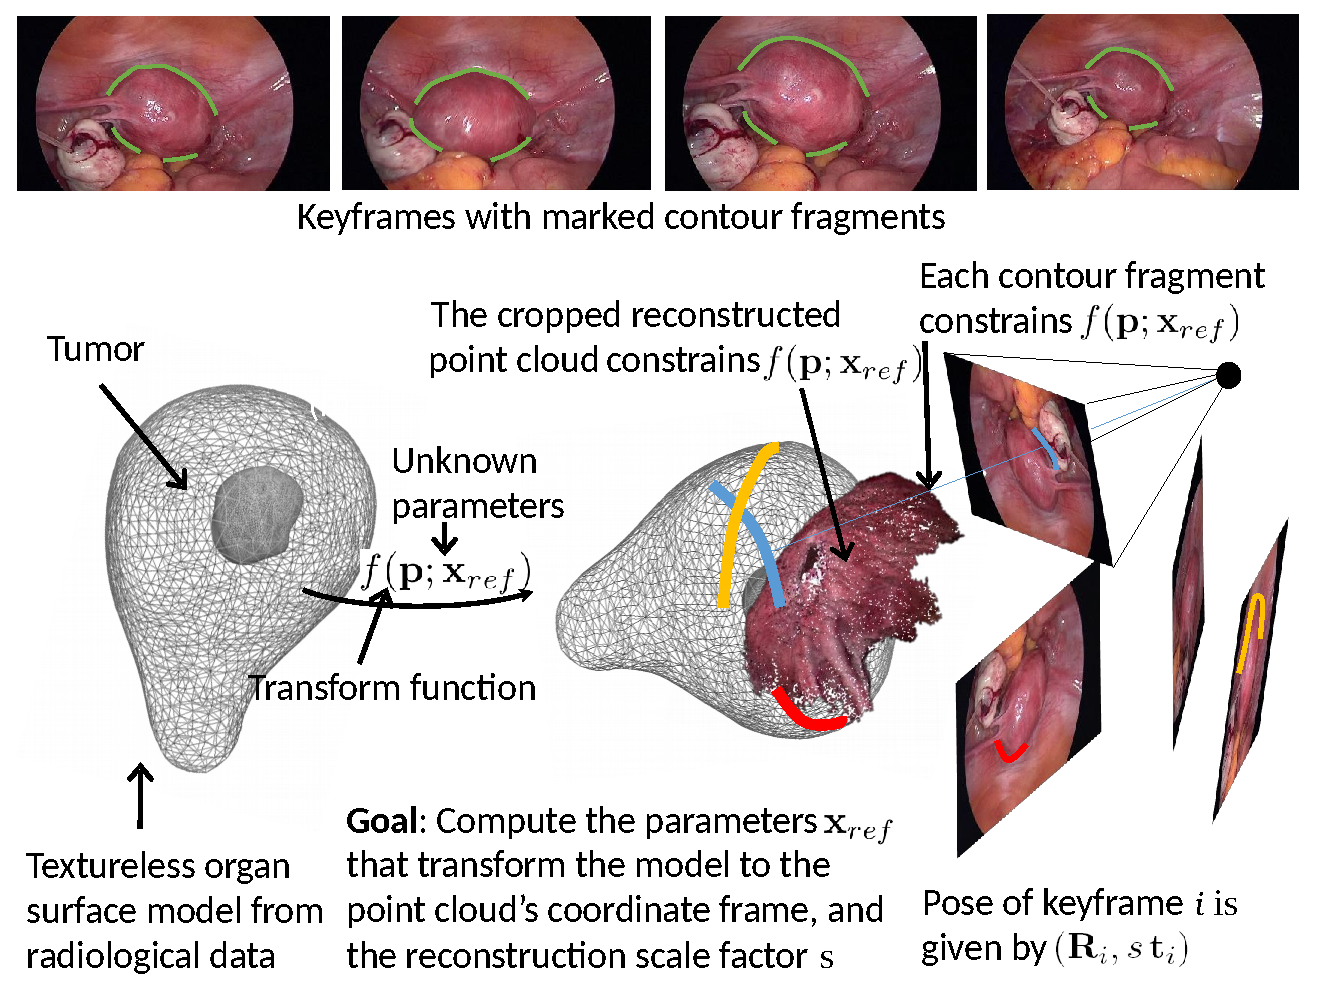
\includegraphics[width=0.9\columnwidth]{./figs/reconstructionDemoNew.pdf}
	\caption{The initial registration problem illustrated on a patient case. Four keyframes from the exploratory video are shown in the first row with their associated silhouette contour fragments.}
	\label{fig:initialRegOverview}
\end{figure}

\subsection{Pre-operative Data Requirements}
\label{sec:inputModels}
The system requires a segmented pre-operative 3D organ model, which comprises the organ's surface mesh, and meshes of internal structures that are to be visualized with AR.
In the case of the uterus, internal structures may be the uterine cavity, tumors and safe-tissue margins. %Here the internal structures are tumors and their \emph{safe tissue margin}.
%A safe tissue margin is a border around the tumor of healthy tissue which should also be removed, whose thickness $w$ depends on the risk factor of the particular tumor.
Our approach does not require a specific organ deformation model to be used, because to date there is no clear consensus on the best one to use for registering organs. %Models currently range from complex heterogeneous mechanical models to simpler homogeneous algebraic models such as As-Rigid-As-Possible \cite{Sorkine:2007:ASM:1281991.1282006}. 

We require two interfaces to the deformation model. 
The first is the \emph{transform function} $f(\vet{p};\vet{x}_t): \Omega\rightarrow \mathbb{R}^3$.
Given the model's parameters $\vet{x}_t$ at time $t$, it transforms a 3D point $\vet{p}$ of the model's 3D domain $\Omega\subset \mathbb{R}^3$ to the laparoscope coordinate frame. 
The second interface is the internal energy function $\Einternal(\vet{x}_{t}):\mathbb{R}^{d}\rightarrow\mathbb{R}^{+}$, with $d$ the dimensionality of $\vet{x}_{t}$. This returns the internal energy for transforming the organ according to  $\vet{x}_t$.
% We require two interfaces to the deformation model. The first is the \emph{transform function} $f(\vet{p};\vet{x}_t): \Omega\rightarrow \mathbb{R}^3$: it is used to transforms a 3D point $\vet{p}$ of the model's 3D domain $\Omega\subset \mathbb{R}^3$ to the target coordinate frame (in our case, the laparoscope coordinates frame). The vector $\vet{x}_t$ denotes the model's parameters at time $t$. %The registration problem is  to determine $\vet{x}_t$ given a laparoscopic image at time $t$. 
% The second is the internal energy function $\Einternal(\vet{x}_{t}):\mathbb{R}^{d}\rightarrow\mathbb{R}^{+}$ which gives the internal energy for transforming the organ with $\vet{x}_t$, where $d$ is the dimensionality of $\vet{x}_{t}$. 
This internal energy is used to regularize the deformation, or in the case of mechanical models, to provide internal strain energy induced by soft-tissue deformation.
We only require that $f$ and $\Einternal$ be continuous and at least first-order differentiable, which is satisfied by virtually all models of interest.
%We describe the specific deformable models used in our experiments in Section \ref{sec:experiments_Simulation}.
 
\subsection{Registration Pipeline Overview}
\label{sec:globalOverview}
Our task is to compute $\vet{x}_t$ for a given live monocular laparoscopic image.
We break down registration into two stages. The first is the \textit{initial registration stage} and the second is the \emph{tracking stage}. 
The initial registration is important for two main reasons. Firstly, the different patient posture between pre-operative and intra-operative steps and the insufflation may induce a significant deformation of the organ. Initial registration estimates such change of shape from the pre-operative to the intra-operative state, or \emph{reference state}. 
Secondly, during the tracking stage, we assume that the organ does not undergo significant deformations so that the tracking stage can be reasonably modeled with rigid motion.  The initial registration allows us to associate texture with the organ's surface, necessary to achieve tracking.
% The purpose of the initial registration stage is two-fold. Firstly, it estimates the change of shape of the organ between its pre-operative state and an intra-operative state, called the \emph{reference state}, caused by physiological movement between pre-operative and intra-operative states, such as patient posture difference and insufflation. Secondly, it associates texture with the organ's surface, which is required in the tracking stage.
% To achieve high robustness we make a simplifying assumption in the tracking stage, which is that the organ does not deform significantly during this stage.
% To simplify the problem, we assume that during the tracking stage the organ does not deform significantly. Therefore, the tracking stage can be modelled with rigid motion, which can be estimated far more quickly and robustly than deformable motion. 

Formally, the two stages of registration break down $f(\vet{p};\vet{x}_t)$ as $f(\vet{p};\vet{x}_{t})=M(f(\vet{p};\xref);\mat{R}_{t},\vet{t}_{t})$. Here \xref denotes the organ's unknown deformation corresponding to the reference state.
The function $M(\cdot;\mat{R}_{t},\vet{t}_{t}):\mathbb{R}^3\rightarrow \mathbb{R}^3$ denotes the unknown update transform at time $t$, parameterized by a rotation $\mat{R}_{t}\in \mathcal{SO}_{3}$ and translation $\vet{t}_{t}\in \mathbb{R}^3$.
%Thus, the initial registration stage estimates $\vet{x}_{ref}$ and the tracking stage estimates $(\mat{R}_{t},\vet{t}_{t})$.

In practice, the rigidity assumption during tracking is reasonable because during the period of live AR guidance the surgeon does not deform the organ in a significant way.
% In practice, rigidity during tracking is a good assumption when the surgeon does not significantly deform the organ during the tracking stage (\ie the period that they wish to use live AR guidance). 
We emphasize that the intended use of AR is to assist spatial comprehension of internal structures and intra-operative resection planning. Typically this is done by guiding the marking of a tumor resection plane on the uterus surface with a coagulation instrument. Such marking is standard practice in uterine surgery. During the actual resection, AR visualization can be deactivated because the assumption of rigid organ motion is no longer valid, and the surgeon can be guided by the coagulation marks.

To provide real-time AR, only the tracking stage needs to be real-time. To minimize workflow interruption, we require the initial registration to be computed in no longer than a few minutes. 
The manual pre-processing takes on average $\sim\SI{2}{\minute}$ while the optimisation takes on average $\sim\SI{1}{\minute}$.
% With our current implementation this takes approximately three minutes on a standard workstation PC (approximately two minutes for manual pre-processing and one minute for optimisation). 
The tracking stage is an optimized implementation in \CC/CUDA and runs at approximately $\SI{25}{fps}$.

%!TEX root=./main.tex

%\section{Phase 1: Semi-automatic Registration of a Preoperative MRI to multiple Intraoperative Reference Images}
%% \subsection{The Initial Registration Stage}
%\label{sec:initialRegistration}
\subsection{Solving the Initial Registration}
\label{sec:registrationOverview}

\subsubsection{Solution Overview}
\fig{fig:initialRegOverview} shows the initial registration problem, which is challenging to solve for two main issues: \textit{(i)} the model to be registered is textureless and \textit{(ii)} the registration is non-rigid.
% We illustrate the problem in \fig{fig:initialRegOverview}. This stage is more challenging to solve than the tracking stage because \textit{(i)} we have no texture information associated with the organ's surface and \textit{(ii)} it is a deformable registration. 
To overcome these problems, our approach includes a dense 3D reconstruction of the organ's surface using an \emph{exploratory video} and SfM/MVS reconstruction, for which mature and open-source methods exist~\cite{Meshroom}. Given this reconstruction, we solve the initial registration with numerical optimization of a system that combines data constraints (organ-to-reconstruction distances and contour fragment distances) with constraints from the model's internal energy.

\subsubsection{Interventional 3D Reconstruction}
\label{sec:sfm}
%To perform the 3D reconstruction, sample images of the organ from different viewpoints and distances are required, known as \emph{keyframes}. We gather these as the surgeon performs an initial exploration of the organ (referred to as the \emph{exploratory phase}), 
During the exploratory video, the uterus is rotated by the surgeon's assistant using the cannula (\fig{fig:cannula}). It moves independently of background structures, so the scene cannot be reconstructed using SLAM, which requires the scene to be globally rigid. 
%Short version
% \SG{We developed a tool to automatically capture sharp keyframes with significant spatial displacement, as this improves the MVS reconstruction quality. We track SIFT features in the live feed using~\cite{Bouguet2001} and, based on the magnitude of their average 2D displacement, the UI hints when a new keyframe can be captured inviting to hold the camera still. On average we capture $N=15$ keyframes.}
%Extended version
\SG{We developed a new tool to capture sharp keyframes with significant mutual spatial displacement.
We extract SIFT keypoints from a frame and track them along the frames of the live feed~\cite{Bouguet2001}.
When the average 2D keypoint displacement exceeds a threshold (default, $\SI{100}{pixels}$) or too many keypoints are lost \wrt the initial frame (default, \SI{35}{\percent}), we consider that the camera has sufficiently moved. We are then ready to acquire a new keyframe and the UI  asks the surgeon to hold the camera still.
We then extract and track new keypoints and the keyframe is acquired when the maximum displacement remains below a threshold (default, $\SI{3}{pixels}$) for the last $M=15$ frames.
Then the process starts again until at least $N=15$ keyframes are acquired.}
% We then extract $N$ keyframes $\{K_1,\dots K_N\}$ (see \fig{fig:cannula}) with a default of $N=10$. We index these with $i\in [1,N]$. This is done by uniformly sampling the video into $N$ intervals. %  with a default $N=12$. 
% We sample the video into $N$ intervals (in practice, $N=10$) and we extract $N$ keyframes $\{K_1,\dots K_N\}$ (see \fig{fig:cannula}), one for each $i\in [1,N]$. 
% In order to select sharp images, which greatly improves the MVS reconstruction quality, each keyframe $K_i$ is select to be the one with the lowest visual motion. In order to assess the quantity of motion between consecutive frame pairs we compute the Sum-of-Absolute Difference (SAD) as measure of similarity.
% We sample the video into $N$ intervals (in practice, $N=10$) and we extract $N$ keyframes $\{K_1,\dots K_N\}$ (see \fig{fig:cannula}). 
% For each interval $i\in [1,N]$ we take the keyframe $K_i$ to be the one with the lowest visual motion, using the Sum-of-Absolute Difference (SAD) as the metric computed between consecutive frame pairs. This is done to improve the quality of the reconstruction because MVS works best with sharper images.
We use a touch-screen interface to manually segment the uterus roughly in the keyframes, so that the background is masked and only the organ is reconstructed. This takes a few seconds per keyframe.
% We then run a state-of-the-art dense SfM\&MVS open source library~\cite{AliceVision}. This provides a dense 3D point cloud $\mathcal{Q}\overset{\mathrm{def}}{=}\{\vet{q}_{1},\dots,\vet{q}_{M}\}$, $\vet{q}_{j}\in\mathbb{R}^{3}$, and the keyframe camera pose matrices $\mat{M}_i \in \mathcal{SE}_4$.
% These hold the laparoscope's rotation matrix $\mat{R}_{i}\in\mathcal{SO}_3$ and translation vector $\vet{t}_{i}\in\mathbb{R}^3$ relative to the point cloud. Recall that an MVS reconstruction is computed up to an unknown global scale factor $s$. We solve for $s$ jointly with registration.
We then run a state-of-the-art SfM/MVS open source library~\cite{AliceVision}. 
As output we obtain a dense 3D point cloud $\mathcal{Q}\overset{\mathrm{def}}{=}\{\vet{q}_{j}\}$, $\vet{q}_{j}\in\mathbb{R}^{3}$, and, for each keyframe, the relevant camera pose matrix $\mat{M}_i \in \mathcal{SE}_4$, holding the rotation matrix $\mat{R}_{i}\in\mathcal{SO}_3$ and translation vector $\vet{t}_{i}\in\mathbb{R}^3$ \wrt the point cloud.
We recall that all MVS reconstructions are  only computed up to an unknown global scale factor $s$. We solve for $s$ jointly with registration in \S\ref{sec:enOpt}.



%Recall that $\mathcal{Q}$ and $\vet{t}_i$ are defined up to the unknown scale factor $s\in\mathbb{R}^+$.
% We chose Photoscan because it has been shown to work well on laparoscopic data~\cite{Collins2013} and can produce far denser reconstructions than purely feature-based methods.

%There may exist some keyframes whose pose is not computable due to, \eg, insufficient visual overlap.
%We currently deal with this by simply removing the keyframe.
%Moreover, the point cloud $\mathcal{Q}$ may contain background and/or foreground structures that partially occlude the organ.
%In this case the human operator can crop them using a fast lasso-based user interface.
%To reduce time we do not require the cropping to be perfect.
%We allow some non-organ points to remain in $\mathcal{Q}$ and we deal with them by making the associated data term robust (see below).
 %There exist a large number of SfM packages one can use such as~\cite{visualSfM3DV,visualSfM3DVWebPage,photoscan}. We currently use Agisoft's Photoscan~\cite{photoscan} because it has been shown to work well on laparoscopic data~\cite{Collins2013} and can produce far denser reconstructions than purely feature-based methods. 
%In some instances SfM may fail, which typically occurs when the keyframe overlap is insufficient.
%This can usually be resolved by extracting more keyframes by doubling the number of intervals and re-running SfM.
%In the rare events in which SfM still fails, \eg, due to very weak texture, we find that image enhancement such as Storz's CLARA can help.
% Alternatively, SLAM could be tried because unlike SfM it exploits temporal continuity.

%Differently than~\cite{Collins2044} which used Photoscan~\cite{photoscan} as MVS tool, we used Meshroom~\cite{Meshroom}, which is an open-source 3D reconstruction software based on the photogrammetric library AliceVision~\cite{AliceVision}. 
%This can be easily integrated in our pipeline and it offers the advantage of easily customizing the settings and the reconstruction parameters to produce high quality 3D models.

\begin{figure}[t]
  \centering
  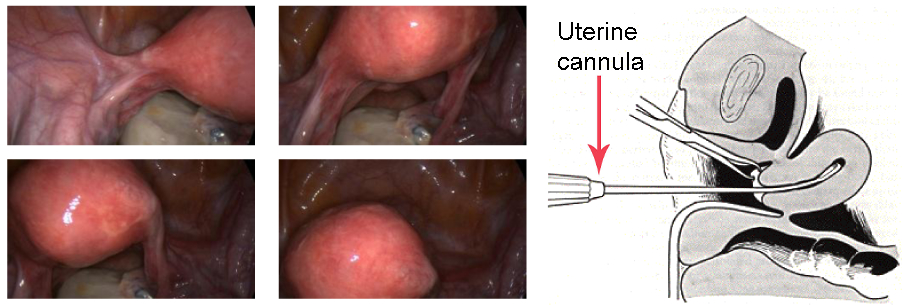
\includegraphics[width=0.79\columnwidth]{./figs/exploratory.pdf}
  \caption{Example keyframes from an exploratory video of a uterus undergoing cannula motion.}
	\label{fig:cannula}
\end{figure}


%In our experiments typically no more than $10$ images are required to obtain a good quality reconstruction.

%\begin{figure}[h]
%	\centering
%	\includegraphics[width=1.0\textwidth]{./figs/segmentationAndModel.pdf}
%	\caption{CAPTION}
%	\label{fig:deformableModel}
%\end{figure}

%\begin{figure}[h]
%	\centering
%	\includegraphics[width=1.0\textwidth]{./figs/optimisationTable.pdf}
%	\caption{CAPTION}
%	\label{fig:sfmExample}
%\end{figure}

%We summarise the initial registration process as follows. This is similar to~\cite{Collins2044} but with some important improvements that we list at the end of the paragraph. First a rough initialisation is made using a rigid transform and a small amount of manual assistance. 

\subsubsection{Silhouette Contours}
An occluding contour is a boundary in a 2D image between an object surface and another surface that is further away, that it partially occludes. This includes  \emph{self-occluding contours}, which are formed where the object self-occludes, and \emph{silhouette contours}, which are formed by the object and a background structure. Most organs are approximately convex, so self-occluding contours are rare events. \SG{By} contrast, silhouette contours are common, and we propose to use these to constrain the organ's shape during registration. We require the silhouette contours to be provided in a keyframe image (\fig{fig:initialRegOverview}). This is very difficult to automate because not all of the organ's boundaries in an image correspond to silhouette contours. Indeed, they are either silhouette contours, or contours formed by the silhouette of another structure occluding the organ. We illustrate this in \fig{fig:initialRegOverview} (top row) where abdominal fat occludes the posterior region of the uterus. The boundary between fat and the uterus conveys no information about the shape of the uterus.  
%we must both recover the organ's boundaries in an image, and infer which of those are silhouette contours compared with contours formed by another structure occluding the organ. 

Consequently, extracting an organ's silhouette contours cannot be solved directly by organ segmentation, because this does not distinguish the above contour types. Furthermore, organ segmentation is itself a hard problem with laparoscopic images. We therefore propose to extract silhouette contours with a fast semi-automatic process and a touch-screen interface. \SG{The keyframes are displayed} and the operator traces the organ's silhouette contours with a finger stroke. We apply the method of~\cite{Mortensen95intelligentscissors} to snap the finger stroke to the nearest image contour, based on active contours attracted to the dominant image edge adjacent. This is very fast and a keyframe is processed in a matter of seconds. %Occasionally, snapping may fail mainly in cases where the contour fragment is very low contrast. In these cases the operator sets the contour to inactive, meaning that it is not used during registration. 



%We define a \emph{contour fragment} as a connected path in a keyframe image that corresponds with the organ's occluding contour. Recall that 

%%%%%%%%%%%%
%We formulate the problem as a non-linear energy-minimisation problem, with energies coming from prior and data terms.
%The prior term encodes the model's internal energy, which is used to regularise the problem.
%The data terms are illustrated in \fig{fig:initialRegOverview}.
%The first involves the point cloud reconstruction, and encourages the organ's surface mesh to fit to the point cloud.
%Importantly, this is a \emph{robust} data term, which accounts for the fact that the reconstruction may contain outliers or some residual background and/or occluding structures.
%The second data term complements the first and uses contour cues.
%Specifically, it is a silhouette contour term which makes the organ model's silhouette align to its associated contours in the keyframe images.
%This is complementary to the point cloud data term for two reasons.
%Firstly, we never usually reconstruct points reliably at these regions due to occlusions.
%Secondly, it anchors the organ's silhouette to the contour fragments, which is a strong constraint.
%We implement this data term with some manual assistance: a human operator marks in a keyframe where they can confidently see the organ's silhouette contours (\fig{fig:initialRegOverview}, first row).
%We call these \emph{contour fragments}.
%The operator does not need to mark contour fragments in all keyframes (it can be done with only one).
%If more keyframes are marked then we have more constraints marking contour fragments.
%Differently than our previous work~\cite{Collins2044}, the user can now mark these contours by means of a touch-screen interface using rough finger strokes.
%These strokes then guide an automatic refinement method based on intelligent scissors~\cite{Mortensen95intelligentscissors}.
%This reduces manual effort and speed up the process, which now typically takes, overall, less than $\SI{10}{\second}$ for a single keyframe.
%In general, $4$ to $6$ keyframes are enough.
%They also do not need to be contiguous. \todo{necessary to say?}
%Optionally, an anatomical landmark data term can also be included, which is used to align distinct landmarks that can be found on the organ's surface in the pre-operative and laparoscopic images.
%In the case of the uterus these can be the Fallopian tube/uterus junctions, which were manually located.
%Landmarks help guide the registration if the initialisation is poor or there is very strong deformation.
%In the presented experiments we do not use them in the optimisation process, so they are omitted from the energy function. 
%%%%%%%%%%%%%%%%%%%%%%%%


% The main improvements over~\cite{Collins2044} are summarised as follows:

%\paragraph{Overview.}
%We solve the initial registration in a similar way as described in~\cite{Collins2044} but with several key improvements. This is based on an energy-minimisation process where the energy encodes optical registration constraints from the keyframes and deformation priors from the organ's physical material. The energy is robust to handle common errors when pre-processing the keyframe images (\eg imperfect segmentation), and is minimised with iterative numerical optimisation. This requires an initial solution which can be computed depending on the context. We give details for how the initial solution is computed for the user study at the end of this section. An important assumption for solving the initial registration is that the organ does not deform during the exploratory phase. This allows us to reconstruct the interventional environment \emph{in 3D} with rigid Structure-from-Motion (SfM). With live organs slight deformation may be unavoidable, however if the deformations are small compared to the camera's motion then we can usually reconstruct the laparoscopic environment with a state-of-the-art dense SfM algorithm. The benefit of reconstructing the environment is twofold. Firstly, it allows us to calibrate the keyframe images, and this enables us to use \emph{all} keyframe images to constrain the initial registration problem. The second benefit is that the reconstruction gives information for the interventional 3D shape of the organ, which can be used to constrain the registration problem.

%\paragraph{Summary of improvements to~\cite{Collins2044} for solving the initial registration.} The main improvements are as follows:

% \begin{enumerate}[-,topsep=1pt]
% 	\item In~\cite{Collins2044} the deformable model used was a 3D affine model. 
%   This was shown to be sufficient for simple deformations of the human uterus but is not sufficient in general.
% We extend the approach to work with general biomechanical models.
% This requires changing the core energy function to include the model's internal energy (without this the problem is highly under-constrained), and to correct the interventional reconstruction's scale factor $s$.
% Note that in~\cite{Collins2044}, $s$ could be absorbed into the affine model's coefficients.
% This is generally not possible with biomechanical models because a change of scale affects the internal energy.
	
% 	\item In~\cite{Collins2044} the organ's surface was assumed to have disc topology.
% We  generalise this to arbitrary fixed topologies.
% 	\item We have sped up the process of marking contour fragments considerably with a touch-screen interface, where the operator marks them with rough finger strokes.
% These strokes then guide an automatic refinement method based on intelligent scissors~\cite{Mortensen95intelligentscissors}.
% This reduces manual effort, typically taking less than $\SI{10}{\second}$ for a single keyframe.
% \end{enumerate}  






 %Example keyframes and a dense SfM reconstruction for one of the user study kidneys is shown in Figure %\begin{figure}[h]
%	\centering
%	\includegraphics[width=1.0\textwidth]{./figs/sfm2.pdf}
%	\caption{CAPTION}
%	\label{fig:exampleKeyframesAndSfM}
%\end{figure}


%\paragraph{Contour fragments.} A human operator then traces contour fragments in one or more keyframes (we use a default of 4 uniformly sampled in time) using the touch-screen interface and intelligent scissoring, as described in point 3 above. This is a very fast process, however occasionally errors can happen when the fragment does not correctly snap to the right image position. This mostly occurs if the edge contrast is low. This could be dealt with by having the operator manually re-trace it without intelligent scissoring, but it would cost time. Instead we say that some errors in the contour fragments are unavoidable, and we deal with them by making the associated data term \emph{robust} to such errors, as described below. 

\subsection{Initialization}
\label{sec:Initialization}
Initially, \xref is initialized with a rigid transform $\mat{M}_a\in \mathcal{SE}_4$.
If the laparoscope is in a canonical position \wrt the organ, $\mat{M}_a$ can be considered known \emph{a priori}.
Otherwise, we devised an interactive and relatively simple procedure to provide a rough estimate of $\mat{M}_a$.
The method is based on solving PnP~\cite{Lepetit2009Epnp} between 3D points on the organ's surface model and their corresponding 2D points on one of the keyframes, selected interactively.
The operator can first freely rotate the 3D model to present it from a similar viewpoint as the keyframe.
\SG{Then they select at least $5$ 3D points on the 3D model and their corresponding points on the image.
We found that a good strategy is to select the $4$ equidistant points on the image along (but not on) the occluding contour and one roughly in the middle.
The corresponding points on the 3D model can be guessed following the same pattern.
Associating points from an untextured 3D model to its image is not in general a trivial task but we found that surgeons can easily perform the operation thanks to their detailed understanding of the anatomy.
The correspondences are not required to be accurate, as this only serves as rough initialization of the camera pose.}
%The estimated camera pose is used to initialize  $\mat{M}_a$.

% We initialize \xref with a rigid transform, denoted by $\mat{M}\in \mathcal{SE}_4$.
% In some cases $\mat{M}$ can be considered known \emph{a priori}, \eg if the laparoscope is assumed to be in a canonical position with respect to the organ.
% When this cannot be assumed, we compute it with a small amount of manual interaction as follows.
% A small number of point correspondences (at least four) are selected on the organ's surface model and one of the keyframe images.
% Without loss of generality, let this be the first keyframe $K_1$.
% We then compute a rigid transform  $\mat{M}_a$ from model coordinates to laparoscope coordinates, by fitting the correspondences using a PnP method~\cite{Lepetit2009Epnp}.
% The point correspondences are computed using an interactive user interface, where the model can be freely rotated to present it from a similar viewpoint as the keyframe's viewpoint. This significantly eases the operator's task. 

To provide an initialization of the reconstruction scale factor $s$, we apply $\mat{M}_a$ to the model.
We then use OpenGL to render a synthetic image of it using the calibrated intrinsic parameters of the laparoscope. 
OpenGL's $z$-buffer provides a depth map $d(x,y)$ from which we can compute $s$ by comparing depths in $d$ to depths in $\mathcal{Q}$.
% We initialize the reconstruction scale factor $s$ as follows. First we transform the model by $\mat{M}_a$ and render it using the OpenGL rendering engine, using the same intrinsic parameters as the laparoscope, thus obtaining a depth map $d(x,y)$ from OpenGL's $z$-buffer. We then compute $s$ by comparing depths in $d$ to the depths of $\mathcal{Q}$. 
Specifically, for a 3D point $\vet{q}_j$, an estimate of $s$ is  $s_j=d(x_j,y_j)/\tilde{d}_j$, where $\tilde{d}_j$ is the depth of $\vet{q}_j$, and $(x_j,y_j)$ its corresponding 2D point.
The robust estimate is given by the median over all points, $s=\mathrm{median} \{s_j\}$. 

% Specifically, let $\tilde{d}_j$ be the depth of $\vet{q}_j$ in keyframe $K_1$, and $(x_j,y_j)$ be its 2D position in the keyframe's image. We can then estimate $s$ by $s\approx d(x_j,y_j)/\tilde{d}_j$. To compute $s$ robustly, we use the median estimate using all points. Finally, the transform $\mat{M}$ is given by the composition $\mat{M} = \mat{M}_s\,\mat{M}^{-1}_i\,\mat{M}^{-1}_s\,\mat{M}_a$, where $\mat{M}_s$ is an isotropic scaling by $s$. 

\subsection{Energy-based Optimization}
\label{sec:enOpt}
We describe the registration energy function and optimization process. To improve clarity we assume all image points in normalized camera coordinates, which is obtained from the intrinsic calibration, and thus define camera projection as
$\pi(\left[x,y,z\right]^{\top})\overset{\mathrm{def}}{=}\left[x,y\right]^{\top}/z$. 
Besides the model's internal energy $\Einternal(\vet{x})$, the energy function $E(\vet{x},s)\in\mathbb{R}^+$ consists of two other terms.
We introduce a point cloud data term \Epoint to help the organ's surface fit the reconstructed point cloud.
To constrain the organ's silhouette contours to fit the silhouette contour fragments we also include a contour data term \Econtour. 
Thus, the energy $E(\vet{x},s)$ is defined as:
\begin{equation}
\label{eq:totalCost}
\begin{split}
E(\vet{x},s)=\Epoint(\vet{x},s;\mathcal{Q}) & + \lambdaContour\Econtour(\vet{x},s)
% \\;\mathcal{C}_{1},\dots ,\mathcal{C}_{N}
% & 
+\lambdaInternal\Einternal(\vet{x}),
\end{split}
\end{equation}
\noindent where $\lambdaContour$ and $\lambdaInternal$ are scalar weights (\SG{with defaults} $\lambdaContour=100$ and $\lambdaInternal=50$).

% The energy function $E(\vet{x},s)\in\mathbb{R}^+$ consists of the point cloud data term \Epoint, which encourages the organ's surface to fit to the reconstructed point cloud $\mathcal{Q}$, the contour data term \Econtour, which encourages the organ's silhouette contours to fit to the silhouette contour fragments, and the model's internal energy $\Einternal(\vet{x})$:
% \begin{equation}
% \label{eq:totalCost}
% \begin{split}
% E(\vet{x},s)=\Epoint(\vet{x},s;\mathcal{Q}) & + \lambdaContour\Econtour(\vet{x},s;\mathcal{C}_{1},\dots ,\mathcal{C}_{N})\\
% & +\lambdaInternal\Einternal(\vet{x}),
% \end{split}
% \end{equation}
% \noindent where $\lambdaContour$ and $\lambdaInternal$ are scalar weights (typically, $\lambdaContour=100$ and $\lambdaInternal=50$).
% The set $\mathcal{C}_i$ denotes all pixels on the contour fragments in keyframe $i$. 

For the point cloud data term \Epoint we use an ICP-based energy term: it uses a set of \emph{virtual point correspondences} $\mathcal{P}=\{\vet{p}_j\}$ with $|\mathcal{Q}|=|\mathcal{P}|$, where $\vet{p}_j\in\partial \Omega$ is the unknown position of point $\vet{q}_{j}$ on the organ's surface mesh $\Omega$.
For a given $(\vet{x},s)$, \Epoint is computed by first transforming $\Omega$ according to $\ensuremath{f(\cdot;\vet{x})}$ and applying the estimated scale factor $s$ to the point cloud, so that $\hat{\vet{q}}_{j}\gets s\,\vet{q}_{j}$.
Then, $\vet{p}_j$ is set to the closest point to $\hat{\vet{q}}_{j}$ on the surface's mesh.
Similarly to the point-to-plane distance function of ICP with rigid objects, \Epoint uses a robust point-to-plane distance function that allows the model to slide over the point cloud without resistance:
\begin{equation}
\Epoint(\vet{x},s;\mathcal{Q})=\frac{1}{M}\sum_{j=1}^{M}\rho\left(\dplane\left(v_{j}(\vet{x}),\hat{\vet{q}}_{j}\right)\right),
\end{equation}
where $v_{j}(\vet{x})\in\mathbb{R}^4$ gives the organ surface's tangent plane at $f(\vet{p}_{j})$.
The function $\dplane(\vet{v},\vet{q})$ gives the signed distance between a plane $\vet{v}$ and a 3D point $\vet{q}$.
The function $\rho:\mathbb{R}\rightarrow\mathbb{R}^{+}$ is an \emph{M-estimator}. % and it is designed to robustly align the reconstructed point $\hat{\vet{q}}_{j}$ with the organ's surface. 
The MVS reconstruction may contain points off the organ or poorly reconstructed; these are discarded by the M-estimator.
We experimented with different types of estimators and found that a pseudo-L1 $\rho({x})\overset{\mathrm{def}}{=}\sqrt{{x}^{2}+\epsilon}$ offers good results (\SG{with default} $\epsilon = 10^{-4}$).

% We construct \Epoint using an ICP-based energy term.
% This works using a set of \emph{virtual point correspondences} $\mathcal{P}=\{\vet{p}_1,\dots \vet{p}_M\}$ with $\vet{p}_j\in\partial \Omega$ denoting the unknown position of point $j$ on the organ's surface mesh. 
% For a given $(\vet{x},s)$ we compute \Epoint as follows. First we transform the organ's surface mesh according to $\ensuremath{f(\cdot;\vet{x})}$ and rescale the point cloud with $\hat{\vet{q}}_{j}\gets s\,\vet{q}_{j}$.
% We then set $\vet{p}_j$ as the closest point to $\hat{\vet{q}}_{j}$ on the surface's mesh.
% We define \Epoint using a robust point-to-plane distance function, which is inspired by point-to-plane ICP with rigid objects.
% This allows the model to slide over the point cloud without resistance, and is defined as follows:
% \begin{equation}
% \Epoint(\vet{x},s;\mathcal{Q})=\frac{1}{M}\sum_{j=1}^{M}\rho\left(\dplane\left(v_{j}(\vet{x}),\hat{\vet{q}}_{j}\right)\right).
% \end{equation}
% \noindent The function $v_{j}(\vet{x})\in\mathbb{R}^4$ gives the organ surface's tangent plane at $f(\vet{p}_{j})$.
% The function $\dplane(\vet{v},\vet{q})$ gives the signed distance between a plane $\vet{v}$ and a 3D point $\vet{q}$.
% The function $\rho:\mathbb{R}\rightarrow\mathbb{R}^{+}$ is an \emph{M-estimator} and is crucial to achieve robust registration.
% Its purpose is to align the reconstructed point $\hat{\vet{q}}_{j}$ with the organ's surface, but to do so robustly to account for non-organ points being in $\mathcal{Q}$ or poorly reconstructed points.
% The model should not align these points, and the M-estimator facilitates this by reducing their influence on the energy.
% We have tested various types and good results are obtained with pseudo-L1 $\rho({x})\overset{\mathrm{def}}{=}\sqrt{{x}^{2}+\epsilon}$ with $\epsilon = 10^{-4}$.

Similarly, \Econtour uses virtual point correspondences on the organ surface mesh's occluding contours.
More explicitly, for a given estimate $(\vet{x},s)$ and a given keyframe $i$, we generate a set of virtual correspondences $\mathcal{R}_i=\{\vet{r}_1,\dots ,\vet{r}_{C(i)}\}$
containing, for each contour pixel $\vet{c}_k$, the unknown position $\vet{r}_k\in\partial \Omega$  of its corresponding 3D point on the model's surface.
To compute the correspondence we first apply $\ensuremath{f(\cdot;\vet{x})}$ to the organ's surface mesh, and we bring the model in the reference frame of the camera $i$ using $(\mat{R}_{i}, s\,\vet{t}_{i})$.
Then
% , using the same intrinsic parameters as the laparoscope, 
we render the surface mesh as described in \sect{sec:Initialization} and store all the pixels on the silhouette boundary in a set $\mathcal{B}$. 
Let $\mathcal{C}_i$  the set of all pixels belonging to the contour fragments in keyframe $i$.
We compute for each contour pixel $\vet{c}_k\in \mathcal{C}_j$ its closest point $\vet{b}_k\in \mathcal{B}$.
Finally, we set $\vet{r}_k$ as the 3D position of $\vet{b}_k$, computed using the render's depth buffer.
From all the correspondences $\mathcal{R}_i$, \Econtour is computed as:
\begin{equation}
\label{eq:contour}
\begin{split}
% ;\mathcal{C}_{1},\dots,\mathcal{C}_{N}
 & \Econtour(\vet{x},s) = \frac{1}{C}\sum_{i=1}^{N}\sum_{\substack{\vet{c}_{k}\in\mathcal{C}_{i}\\\vet{r}_{k}\in\mathcal{R}_{i}}}\rho\left(\|\pi\left(f(\vet{r}_{k})\right)-\vet{c}_{k}\|\right),
\end{split}
\end{equation}
\noindent where $C$ is the total number of contour fragment pixels.
Similarly to \Epoint, we use the M-estimator $\rho$ for robustness.

% We construct \Econtour similarly with virtual point correspondences.
% Specifically, for a given pair $(\vet{x},s)$ and a given keyframe $i$ we construct a set of virtual correspondences $\mathcal{R}_i=\{\vet{r}_1,\dots ,\vet{r}_{C(i)}\}$ where $\vet{r}_k\in\partial \Omega$ denotes the unknown position of the $k^{th}$ contour fragment pixel $\vet{c}_k$ on the model's surface.
% The virtual correspondences are points on the organ surface mesh's occluding contours, and are computed as follows.
% First we transform the organ's surface mesh according to $\ensuremath{f(\cdot;\vet{x})}$, then transform it to laparoscope coordinates using $(\mat{R}_{i}, s\,\vet{t}_{i})$.
% We render the surface mesh, using the same intrinsic parameters as the laparoscope.
% We then take the render's silhouette and store all the pixels on the render's boundary in a set $\mathcal{B}$.
% For each contour fragment pixel $\vet{c}_k\in \mathcal{C}_j$ we compute its closest point $\vet{b}_k\in \mathcal{B}$  and form a correspondence with it.
% We then compute the 3D position of $\vet{b}_k$ using the render's depth buffer, and assign this position to $\vet{r}_k$.
% We then evaluate \Econtour as the alignment error from all correspondences:
% \begin{equation}
% \label{eq:contour}
% \begin{split}
%  & \Econtour(\vet{x},s;\mathcal{C}_{1},\dots,\mathcal{C}_{N}) = \\ 
%  &  \frac{1}{C}\sum_{i=1}^{N}\sum_{\substack{\vet{c}_{k}\in\mathcal{C}_{i}\\\vet{r}_{k}\in\mathcal{R}_{i}}}\rho\left(\|\pi\left(f(\vet{r}_{k})\right)-\vet{c}_{k}\|_{2}\right),
% \end{split}
% \end{equation}
% \noindent where $C$ is the total number of contour fragment pixels.
% Here the M-estimator $\rho$ is also used to handle the fact that some contour fragments may be erroneous, which can occurs if the contour fragment incorrectly snaps at low-contrast edges. 

% and we give details for each test case in the experimental section. The weights $\lambdaContour$ and $\lambdaInternal$ are fixed in all experiments at $\lambdaContour=100$ and $\lambdaInternal=50$. 

\subsection{Optimisation}
In order to improve convergence, we use a stiff-to-flexible strategy to optimize $E$. We start with a stiff model, we optimize $E$, and then we reduce the stiffness to account for more deformation.
We usually use $6$ stiffness levels, in which the value of $\lambdaInternal$ is halved \wrt the previous level, \ie $\lambdaInternal(l)=\lambdaInternal(l-1)/2$.
At each level we alternate between computing the virtual correspondence sets ($\mathcal{R}_i$ and $\mathcal{P}$) and optimising $E$, via Gauss-Newton iterations with backtracking line search.
This alternating process proceeds until either convergence or a maximum of $20$ iterations is reached.
% We optimize $E$ using a stiff-to-flexible strategy. This is to improve convergence by starting with a stiff model, optimising $E$, then reducing the stiffness to account for more and more deformation. We use a default of $l=6$ stiffness levels with $\lambdaInternal(l)=2\,\lambdaInternal(l-1)$. For each level we alternate between computing the virtual correspondence sets ($\mathcal{R}_i$ and $\mathcal{P}$) and optimising $E$, via a Gauss-Newton iteration with backtracking line search. This continues until either convergence is reached or $20$ iterations have passed. %At the final stiffness level we optimize until convergence. 
%Convergence however is not guaranteed because of the point-to-plane distance function in \Epoint. Specifically, the energy may increase after $\mathcal{P}$ is re-computed. We handle this by using the point-to-point distance at the final level, because this ensures $E$ will decrease at each iteration, and optimize until convergence.


%!TEX root=./main.tex

\subsection{Real-time Tracking-by-Detection}
\label{sec:updateRegistration}
\subsubsection{Overview}
Once the initial registration is computed,  real-time tracking starts from the live feed of the laparoscope. 
Our approach updates the initial registration at each frame and is robust to common challenges including occlusions (\eg, surgical tools), partial views and viewpoint changes.
% Having solved the initial registration we initiate the tracking stage, which updates the initial registration in real-time using live laparoscopic images. %First we extract features in the keyframe images, then matching them to each new image in a RANSAC framework. 
% This approach is robust to common challenges including occlusions from \eg, surgical tools, partial views and viewpoint changes.

%Unlike SLAM-based tracking methods it does not use frame-to-frame tracking. Instead it performs \emph{tracking-by-detection}. This allows it to keep the registration over long durations and can trivially recover when the organ is not visible for certain periods, such as when the surgeon removes and then reinserts the laparoscope or cleans the lens.
%In cases when the organ is assumed to be fixed relative to background structures, we can track using features from both the organ and background structures.
%This improves stability if the organ's texture is weak, and we do this in the ex-vivo user study. 

\subsubsection{Keypoint Mapping}
\label{sec:preparing}
For each keyframe, we render the 3D model and store the depth map of all the pixels lying within the model's silhouette. %We use $(x,y,z)=rim(i,j)$. to be the 3D position in camera coordinates at pixel location $(i,j)$. If $x=y=z=\mathrm{nan}$ then pixel $(i,j)$ dose not lie within the silhouette of the model, otherwise it dose. We denote $\mat{M}_{i}\in SE_{4}$ to be the rigid transform mapping the model to the $i^{th}$ reference image's frame. We can compute the 3D position of an image point lying with the model's silhouette by $\mat{M}_{i}^{-1}[x,y,z,1]^{\top}$. 
%The RIM is convenient because for each texturemap image we can extract 2D image features \textit{anywhere} within the model's silhouette, 
From this, the 3D position \vet{u} of any 2D image keypoint located within the model's silhouette can be determined.
%Note that without computing a dense 3D model this is not possible in general.
For each keyframe, we then extract a set of image keypoint and to each one of them we associate its corresponding depth. 
\SG{We concatenate the keypoint from all images into a single list $\mathcal{F}=\{(\vet{u}_{m},i_{m},\vet{d}_{m})\}$, where $\vet{u}_{m} \in \mathbb{R}^3$
% denotes the $m^{th}$ feature's 3D position in the model coordinate frame, $I_{m}$ denotes the index of the keyframe from which it was detected and $\vet{d}_{m}$ denotes its descriptor.
is the 3D point associated to feature detected in the keyframe of index $i_{m}$, with $\vet{d}_{m}$ its associated descriptor.}

The approach can be used with any keypoint detector, such as SIFT~\cite{Lowe:2004:DIF:993451.996342}, ORB~\cite{orbslam_laparo} or SURF~\cite{SURF}.
We find that SIFT has better performances in image matching~\cite{Tuytelaars2007}.
We used the recent open-source GPU implementation PopSift~\cite{Griwodz2018Popsift} to achieve real-time computation: for a typical HD $1920\times1080$ image of the uterus, up to $3000$ keypoints can be found in about $\SI{11}{\milli\second}$ with a standard GPU.
%We use the green channel to compute features, rather than the standard approach of using average intensity.
%The reason is that the green light penetrates human tissue superficially and do not exhibit as much sub-surface scattering as with red light.
%The difference is very prominent with the uterus~\cite{DBLP:conf/ipcai/CollinsB12}.
To significantly reduce the problem of wrongly tracking specularities, we detect saturated pixels with an intensity threshold of $250$ and any keypoint within $\SI{5}{pixels}$ to a saturated pixel is discarded.  

\subsubsection{Pose Estimation Overview}
\label{sec:registration}
For each new image we extract a set of keypoints $\mathcal{G}=\{(\vet{y}_{i},\tilde{\vet{d}}_{i})\}$, where $\vet{y}_{i}$ is the 2D image point and $\tilde{\vet{d}}_{i}$ its descriptor. Our registration scheme has three main steps. First, a set of candidate matches between $\mathcal{F}$ and $\mathcal{G}$ is computed and then a pose hypothesis that best explains these matches is searched. Finally the best pose hypothesis is refined with the Levenberg-Marquardt (LM) algorithm by minimizing the reprojection errors.

\subsubsection{Computing Candidate Matches}
Good candidate matches of the sets $\mathcal{F}$ and $\mathcal{G}$ are those pairs with \textit{(i)} strong descriptor agreement (\ie low descriptor distance) and \textit{(ii)} a low likelihood of being false.
We achieve the latter condition by applying Lowe's Ratio Test (LRT)~\cite{Lowe:2004:DIF:993451.996342}.
%For each member of $\mathcal{F}$ we compute the member in $\mathcal{G}$ with the nearest descriptor.
%If this descriptor distance is greater than $\tau$ times the distance to the second nearest descriptor in $\mathcal{G}$, it is deemed a candidate match.
%The LRT is a very standard condition in feature-based pose estimation.
A novelty of using \emph{multiple} keyframes is that we can also exploit match \emph{coherence}. 
Specifically, consider a feature in the image that matches a feature in the $i^{th}$ keyframe. 
It is likely to be correct if there exists other features that also match with features in the $i^{th}$ keyframe.
%Enforcing coherence can reduce false matches because it prevents matches occurring from wildly different keyframe.
We adopt a ``winner-takes-all'' strategy to enforce coherence and reduce false matches.
\SG{Let $i^*$ be the index of the keyframe with the largest amount of candidate matches.
Since SIFT is invariant to scale changes and image rotation, the keyframe $i^*$ can be considered as the visually ``closest'' to the input image.}
% We enforce coherence with a winner-takes-all strategy. We first find the index $I^*$ of the keyframe with the largest amount of candidate matches. This indicates the keyframe image which is ``closest'' to the input image \wrt the viewpoint. Because SIFT is invariant to scale changes and image rotation, %close means a keyframe image which views the uterus from a similar viewpoint, up to a change in depth and a rotation of the laparoscope about its optical axis.
\SG{we then recompute the candidate matches, but using \emph{only} features from the keyframe $i^*$.}
Computational efficiency can be easily achieved as $\mathcal{F}$ is completely pre-computed and the distances to evaluate the descriptor likelihood are quite fast to compute on the GPU (\eg, $\sim\SI{3}{ms}$ to match $2000$ features from an HD image against $5600$ features from $16$ keyframes).
% Performing these processes is very quick because $\mathcal{F}$ is completely pre-computed, and evaluating descriptor distances can be distributed trivially on the GPU (\eg, $\sim\SI{3}{ms}$ to match $2000$ features from an HD image against $5600$ features from $16$ keyframes).

\subsubsection{Computing 3D Pose}
% Given the set of candidate matches, we perform RANSAC~\cite{Fischler:1981:RSC:358669.358692} to find the most compatible rigid 3D pose, with OpenCV's implementation with default parameters. 
From the set of candidate matches, we find the best pose hypothesis that explains these  matches using   RANSAC~\cite{Fischler:1981:RSC:358669.358692} from OpenCV's default implementation.
In some images tracking may be impossible or unreliable, if the organ is not visible or very partially. A good indicator for deciding if pose can be estimated reliably is the number $n_c$ of inlier matches found by RANSAC. If this is below a threshold (default $8$ points), we reject the pose and consider the organ to be untrackable in that image. Finally, to reduce jitter, we feed the pose estimates into an Extended Kalman Filter (EKF). 

\subsubsection{Adding New Keyframes}
The operator can manually add new keyframes to $\mathcal{F}$ on the fly during the live tracking.
This mitigates any remaining jitter and stabilizes tracking if the organ is viewed from a viewpoint that is very dissimilar to the keyframes.
\SG{Adding keyframes also copes with changes occuring between the reference and current intra-operative states in organ appearance (bleeding spots, change of color because of the clamping) and 3D orientation (due to mobilization).}
%In the supplementary material we present a video showing the benefits and the impact of adding a new keyframe to the tracking.
We add the keypoints of the current image and their associated 3D points to $\mathcal{F}$.
We do not automate the process of adding new keyframes because without care it can lead to drift.
Specifically, errors in the estimate pose then lead to incorrectly aligned keypoints in $\mathcal{F}$ and degradation in tracking accuracy.
\SG{The operator can add the current frame as a new keyframe by pressing a bottom on the interface. A still image of the current frame with AR is then shown to the operator for validation.}

%This involves sampling many match subsets of size $4$, and for each sample creating a pose hypothesis using PnP~\cite{Lepetit2009Epnp}.
%Each hypothesis is tested for support by measuring how many of the other matches are predicted well by the hypothesis.
%Sampling and hypotheses testing is highly parallelisable, and we rely on the OpenCV's implementation.
%There are three free parameters which govern performance.
%The first is the number of hypotheses $n_k$ to sample and it represent a upper bound on the number of iterations of the RANSAC process.
%The second is the threshold $\tau_r$ (in pixels) on the reprojection error of the 3D point, below which a match is considered to support a hypothesis.
%The third is the minimum number of matches $n_c$ that must support a hypothesis.
%A larger $n_c$ means we need more matches to be confident that pose has been estimated correctly.
%We have found good default values to be $n_k=500$, $\tau_r= 12$ pixels and $n_c=15$.
%Finally, in order to compensate for the trajectory jittering we used an Extended Kalman Filter (EKF) to smooth the trajectory of the camera.




%If a pose cannot be found no pose has been found with more than $n_c$ supported matches, then we say the uterus' pose cannot be estimated for that image. 

%\subsubsection{Pose optimization and temporal smoothing}
%If enough matches support the computed pose, we then refine the pose with an efficient Gauss-Newton Optimization~\cite{Lepetit2009Epnp}.
%We use only the matches that supports the found pose and we optimize the pose using the OpenCV implementation. 
%Finally, in order to compensate for the trajectory jittering we used an Extended Kalman Filter (EKF) to smooth the trajectory of the camera.


%%%%%PROPOSE TO REMOVE THIS
%\subsubsection{Adding new keyframes}
%%In order to further stabilize and improve the pose computation, we add the possibility for an operator to add new keyframes to $\mathcal{F}$ on the fly during the live tracking. This helps to mitigate any remaining jittering and stabilizes tracking if the organ is viewed from a viewpoint that is very dissimilar to the ones present in the keyframe set.
%%%to complete the coverage of the organ from other viewpoints.
%%%When a j the user decide to add a new keyframe we use a similar procedure as described in \sect{sec:preparing}.
%%We perform this by adding the current image and its estimated pose to the keyframe set, and we add the features of the current image to $\mathcal{F}$. We currently refrain from automating the process of adding new keyframes because without care it can lead to drift. Specifically, errors in the estimate pose then leads to incorrectly aligned features in $\mathcal{F}$, leading to a degradation in tracking accuracy in later frames.

%We render the 3D model in the current camera pose to obtain a depth map of all the pixels lying within the model's silhouette.
%For each extracted feature of the current image we then compute its relevant 3D position using the depth map.
%Finally we update $\mathcal{F}$ by appending to the list the 3D feature positions, their relevant indices and descriptors.

%!TEX root=./main.tex
\section{Experimental Validation}
\label{sec:experiments}
\subsection{Overview}
%We present a qualitative and quantitative evaluation of the proposed pipeline.
%We first present a quantitative evaluation with \textit{in-silico} data.
\SGG{We first assess the TRE error on a phantom and we then present a thorough evaluation with offline videos of real surgeries\footnote{All participants enrolled gave their written informed consent according to the approval of the ethical committee (IRB 2018-A03130-55).}, where we analyse three specific points of our pipeline: automatic keyframe selection, occlusion resistance in tracking and the use of new keyframes during tracking (see video material \url{https://bit.ly/2m9rGHH}.).}
We emphasize that all previous works on real-time markerless monocular laparoscopic registration with pre-operative organ models have only been evaluated with pre-recorded video data.
Thus they have never made the step up to live tests in the OR and their robustness and practicality in the clinical setting have not been validated.

\subsection{Quantitative Evaluation with phantom}
\label{subsec:quantitative-evaluation-with-phantom}

\begin{figure}[tb]
  \centering
%  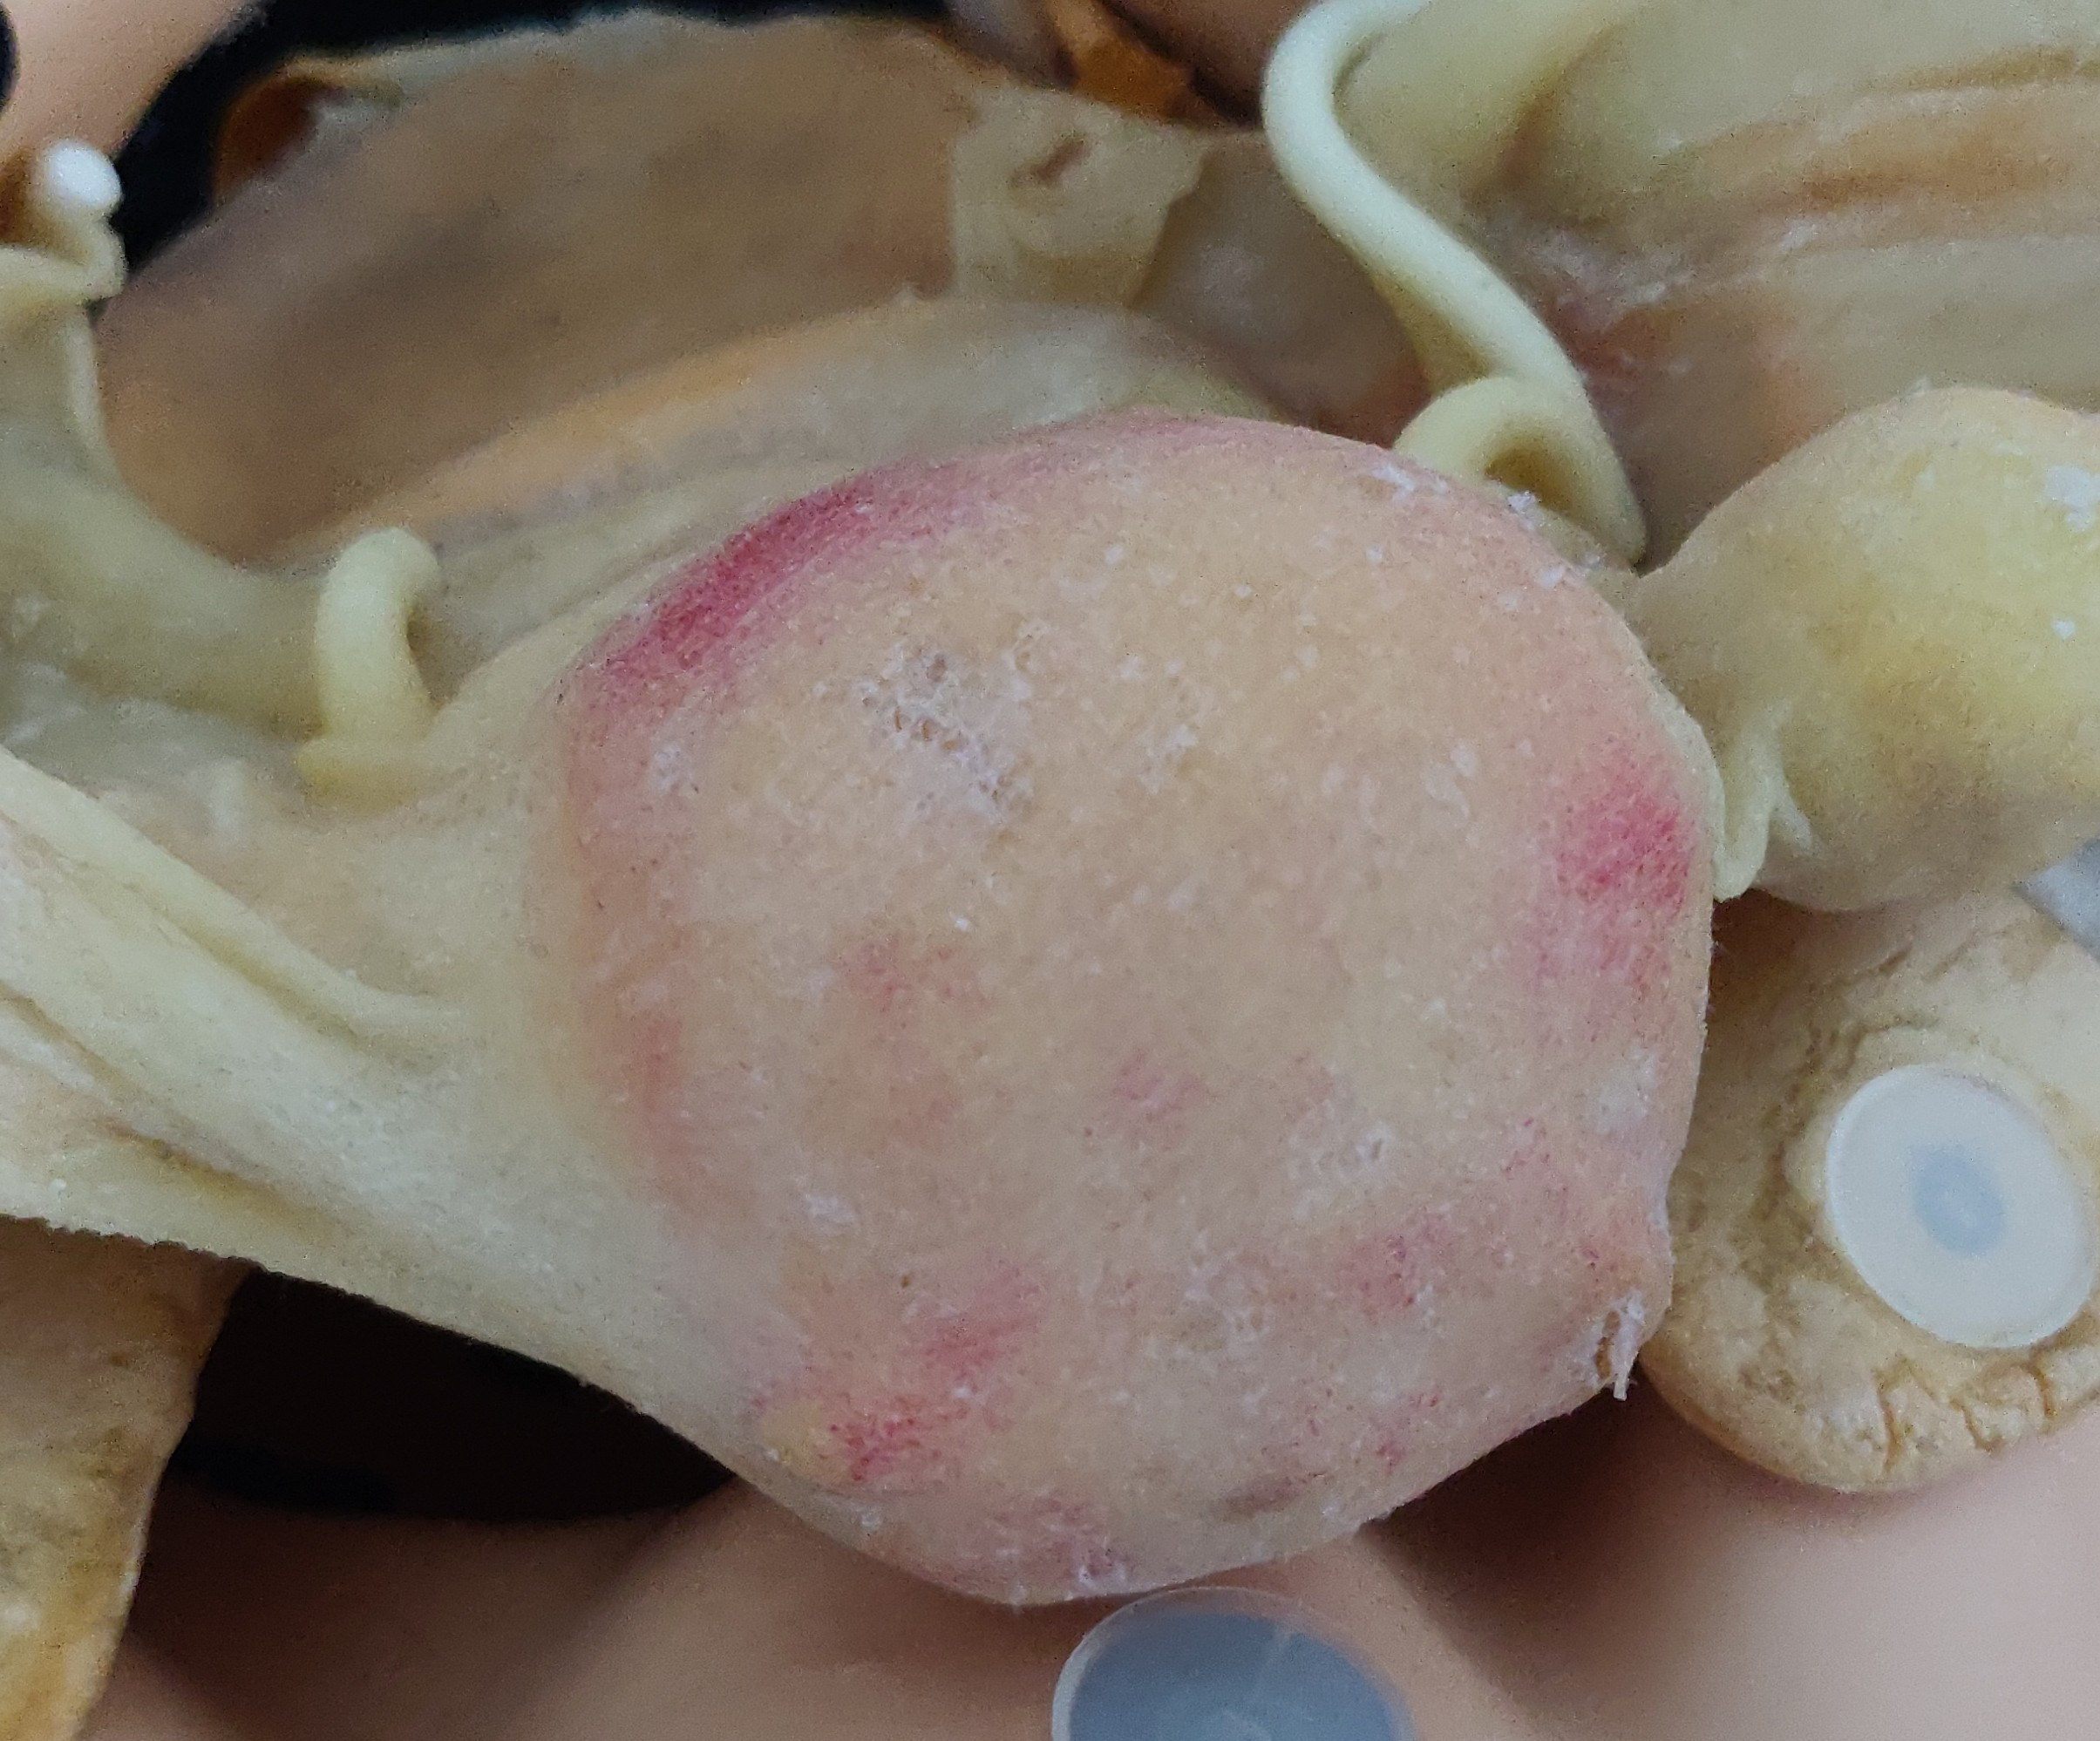
\includegraphics[width=0.4\columnwidth]{./figs/phantom.png}
  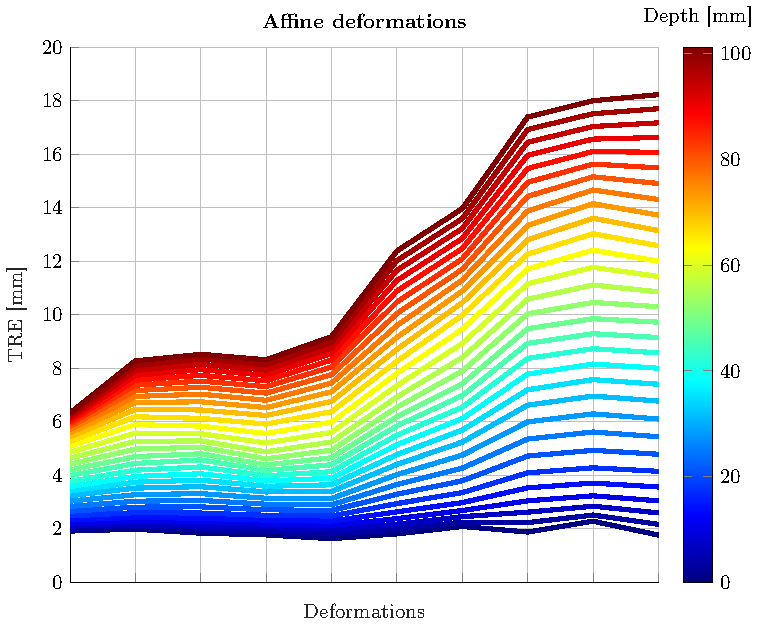
\includegraphics[width=0.49\columnwidth]{./figs/affineError.pdf}
  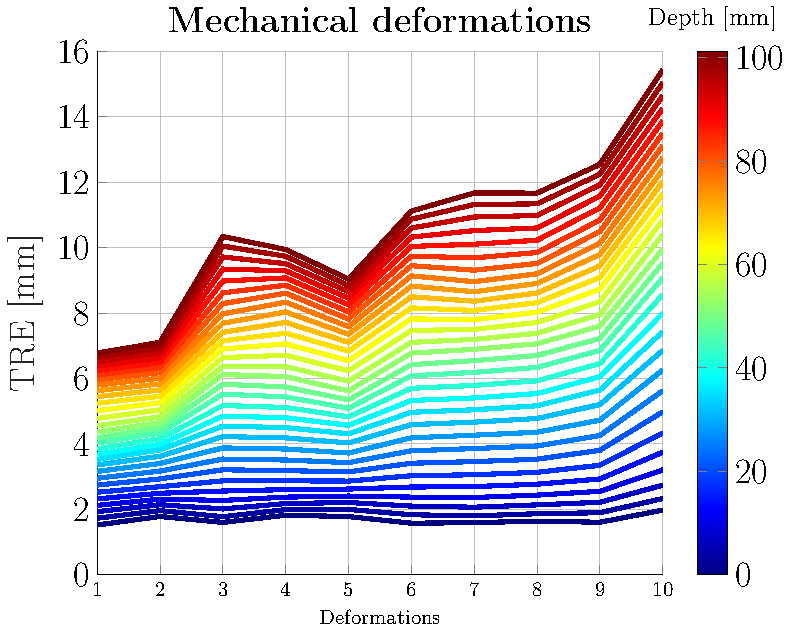
\includegraphics[width=0.49\columnwidth]{./figs/mechanicalError.pdf}
%  \includegraphics[width=0.4\columnwidth]{./figs/TRE_3Dmodels.pdf}
%  \caption{From left to right, the phantom used for the experiment, the TRE for the affine deformations and the mechanical deformations and the distribution of TRE on the surface of the 3D model.}
  \caption{TRE for affine (left) and mechanical (right) deformations. The deformation extent increases along the $x$-axis. The TRE is shown for different depths from the fundus.}
  \label{fig:TRE}
\end{figure}

\SGG{In our workshop paper~\cite{Collins2044} we presented a thorough evaluation of the initial registration step on a 3D printed uterus phantom and different synthetically deformed shapes.
%We synthetically deformed the CAD model to simulate a range of different pre-operative shapes of the uterus.
%To test the accuracy of the initial registration, we use an affine deformable model and we assessed the influence of the number of keyframes on the registration accuracy.
The results showed that the registration error decreases with the number of keyframes, and saturates approximately at \SI{1.4}{\milli\metre} for more than $8$ keyframes.
More generally, the error distribution tends to increase towards the cervix (\SI{2}{\milli\metre} for $15$ views up to \SI{8}{\milli\metre} for $2$ views) away from the uterus head as the uterus head is quite well constrained by the SfM point cloud as opposed to deeper regions near the cervix.
}

\SGG{In this section we present a new experiment to evaluate the Target Registration Error (TRE) of the the full registration pipeline (initial registration and tracking) with a realistic latex Phantom (Limbd and Things Inc. Model XX). We collected $\termName{N}{gt}=200$ images of the phantom, from which we computed a 3D surface model using MVS. We used this model as the pre-operative model, and we
%We then run our reconstruction pipeline on a subset of $\termName{N}{s}=15$ images.% and we scaled and aligned the obtained MVS model to the GT model to get a metric reconstruction in the same reference frame.
synthetically deformed it to simulate different preoperative states with two kinds of deformations: isovolumetric affine deformations, and mechanical deformations~\cite{Collins2044} that simulate bending of the organ using a quadratic deformation law along a principal axis. 
We generated $10$ examples of each, progressively increasing the amount of deformation magnitude. For each generated deformation $\Theta(\cdot)$, we apply our registration pipeline, using $\termName{N}{s}=15$ images for the initial registration step and $\termName{N}{gt}-\termName{N}{s}$ images for tracking.
%non-rigid registration with the MVS model and we ran our tracker on the remaining $\termName{N}{gt}-\termName{N}{s}$ images.
We discretize the GT volume with a grid of $100\times100\times100$ voxels and, denoting $\mathcal{V}$ the set of voxels in the interior of the uterus, we define the TRE for each grid point $\vet{q} \in \mathcal{V}$ for a given tracked image as $\| f( \Theta(\vet{q}),\mathbf{x}_t) -  \mat{P}_{\text{gt}}(\vet{q}) \|$, where $\vet{x}_t$ are the model registration parameters estimated by our pipeline and $\mat{P}_{\text{gt}}$ is the ground truth pose provided by the initial MVS reconstruction. TRE varies as a function of both the depth of the target and the amount of organ deformation. We visualize the trends in \fig{fig:TRE}.\fig{fig:TRE} shows TRE error in terms of \textit{i)} voxel depth and \textit{ii)} deformation magnitude. Voxel depth was computed as the Euclidean distance from each voxel to the visible head surface of the uterus. f the uterus ion for voxles different depths computed in mm from the  visble surface of the uterus. We report TRE averaged over all the tracked frames for voxels at 30 different depths from the fundus, ranging from 0 mm to 100 mm (approximately the cervix). 
TRE in the funhead of the uterus ranges from $\SI{1.8}{\milli\metre}$ to $\SI{2.1}{\milli\metre}$ for the most severe affine deformation.
The error increases towards the cervix, from $\SI{6.7}{\milli\metre}$ up to $\SI{15.6}{\milli\metre}$. The increase in TRE with depth from the uterus head is normal and expected because of the increasing distance from the visible surface. The low registration error indicates the pipeline is sufficiently accurate for AR guidance of structures in the uterus fundus region. 
}

%\subsection{Quantitative Evaluation with Simulation experiments}
%\label{sec:experiments_Simulation}
%
%We present an evaluation of our initial registration stage using a $90 \times 60 \times 60~\si{\cubic\milli\metre}$  3D printed rigid uterus phantom where its preoperative shape deformation is simulated in software.
%\fig{fig:phantom}(a)) shows the phantom body with a printed realistic texture extracted from images of a human uterus and placed inside a pelvic trainer (\fig{fig:phantom}(b)) to simulate the laparoscopic conditions.
%The exploratory video is taken with a $\SI{10}{\milli\metre}$ Karl Storz HD laparoscope fixed to the pelvic trainer through a flexible arm.
%To simulate the rotation of the cannula as in real surgery, we rotated the model about the cervix and we acquired $K=20$ keyframes (\fig{fig:reconstruction}).
%% We introduced the phantom into a pelvic trainer (\fig{fig:phantom}(b)) to simulate the laparoscopic conditions, using a $\SI{10}{\milli\metre}$ Karl Storz HD laparoscope fixed to the pelvic trainer through a flexible arm.
%% We performed the exploratory video by rotating the model about the cervix similarly to the motion experienced in real surgery by rotating the cannula, keeping $K=20$ keyframes (\fig{fig:reconstruction}).
%
%\begin{figure}[t]
%  \centering
%  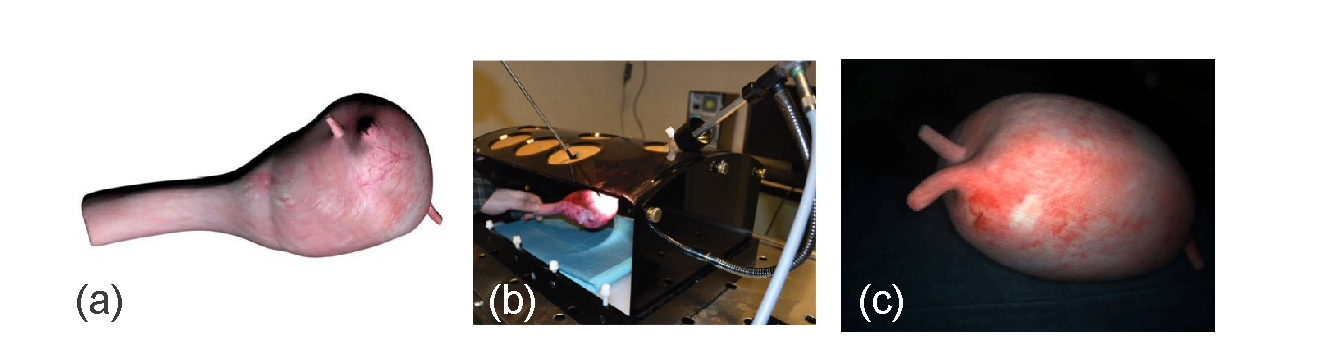
\includegraphics[width=0.5\textwidth]{./figs/phantom.pdf}
%\caption{(a) Uterus CAD model. (b) 3D printed phantom inside a pelvic trainer with a \SI{10}{\milli\metre} Karl Storz HD laparoscope. (c) Laparoscopic images of the phantom.}
%\label{fig:phantom}
%\end{figure}
%
%
%\begin{figure*}[htb]
%  \centering
%  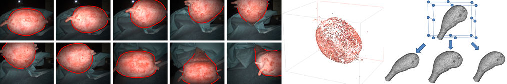
\includegraphics[width=0.9\textwidth]{./figs/markupWithDefSimCompressed.pdf}
%\caption{Left: Exploratory keyframes with occluding contour fragments. Middle: Sparse 3D cloud from SfM. Right: The grid of control points  with the 3D pre-operative model (up) and an example of the generated synthetic deformations (bottom).}
%\label{fig:reconstruction}
%\end{figure*}
%
%We synthetically deformed the CAD model to simulate a range of different pre-operative shapes of the uterus.
%We employed Thin-Plate Spline (TPS) to represent the volumetric deformation model.
%We uniformly sampled the CAD model with a grid of $2\times 3 \times 3$ control points.
%% To this end we used a volumetric deformation model represented with the Thin-Plate Spline (TPS).
%% The TPS was defined by a set of $2\times 3 \times 3$ control points uniformly spaced over the CAD model.
%\fig{fig:reconstruction} shows the non-linear volumetric deformations that we could generate by perturbing the control point set.
%% By perturbing the control point grid we could create non-linear volumetric deformations (see \fig{fig:reconstruction}, right).
%This enabled us to create many pre-operative deformations: first the reference control points were transformed with a random global affine transformation and then they underwent a random displacement of standard deviation $\sigma_p=\SI{10}{\milli\metre}$.
%% We generated many pre-operative deformations first applying a random global affine transform to the reference control points followed by a random displacement of standard deviation $\sigma_p=\SI{10}{\milli\metre}$.
%We define the TPS as $\wTPS(\cdot,\thetaTPS)$, where $\thetaTPS$ holds the control centers (\ie $18\times 3$ parameters in total).
%
%%
%%\begin{figure}[htb]
%  %\centering
%  %\includegraphics[width=0.3\textwidth]{./figsSimulation/deformSimulation.pdf}
%%\caption{Up: Intra-operative phantom surface, overlaid with the TPS grid of control points. Down: Several synthetic deformations obtained with the TPS.}
%%\label{fig:uterusDeformations}
%%\end{figure}
%To test the accuracy of the initial registration, we use an affine deformable model.
%This was chosen because the synthetic deformation we induce with the TPS model cannot be exactly approximated by the deformation model.
%We used this to test our system's robustness to unmodelled deformation modes, which likely occur when dealing in real conditions with real deformations.
%To assess the influence of the number of keyframes on the registration accuracy, we randomly selected sets of $\{2,3,4,5,6,7,10,15\}$ images from the initial $K=20$ keyframes.
%For each of them we generated $50$ random deformations with the TPS.
%% Our quantitative experiment tested the influence of the number of keyframes on the registration accuracy. We randomly selected sets of $\{2,3,4,5,6,7,10,15\}$ images from the $K=20$ keyframes. For each set we generated $50$ random deformations with the TPS.
%\fig{fig:results}(a) shows the marked contours from $3$ different keyframe overlaid with the shape of three deformed models.
%We measured registration error in 3D by discretizing the internal volume of the uterus model with a grid of $100\times 100 \times 100$ voxels. We defined the registration error $\epsilon_r$ as follows:
%%\begin{figure}[htb]
%%  \centering
%%  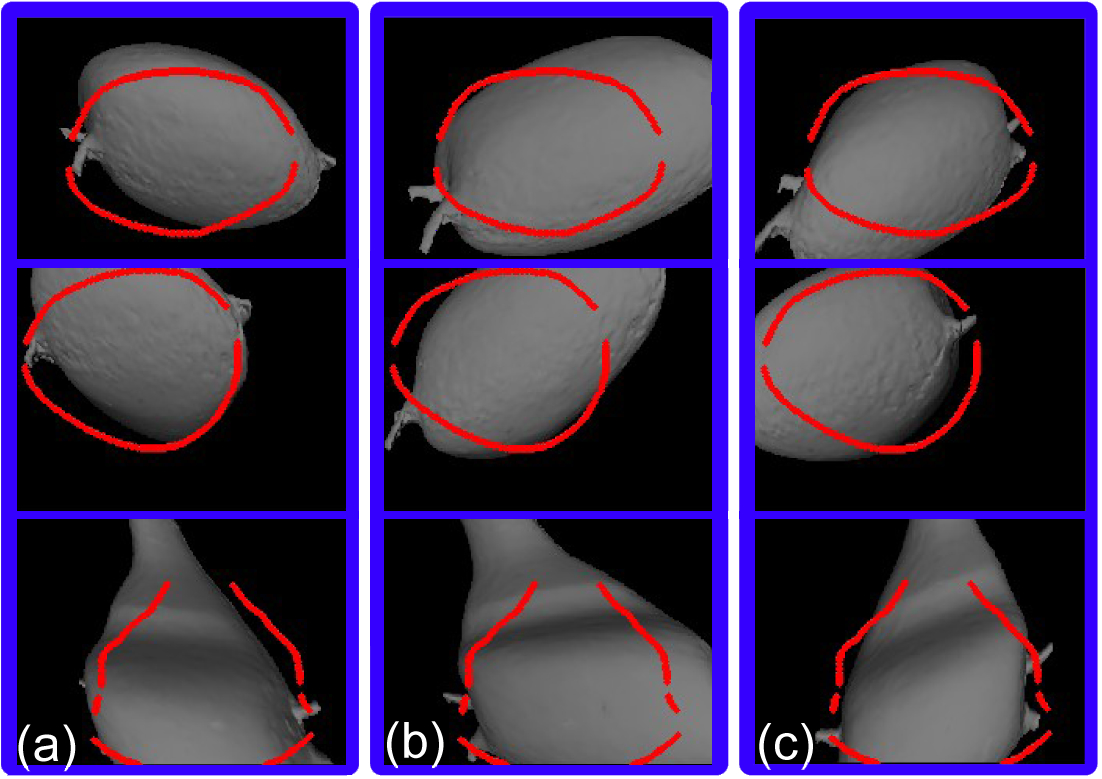
\includegraphics[width=0.35\textwidth]{./figs/initial_.pdf}
%%\caption{(a), (b) and (c) show the initial projection of three different pre-operative models (one model per column) in three different views (one view per row) using the $z$-buffer. We overlay on top the contours from each view given by the user.}
%%\label{fig:InitialSolutions}
%%\end{figure}
%\begin{figure*}[htbp]
%  \centering
%  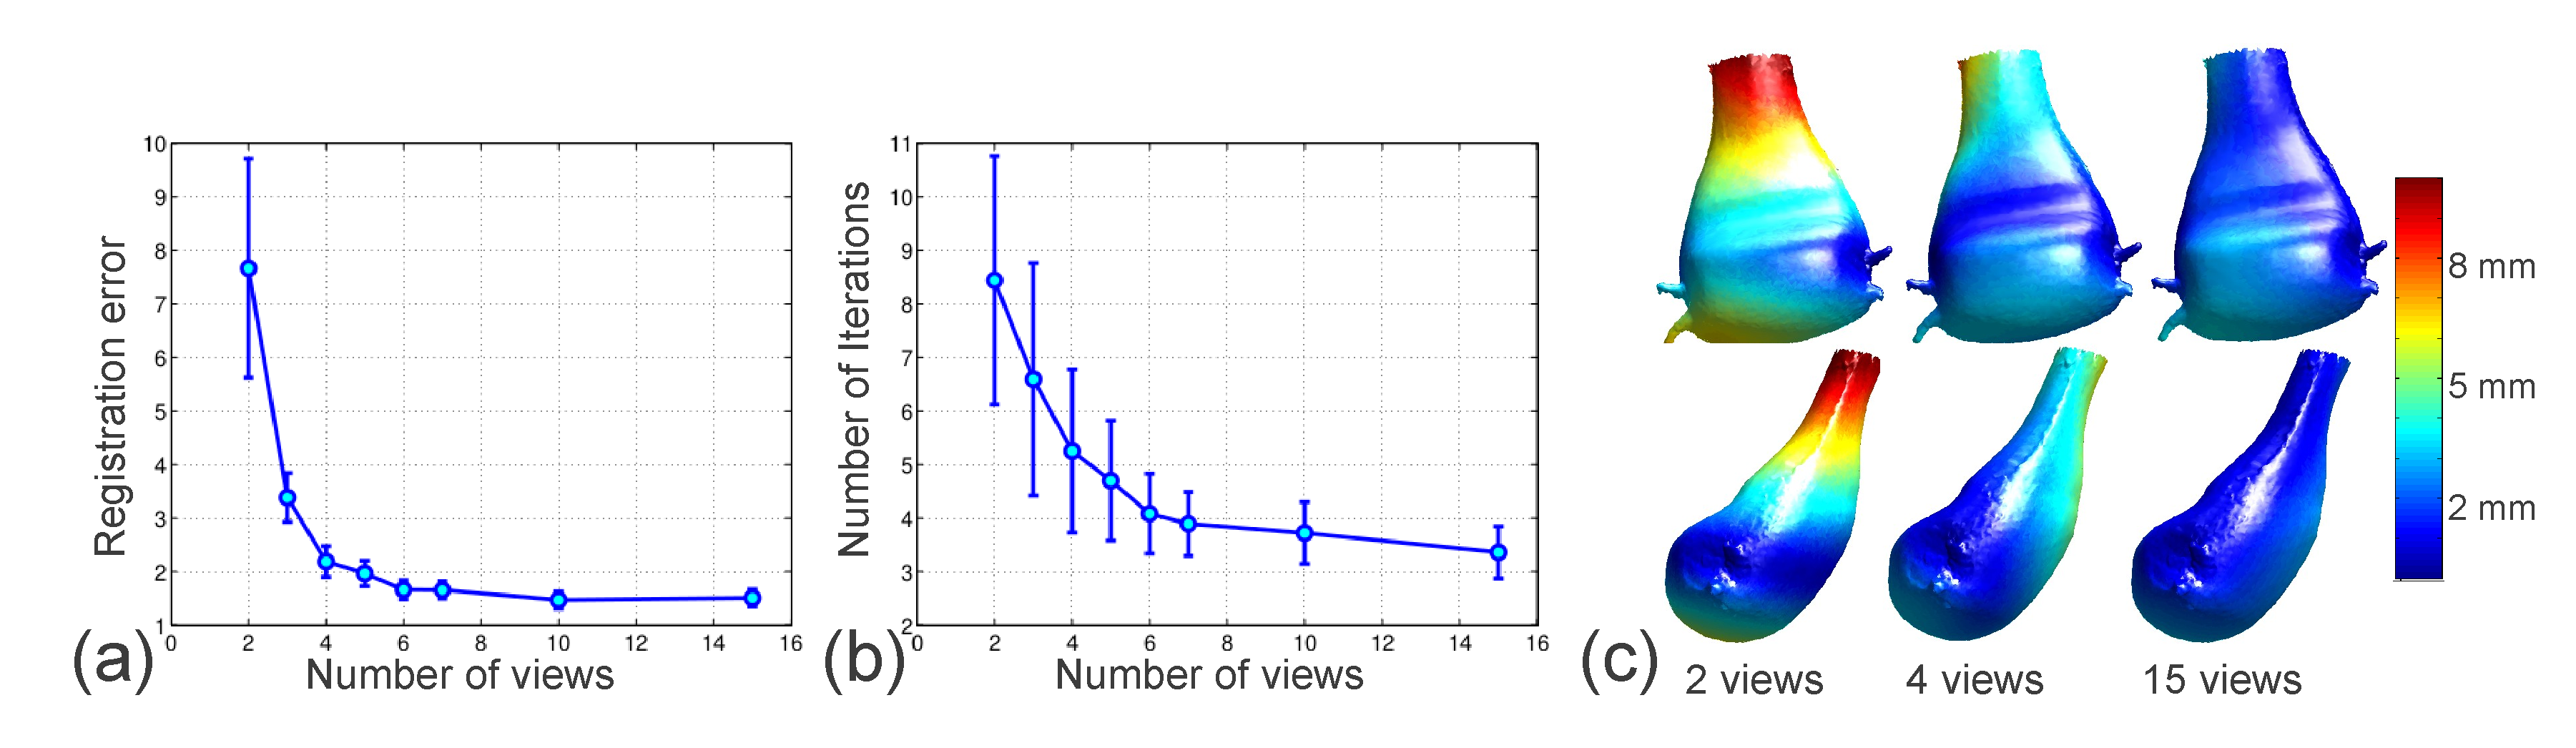
\includegraphics[width=0.95\textwidth]{./figs/errors.pdf}
%\caption{(a) Each column shows the initial projection of a different pre-operative model in $3$ views (one per row). The red curves show the contours marked by the user. (b) Registration error vs. number of views. (c) Number of iterations vs. number of views. (d) Mean surface registration error for $2$, $4$ and $15$ views.}
%\label{fig:results}
%\end{figure*}
%
%\begin{equation}
%  \label{eq:regerror}
%  \epsilon^2_r=\frac{1}{N_{\mathcal{V}}}\sum_{\mathbf{q}\in \mathcal{V}} \|f(\wTPS(\mathbf{q};\thetaTPS),t_0;\theta)-\mathbf{q}\|^2,
%\end{equation}
%where $\mathcal{V}$ is the set of voxels in the interior of the uterus volume.
%We report in \fig{fig:results}(b) the mean registration error as a function of the number of the available keyframes.
%In \fig{fig:results}(c) we show the mean number of iterations our method requires to reach convergence.
%% \fig{fig:results}(b) shows the mean registration error as a function of the number of available keyframes. \fig{fig:results}(c) shows the mean number of iterations our method requires to reach convergence.
%\fig{fig:results}(d) shows the distribution of registration error over the uterus surface using a heatmap. The registration error clearly decreases with the number of views, and saturates approximately at \SI{1.4}{\milli\metre} for more than $8$ views. With $2$ views the registration error distribution in \fig{fig:results}(d) tends to increase towards the cervix, away from the uterus head. This makes sense as the uterus head is quite well constrained by the SfM pointcloud as opposed to the area near the cervix.
%By contrast, with more views we have more constraints from the silhouette contours, as these reveal the boundaries of the uterus from a greater range of viewpoints, and the result is a significant improvement in registration. This experiment provides strong evidence for the value in using multiple viewpoints to constrain the registration problem, compared with prior works that uses only one viewpoint. In addition we that more views significantly reduce the number of iterations required for convergence.

\subsection{Evaluation with Human Uteri in Pre-recorded Videos}
\label{sec:orbslam}
In this section we present results on videos recorded during laparoscopic surgery.
We test accuracy, computational complexity and the influence of the keypoint detector in our real-time organ tracking by detection system, named RT-OTD in the experiments.
\SGG{We demonstrate the robustness of our model-based approach \wrt classic SLAM approaches~\cite{orbslam_laparo} and we show augmentation results, completing the AR pipeline}
%We compare it with ORB-SLAM, state-of-the-art for SLAM-based tracking in laparoscopic videos~\cite{orbslam_laparo}.
%We show augmentation results, completing the AR pipeline.


\subsubsection{Automatic Keyframe Selection for 3D Reconstruction}
\label{subsec:automatic-keyframe-selection}
\SG{We compare the automatic keyframe selection method \emph{auto} to results obtained by sampling the exploratory video ($\sim \SI{60}{\second}$) to obtain the $15$ keyframes, with different sampling methods: \emph{equally} samples the video uniformly, \emph{beginning}, \emph{middle} and \emph{end} take a keyframe every $t=\SI{2}{\second}$ from the beginning, around the middle and towards the end of the video, respectively.
We then proceed with reconstruction and tracking for each strategy.
\fig{fig:3DresultsKframeSelection} shows the 3D models.
Qualitatively, \emph{auto} gave a better model as all the others have many holes.
This is explained by 1) some selected keyframes are blurry and 2) there are many similar keyframes, thus preventing a complete coverage of the full organ shape.}

\SG{We recorded another video ($\sim \SI{60}{\second}$) in order to test the tracking  using the 3D models obtained from each method.
The video was purposely challenging, with the camera looking at parts of the uterus that were not completely reconstructed in any of the models, and no additional keyframes added during tracking.
\emph{auto} was able to track the largest number of frames ($\SI{55.18}{\percent}$), followed by \emph{equally} ($\SI{53.33}{\percent}$), \emph{middle} ($\SI{52.48}{\percent}$), \emph{beginning} ($\SI{46.14}{\percent}$) and \emph{end} ($\SI{31.08}{\percent}$).
\fig{fig:statsKframeSelection} reports tracking statistics.
In general, \emph{auto} recovers a larger number of valid matches, both \wrt all the keyframes in the database (\fig{fig:statsKframeSelection}.a) and the winning keyframe (\fig{fig:statsKframeSelection}.b) and computes the pose with a larger number of inliers.
The reprojection error is also slightly better than all the other methods, especially considering the higher number of inliers over which it is computed.
Overall, automatic keyframe selection improves the quality of reconstruction and tracking.
Any sampling method is always potentially affected by motion blur; guiding the acquisition of the keyframe reduces the risk.}
%$\SI{46.14}{\percent}$ $\SI{52.48}{\percent}$ $\SI{31.08}{\percent}$ $\SI{53.33}{\percent}$ $\SI{55.18}{\percent}$

\subsubsection{Comparison of Different Tracking Keypoints}
\label{sec:siftvssurf}
%In this section we analyse the benefits of using SIFT features over SURF within the tracking stage. %SIFT features offer, in general, a more reliable and robust choice for feature matching but the major limitation is its computational time, which often prevents them from being used in real-time applications.
%We used a SIFT GPU implementation~\cite{Griwodz2018Popsift} which provides real-time performances with full HD images.
We tested our tracking method RT-OTD using PopSift~\cite{Griwodz2018Popsift} and the SURF-GPU from OpenCV on two videos.  
\begin{table}[]
\centering
\begin{tabular}{rlcccc}
\multicolumn{1}{c}{\# frames}              & \multicolumn{1}{c}{} & \# poses & \# matches & \begin{tabular}[c]{@{}c@{}}\# matches \\ winner\end{tabular} & \# inliers                 \\ \hline \hline
\multicolumn{1}{|r}{\multirow{2}{*}{$5000$}} & SURF                 & $4569$     & $406.16$     & $46.94 $                                                       & \multicolumn{1}{c|}{$32.93$} \\
\multicolumn{1}{|r}{}                      & SIFT                 & $4975$     & $388.06$     & $52.31$                                                        & \multicolumn{1}{c|}{$44.86$} \\ \hline
\multicolumn{1}{|r}{\multirow{2}{*}{$3029$}} & SURF                 & $2713$     & $296.81$     & $42.60$                                                        & \multicolumn{1}{c|}{$27.74$} \\
\multicolumn{1}{|r}{}                      & SIFT                 & $3029$     & $294.00$     & $64.87$                                                        & \multicolumn{1}{c|}{$52.81$} \\ \hline
\end{tabular}
\caption{Comparison in number of poses and matches between SIFT and SURF for two videos.}
\label{tab:matches}
\vspace{-2mm}
\end{table}
We see from \tab{tab:matches} that RT-OTD using SIFT establishes more camera poses (\SI{99.5}{\percent} and \SI{100}{\percent} of the frames) compared to SURF (\SI{91.2}{\percent} and \SI{89.6}{\percent}).
Despite the fact that SURF recovers, on average, more matches between $\mathcal{F}$ and $\mathcal{G}$, SIFT has a higher discriminative power in selecting the winning keyframe $i^*$.
As the table shows, the winning keyframe has, on average, more available matches from which RANSAC can sample to compute pose.
This also results in more inliers found to support the computed pose.
\begin{figure}[t]
  \centering
%  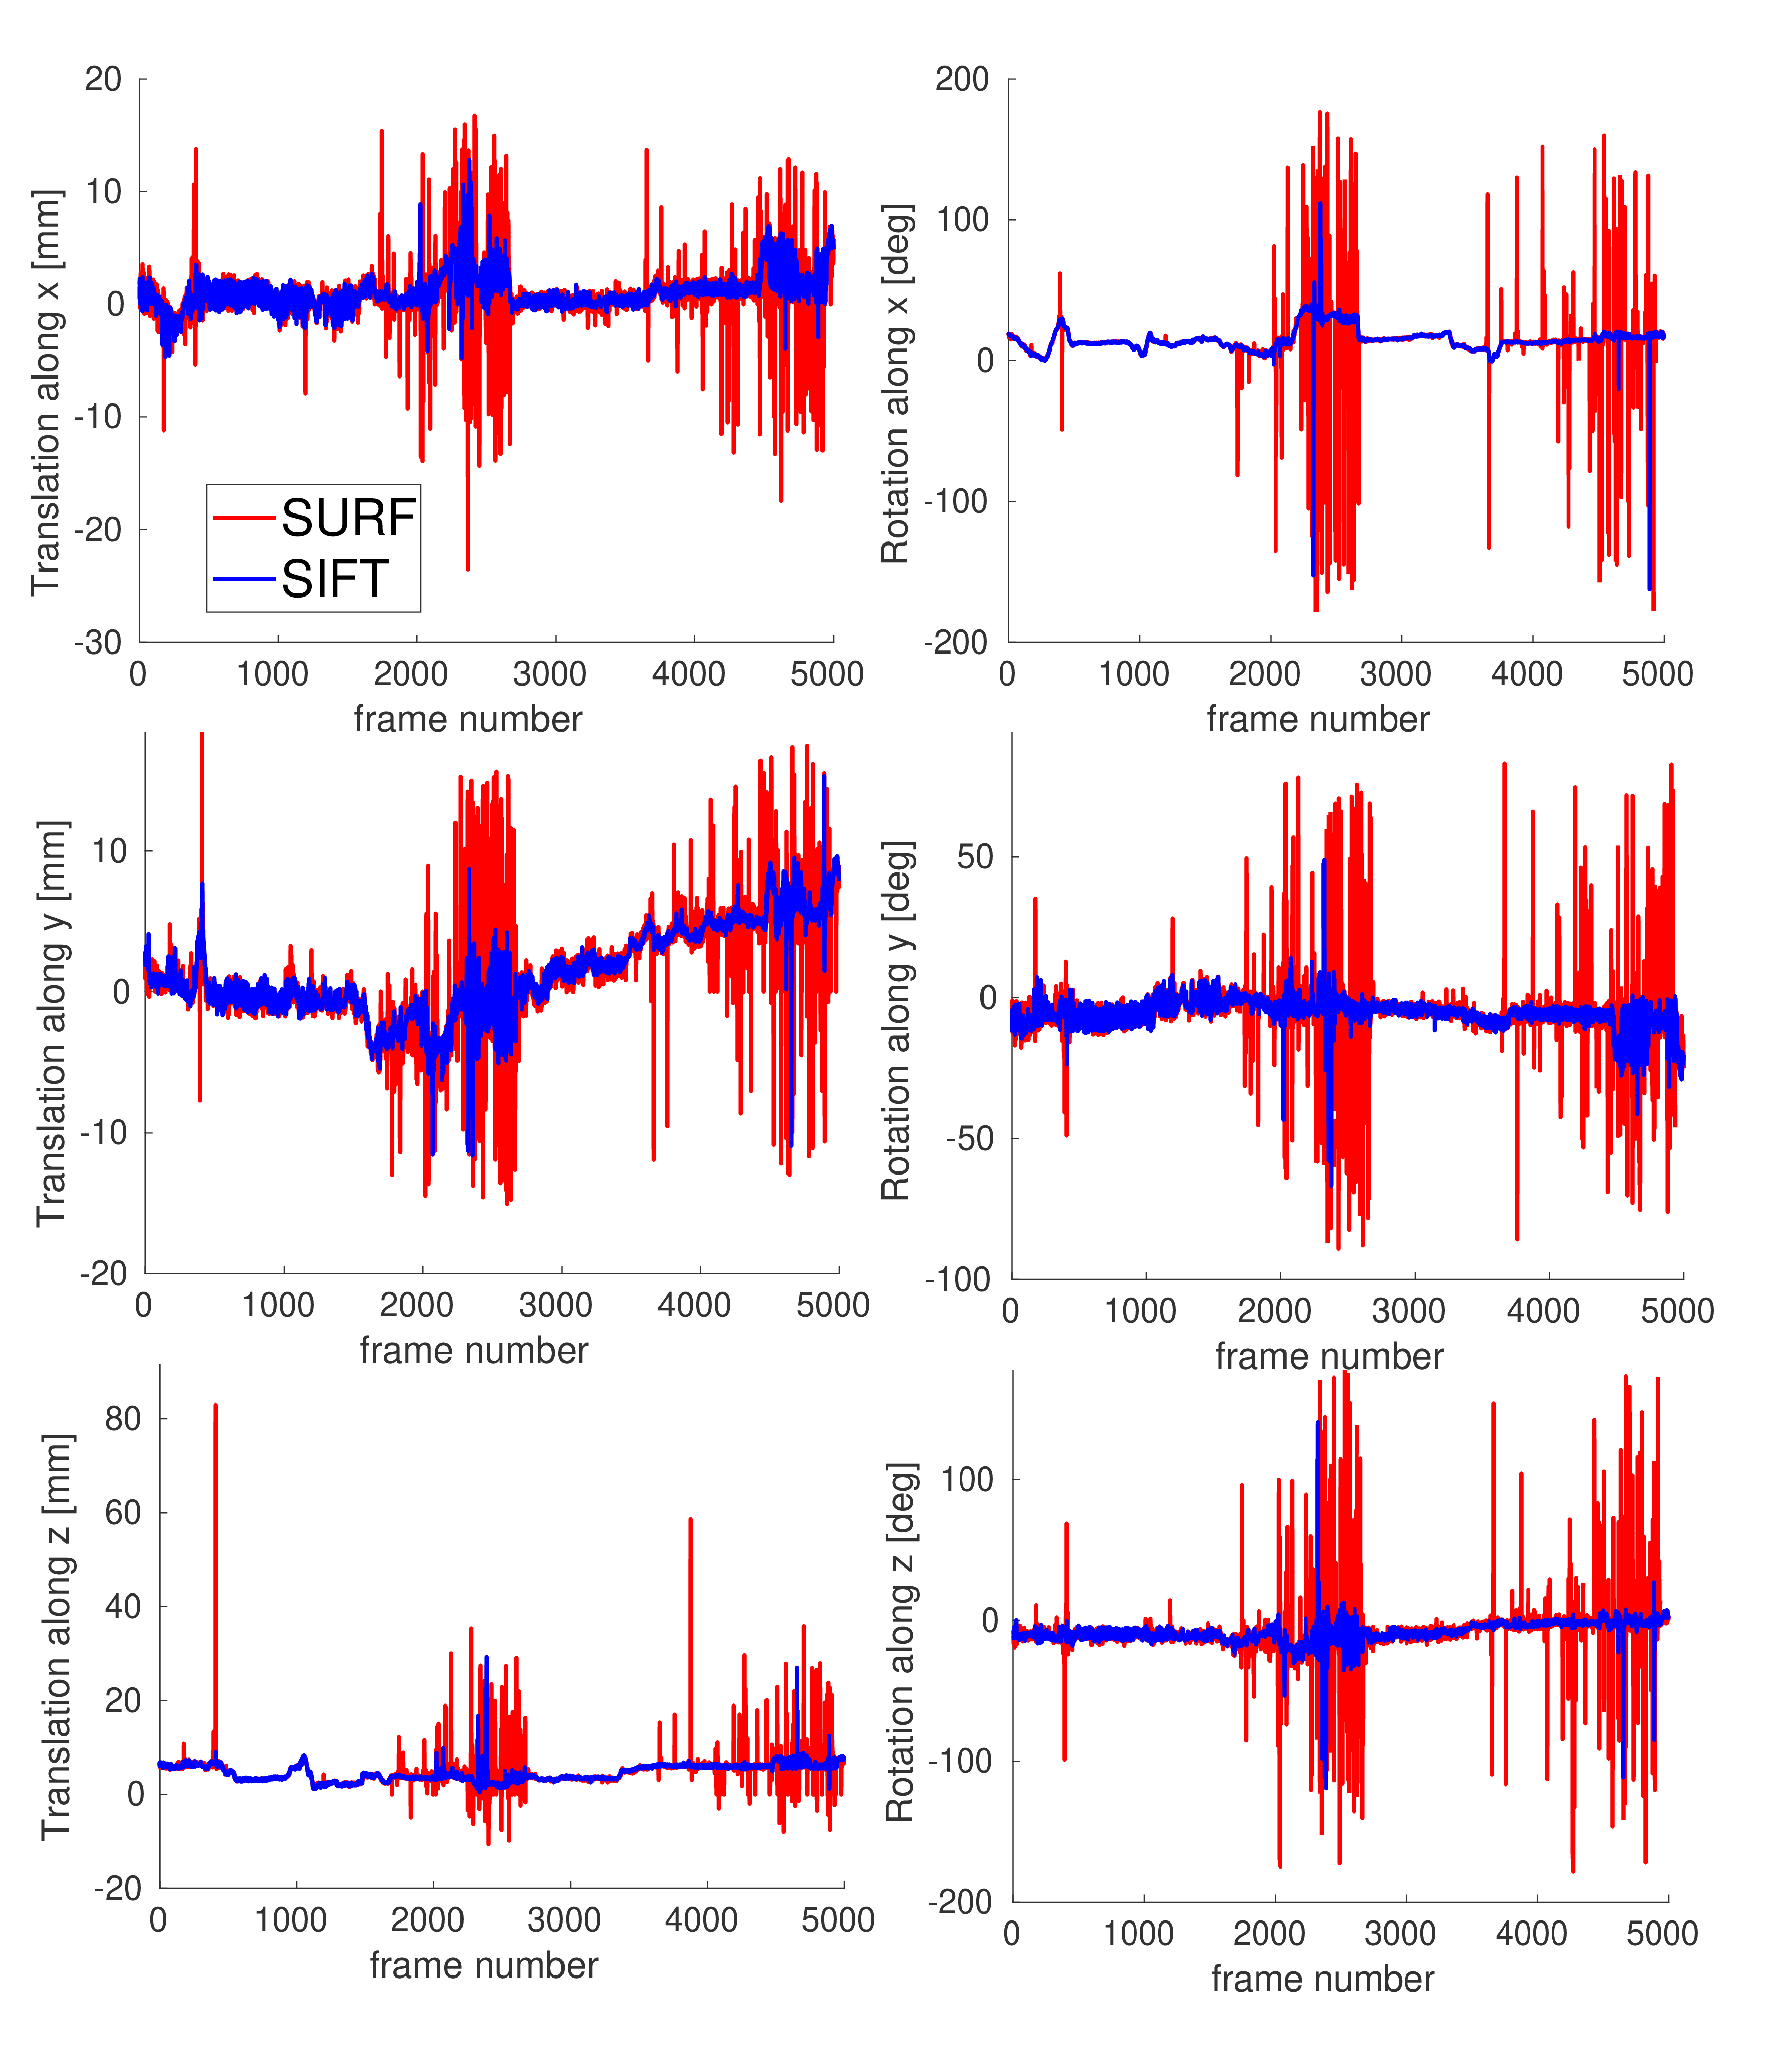
\includegraphics[width=0.4\textwidth]{./figs/Stability_Features.pdf}
  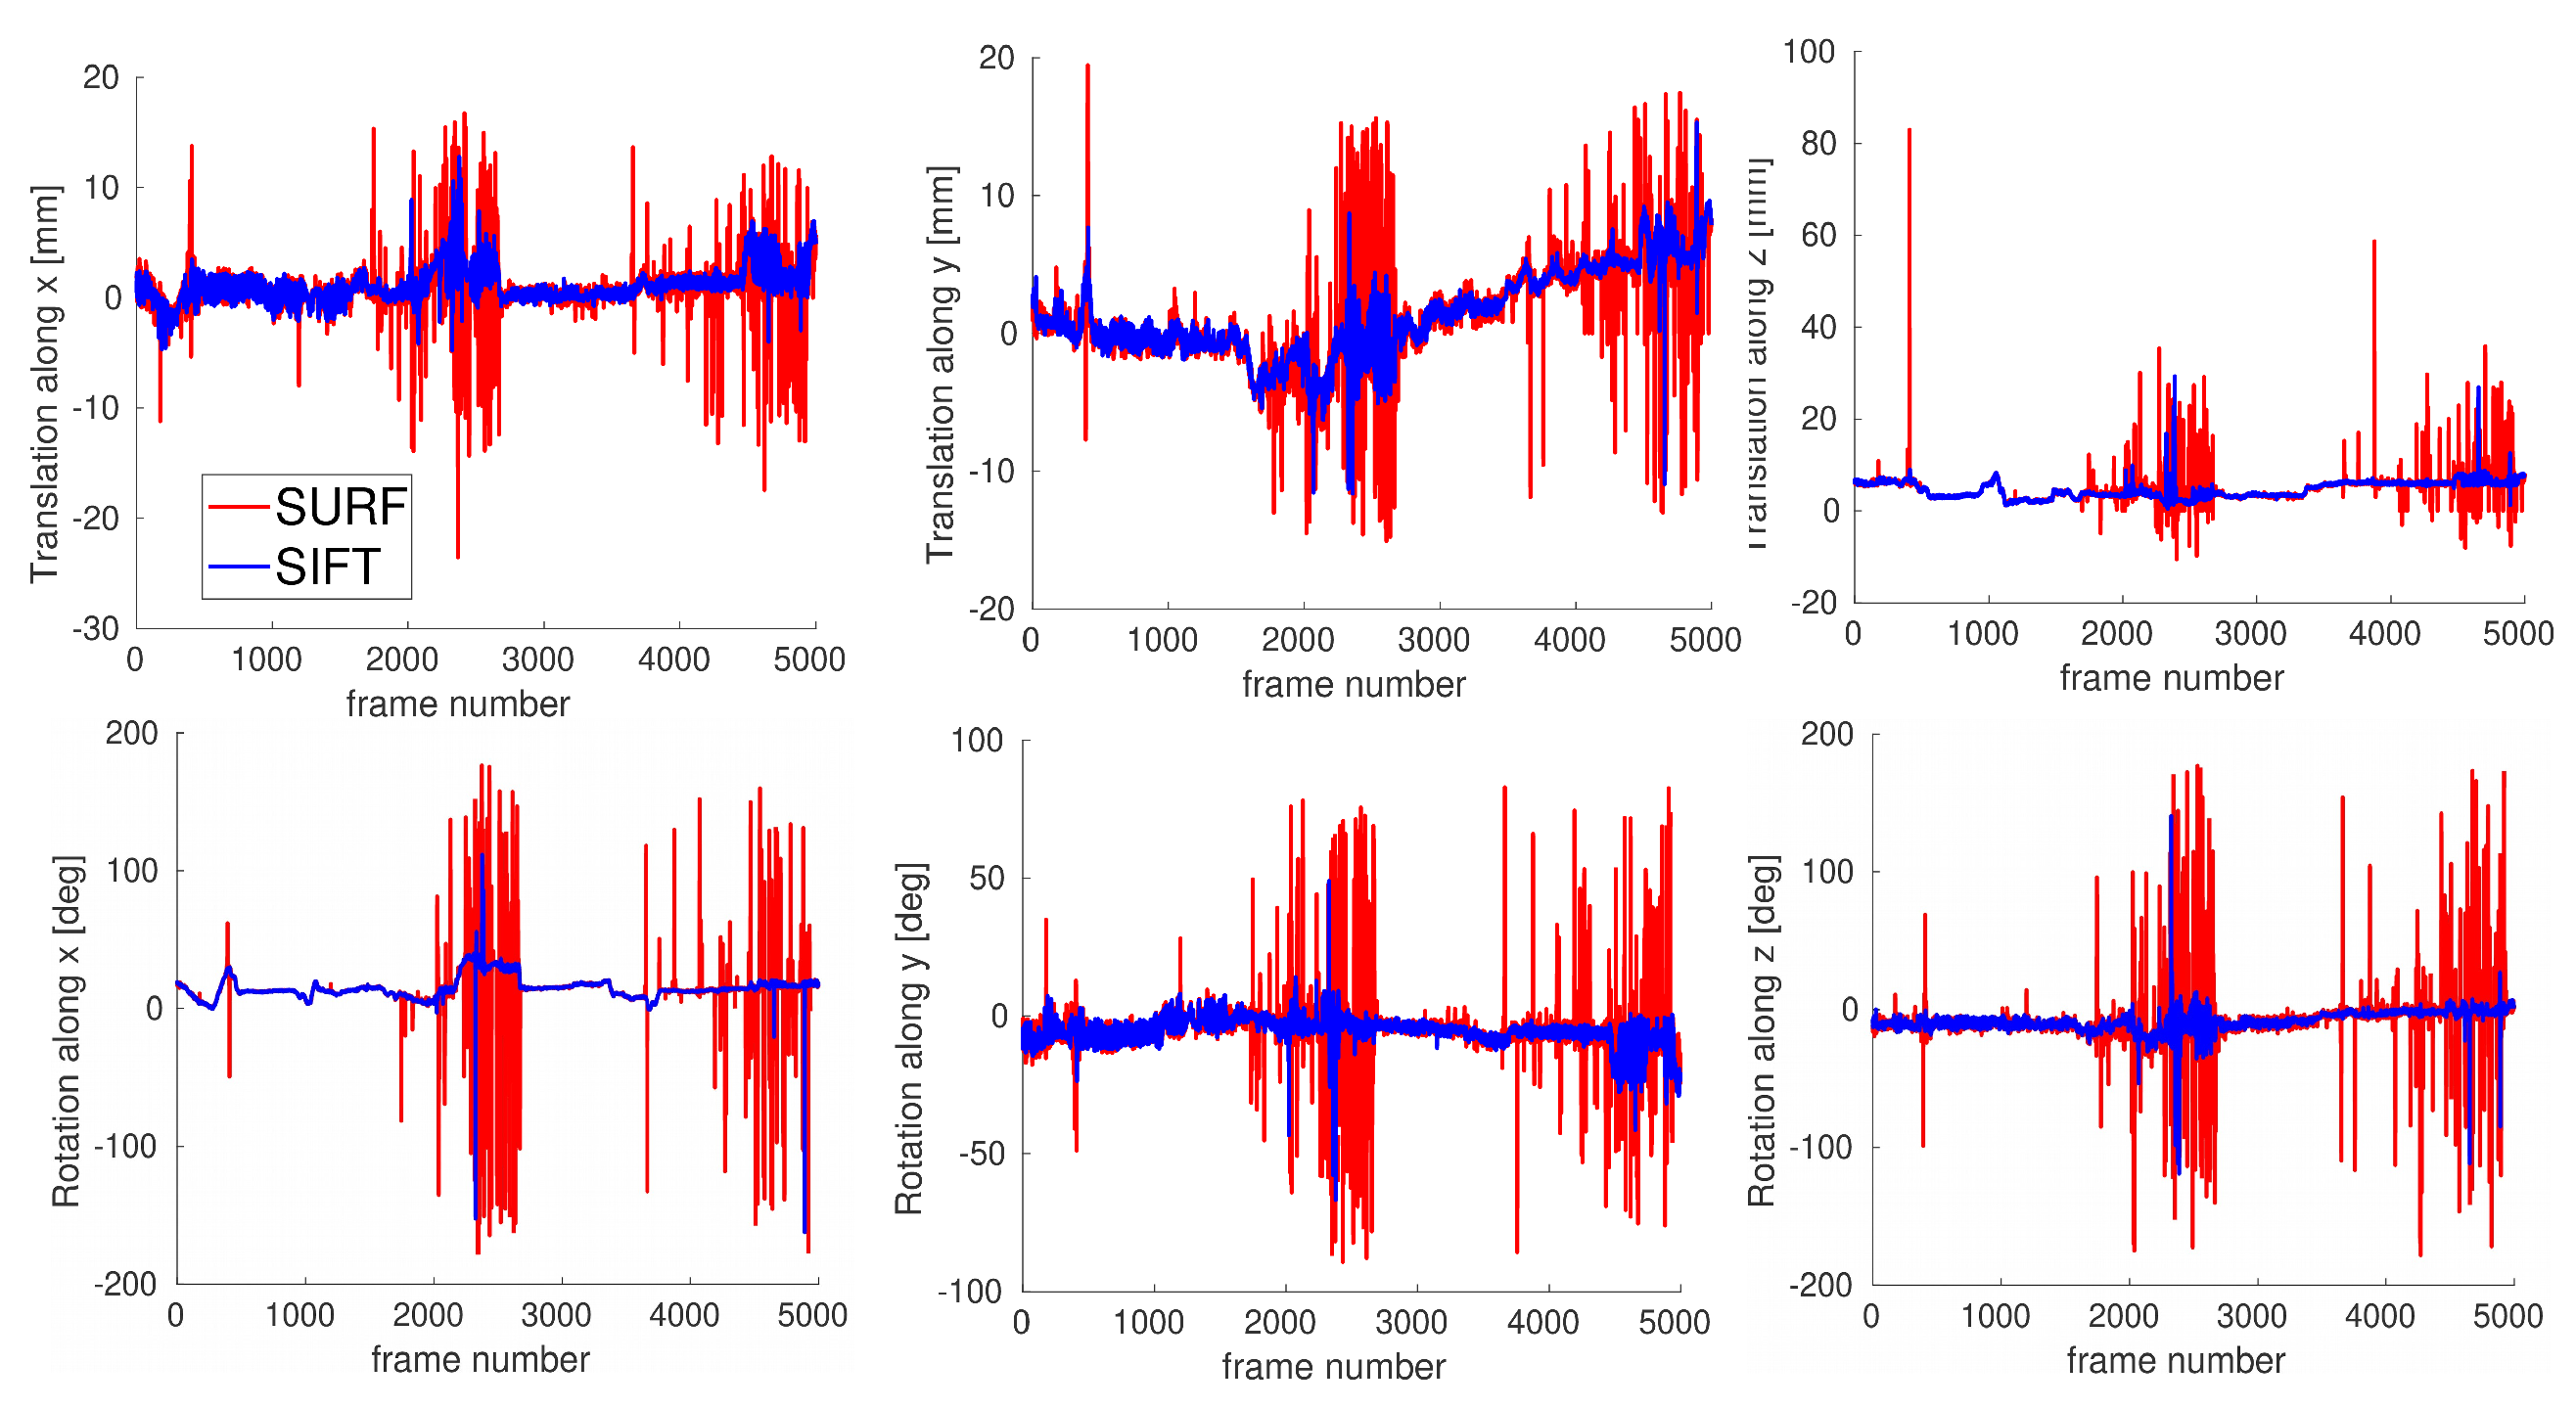
\includegraphics[width=0.45\textwidth]{./figs/Stability_Features2.pdf}
\caption{Comparing SURF and SIFT on $5000$ video frames.}
\label{fig:SurfVsSift}
\vspace{-5mm}
\end{figure}

\begin{figure}[ht]
  \centering
%  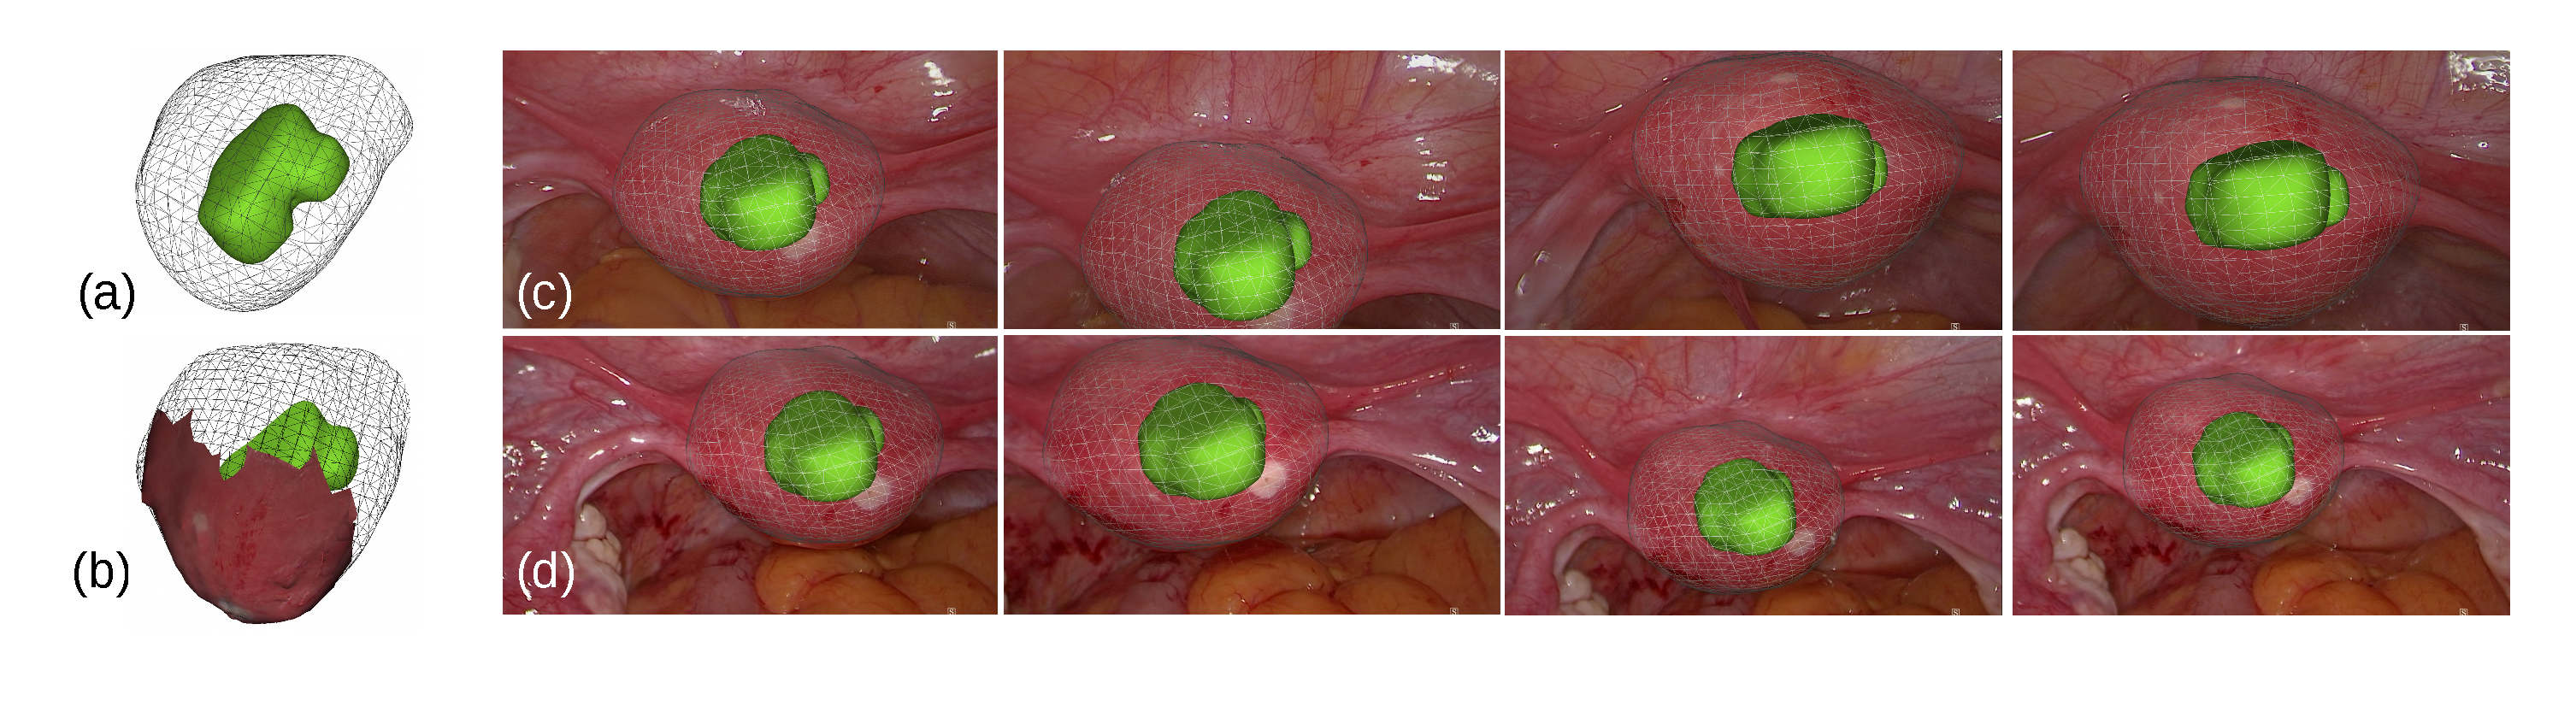
\includegraphics[width=0.835\textwidth]{./figs/frames_aug_new.pdf}
  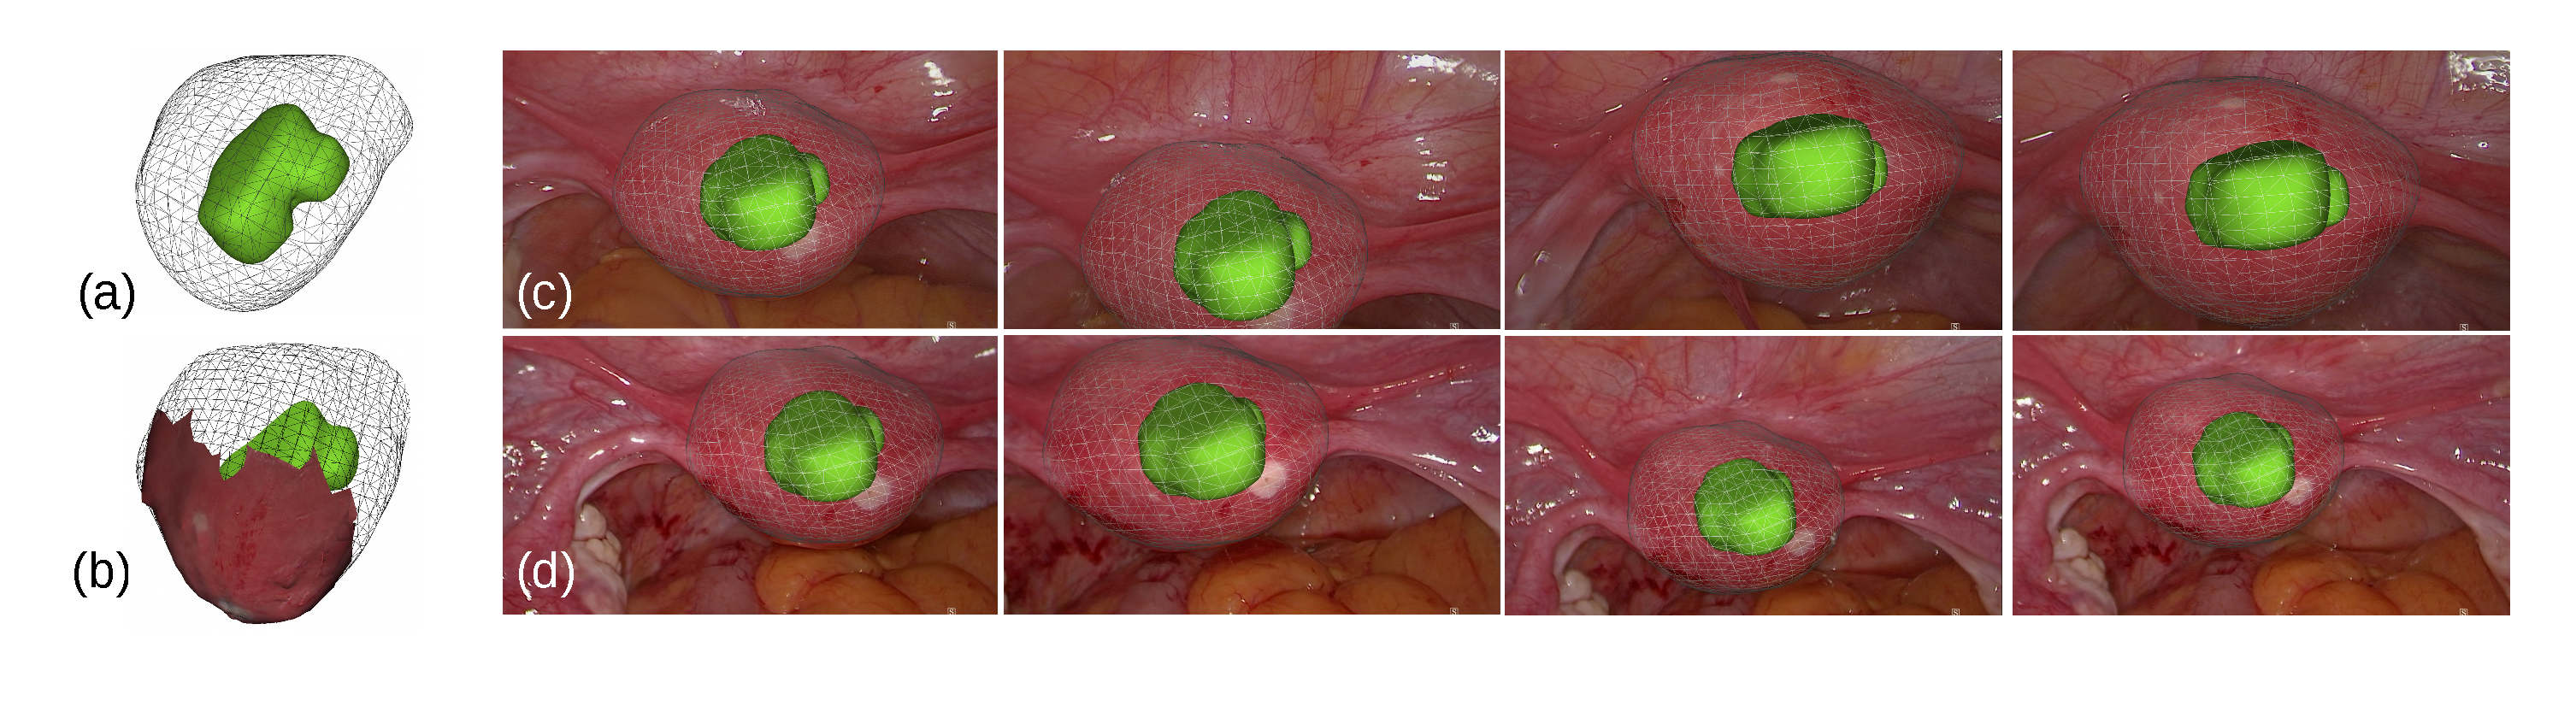
\includegraphics[width=0.99\columnwidth]{./figs/frames_aug_new.pdf}
\caption{(a) The 3D preoperative model of the uterus with the  myoma as reconstructed from the MR, (b) the preoperative model registered with the intraoperative model obtained from the MVS reconstruction (c) some of the keyframes used for MVS with the AR augmentation  (d) some frames of the video with the myoma shown as image overlay.}
\label{fig:myomas}
\vspace{-5mm}
\end{figure}
\begin{figure*}[ht]
  \centering
  \includegraphics[width=0.71\textwidth]{./figs/ARinOR.pdf}
\caption{Patient 1: (a) MR image showing one myoma, (b) myoma augmentation, (c) resection of the myoma, (d) deployment of our AR system in the OR. Patient 2: (e) MR image showing three myomas, (f,g,h) myoma augmentation. Patient 3: (i) two myomas segmented from the MR images, (j,k,m) augmentation of the myomas and the uterine cavity.}
\label{fig:realOR}
\end{figure*}

%\fig{fig:numMatches} shows the numbers of matches and inliers for both approaches for the first video sequence, where we see that all along the frames the number of matches used for computing the pose are always higher for SIFT. 
%In order to evaluate the quality of the estimated poses, 
We show both pose components in \fig{fig:SurfVsSift} for the $5000$ frame video.
SIFT provides a more stable estimate for both as there are much fewer spikes in the estimates (spikes are typically incorrect estimates).
This translates to a more stable motion estimate, improving overall AR quality with SIFT\@.
% The increased stability requires also less new keyframes to be added, thus, in turn, improving the overall computational time as less descriptor comparisons are needed.
The two videos and further results are shown in the video material. 

%\subsubsection{Tracking Accuracy and Comparison with ORB-SLAM}
\subsubsection{Tracking Accuracy and Comparison with SLAM}
We evaluate our tracking stage using three human uteri captured before hysterectomy.
They can be seen in \fig{fig:hister} and we refer to them as $U_1$, $U_2$ and $U_3$.
\begin{figure}[htb]
  \centering
  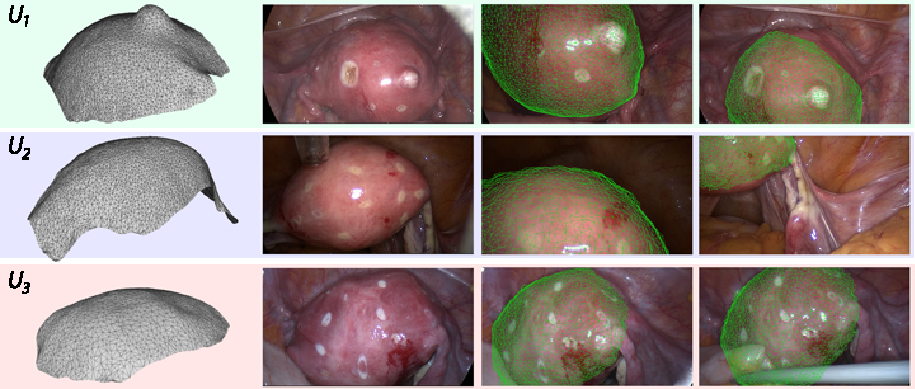
\includegraphics[width=0.4\textwidth]{./figs/snapshotsCompressed.pdf}
\caption{The 3D models from MVS, the coagulation marks and the registered models.}
\label{fig:hister}
\vspace{-5mm}
\end{figure}
Each video includes around $500$ frames showing image motion of the uterus due to motion induced by the cannula and camera motion.
The uterus intraoperative surface is obtained with an exploratory video with $15$ keyframes.
The uterus body was marked by the surgeon with a bipolar grasper in $12-15$ different locations.
% To obtain Ground-Truth (GT) camera pose the surgeon marked the uterus with a coagulation instrument at $12-15$  locations over the uterus body. 
This enabled us to generate Ground-Truth (GT) camera poses by tracking the obtained set of small marked regions ($\sim\SI{3}{\milli\metre}$ in diameter).
% This produced a set of small regions approximately $\SI{3}{\milli\metre}$ in diameter which could be accurately tracked. 
We show examples of these markers in \fig{fig:hister}. 
The marks were tracked using a small patch surrounding the image position of each marker, and fitted using a 2D affine transform. 
We verified all tracks and reinitialized them if they were lost.
We then computed the marks' 3D positions and the uterus 3D poses in each frame using SfM\@.
If fewer than four marks were visible in a frame we considered that the GT pose could not be estimated for that frame.
We masked each mark so that the methods under comparison could not exploit the artificial texture each mark introduces. 
We computed the optimal scale factor for each method \wrt GT\@.
\begin{figure}[!htbp]
  \centering
  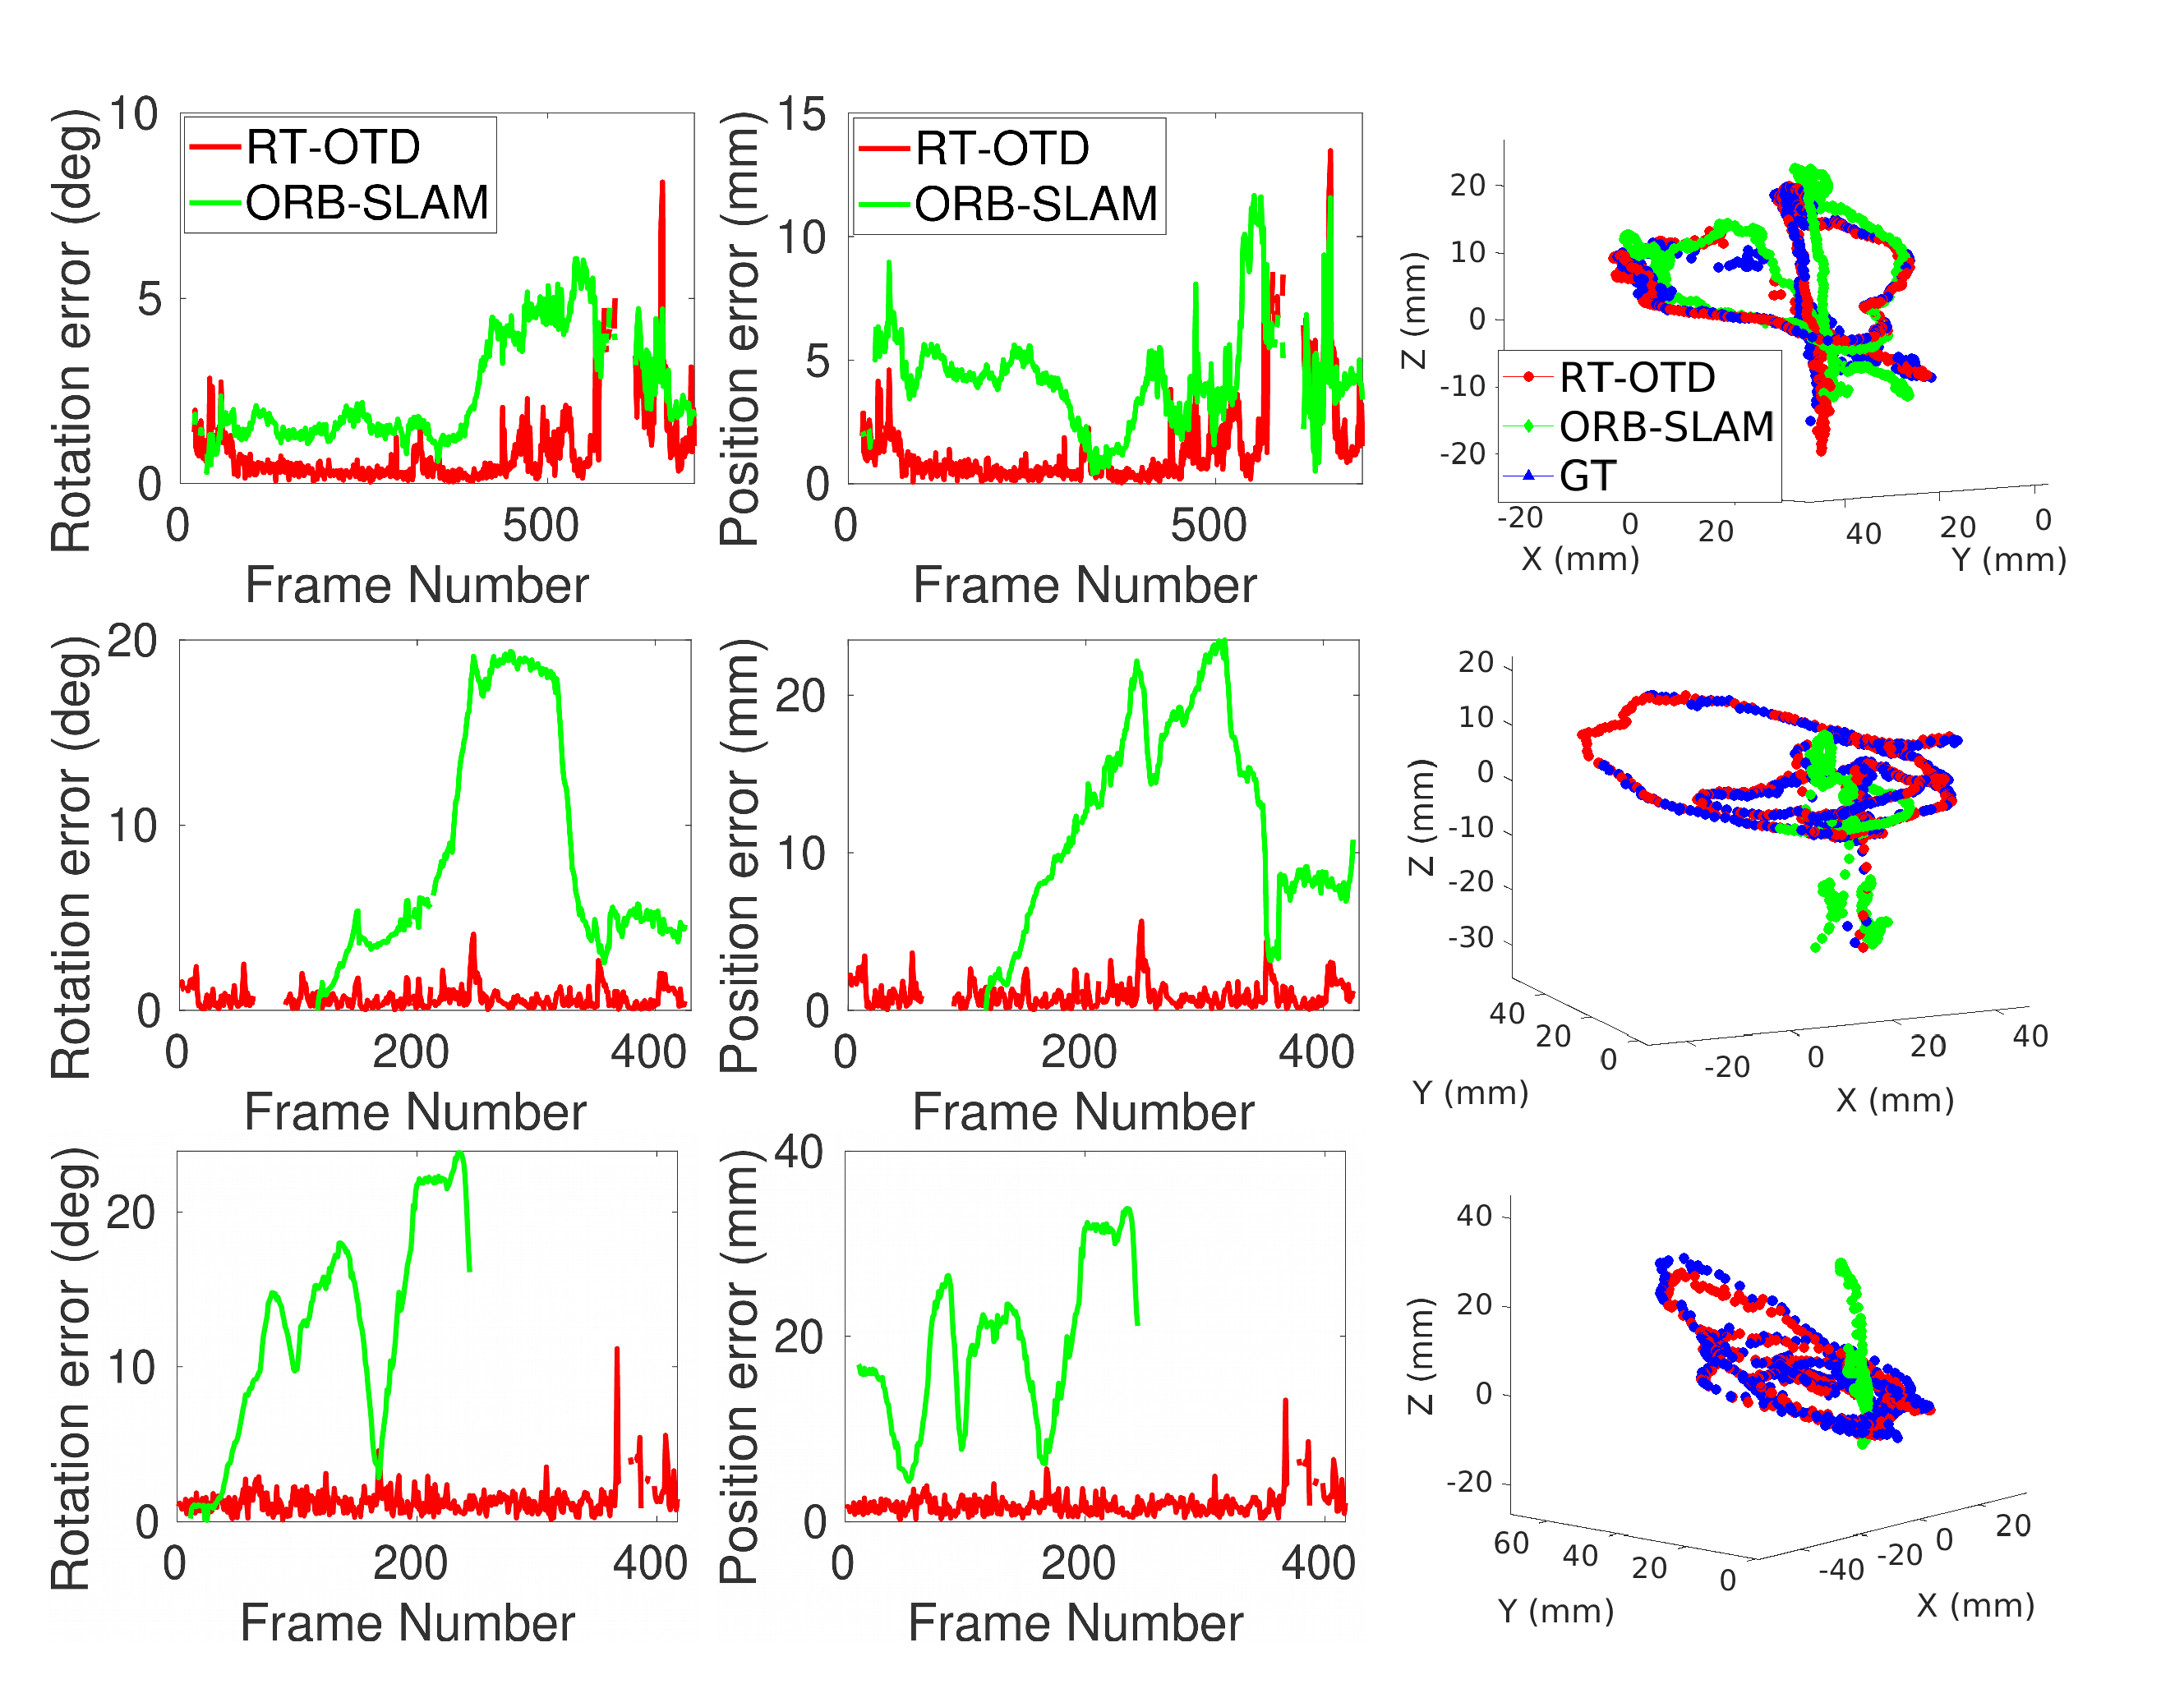
\includegraphics[width=0.78\columnwidth]{./figs/Accuracy_errors.pdf}
\caption{Rotation error, position error and camera trajectory, for $U_1$, $U_2$ and $U_3$ from top to bottom.}
\label{fig:hister_results}
 \vspace{-3mm}
\end{figure}
\SGG{In~\fig{fig:hister_results} we summarize the results of RT-OTD using \SG{SIFT} features.}
%We summarize the results of RT-OTD, using \SG{SIFT} features, against ORB-SLAM in \fig{fig:hister_results} for the three uteri.
The rotation error (in degrees) and position error (in mm) are computed as the Euclidean norm between GT and estimates.
There are gaps in the graphs when GT is not available.
\SGG{The results with RT-OTD are very accurate  and stable in all cases, with an average position error of $\SI{2}{\milli\metre}$  and an average rotation error of $\ang{3}$.}
%We also show the camera 3D trajectories estimated by RT-OTD and ORB-SLAM.
\SGG{\fig{fig:hister_results} also shows the tracking performed with a state-of-the-art open-source implementation of SLAM, ORB-SLAM.}
While it tracks a large portion of the first sequence, it quickly degenerates and loses the track for the other two cases.
This is due to the fact that SLAM builds a model with points from both the moving uterus and the background, violating the rigidity assumption.
It is also affected by motion blur and the lack of matches with the map.
%The results with RT-OTD are very accurate  and stable in all cases, with an average position error of $\SI{2}{\milli\metre}$  and an average rotation error of $\ang{3}$.


\subsubsection{Robustness Test for Tracking}
\label{subsec:robustTracking}
\SG{Since it is hard to obtain GT data in the laparoscopic setting, we evaluated tracking robustness \wrt occlusions from the keyframes used for 3D reconstruction, for which a reference pose is available from SfM, forming the GT. 
Using the data collected from $5$ patients, we simulated occlusions and compared the pose computed by the tracker to the GT. 
In a first experiment, we used the known mask of the uterus to add a black occluder starting from the external contour and towards the center of the uterus.
We gradually increased the size of the occluder and launched tracking on the keyframe.
\fig{fig:statsKframeSelection}.e shows the overall percentage of frames that could be tracked against the occlusion ratio.
The occlusion ratio is computed from the number of pixels of the occluder and of the uterus.
The graph shows that tracking copes with up to $\SI{60}{\percent}$ occlusion, where $\sim\SI{80}{\percent}$ of the frames are tracked.
For the same experiment, \fig{fig:statsKframeSelection}.f shows that the pose rotational error is below $\sim\ang{1}$ for up to $\SI{50}{\percent}$ occlusion.}
\SG{In a second experiment we simulated the presence of tools or bleeding covering the appearance of the uterus by growing black spots randomly distributed on the the uterus.
\fig{fig:statsKframeSelection}.g shows that tracking successfully estimates pose for up to $\SI{60}{\percent}$ occlusion, where $\sim\SI{90}{\percent}$ of the frames are tracked, with rotational error below or of the order of $\sim\ang{1}$.}
\SGG{We refer the reader to \url{https://bit.ly/2WKO6hI}) for quantitative and qualitative evaluation of the robustness.}

\begin{figure}
  \centering
  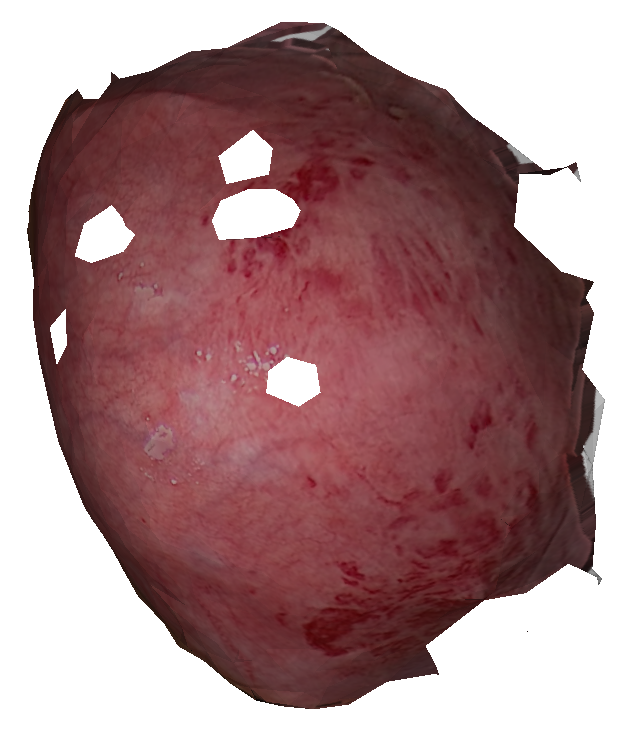
\includegraphics[width=0.12\columnwidth]{./figs/kframeSelection/beginning.png}\hspace{0.5mm}
  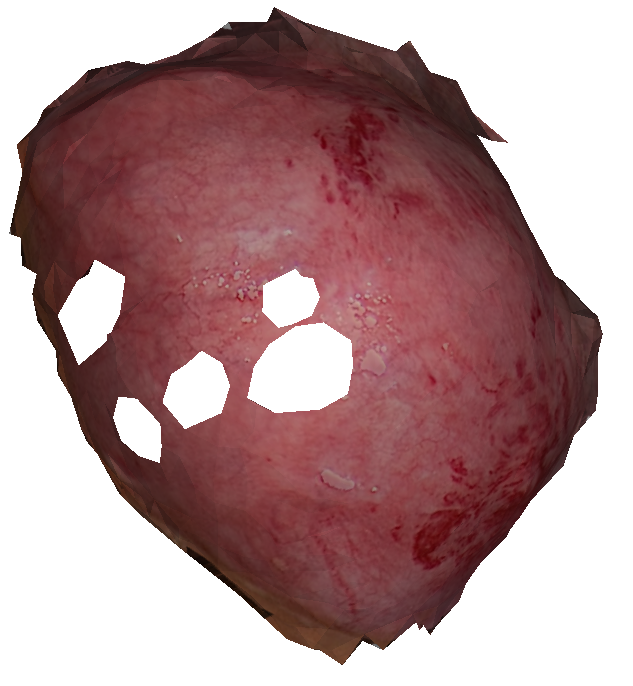
\includegraphics[width=0.12\columnwidth]{./figs/kframeSelection/middle.png}\hspace{0.5mm}
  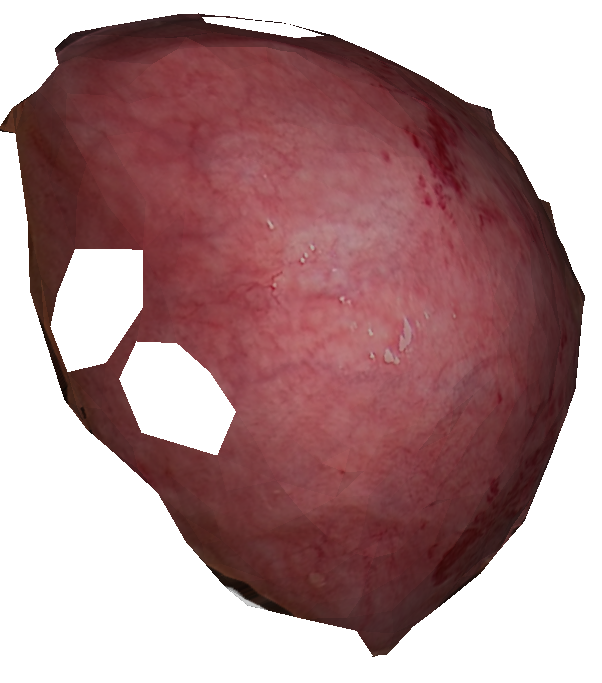
\includegraphics[width=0.12\columnwidth]{./figs/kframeSelection/end.png}\hspace{0.5mm}
  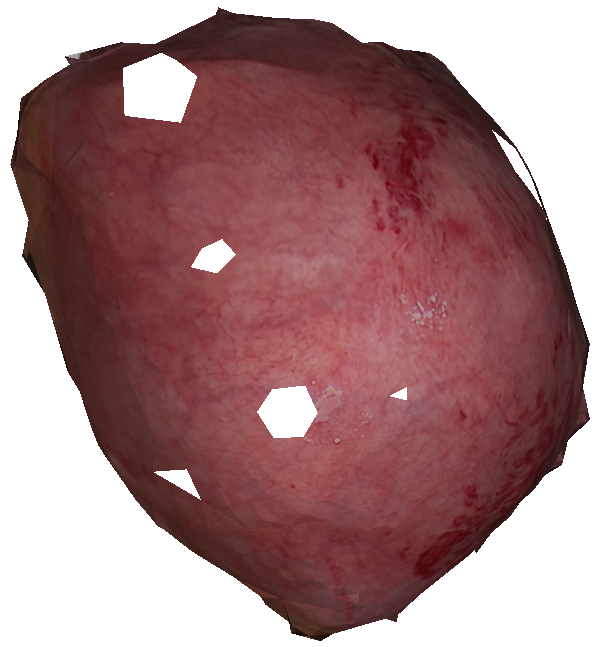
\includegraphics[width=0.12\columnwidth]{./figs/kframeSelection/equally.png}\hspace{0.5mm}
  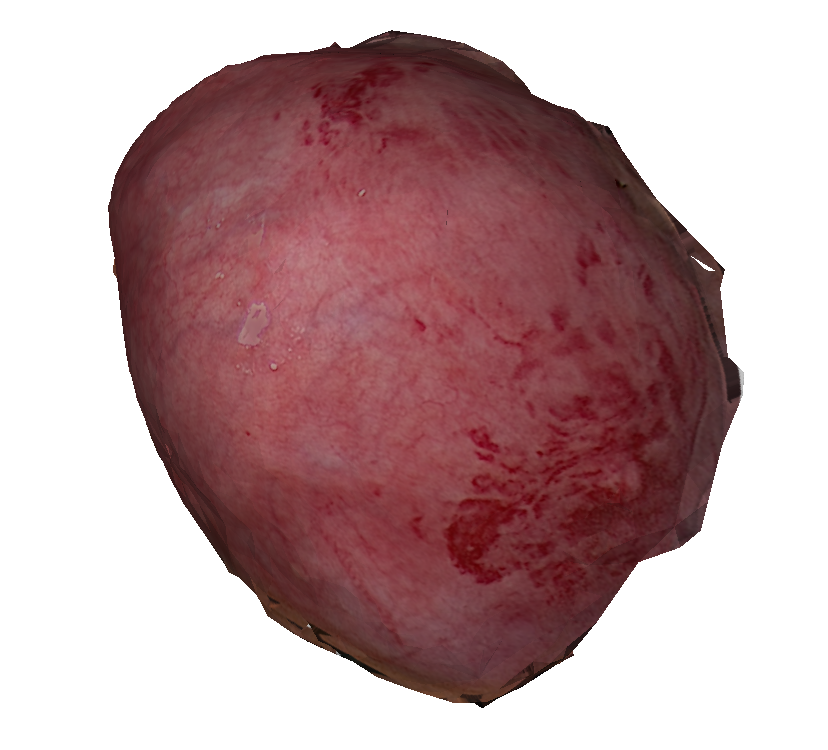
\includegraphics[width=0.15\columnwidth]{./figs/kframeSelection/auto.png}
  \caption{From left to right, the 3D models generated using the keyframes extracted with \emph{beginning}, \emph{middle}, \emph{end}, \emph{equally}, \emph{auto}.}
  \label{fig:3DresultsKframeSelection}
\end{figure}

\begin{figure*}[htbp]
\centering
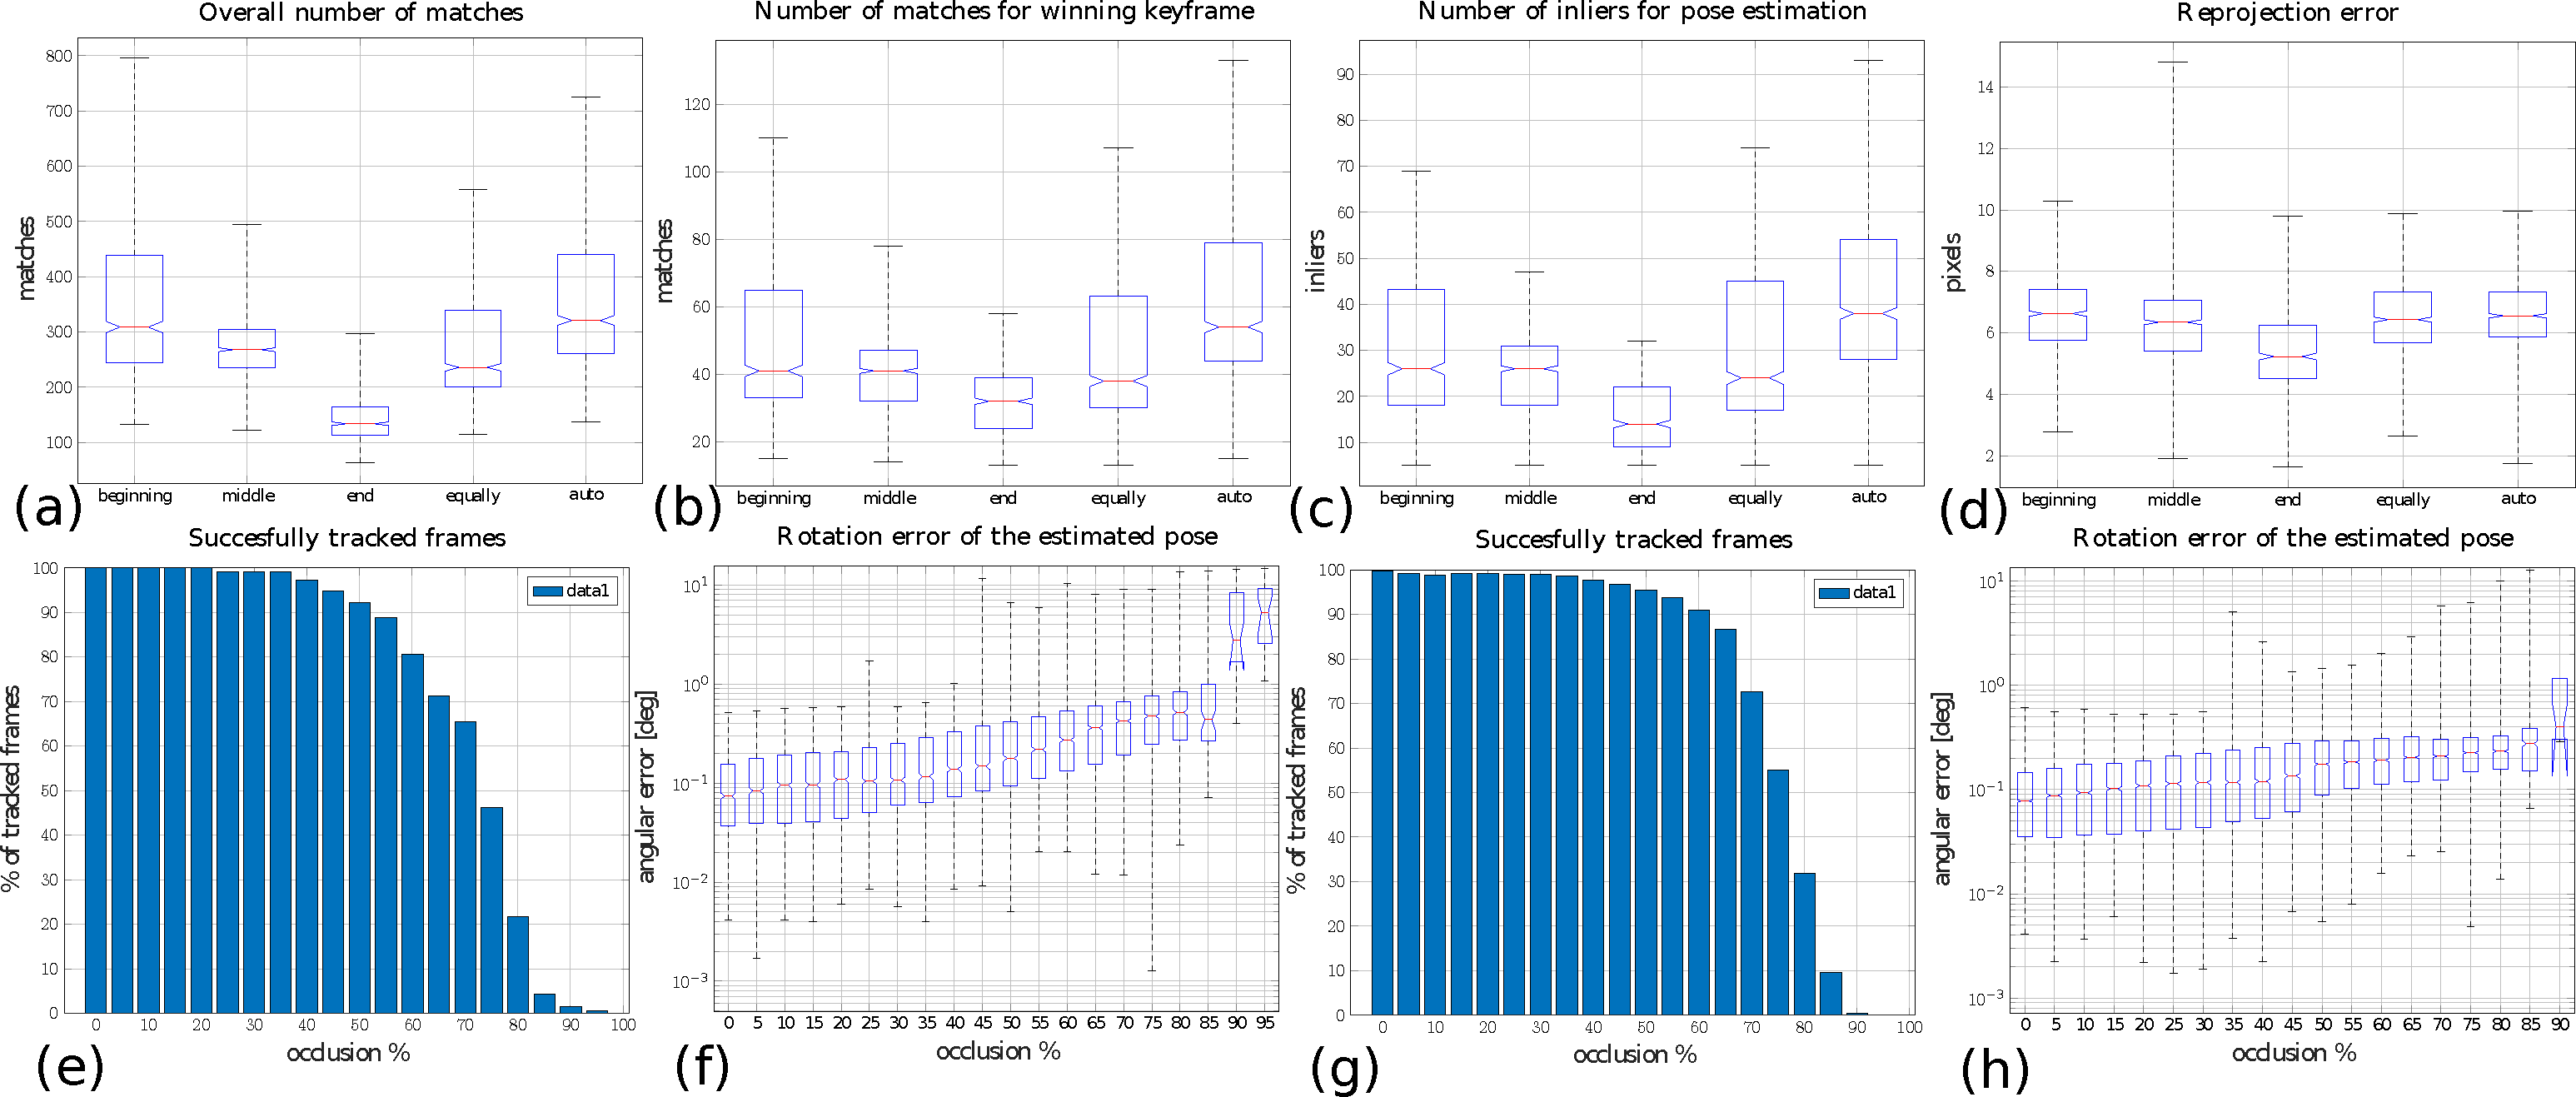
\includegraphics[width=0.8\textwidth]{./figs/ResultsC.pdf}
\caption{(a,b,c,d) Tracking statistics (number of matches, inliers, and pose errors) for each keyframe sampling method.% ( In each graph, the box plot represents the statistical distribution of the data, the blue box represents the second and third quartiles with a notch on the median value, while the whiskers represents the max and min values. 
(e,f,g,h) From left to right, histogram of successfully tracked frames and rotation error of estimated pose, for both experiments.}
\label{fig:statsKframeSelection}
\end{figure*}

%\begin{figure}
%  \centering
%  \begin{tabular}{cc}
%  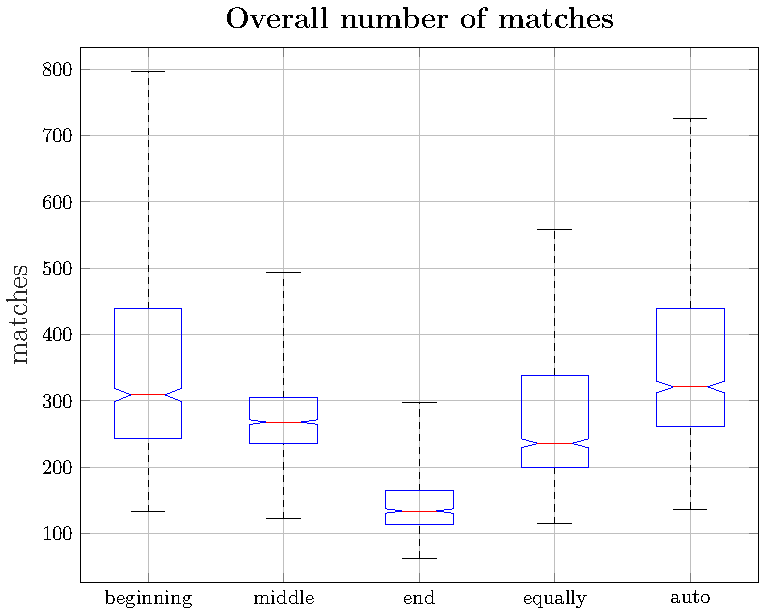
\includegraphics[width=0.20\textwidth]{./figs/kframeSelection/matching.pdf}&
% 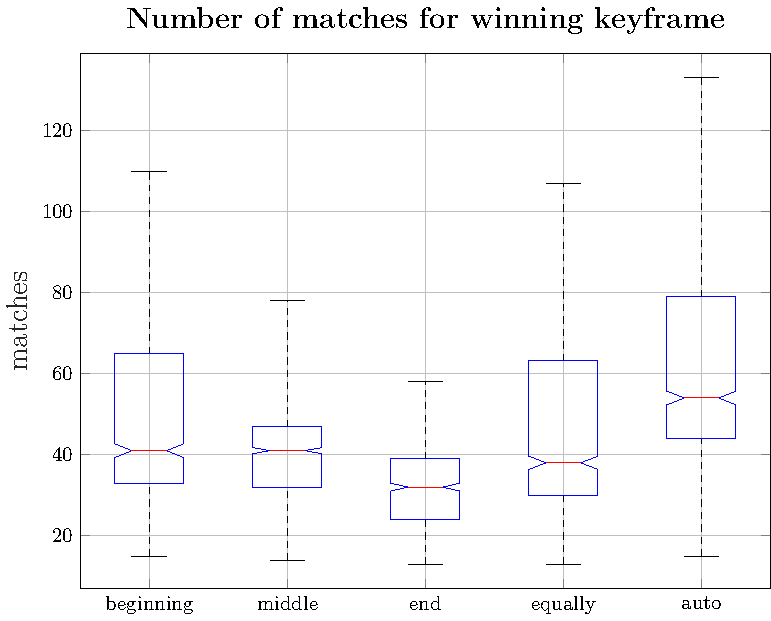
\includegraphics[width=0.20\textwidth]{./figs/kframeSelection/matcheswinningKF.pdf}\\
%  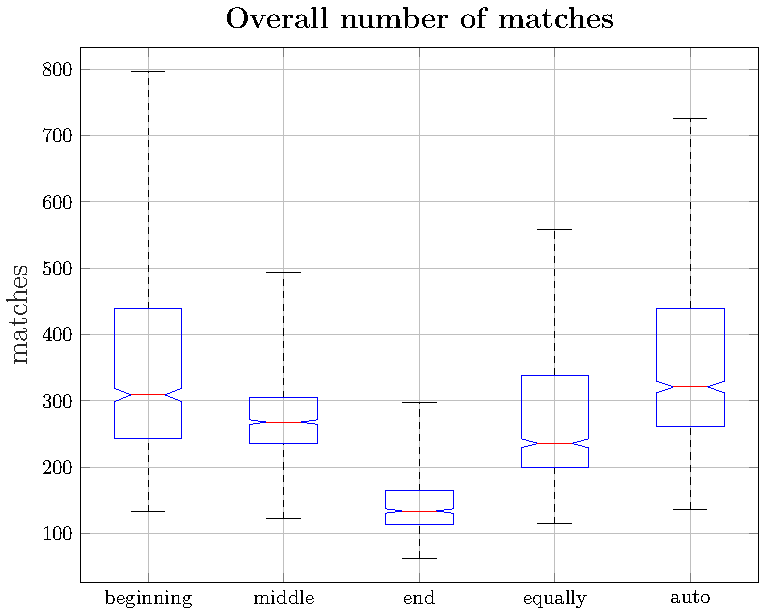
\includegraphics[width=0.20\textwidth]{./figs/kframeSelection/matching.pdf}&
%  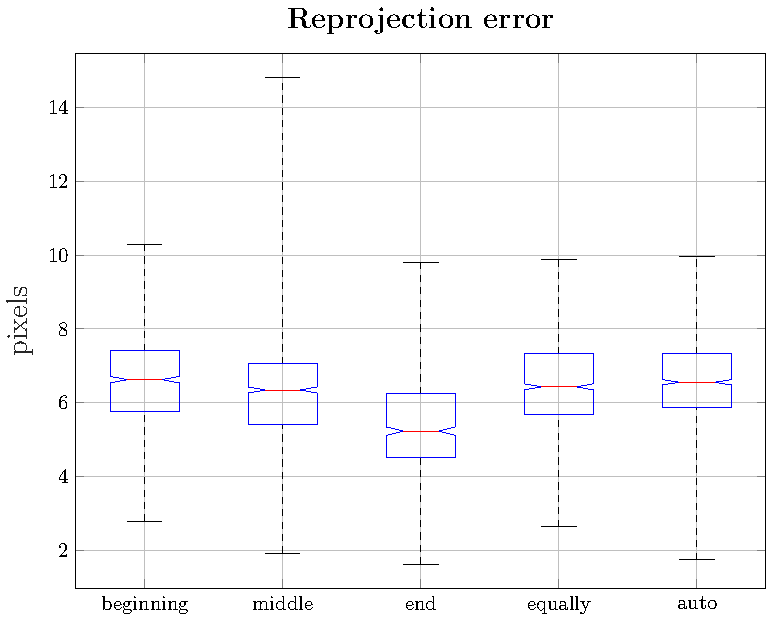
\includegraphics[width=0.20\textwidth]{./figs/kframeSelection/rmsePnP.pdf}
%  \end{tabular}
%\caption{In each graph, the box plot represents the statistical distribution of the data, the blue box represents the second and third quartiles with a notch on the median value, while the whiskers represents the max and min values.}
%\label{fig:statsKframeSelection}
%\end{figure}

%\begin{figure}
%  \centering
%%  \include{./figs/stresstest/histo_all}
%  \begin{tabular}{cc}
%  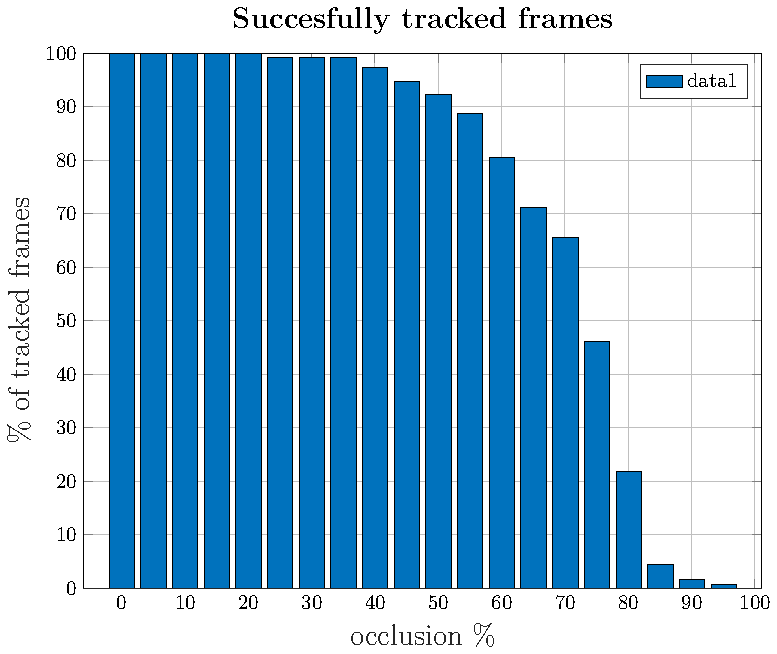
\includegraphics[width=0.20\textwidth]{./figs/stresstest/trackingHisto.pdf}&
% 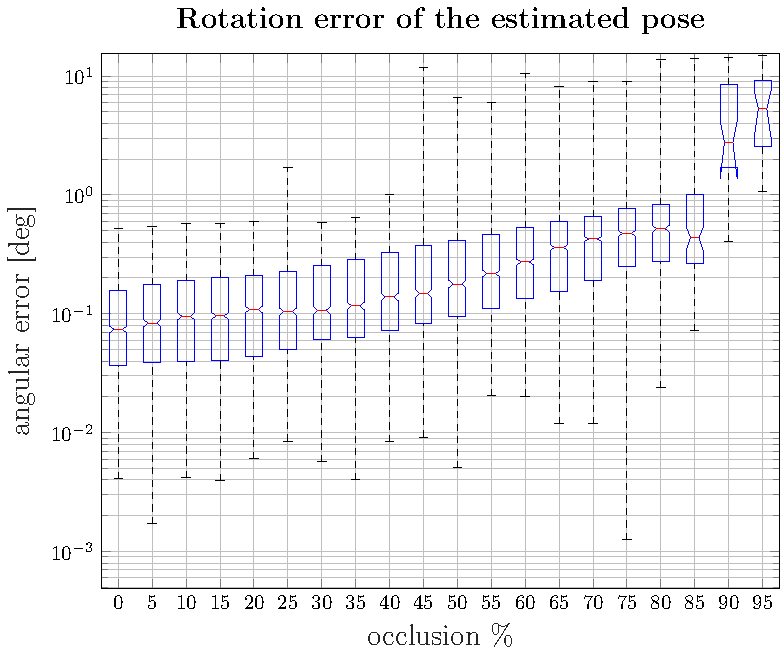
\includegraphics[width=0.20\textwidth]{./figs/stresstest/rotError.pdf}\\
%  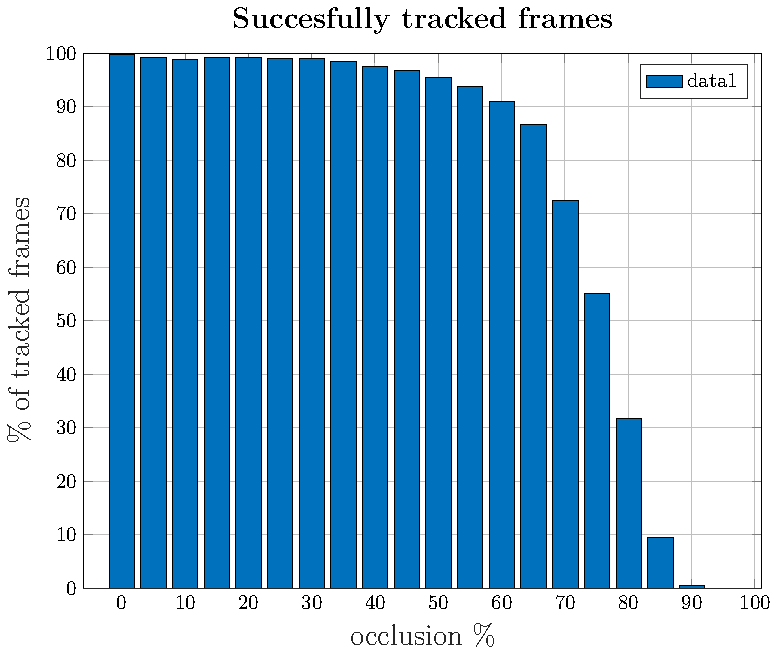
\includegraphics[width=0.20\textwidth]{./figs/stresstest/trackingHistoPois.pdf}&
% 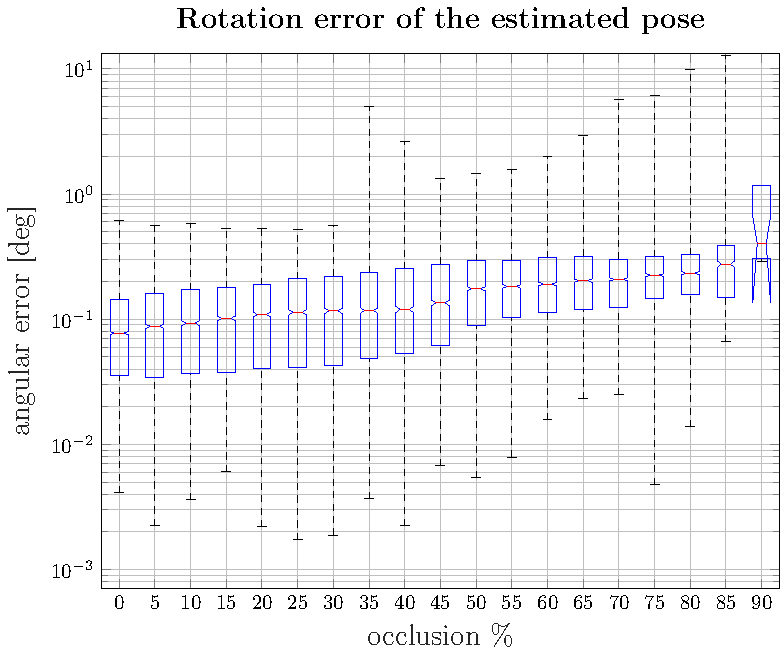
\includegraphics[width=0.20\textwidth]{./figs/stresstest/rotErrorPois.pdf}
% \end{tabular}
%  \caption{From left to right, histogram of successfully tracked frames and rotation error of estimated pose, for both experiments.}
% \label{fig:stressTest}
%\end{figure}


\subsubsection{Additional Keyframes During Tracking}
\label{sec:exp_additionalkeyframes}
\SG{We present results to show the impact of adding keyframes during tracking.
We refer the reader to the video material to observe the qualitative impact on the stability of pose and quality of AR (\url{https://bit.ly/34wEhXu}).
\tab{tab:addKf} shows the number of tracked keyframes for three videos with and without additional frames.
Importantly, even a single new keyframe can greatly improve the number of tracked frames, as in video 20190801 in which it almost doubles the number of tracked frames.
In general however, the number of tracked frames does not vary considerably but the tracking is much more stable.}


\begin{table}[]
  \begin{tabular}{ll|l|ll}
    video id & \# frames & \begin{tabular}[c]{@{}l@{}}\% tracked w/o \\ additional keyframes\end{tabular} & \begin{tabular}[c]{@{}l@{}}added \\ keyframes\end{tabular} & \% tracked \\
    \hline
    \hline
    20190801 & $1943$      & $\SI{55.58}{\percent}$                             & $1$              & $\SI{99.90}{\percent}$     \\
    20190612 & $5119$      &  $\SI{95.64}{\percent}$                                   & $8$                & $\SI{97.15}{\percent}$     \\
    20190724 & $2444$          & $\SI{87.52}{\percent}$                                    & $4$               & $\SI{87.96}{\percent}$
  \end{tabular}
  \caption{Number of tracked frames with and without adding new keyframes during tracking.}
  \label{tab:addKf}
\end{table}



\subsubsection{Computational Times}
Our hardware is composed of a desktop PC running Linux Ubuntu with an Intel Core i$7$-$5960$X CPU running at \SI{3.00}{\giga\hertz} with \SI{16}{\giga\byte} of RAM and an NVIDIA GeForce GTX $980$ Ti graphics card.
On average, tracking takes \SI{16.35}{\milli\second} with a full HD $1920\times1080$ image.
SIFT takes \SI{11.1}{\milli\second}, descriptor matching between $\mathcal{F}$ and $\mathcal{G}$ takes \SI{3.21}{\milli\second}  and pose estimation takes \SI{0.18}{\milli\second}.

% \subsubsection{Comparison with ORB SLAM}
% \label{sec:orbslam}
% We have compared with ORB-SLAM2, which provides state-of-the-art results monocular SLAM results on laparoscopic videos \cite{orbslam_laparo}. As discussed in \sect{sec:sotaTracking} a scene that consists of independently moving structures such as the uterus will cause difficulty for current monocular SLAM methods, because they will amalgamates features from different structures into one map. This can be extremely problematic when there is slow relative motion between the structures. \fig{fig:orbAR} shows an example of this problem. On the left, the ORB features used for tracking are shown, covering the uterus (foreground) and surrounding peritoneum. When the uterus is then moved significantly \wrt the surroundings, the pose is computed wrongly, because background features have a strong influence on the estimated pose.


% % \begin{figure}
% % \centering
% % % This file was created by matlab2tikz.
%
%The latest updates can be retrieved from
%  http://www.mathworks.com/matlabcentral/fileexchange/22022-matlab2tikz-matlab2tikz
%where you can also make suggestions and rate matlab2tikz.
%
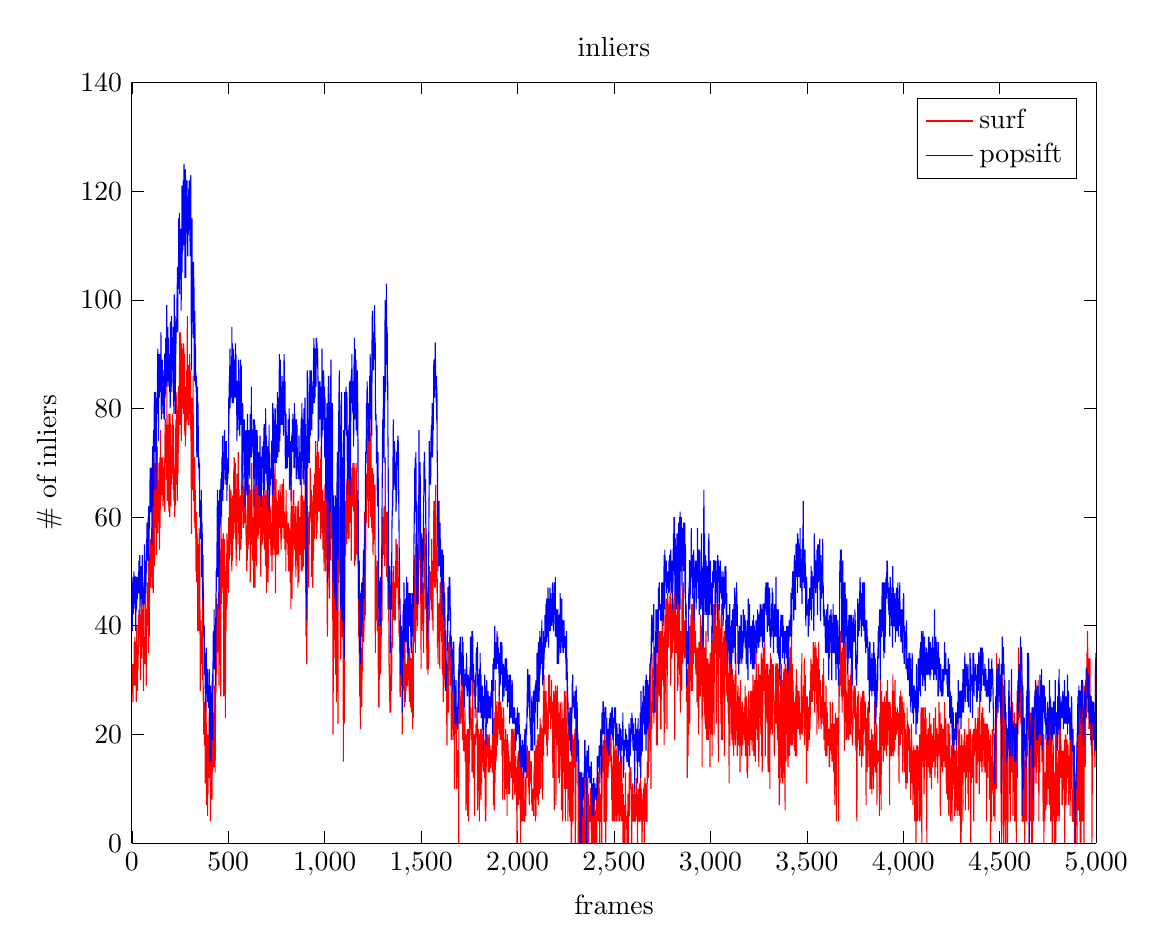
\begin{tikzpicture}

\begin{axis}[%
width=4.822in,
height=3.803in,
at={(0.809in,0.513in)},
scale only axis,
separate axis lines,
every outer x axis line/.append style={black},
every x tick label/.append style={font=\color{black}},
every x tick/.append style={black},
xmin=0,
xmax=5000,
xlabel={frames},
every outer y axis line/.append style={black},
every y tick label/.append style={font=\color{black}},
every y tick/.append style={black},
ymin=0,
ymax=140,
ylabel={\# of inliers},
axis background/.style={fill=white},
title={inliers},
legend style={legend cell align=left, align=left, draw=black}
]
\addplot [color=red, forget plot]
  table[row sep=crcr]{%
0	29\\
1	33\\
2	29\\
3	31\\
4	29\\
5	28\\
6	26\\
7	28\\
8	31\\
9	33\\
10	31\\
11	29\\
12	34\\
13	37\\
14	30\\
15	36\\
16	38\\
17	29\\
18	30\\
19	34\\
20	29\\
21	34\\
22	37\\
23	26\\
24	35\\
25	30\\
26	40\\
27	29\\
28	34\\
29	34\\
30	28\\
31	34\\
32	32\\
33	34\\
34	37\\
35	42\\
36	38\\
37	43\\
38	41\\
39	39\\
40	41\\
41	41\\
42	38\\
43	36\\
44	42\\
45	30\\
46	40\\
47	35\\
48	34\\
49	47\\
50	50\\
51	41\\
52	34\\
53	42\\
54	40\\
55	36\\
56	43\\
57	38\\
58	39\\
59	48\\
60	42\\
61	28\\
62	44\\
63	38\\
64	33\\
65	34\\
66	34\\
67	37\\
68	38\\
69	33\\
70	36\\
71	43\\
72	47\\
73	41\\
74	39\\
75	29\\
76	42\\
77	43\\
78	41\\
79	40\\
80	43\\
81	43\\
82	41\\
83	48\\
84	43\\
85	39\\
86	43\\
87	35\\
88	53\\
89	53\\
90	43\\
91	38\\
92	49\\
93	49\\
94	47\\
95	52\\
96	47\\
97	56\\
98	54\\
99	56\\
100	52\\
101	50\\
102	49\\
103	58\\
104	47\\
105	47\\
106	54\\
107	57\\
108	54\\
109	65\\
110	52\\
111	46\\
112	54\\
113	61\\
114	68\\
115	54\\
116	56\\
117	59\\
118	51\\
119	69\\
120	70\\
121	58\\
122	64\\
123	63\\
124	58\\
125	59\\
126	70\\
127	60\\
128	53\\
129	72\\
130	63\\
131	72\\
132	73\\
133	66\\
134	70\\
135	57\\
136	65\\
137	66\\
138	59\\
139	64\\
140	64\\
141	65\\
142	70\\
143	69\\
144	54\\
145	64\\
146	71\\
147	58\\
148	69\\
149	76\\
150	67\\
151	63\\
152	71\\
153	66\\
154	67\\
155	66\\
156	70\\
157	64\\
158	67\\
159	71\\
160	68\\
161	68\\
162	62\\
163	69\\
164	66\\
165	69\\
166	63\\
167	65\\
168	67\\
169	71\\
170	70\\
171	61\\
172	73\\
173	78\\
174	78\\
175	70\\
176	77\\
177	75\\
178	73\\
179	71\\
180	67\\
181	67\\
182	84\\
183	66\\
184	63\\
185	69\\
186	68\\
187	67\\
188	69\\
189	76\\
190	77\\
191	75\\
192	61\\
193	79\\
194	74\\
195	78\\
196	70\\
197	60\\
198	65\\
199	79\\
200	67\\
201	73\\
202	62\\
203	68\\
204	67\\
205	66\\
206	73\\
207	68\\
208	77\\
209	74\\
210	68\\
211	71\\
212	79\\
213	70\\
214	67\\
215	65\\
216	77\\
217	75\\
218	67\\
219	63\\
220	63\\
221	69\\
222	66\\
223	60\\
224	69\\
225	62\\
226	66\\
227	70\\
228	76\\
229	78\\
230	69\\
231	69\\
232	66\\
233	82\\
234	83\\
235	65\\
236	63\\
237	69\\
238	77\\
239	78\\
240	68\\
241	74\\
242	76\\
243	84\\
244	75\\
245	84\\
246	84\\
247	77\\
248	94\\
249	77\\
250	80\\
251	89\\
252	88\\
253	94\\
254	82\\
255	82\\
256	79\\
257	74\\
258	82\\
259	92\\
260	89\\
261	83\\
262	89\\
263	80\\
264	81\\
265	83\\
266	91\\
267	90\\
268	79\\
269	92\\
270	85\\
271	84\\
272	90\\
273	89\\
274	82\\
275	75\\
276	76\\
277	78\\
278	73\\
279	84\\
280	75\\
281	79\\
282	77\\
283	83\\
284	80\\
285	87\\
286	80\\
287	84\\
288	97\\
289	78\\
290	82\\
291	78\\
292	83\\
293	77\\
294	77\\
295	88\\
296	79\\
297	83\\
298	79\\
299	79\\
300	90\\
301	84\\
302	80\\
303	77\\
304	87\\
305	86\\
306	76\\
307	74\\
308	77\\
309	57\\
310	57\\
311	81\\
312	82\\
313	72\\
314	65\\
315	75\\
316	79\\
317	71\\
318	86\\
319	68\\
320	74\\
321	63\\
322	65\\
323	71\\
324	70\\
325	59\\
326	67\\
327	71\\
328	58\\
329	65\\
330	59\\
331	57\\
332	56\\
333	50\\
334	61\\
335	48\\
336	53\\
337	48\\
338	52\\
339	57\\
340	51\\
341	53\\
342	39\\
343	53\\
344	55\\
345	44\\
346	44\\
347	51\\
348	39\\
349	58\\
350	43\\
351	57\\
352	56\\
353	46\\
354	38\\
355	28\\
356	41\\
357	36\\
358	37\\
359	41\\
360	34\\
361	38\\
362	33\\
363	37\\
364	39\\
365	37\\
366	39\\
367	30\\
368	44\\
369	48\\
370	27\\
371	26\\
372	29\\
373	20\\
374	22\\
375	25\\
376	26\\
377	18\\
378	22\\
379	18\\
380	24\\
381	11\\
382	20\\
383	12\\
384	13\\
385	26\\
386	21\\
387	12\\
388	7\\
389	18\\
390	20\\
391	15\\
392	20\\
393	5\\
394	20\\
395	9\\
396	19\\
397	15\\
398	17\\
399	12\\
400	16\\
401	17\\
402	24\\
403	20\\
404	20\\
405	16\\
406	21\\
407	11\\
408	4\\
409	17\\
410	16\\
411	12\\
412	17\\
413	22\\
414	22\\
415	13\\
416	8\\
417	25\\
418	22\\
419	13\\
420	14\\
421	20\\
422	24\\
423	18\\
424	20\\
425	21\\
426	16\\
427	14\\
428	23\\
429	29\\
430	24\\
431	19\\
432	13\\
433	18\\
434	23\\
435	31\\
436	28\\
437	28\\
438	33\\
439	45\\
440	31\\
441	33\\
442	39\\
443	42\\
444	35\\
445	38\\
446	44\\
447	43\\
448	41\\
449	46\\
450	46\\
451	42\\
452	29\\
453	30\\
454	45\\
455	54\\
456	46\\
457	42\\
458	48\\
459	43\\
460	35\\
461	27\\
462	66\\
463	46\\
464	44\\
465	55\\
466	49\\
467	49\\
468	56\\
469	47\\
470	53\\
471	56\\
472	52\\
473	46\\
474	57\\
475	49\\
476	39\\
477	27\\
478	53\\
479	56\\
480	55\\
481	49\\
482	48\\
483	46\\
484	51\\
485	23\\
486	34\\
487	45\\
488	47\\
489	39\\
490	50\\
491	43\\
492	47\\
493	57\\
494	44\\
495	53\\
496	49\\
497	47\\
498	48\\
499	54\\
500	55\\
501	57\\
502	46\\
503	60\\
504	55\\
505	52\\
506	60\\
507	66\\
508	53\\
509	60\\
510	53\\
511	65\\
512	59\\
513	55\\
514	65\\
515	61\\
516	58\\
517	61\\
518	52\\
519	50\\
520	61\\
521	52\\
522	63\\
523	64\\
524	55\\
525	60\\
526	56\\
527	57\\
528	62\\
529	69\\
530	57\\
531	71\\
532	62\\
533	68\\
534	62\\
535	60\\
536	64\\
537	70\\
538	59\\
539	56\\
540	58\\
541	51\\
542	55\\
543	64\\
544	59\\
545	68\\
546	64\\
547	66\\
548	67\\
549	68\\
550	55\\
551	60\\
552	72\\
553	62\\
554	59\\
555	65\\
556	65\\
557	59\\
558	60\\
559	52\\
560	60\\
561	61\\
562	55\\
563	61\\
564	64\\
565	54\\
566	60\\
567	62\\
568	56\\
569	66\\
570	61\\
571	66\\
572	71\\
573	61\\
574	63\\
575	65\\
576	63\\
577	58\\
578	63\\
579	62\\
580	58\\
581	68\\
582	62\\
583	60\\
584	61\\
585	59\\
586	60\\
587	59\\
588	59\\
589	66\\
590	62\\
591	61\\
592	58\\
593	55\\
594	55\\
595	56\\
596	50\\
597	58\\
598	54\\
599	52\\
600	59\\
601	66\\
602	62\\
603	54\\
604	62\\
605	55\\
606	60\\
607	66\\
608	56\\
609	63\\
610	62\\
611	66\\
612	60\\
613	63\\
614	48\\
615	61\\
616	64\\
617	62\\
618	65\\
619	55\\
620	64\\
621	57\\
622	70\\
623	65\\
624	56\\
625	52\\
626	60\\
627	56\\
628	56\\
629	58\\
630	58\\
631	50\\
632	47\\
633	59\\
634	66\\
635	57\\
636	60\\
637	48\\
638	63\\
639	47\\
640	65\\
641	54\\
642	59\\
643	70\\
644	57\\
645	52\\
646	58\\
647	51\\
648	60\\
649	69\\
650	68\\
651	66\\
652	68\\
653	61\\
654	63\\
655	56\\
656	58\\
657	64\\
658	58\\
659	60\\
660	59\\
661	61\\
662	66\\
663	62\\
664	58\\
665	65\\
666	58\\
667	54\\
668	54\\
669	49\\
670	56\\
671	57\\
672	64\\
673	55\\
674	55\\
675	63\\
676	55\\
677	58\\
678	60\\
679	64\\
680	58\\
681	64\\
682	59\\
683	57\\
684	59\\
685	56\\
686	70\\
687	56\\
688	54\\
689	57\\
690	61\\
691	64\\
692	59\\
693	51\\
694	53\\
695	59\\
696	65\\
697	59\\
698	46\\
699	62\\
700	57\\
701	56\\
702	48\\
703	56\\
704	65\\
705	64\\
706	48\\
707	49\\
708	56\\
709	59\\
710	61\\
711	60\\
712	56\\
713	63\\
714	64\\
715	60\\
716	56\\
717	62\\
718	61\\
719	55\\
720	57\\
721	54\\
722	53\\
723	53\\
724	55\\
725	59\\
726	57\\
727	50\\
728	62\\
729	59\\
730	70\\
731	53\\
732	55\\
733	57\\
734	62\\
735	69\\
736	63\\
737	59\\
738	58\\
739	54\\
740	66\\
741	62\\
742	53\\
743	72\\
744	57\\
745	46\\
746	57\\
747	62\\
748	67\\
749	62\\
750	57\\
751	53\\
752	54\\
753	61\\
754	63\\
755	56\\
756	61\\
757	58\\
758	63\\
759	53\\
760	56\\
761	65\\
762	59\\
763	61\\
764	61\\
765	63\\
766	58\\
767	61\\
768	59\\
769	66\\
770	63\\
771	64\\
772	57\\
773	63\\
774	54\\
775	57\\
776	57\\
777	56\\
778	57\\
779	66\\
780	66\\
781	60\\
782	64\\
783	64\\
784	58\\
785	61\\
786	66\\
787	67\\
788	63\\
789	56\\
790	59\\
791	61\\
792	60\\
793	59\\
794	54\\
795	60\\
796	59\\
797	55\\
798	59\\
799	50\\
800	65\\
801	58\\
802	61\\
803	57\\
804	61\\
805	56\\
806	56\\
807	56\\
808	55\\
809	57\\
810	53\\
811	54\\
812	59\\
813	53\\
814	50\\
815	56\\
816	55\\
817	58\\
818	57\\
819	56\\
820	55\\
821	48\\
822	54\\
823	53\\
824	55\\
825	43\\
826	67\\
827	56\\
828	62\\
829	57\\
830	54\\
831	45\\
832	62\\
833	60\\
834	50\\
835	53\\
836	53\\
837	65\\
838	60\\
839	55\\
840	65\\
841	56\\
842	60\\
843	56\\
844	58\\
845	54\\
846	55\\
847	56\\
848	62\\
849	51\\
850	54\\
851	49\\
852	62\\
853	53\\
854	58\\
855	53\\
856	59\\
857	52\\
858	55\\
859	53\\
860	62\\
861	47\\
862	53\\
863	63\\
864	61\\
865	55\\
866	48\\
867	51\\
868	55\\
869	58\\
870	55\\
871	59\\
872	60\\
873	54\\
874	57\\
875	53\\
876	58\\
877	64\\
878	55\\
879	50\\
880	69\\
881	57\\
882	57\\
883	50\\
884	51\\
885	61\\
886	64\\
887	57\\
888	51\\
889	51\\
890	59\\
891	51\\
892	63\\
893	57\\
894	55\\
895	54\\
896	56\\
897	61\\
898	61\\
899	69\\
900	56\\
901	68\\
902	53\\
903	38\\
904	46\\
905	57\\
906	56\\
907	33\\
908	37\\
909	59\\
910	62\\
911	59\\
912	56\\
913	60\\
914	56\\
915	53\\
916	54\\
917	47\\
918	57\\
919	61\\
920	55\\
921	59\\
922	60\\
923	60\\
924	60\\
925	69\\
926	67\\
927	64\\
928	64\\
929	63\\
930	59\\
931	65\\
932	49\\
933	57\\
934	57\\
935	64\\
936	61\\
937	51\\
938	47\\
939	59\\
940	55\\
941	52\\
942	54\\
943	66\\
944	65\\
945	64\\
946	60\\
947	56\\
948	68\\
949	58\\
950	62\\
951	61\\
952	65\\
953	74\\
954	70\\
955	62\\
956	69\\
957	56\\
958	68\\
959	63\\
960	65\\
961	57\\
962	74\\
963	59\\
964	72\\
965	63\\
966	65\\
967	61\\
968	72\\
969	62\\
970	68\\
971	68\\
972	62\\
973	63\\
974	61\\
975	69\\
976	66\\
977	64\\
978	62\\
979	56\\
980	71\\
981	62\\
982	73\\
983	63\\
984	59\\
985	58\\
986	60\\
987	57\\
988	61\\
989	58\\
990	65\\
991	54\\
992	62\\
993	62\\
994	63\\
995	62\\
996	59\\
997	50\\
998	53\\
999	61\\
1000	52\\
1001	57\\
1002	66\\
1003	61\\
1004	60\\
1005	50\\
1006	57\\
1007	61\\
1008	63\\
1009	59\\
1010	56\\
1011	59\\
1012	57\\
1013	45\\
1014	38\\
1015	41\\
1016	52\\
1017	59\\
1018	64\\
1019	60\\
1020	65\\
1021	60\\
1022	68\\
1023	63\\
1024	47\\
1025	45\\
1026	53\\
1027	63\\
1028	66\\
1029	72\\
1030	52\\
1031	56\\
1032	57\\
1033	67\\
1034	57\\
1035	61\\
1036	56\\
1037	77\\
1038	76\\
1039	70\\
1040	49\\
1041	61\\
1042	46\\
1043	20\\
1044	22\\
1045	47\\
1046	48\\
1047	55\\
1048	52\\
1049	34\\
1050	42\\
1051	40\\
1052	43\\
1053	39\\
1054	53\\
1055	48\\
1056	49\\
1057	31\\
1058	51\\
1059	42\\
1060	36\\
1061	26\\
1062	48\\
1063	60\\
1064	44\\
1065	54\\
1066	67\\
1067	45\\
1068	36\\
1069	22\\
1070	49\\
1071	48\\
1072	48\\
1073	50\\
1074	69\\
1075	65\\
1076	56\\
1077	60\\
1078	52\\
1079	53\\
1080	58\\
1081	44\\
1082	41\\
1083	34\\
1084	34\\
1085	49\\
1086	52\\
1087	61\\
1088	68\\
1089	62\\
1090	48\\
1091	38\\
1092	38\\
1093	65\\
1094	55\\
1095	46\\
1096	36\\
1097	15\\
1098	57\\
1099	63\\
1100	65\\
1101	36\\
1102	22\\
1103	32\\
1104	49\\
1105	60\\
1106	62\\
1107	53\\
1108	53\\
1109	63\\
1110	60\\
1111	60\\
1112	56\\
1113	55\\
1114	66\\
1115	64\\
1116	67\\
1117	60\\
1118	69\\
1119	57\\
1120	70\\
1121	64\\
1122	56\\
1123	61\\
1124	72\\
1125	66\\
1126	56\\
1127	66\\
1128	63\\
1129	69\\
1130	59\\
1131	62\\
1132	70\\
1133	60\\
1134	61\\
1135	64\\
1136	67\\
1137	61\\
1138	52\\
1139	66\\
1140	64\\
1141	69\\
1142	69\\
1143	62\\
1144	64\\
1145	67\\
1146	66\\
1147	70\\
1148	64\\
1149	63\\
1150	61\\
1151	65\\
1152	62\\
1153	70\\
1154	61\\
1155	51\\
1156	62\\
1157	64\\
1158	64\\
1159	64\\
1160	52\\
1161	56\\
1162	64\\
1163	70\\
1164	68\\
1165	65\\
1166	62\\
1167	56\\
1168	53\\
1169	65\\
1170	61\\
1171	62\\
1172	60\\
1173	52\\
1174	45\\
1175	52\\
1176	38\\
1177	49\\
1178	39\\
1179	38\\
1180	33\\
1181	30\\
1182	27\\
1183	33\\
1184	32\\
1185	21\\
1186	35\\
1187	26\\
1188	25\\
1189	30\\
1190	31\\
1191	36\\
1192	25\\
1193	33\\
1194	30\\
1195	33\\
1196	39\\
1197	38\\
1198	49\\
1199	41\\
1200	43\\
1201	37\\
1202	42\\
1203	37\\
1204	40\\
1205	49\\
1206	61\\
1207	46\\
1208	41\\
1209	52\\
1210	51\\
1211	42\\
1212	60\\
1213	54\\
1214	60\\
1215	60\\
1216	66\\
1217	59\\
1218	68\\
1219	63\\
1220	65\\
1221	67\\
1222	70\\
1223	68\\
1224	81\\
1225	71\\
1226	71\\
1227	67\\
1228	58\\
1229	68\\
1230	72\\
1231	81\\
1232	78\\
1233	63\\
1234	68\\
1235	72\\
1236	71\\
1237	71\\
1238	66\\
1239	60\\
1240	79\\
1241	64\\
1242	62\\
1243	61\\
1244	58\\
1245	62\\
1246	65\\
1247	57\\
1248	69\\
1249	63\\
1250	57\\
1251	53\\
1252	64\\
1253	68\\
1254	55\\
1255	59\\
1256	56\\
1257	56\\
1258	57\\
1259	57\\
1260	58\\
1261	66\\
1262	43\\
1263	35\\
1264	50\\
1265	53\\
1266	46\\
1267	52\\
1268	46\\
1269	48\\
1270	41\\
1271	51\\
1272	42\\
1273	42\\
1274	39\\
1275	52\\
1276	42\\
1277	42\\
1278	32\\
1279	35\\
1280	25\\
1281	26\\
1282	25\\
1283	32\\
1284	41\\
1285	34\\
1286	42\\
1287	33\\
1288	39\\
1289	44\\
1290	31\\
1291	37\\
1292	36\\
1293	38\\
1294	41\\
1295	48\\
1296	41\\
1297	41\\
1298	51\\
1299	56\\
1300	60\\
1301	53\\
1302	59\\
1303	53\\
1304	55\\
1305	54\\
1306	57\\
1307	58\\
1308	62\\
1309	57\\
1310	55\\
1311	51\\
1312	57\\
1313	58\\
1314	71\\
1315	60\\
1316	55\\
1317	59\\
1318	55\\
1319	57\\
1320	61\\
1321	49\\
1322	60\\
1323	55\\
1324	54\\
1325	55\\
1326	61\\
1327	51\\
1328	43\\
1329	50\\
1330	55\\
1331	47\\
1332	41\\
1333	41\\
1334	31\\
1335	33\\
1336	30\\
1337	26\\
1338	31\\
1339	24\\
1340	31\\
1341	28\\
1342	27\\
1343	24\\
1344	37\\
1345	36\\
1346	28\\
1347	29\\
1348	33\\
1349	38\\
1350	38\\
1351	36\\
1352	48\\
1353	45\\
1354	50\\
1355	47\\
1356	47\\
1357	51\\
1358	46\\
1359	43\\
1360	41\\
1361	44\\
1362	41\\
1363	42\\
1364	48\\
1365	46\\
1366	41\\
1367	52\\
1368	51\\
1369	45\\
1370	56\\
1371	53\\
1372	49\\
1373	49\\
1374	50\\
1375	48\\
1376	47\\
1377	55\\
1378	48\\
1379	48\\
1380	52\\
1381	48\\
1382	43\\
1383	49\\
1384	49\\
1385	40\\
1386	38\\
1387	38\\
1388	41\\
1389	39\\
1390	32\\
1391	27\\
1392	27\\
1393	30\\
1394	36\\
1395	31\\
1396	29\\
1397	30\\
1398	33\\
1399	34\\
1400	34\\
1401	34\\
1402	20\\
1403	30\\
1404	33\\
1405	32\\
1406	31\\
1407	42\\
1408	28\\
1409	38\\
1410	42\\
1411	32\\
1412	36\\
1413	25\\
1414	39\\
1415	34\\
1416	39\\
1417	35\\
1418	26\\
1419	31\\
1420	33\\
1421	31\\
1422	28\\
1423	31\\
1424	30\\
1425	33\\
1426	31\\
1427	31\\
1428	32\\
1429	29\\
1430	29\\
1431	34\\
1432	36\\
1433	33\\
1434	33\\
1435	33\\
1436	30\\
1437	34\\
1438	36\\
1439	26\\
1440	31\\
1441	36\\
1442	29\\
1443	29\\
1444	34\\
1445	34\\
1446	25\\
1447	31\\
1448	29\\
1449	30\\
1450	24\\
1451	33\\
1452	34\\
1453	31\\
1454	31\\
1455	34\\
1456	21\\
1457	36\\
1458	37\\
1459	23\\
1460	39\\
1461	43\\
1462	44\\
1463	52\\
1464	46\\
1465	46\\
1466	37\\
1467	53\\
1468	47\\
1469	53\\
1470	35\\
1471	51\\
1472	52\\
1473	57\\
1474	53\\
1475	53\\
1476	48\\
1477	46\\
1478	39\\
1479	49\\
1480	41\\
1481	40\\
1482	44\\
1483	47\\
1484	51\\
1485	44\\
1486	44\\
1487	48\\
1488	53\\
1489	66\\
1490	57\\
1491	62\\
1492	55\\
1493	63\\
1494	60\\
1495	58\\
1496	51\\
1497	50\\
1498	44\\
1499	46\\
1500	32\\
1501	47\\
1502	48\\
1503	47\\
1504	48\\
1505	46\\
1506	48\\
1507	45\\
1508	46\\
1509	39\\
1510	42\\
1511	44\\
1512	42\\
1513	35\\
1514	48\\
1515	55\\
1516	52\\
1517	58\\
1518	54\\
1519	53\\
1520	54\\
1521	49\\
1522	46\\
1523	43\\
1524	46\\
1525	55\\
1526	47\\
1527	51\\
1528	44\\
1529	39\\
1530	33\\
1531	32\\
1532	36\\
1533	32\\
1534	37\\
1535	31\\
1536	33\\
1537	32\\
1538	37\\
1539	36\\
1540	33\\
1541	50\\
1542	51\\
1543	42\\
1544	41\\
1545	48\\
1546	48\\
1547	48\\
1548	46\\
1549	50\\
1550	45\\
1551	47\\
1552	47\\
1553	44\\
1554	43\\
1555	56\\
1556	48\\
1557	41\\
1558	42\\
1559	44\\
1560	43\\
1561	47\\
1562	39\\
1563	52\\
1564	51\\
1565	52\\
1566	63\\
1567	62\\
1568	52\\
1569	60\\
1570	57\\
1571	47\\
1572	63\\
1573	50\\
1574	47\\
1575	57\\
1576	66\\
1577	60\\
1578	57\\
1579	48\\
1580	51\\
1581	54\\
1582	46\\
1583	49\\
1584	48\\
1585	36\\
1586	40\\
1587	42\\
1588	33\\
1589	40\\
1590	44\\
1591	44\\
1592	37\\
1593	43\\
1594	40\\
1595	39\\
1596	44\\
1597	32\\
1598	44\\
1599	48\\
1600	41\\
1601	42\\
1602	39\\
1603	40\\
1604	44\\
1605	39\\
1606	38\\
1607	37\\
1608	45\\
1609	32\\
1610	48\\
1611	47\\
1612	31\\
1613	32\\
1614	33\\
1615	26\\
1616	31\\
1617	39\\
1618	33\\
1619	48\\
1620	35\\
1621	32\\
1622	38\\
1623	29\\
1624	39\\
1625	29\\
1626	28\\
1627	29\\
1628	32\\
1629	30\\
1630	28\\
1631	31\\
1632	28\\
1633	23\\
1634	18\\
1635	25\\
1636	30\\
1637	33\\
1638	30\\
1639	33\\
1640	29\\
1641	29\\
1642	24\\
1643	37\\
1644	33\\
1645	35\\
1646	34\\
1647	35\\
1648	35\\
1649	39\\
1650	32\\
1651	29\\
1652	33\\
1653	35\\
1654	30\\
1655	33\\
1656	19\\
1657	24\\
1658	21\\
1659	25\\
1660	28\\
1661	26\\
1662	25\\
1663	27\\
1664	27\\
1665	19\\
1666	26\\
1667	27\\
1668	30\\
1669	30\\
1670	29\\
1671	24\\
1672	25\\
1673	10\\
1674	21\\
1675	25\\
1676	22\\
1677	24\\
1678	24\\
1679	27\\
1680	28\\
1681	20\\
1682	24\\
1683	22\\
1684	10\\
1685	16\\
1686	17\\
1687	17\\
1688	13\\
1689	13\\
1690	17\\
1691	15\\
1692	10\\
1693	17\\
1694	14\\
1695	0\\
1696	22\\
1697	27\\
1698	33\\
1699	26\\
1700	32\\
1701	26\\
1702	22\\
1703	25\\
1704	27\\
1705	24\\
1706	22\\
1707	26\\
1708	25\\
1709	28\\
1710	23\\
1711	27\\
1712	30\\
1713	24\\
1714	27\\
1715	19\\
1716	22\\
1717	24\\
1718	30\\
1719	22\\
1720	17\\
1721	20\\
1722	17\\
1723	17\\
1724	19\\
1725	18\\
1726	19\\
1727	25\\
1728	21\\
1729	15\\
1730	16\\
1731	15\\
1732	20\\
1733	6\\
1734	10\\
1735	16\\
1736	20\\
1737	15\\
1738	8\\
1739	21\\
1740	17\\
1741	5\\
1742	21\\
1743	20\\
1744	16\\
1745	20\\
1746	4\\
1747	21\\
1748	11\\
1749	14\\
1750	16\\
1751	19\\
1752	22\\
1753	28\\
1754	21\\
1755	24\\
1756	24\\
1757	25\\
1758	22\\
1759	23\\
1760	20\\
1761	19\\
1762	21\\
1763	21\\
1764	13\\
1765	15\\
1766	30\\
1767	20\\
1768	25\\
1769	25\\
1770	18\\
1771	12\\
1772	17\\
1773	17\\
1774	18\\
1775	17\\
1776	20\\
1777	5\\
1778	16\\
1779	20\\
1780	19\\
1781	20\\
1782	18\\
1783	19\\
1784	21\\
1785	22\\
1786	21\\
1787	21\\
1788	20\\
1789	21\\
1790	25\\
1791	22\\
1792	15\\
1793	6\\
1794	15\\
1795	16\\
1796	21\\
1797	14\\
1798	19\\
1799	13\\
1800	20\\
1801	14\\
1802	4\\
1803	11\\
1804	17\\
1805	15\\
1806	14\\
1807	17\\
1808	21\\
1809	17\\
1810	12\\
1811	8\\
1812	16\\
1813	11\\
1814	12\\
1815	21\\
1816	16\\
1817	18\\
1818	15\\
1819	15\\
1820	18\\
1821	20\\
1822	17\\
1823	17\\
1824	13\\
1825	14\\
1826	13\\
1827	19\\
1828	16\\
1829	19\\
1830	12\\
1831	16\\
1832	18\\
1833	4\\
1834	22\\
1835	19\\
1836	4\\
1837	20\\
1838	14\\
1839	16\\
1840	20\\
1841	19\\
1842	20\\
1843	17\\
1844	17\\
1845	16\\
1846	20\\
1847	19\\
1848	13\\
1849	19\\
1850	15\\
1851	14\\
1852	18\\
1853	13\\
1854	20\\
1855	14\\
1856	13\\
1857	15\\
1858	18\\
1859	14\\
1860	14\\
1861	15\\
1862	15\\
1863	17\\
1864	17\\
1865	15\\
1866	15\\
1867	18\\
1868	17\\
1869	13\\
1870	20\\
1871	22\\
1872	21\\
1873	20\\
1874	18\\
1875	7\\
1876	22\\
1877	23\\
1878	21\\
1879	6\\
1880	21\\
1881	20\\
1882	17\\
1883	24\\
1884	11\\
1885	30\\
1886	19\\
1887	20\\
1888	15\\
1889	24\\
1890	16\\
1891	19\\
1892	19\\
1893	26\\
1894	26\\
1895	21\\
1896	18\\
1897	19\\
1898	23\\
1899	22\\
1900	22\\
1901	22\\
1902	26\\
1903	22\\
1904	21\\
1905	28\\
1906	20\\
1907	22\\
1908	26\\
1909	26\\
1910	19\\
1911	21\\
1912	21\\
1913	26\\
1914	23\\
1915	24\\
1916	25\\
1917	19\\
1918	25\\
1919	16\\
1920	23\\
1921	21\\
1922	18\\
1923	8\\
1924	23\\
1925	20\\
1926	23\\
1927	18\\
1928	25\\
1929	18\\
1930	19\\
1931	17\\
1932	17\\
1933	8\\
1934	19\\
1935	19\\
1936	16\\
1937	14\\
1938	19\\
1939	21\\
1940	10\\
1941	12\\
1942	14\\
1943	9\\
1944	19\\
1945	15\\
1946	5\\
1947	20\\
1948	16\\
1949	12\\
1950	19\\
1951	16\\
1952	16\\
1953	17\\
1954	9\\
1955	14\\
1956	16\\
1957	11\\
1958	9\\
1959	13\\
1960	12\\
1961	12\\
1962	15\\
1963	14\\
1964	14\\
1965	14\\
1966	13\\
1967	15\\
1968	21\\
1969	17\\
1970	12\\
1971	19\\
1972	15\\
1973	18\\
1974	21\\
1975	8\\
1976	14\\
1977	16\\
1978	17\\
1979	11\\
1980	14\\
1981	16\\
1982	21\\
1983	19\\
1984	17\\
1985	9\\
1986	9\\
1987	10\\
1988	16\\
1989	14\\
1990	14\\
1991	16\\
1992	10\\
1993	10\\
1994	14\\
1995	6\\
1996	11\\
1997	0\\
1998	12\\
1999	9\\
2000	12\\
2001	15\\
2002	16\\
2003	12\\
2004	17\\
2005	7\\
2006	17\\
2007	16\\
2008	11\\
2009	8\\
2010	11\\
2011	15\\
2012	12\\
2013	12\\
2014	13\\
2015	11\\
2016	0\\
2017	10\\
2018	4\\
2019	15\\
2020	11\\
2021	15\\
2022	13\\
2023	11\\
2024	10\\
2025	4\\
2026	6\\
2027	12\\
2028	9\\
2029	12\\
2030	13\\
2031	4\\
2032	8\\
2033	5\\
2034	6\\
2035	6\\
2036	7\\
2037	4\\
2038	4\\
2039	12\\
2040	12\\
2041	7\\
2042	9\\
2043	5\\
2044	11\\
2045	15\\
2046	12\\
2047	16\\
2048	12\\
2049	17\\
2050	18\\
2051	15\\
2052	16\\
2053	14\\
2054	12\\
2055	15\\
2056	17\\
2057	16\\
2058	11\\
2059	9\\
2060	13\\
2061	7\\
2062	17\\
2063	11\\
2064	11\\
2065	12\\
2066	15\\
2067	15\\
2068	15\\
2069	14\\
2070	12\\
2071	15\\
2072	9\\
2073	11\\
2074	7\\
2075	10\\
2076	6\\
2077	6\\
2078	6\\
2079	10\\
2080	8\\
2081	8\\
2082	9\\
2083	7\\
2084	5\\
2085	13\\
2086	8\\
2087	15\\
2088	17\\
2089	12\\
2090	16\\
2091	17\\
2092	16\\
2093	4\\
2094	16\\
2095	18\\
2096	5\\
2097	10\\
2098	18\\
2099	11\\
2100	16\\
2101	12\\
2102	19\\
2103	11\\
2104	12\\
2105	8\\
2106	20\\
2107	13\\
2108	12\\
2109	7\\
2110	15\\
2111	10\\
2112	19\\
2113	20\\
2114	9\\
2115	14\\
2116	17\\
2117	23\\
2118	17\\
2119	20\\
2120	10\\
2121	22\\
2122	21\\
2123	20\\
2124	15\\
2125	21\\
2126	21\\
2127	21\\
2128	19\\
2129	8\\
2130	9\\
2131	11\\
2132	20\\
2133	18\\
2134	28\\
2135	16\\
2136	22\\
2137	31\\
2138	21\\
2139	26\\
2140	20\\
2141	28\\
2142	23\\
2143	25\\
2144	20\\
2145	24\\
2146	22\\
2147	24\\
2148	28\\
2149	21\\
2150	26\\
2151	18\\
2152	25\\
2153	22\\
2154	16\\
2155	19\\
2156	24\\
2157	21\\
2158	19\\
2159	23\\
2160	21\\
2161	31\\
2162	27\\
2163	25\\
2164	24\\
2165	26\\
2166	31\\
2167	25\\
2168	24\\
2169	27\\
2170	26\\
2171	24\\
2172	21\\
2173	22\\
2174	26\\
2175	27\\
2176	30\\
2177	26\\
2178	23\\
2179	24\\
2180	23\\
2181	25\\
2182	26\\
2183	12\\
2184	26\\
2185	22\\
2186	25\\
2187	27\\
2188	28\\
2189	26\\
2190	6\\
2191	18\\
2192	24\\
2193	27\\
2194	27\\
2195	22\\
2196	29\\
2197	24\\
2198	26\\
2199	7\\
2200	28\\
2201	21\\
2202	25\\
2203	18\\
2204	22\\
2205	20\\
2206	29\\
2207	20\\
2208	21\\
2209	22\\
2210	26\\
2211	19\\
2212	12\\
2213	24\\
2214	15\\
2215	23\\
2216	23\\
2217	11\\
2218	21\\
2219	22\\
2220	23\\
2221	26\\
2222	23\\
2223	18\\
2224	16\\
2225	22\\
2226	15\\
2227	12\\
2228	6\\
2229	20\\
2230	26\\
2231	19\\
2232	22\\
2233	19\\
2234	4\\
2235	12\\
2236	22\\
2237	23\\
2238	17\\
2239	13\\
2240	20\\
2241	20\\
2242	25\\
2243	28\\
2244	10\\
2245	21\\
2246	24\\
2247	27\\
2248	4\\
2249	23\\
2250	23\\
2251	28\\
2252	22\\
2253	23\\
2254	10\\
2255	20\\
2256	20\\
2257	15\\
2258	16\\
2259	18\\
2260	18\\
2261	4\\
2262	26\\
2263	18\\
2264	14\\
2265	13\\
2266	8\\
2267	13\\
2268	15\\
2269	7\\
2270	5\\
2271	7\\
2272	5\\
2273	4\\
2274	8\\
2275	15\\
2276	12\\
2277	8\\
2278	0\\
2279	12\\
2280	0\\
2281	4\\
2282	18\\
2283	10\\
2284	18\\
2285	15\\
2286	20\\
2287	16\\
2288	4\\
2289	14\\
2290	18\\
2291	19\\
2292	19\\
2293	17\\
2294	16\\
2295	14\\
2296	14\\
2297	21\\
2298	18\\
2299	0\\
2300	20\\
2301	16\\
2302	4\\
2303	13\\
2304	17\\
2305	22\\
2306	23\\
2307	16\\
2308	23\\
2309	19\\
2310	19\\
2311	17\\
2312	19\\
2313	19\\
2314	7\\
2315	0\\
2316	0\\
2317	5\\
2318	9\\
2319	4\\
2320	13\\
2321	4\\
2322	0\\
2323	8\\
2324	12\\
2325	4\\
2326	0\\
2327	7\\
2328	5\\
2329	0\\
2330	9\\
2331	0\\
2332	8\\
2333	4\\
2334	4\\
2335	9\\
2336	0\\
2337	0\\
2338	5\\
2339	4\\
2340	0\\
2341	4\\
2342	6\\
2343	5\\
2344	8\\
2345	4\\
2346	12\\
2347	0\\
2348	4\\
2349	14\\
2350	16\\
2351	0\\
2352	0\\
2353	4\\
2354	4\\
2355	4\\
2356	4\\
2357	4\\
2358	0\\
2359	4\\
2360	4\\
2361	6\\
2362	11\\
2363	0\\
2364	12\\
2365	4\\
2366	5\\
2367	8\\
2368	9\\
2369	0\\
2370	4\\
2371	4\\
2372	4\\
2373	4\\
2374	4\\
2375	6\\
2376	7\\
2377	4\\
2378	6\\
2379	10\\
2380	10\\
2381	10\\
2382	4\\
2383	0\\
2384	5\\
2385	0\\
2386	5\\
2387	0\\
2388	0\\
2389	9\\
2390	4\\
2391	8\\
2392	0\\
2393	4\\
2394	4\\
2395	0\\
2396	0\\
2397	6\\
2398	10\\
2399	6\\
2400	4\\
2401	0\\
2402	0\\
2403	6\\
2404	0\\
2405	0\\
2406	6\\
2407	4\\
2408	4\\
2409	10\\
2410	4\\
2411	0\\
2412	9\\
2413	6\\
2414	4\\
2415	11\\
2416	4\\
2417	10\\
2418	9\\
2419	10\\
2420	13\\
2421	13\\
2422	4\\
2423	12\\
2424	6\\
2425	4\\
2426	0\\
2427	6\\
2428	9\\
2429	8\\
2430	4\\
2431	9\\
2432	4\\
2433	4\\
2434	4\\
2435	15\\
2436	0\\
2437	0\\
2438	14\\
2439	17\\
2440	15\\
2441	17\\
2442	18\\
2443	14\\
2444	13\\
2445	19\\
2446	14\\
2447	17\\
2448	4\\
2449	4\\
2450	4\\
2451	15\\
2452	20\\
2453	17\\
2454	17\\
2455	17\\
2456	19\\
2457	0\\
2458	14\\
2459	17\\
2460	17\\
2461	18\\
2462	4\\
2463	16\\
2464	13\\
2465	13\\
2466	18\\
2467	17\\
2468	16\\
2469	12\\
2470	16\\
2471	18\\
2472	14\\
2473	15\\
2474	19\\
2475	21\\
2476	21\\
2477	16\\
2478	18\\
2479	18\\
2480	20\\
2481	16\\
2482	15\\
2483	16\\
2484	20\\
2485	17\\
2486	14\\
2487	16\\
2488	8\\
2489	14\\
2490	10\\
2491	4\\
2492	6\\
2493	14\\
2494	14\\
2495	4\\
2496	10\\
2497	20\\
2498	4\\
2499	17\\
2500	17\\
2501	16\\
2502	14\\
2503	4\\
2504	16\\
2505	18\\
2506	14\\
2507	14\\
2508	11\\
2509	17\\
2510	5\\
2511	16\\
2512	4\\
2513	11\\
2514	13\\
2515	12\\
2516	18\\
2517	5\\
2518	12\\
2519	14\\
2520	7\\
2521	4\\
2522	16\\
2523	12\\
2524	15\\
2525	10\\
2526	15\\
2527	11\\
2528	15\\
2529	4\\
2530	11\\
2531	11\\
2532	12\\
2533	5\\
2534	10\\
2535	16\\
2536	10\\
2537	8\\
2538	4\\
2539	9\\
2540	16\\
2541	13\\
2542	4\\
2543	11\\
2544	4\\
2545	8\\
2546	4\\
2547	0\\
2548	9\\
2549	4\\
2550	0\\
2551	5\\
2552	4\\
2553	0\\
2554	7\\
2555	4\\
2556	4\\
2557	5\\
2558	5\\
2559	8\\
2560	13\\
2561	5\\
2562	0\\
2563	4\\
2564	4\\
2565	4\\
2566	5\\
2567	4\\
2568	4\\
2569	4\\
2570	4\\
2571	0\\
2572	9\\
2573	9\\
2574	0\\
2575	4\\
2576	8\\
2577	5\\
2578	9\\
2579	13\\
2580	5\\
2581	12\\
2582	12\\
2583	14\\
2584	10\\
2585	14\\
2586	10\\
2587	14\\
2588	13\\
2589	10\\
2590	10\\
2591	5\\
2592	0\\
2593	9\\
2594	4\\
2595	8\\
2596	10\\
2597	11\\
2598	7\\
2599	4\\
2600	5\\
2601	9\\
2602	4\\
2603	5\\
2604	4\\
2605	4\\
2606	4\\
2607	14\\
2608	5\\
2609	6\\
2610	5\\
2611	7\\
2612	4\\
2613	9\\
2614	8\\
2615	8\\
2616	5\\
2617	12\\
2618	6\\
2619	6\\
2620	9\\
2621	4\\
2622	0\\
2623	4\\
2624	5\\
2625	10\\
2626	7\\
2627	6\\
2628	4\\
2629	10\\
2630	8\\
2631	5\\
2632	11\\
2633	8\\
2634	4\\
2635	4\\
2636	8\\
2637	8\\
2638	12\\
2639	9\\
2640	10\\
2641	10\\
2642	9\\
2643	4\\
2644	8\\
2645	0\\
2646	0\\
2647	8\\
2648	4\\
2649	7\\
2650	9\\
2651	4\\
2652	7\\
2653	8\\
2654	10\\
2655	4\\
2656	11\\
2657	0\\
2658	8\\
2659	9\\
2660	7\\
2661	12\\
2662	7\\
2663	9\\
2664	4\\
2665	8\\
2666	6\\
2667	9\\
2668	11\\
2669	10\\
2670	4\\
2671	4\\
2672	15\\
2673	11\\
2674	15\\
2675	12\\
2676	20\\
2677	18\\
2678	12\\
2679	24\\
2680	20\\
2681	17\\
2682	15\\
2683	22\\
2684	19\\
2685	20\\
2686	29\\
2687	26\\
2688	33\\
2689	25\\
2690	17\\
2691	24\\
2692	10\\
2693	26\\
2694	23\\
2695	25\\
2696	21\\
2697	35\\
2698	33\\
2699	27\\
2700	24\\
2701	32\\
2702	27\\
2703	28\\
2704	24\\
2705	27\\
2706	30\\
2707	22\\
2708	28\\
2709	27\\
2710	27\\
2711	29\\
2712	26\\
2713	33\\
2714	29\\
2715	26\\
2716	24\\
2717	31\\
2718	36\\
2719	29\\
2720	18\\
2721	30\\
2722	30\\
2723	33\\
2724	31\\
2725	18\\
2726	28\\
2727	26\\
2728	32\\
2729	38\\
2730	32\\
2731	40\\
2732	32\\
2733	32\\
2734	37\\
2735	27\\
2736	39\\
2737	27\\
2738	37\\
2739	36\\
2740	36\\
2741	39\\
2742	21\\
2743	24\\
2744	21\\
2745	28\\
2746	31\\
2747	34\\
2748	39\\
2749	37\\
2750	38\\
2751	44\\
2752	30\\
2753	47\\
2754	36\\
2755	38\\
2756	29\\
2757	36\\
2758	36\\
2759	33\\
2760	18\\
2761	25\\
2762	38\\
2763	36\\
2764	42\\
2765	22\\
2766	33\\
2767	36\\
2768	39\\
2769	32\\
2770	45\\
2771	33\\
2772	45\\
2773	44\\
2774	37\\
2775	21\\
2776	32\\
2777	36\\
2778	42\\
2779	46\\
2780	44\\
2781	44\\
2782	36\\
2783	40\\
2784	36\\
2785	41\\
2786	39\\
2787	44\\
2788	42\\
2789	42\\
2790	44\\
2791	46\\
2792	45\\
2793	41\\
2794	29\\
2795	46\\
2796	43\\
2797	39\\
2798	44\\
2799	41\\
2800	34\\
2801	42\\
2802	42\\
2803	35\\
2804	43\\
2805	35\\
2806	38\\
2807	39\\
2808	41\\
2809	44\\
2810	41\\
2811	45\\
2812	39\\
2813	46\\
2814	38\\
2815	19\\
2816	35\\
2817	38\\
2818	43\\
2819	48\\
2820	44\\
2821	43\\
2822	35\\
2823	38\\
2824	41\\
2825	38\\
2826	39\\
2827	42\\
2828	41\\
2829	28\\
2830	48\\
2831	32\\
2832	29\\
2833	41\\
2834	45\\
2835	39\\
2836	43\\
2837	32\\
2838	41\\
2839	45\\
2840	42\\
2841	31\\
2842	35\\
2843	36\\
2844	24\\
2845	39\\
2846	30\\
2847	35\\
2848	38\\
2849	29\\
2850	34\\
2851	28\\
2852	35\\
2853	46\\
2854	47\\
2855	35\\
2856	43\\
2857	33\\
2858	39\\
2859	48\\
2860	40\\
2861	37\\
2862	35\\
2863	41\\
2864	39\\
2865	38\\
2866	34\\
2867	38\\
2868	38\\
2869	36\\
2870	41\\
2871	40\\
2872	34\\
2873	37\\
2874	44\\
2875	32\\
2876	26\\
2877	27\\
2878	32\\
2879	30\\
2880	12\\
2881	32\\
2882	26\\
2883	27\\
2884	16\\
2885	30\\
2886	28\\
2887	20\\
2888	36\\
2889	37\\
2890	36\\
2891	40\\
2892	37\\
2893	22\\
2894	32\\
2895	40\\
2896	37\\
2897	38\\
2898	37\\
2899	42\\
2900	42\\
2901	28\\
2902	38\\
2903	44\\
2904	43\\
2905	40\\
2906	28\\
2907	44\\
2908	39\\
2909	44\\
2910	39\\
2911	33\\
2912	41\\
2913	43\\
2914	46\\
2915	35\\
2916	41\\
2917	42\\
2918	40\\
2919	38\\
2920	36\\
2921	39\\
2922	32\\
2923	39\\
2924	33\\
2925	31\\
2926	36\\
2927	35\\
2928	31\\
2929	35\\
2930	26\\
2931	34\\
2932	34\\
2933	29\\
2934	36\\
2935	25\\
2936	34\\
2937	33\\
2938	34\\
2939	20\\
2940	35\\
2941	37\\
2942	34\\
2943	37\\
2944	37\\
2945	35\\
2946	31\\
2947	27\\
2948	34\\
2949	42\\
2950	31\\
2951	38\\
2952	29\\
2953	39\\
2954	40\\
2955	39\\
2956	36\\
2957	14\\
2958	41\\
2959	38\\
2960	27\\
2961	38\\
2962	27\\
2963	27\\
2964	38\\
2965	29\\
2966	31\\
2967	26\\
2968	27\\
2969	27\\
2970	27\\
2971	23\\
2972	36\\
2973	22\\
2974	32\\
2975	33\\
2976	21\\
2977	39\\
2978	27\\
2979	27\\
2980	31\\
2981	19\\
2982	20\\
2983	20\\
2984	31\\
2985	34\\
2986	25\\
2987	34\\
2988	29\\
2989	19\\
2990	33\\
2991	30\\
2992	30\\
2993	31\\
2994	32\\
2995	21\\
2996	33\\
2997	30\\
2998	14\\
2999	35\\
3000	25\\
3001	24\\
3002	20\\
3003	27\\
3004	33\\
3005	31\\
3006	37\\
3007	40\\
3008	35\\
3009	16\\
3010	37\\
3011	28\\
3012	32\\
3013	31\\
3014	24\\
3015	31\\
3016	30\\
3017	44\\
3018	35\\
3019	20\\
3020	37\\
3021	39\\
3022	38\\
3023	36\\
3024	40\\
3025	47\\
3026	37\\
3027	35\\
3028	40\\
3029	37\\
3030	25\\
3031	22\\
3032	39\\
3033	31\\
3034	34\\
3035	44\\
3036	33\\
3037	42\\
3038	44\\
3039	42\\
3040	37\\
3041	15\\
3042	35\\
3043	41\\
3044	42\\
3045	44\\
3046	38\\
3047	37\\
3048	40\\
3049	34\\
3050	39\\
3051	35\\
3052	31\\
3053	37\\
3054	23\\
3055	22\\
3056	42\\
3057	19\\
3058	43\\
3059	44\\
3060	40\\
3061	31\\
3062	27\\
3063	19\\
3064	37\\
3065	31\\
3066	35\\
3067	32\\
3068	35\\
3069	38\\
3070	27\\
3071	39\\
3072	25\\
3073	16\\
3074	26\\
3075	28\\
3076	37\\
3077	39\\
3078	33\\
3079	41\\
3080	38\\
3081	34\\
3082	33\\
3083	31\\
3084	35\\
3085	27\\
3086	37\\
3087	34\\
3088	29\\
3089	38\\
3090	26\\
3091	27\\
3092	28\\
3093	22\\
3094	26\\
3095	30\\
3096	19\\
3097	11\\
3098	34\\
3099	38\\
3100	18\\
3101	18\\
3102	28\\
3103	30\\
3104	34\\
3105	25\\
3106	30\\
3107	27\\
3108	33\\
3109	31\\
3110	26\\
3111	19\\
3112	28\\
3113	32\\
3114	26\\
3115	29\\
3116	19\\
3117	18\\
3118	20\\
3119	27\\
3120	16\\
3121	30\\
3122	24\\
3123	31\\
3124	24\\
3125	20\\
3126	27\\
3127	19\\
3128	24\\
3129	18\\
3130	28\\
3131	27\\
3132	35\\
3133	23\\
3134	24\\
3135	23\\
3136	26\\
3137	19\\
3138	26\\
3139	16\\
3140	19\\
3141	27\\
3142	28\\
3143	29\\
3144	22\\
3145	23\\
3146	20\\
3147	18\\
3148	22\\
3149	20\\
3150	27\\
3151	18\\
3152	20\\
3153	13\\
3154	14\\
3155	29\\
3156	30\\
3157	23\\
3158	25\\
3159	23\\
3160	19\\
3161	19\\
3162	16\\
3163	17\\
3164	25\\
3165	26\\
3166	23\\
3167	21\\
3168	18\\
3169	24\\
3170	24\\
3171	24\\
3172	24\\
3173	20\\
3174	23\\
3175	25\\
3176	25\\
3177	19\\
3178	22\\
3179	24\\
3180	29\\
3181	16\\
3182	21\\
3183	16\\
3184	17\\
3185	27\\
3186	25\\
3187	27\\
3188	26\\
3189	13\\
3190	17\\
3191	23\\
3192	13\\
3193	12\\
3194	20\\
3195	20\\
3196	22\\
3197	18\\
3198	28\\
3199	26\\
3200	24\\
3201	18\\
3202	19\\
3203	23\\
3204	16\\
3205	24\\
3206	22\\
3207	22\\
3208	28\\
3209	25\\
3210	19\\
3211	20\\
3212	24\\
3213	21\\
3214	28\\
3215	23\\
3216	17\\
3217	20\\
3218	24\\
3219	24\\
3220	19\\
3221	31\\
3222	20\\
3223	29\\
3224	25\\
3225	16\\
3226	24\\
3227	16\\
3228	22\\
3229	30\\
3230	16\\
3231	17\\
3232	18\\
3233	15\\
3234	29\\
3235	24\\
3236	24\\
3237	36\\
3238	25\\
3239	21\\
3240	33\\
3241	29\\
3242	28\\
3243	19\\
3244	27\\
3245	30\\
3246	26\\
3247	29\\
3248	25\\
3249	15\\
3250	33\\
3251	14\\
3252	19\\
3253	31\\
3254	23\\
3255	27\\
3256	31\\
3257	27\\
3258	30\\
3259	28\\
3260	25\\
3261	22\\
3262	20\\
3263	33\\
3264	35\\
3265	28\\
3266	16\\
3267	34\\
3268	13\\
3269	14\\
3270	30\\
3271	24\\
3272	27\\
3273	28\\
3274	36\\
3275	35\\
3276	29\\
3277	35\\
3278	28\\
3279	31\\
3280	35\\
3281	33\\
3282	37\\
3283	28\\
3284	16\\
3285	20\\
3286	24\\
3287	23\\
3288	32\\
3289	27\\
3290	27\\
3291	33\\
3292	32\\
3293	31\\
3294	26\\
3295	22\\
3296	24\\
3297	33\\
3298	16\\
3299	14\\
3300	13\\
3301	29\\
3302	30\\
3303	28\\
3304	19\\
3305	31\\
3306	17\\
3307	32\\
3308	10\\
3309	31\\
3310	20\\
3311	32\\
3312	35\\
3313	25\\
3314	27\\
3315	34\\
3316	32\\
3317	21\\
3318	33\\
3319	24\\
3320	29\\
3321	20\\
3322	27\\
3323	26\\
3324	28\\
3325	26\\
3326	33\\
3327	30\\
3328	27\\
3329	28\\
3330	26\\
3331	17\\
3332	16\\
3333	25\\
3334	26\\
3335	26\\
3336	22\\
3337	24\\
3338	24\\
3339	33\\
3340	33\\
3341	31\\
3342	29\\
3343	22\\
3344	31\\
3345	33\\
3346	27\\
3347	19\\
3348	28\\
3349	33\\
3350	33\\
3351	18\\
3352	32\\
3353	28\\
3354	12\\
3355	28\\
3356	27\\
3357	7\\
3358	25\\
3359	25\\
3360	14\\
3361	11\\
3362	20\\
3363	18\\
3364	31\\
3365	14\\
3366	19\\
3367	26\\
3368	31\\
3369	33\\
3370	12\\
3371	27\\
3372	16\\
3373	30\\
3374	28\\
3375	11\\
3376	24\\
3377	25\\
3378	27\\
3379	18\\
3380	31\\
3381	32\\
3382	29\\
3383	13\\
3384	12\\
3385	28\\
3386	28\\
3387	6\\
3388	33\\
3389	23\\
3390	29\\
3391	16\\
3392	15\\
3393	32\\
3394	20\\
3395	24\\
3396	30\\
3397	28\\
3398	31\\
3399	35\\
3400	32\\
3401	16\\
3402	14\\
3403	36\\
3404	28\\
3405	24\\
3406	30\\
3407	29\\
3408	19\\
3409	30\\
3410	16\\
3411	32\\
3412	36\\
3413	34\\
3414	36\\
3415	21\\
3416	18\\
3417	22\\
3418	30\\
3419	34\\
3420	41\\
3421	18\\
3422	28\\
3423	27\\
3424	33\\
3425	18\\
3426	22\\
3427	29\\
3428	30\\
3429	28\\
3430	27\\
3431	27\\
3432	20\\
3433	23\\
3434	23\\
3435	17\\
3436	25\\
3437	21\\
3438	26\\
3439	21\\
3440	16\\
3441	23\\
3442	23\\
3443	29\\
3444	22\\
3445	29\\
3446	32\\
3447	16\\
3448	28\\
3449	29\\
3450	28\\
3451	25\\
3452	27\\
3453	21\\
3454	22\\
3455	24\\
3456	24\\
3457	28\\
3458	25\\
3459	28\\
3460	21\\
3461	27\\
3462	20\\
3463	23\\
3464	22\\
3465	19\\
3466	23\\
3467	24\\
3468	23\\
3469	20\\
3470	21\\
3471	31\\
3472	25\\
3473	26\\
3474	35\\
3475	23\\
3476	22\\
3477	20\\
3478	25\\
3479	21\\
3480	27\\
3481	25\\
3482	24\\
3483	26\\
3484	29\\
3485	26\\
3486	32\\
3487	34\\
3488	18\\
3489	22\\
3490	26\\
3491	26\\
3492	31\\
3493	22\\
3494	26\\
3495	27\\
3496	24\\
3497	20\\
3498	11\\
3499	17\\
3500	26\\
3501	19\\
3502	27\\
3503	22\\
3504	18\\
3505	17\\
3506	18\\
3507	21\\
3508	19\\
3509	25\\
3510	25\\
3511	21\\
3512	22\\
3513	19\\
3514	24\\
3515	28\\
3516	21\\
3517	21\\
3518	29\\
3519	29\\
3520	30\\
3521	34\\
3522	32\\
3523	26\\
3524	27\\
3525	31\\
3526	32\\
3527	33\\
3528	26\\
3529	29\\
3530	28\\
3531	31\\
3532	28\\
3533	37\\
3534	33\\
3535	35\\
3536	28\\
3537	30\\
3538	28\\
3539	36\\
3540	32\\
3541	24\\
3542	36\\
3543	37\\
3544	30\\
3545	28\\
3546	28\\
3547	34\\
3548	36\\
3549	32\\
3550	34\\
3551	32\\
3552	20\\
3553	27\\
3554	34\\
3555	32\\
3556	30\\
3557	27\\
3558	24\\
3559	30\\
3560	30\\
3561	37\\
3562	21\\
3563	31\\
3564	32\\
3565	30\\
3566	28\\
3567	27\\
3568	30\\
3569	28\\
3570	30\\
3571	23\\
3572	26\\
3573	22\\
3574	21\\
3575	27\\
3576	25\\
3577	22\\
3578	26\\
3579	22\\
3580	24\\
3581	28\\
3582	31\\
3583	26\\
3584	28\\
3585	29\\
3586	27\\
3587	34\\
3588	19\\
3589	22\\
3590	22\\
3591	20\\
3592	26\\
3593	25\\
3594	17\\
3595	20\\
3596	25\\
3597	25\\
3598	16\\
3599	29\\
3600	24\\
3601	16\\
3602	21\\
3603	19\\
3604	25\\
3605	16\\
3606	24\\
3607	22\\
3608	18\\
3609	21\\
3610	19\\
3611	19\\
3612	21\\
3613	18\\
3614	19\\
3615	18\\
3616	14\\
3617	16\\
3618	14\\
3619	18\\
3620	20\\
3621	26\\
3622	17\\
3623	20\\
3624	21\\
3625	17\\
3626	22\\
3627	19\\
3628	21\\
3629	17\\
3630	15\\
3631	18\\
3632	15\\
3633	26\\
3634	20\\
3635	16\\
3636	21\\
3637	20\\
3638	20\\
3639	13\\
3640	19\\
3641	22\\
3642	19\\
3643	17\\
3644	20\\
3645	7\\
3646	18\\
3647	12\\
3648	24\\
3649	21\\
3650	22\\
3651	23\\
3652	22\\
3653	4\\
3654	21\\
3655	22\\
3656	23\\
3657	19\\
3658	21\\
3659	22\\
3660	23\\
3661	23\\
3662	16\\
3663	23\\
3664	4\\
3665	22\\
3666	20\\
3667	32\\
3668	31\\
3669	29\\
3670	27\\
3671	32\\
3672	30\\
3673	36\\
3674	29\\
3675	39\\
3676	30\\
3677	29\\
3678	34\\
3679	35\\
3680	35\\
3681	27\\
3682	31\\
3683	24\\
3684	36\\
3685	28\\
3686	31\\
3687	36\\
3688	34\\
3689	30\\
3690	27\\
3691	29\\
3692	34\\
3693	39\\
3694	24\\
3695	17\\
3696	30\\
3697	31\\
3698	38\\
3699	33\\
3700	32\\
3701	37\\
3702	29\\
3703	23\\
3704	19\\
3705	28\\
3706	26\\
3707	27\\
3708	25\\
3709	19\\
3710	23\\
3711	21\\
3712	20\\
3713	31\\
3714	30\\
3715	25\\
3716	20\\
3717	19\\
3718	23\\
3719	30\\
3720	21\\
3721	25\\
3722	29\\
3723	27\\
3724	29\\
3725	20\\
3726	31\\
3727	22\\
3728	26\\
3729	29\\
3730	33\\
3731	26\\
3732	35\\
3733	26\\
3734	20\\
3735	22\\
3736	18\\
3737	24\\
3738	23\\
3739	21\\
3740	24\\
3741	24\\
3742	28\\
3743	27\\
3744	29\\
3745	27\\
3746	26\\
3747	25\\
3748	23\\
3749	24\\
3750	29\\
3751	28\\
3752	18\\
3753	27\\
3754	17\\
3755	24\\
3756	20\\
3757	21\\
3758	13\\
3759	4\\
3760	10\\
3761	18\\
3762	22\\
3763	27\\
3764	22\\
3765	19\\
3766	28\\
3767	24\\
3768	20\\
3769	24\\
3770	19\\
3771	20\\
3772	18\\
3773	21\\
3774	16\\
3775	17\\
3776	19\\
3777	18\\
3778	17\\
3779	24\\
3780	27\\
3781	26\\
3782	23\\
3783	23\\
3784	14\\
3785	21\\
3786	24\\
3787	19\\
3788	25\\
3789	28\\
3790	17\\
3791	16\\
3792	28\\
3793	20\\
3794	24\\
3795	28\\
3796	22\\
3797	27\\
3798	21\\
3799	22\\
3800	23\\
3801	26\\
3802	18\\
3803	26\\
3804	22\\
3805	18\\
3806	22\\
3807	7\\
3808	20\\
3809	16\\
3810	14\\
3811	23\\
3812	13\\
3813	15\\
3814	25\\
3815	19\\
3816	22\\
3817	14\\
3818	21\\
3819	26\\
3820	26\\
3821	25\\
3822	22\\
3823	17\\
3824	19\\
3825	17\\
3826	16\\
3827	10\\
3828	17\\
3829	19\\
3830	16\\
3831	12\\
3832	14\\
3833	10\\
3834	15\\
3835	17\\
3836	21\\
3837	9\\
3838	17\\
3839	18\\
3840	15\\
3841	17\\
3842	20\\
3843	18\\
3844	16\\
3845	10\\
3846	18\\
3847	17\\
3848	17\\
3849	14\\
3850	17\\
3851	26\\
3852	14\\
3853	15\\
3854	23\\
3855	13\\
3856	18\\
3857	15\\
3858	14\\
3859	18\\
3860	18\\
3861	14\\
3862	22\\
3863	7\\
3864	10\\
3865	17\\
3866	15\\
3867	17\\
3868	17\\
3869	15\\
3870	17\\
3871	15\\
3872	16\\
3873	16\\
3874	17\\
3875	16\\
3876	5\\
3877	18\\
3878	23\\
3879	24\\
3880	18\\
3881	24\\
3882	31\\
3883	21\\
3884	14\\
3885	6\\
3886	23\\
3887	28\\
3888	24\\
3889	24\\
3890	19\\
3891	23\\
3892	22\\
3893	18\\
3894	18\\
3895	26\\
3896	15\\
3897	23\\
3898	20\\
3899	24\\
3900	18\\
3901	23\\
3902	27\\
3903	19\\
3904	17\\
3905	19\\
3906	24\\
3907	23\\
3908	26\\
3909	21\\
3910	18\\
3911	28\\
3912	20\\
3913	16\\
3914	24\\
3915	22\\
3916	23\\
3917	24\\
3918	30\\
3919	23\\
3920	18\\
3921	25\\
3922	21\\
3923	26\\
3924	23\\
3925	26\\
3926	21\\
3927	25\\
3928	21\\
3929	7\\
3930	25\\
3931	26\\
3932	18\\
3933	25\\
3934	23\\
3935	16\\
3936	23\\
3937	20\\
3938	21\\
3939	20\\
3940	19\\
3941	16\\
3942	22\\
3943	19\\
3944	28\\
3945	23\\
3946	31\\
3947	25\\
3948	24\\
3949	16\\
3950	28\\
3951	27\\
3952	21\\
3953	20\\
3954	17\\
3955	22\\
3956	21\\
3957	30\\
3958	25\\
3959	23\\
3960	19\\
3961	23\\
3962	23\\
3963	23\\
3964	20\\
3965	23\\
3966	24\\
3967	24\\
3968	22\\
3969	25\\
3970	23\\
3971	21\\
3972	21\\
3973	20\\
3974	24\\
3975	16\\
3976	20\\
3977	24\\
3978	11\\
3979	22\\
3980	20\\
3981	27\\
3982	23\\
3983	23\\
3984	24\\
3985	18\\
3986	28\\
3987	20\\
3988	21\\
3989	24\\
3990	23\\
3991	26\\
3992	23\\
3993	27\\
3994	20\\
3995	26\\
3996	22\\
3997	13\\
3998	25\\
3999	23\\
4000	21\\
};
\addplot [color=red]
  table[row sep=crcr]{%
4000	21\\
4001	21\\
4002	23\\
4003	26\\
4004	15\\
4005	17\\
4006	22\\
4007	13\\
4008	24\\
4009	15\\
4010	21\\
4011	20\\
4012	14\\
4013	11\\
4014	10\\
4015	20\\
4016	18\\
4017	15\\
4018	18\\
4019	19\\
4020	25\\
4021	11\\
4022	18\\
4023	18\\
4024	20\\
4025	22\\
4026	21\\
4027	19\\
4028	20\\
4029	17\\
4030	21\\
4031	21\\
4032	13\\
4033	17\\
4034	16\\
4035	16\\
4036	15\\
4037	16\\
4038	8\\
4039	19\\
4040	14\\
4041	20\\
4042	22\\
4043	18\\
4044	19\\
4045	11\\
4046	14\\
4047	13\\
4048	17\\
4049	15\\
4050	7\\
4051	14\\
4052	17\\
4053	9\\
4054	17\\
4055	18\\
4056	12\\
4057	13\\
4058	15\\
4059	4\\
4060	17\\
4061	17\\
4062	14\\
4063	16\\
4064	14\\
4065	13\\
4066	0\\
4067	9\\
4068	16\\
4069	18\\
4070	12\\
4071	16\\
4072	10\\
4073	4\\
4074	6\\
4075	18\\
4076	14\\
4077	17\\
4078	16\\
4079	16\\
4080	17\\
4081	11\\
4082	9\\
4083	4\\
4084	17\\
4085	20\\
4086	14\\
4087	19\\
4088	19\\
4089	9\\
4090	8\\
4091	4\\
4092	24\\
4093	25\\
4094	21\\
4095	23\\
4096	0\\
4097	25\\
4098	16\\
4099	20\\
4100	18\\
4101	15\\
4102	22\\
4103	19\\
4104	14\\
4105	25\\
4106	22\\
4107	9\\
4108	10\\
4109	16\\
4110	20\\
4111	20\\
4112	20\\
4113	18\\
4114	25\\
4115	18\\
4116	18\\
4117	14\\
4118	23\\
4119	17\\
4120	19\\
4121	15\\
4122	0\\
4123	20\\
4124	19\\
4125	19\\
4126	17\\
4127	20\\
4128	21\\
4129	20\\
4130	14\\
4131	21\\
4132	21\\
4133	16\\
4134	13\\
4135	19\\
4136	24\\
4137	15\\
4138	12\\
4139	17\\
4140	21\\
4141	21\\
4142	19\\
4143	20\\
4144	22\\
4145	19\\
4146	10\\
4147	19\\
4148	17\\
4149	18\\
4150	17\\
4151	18\\
4152	14\\
4153	20\\
4154	20\\
4155	18\\
4156	18\\
4157	18\\
4158	23\\
4159	15\\
4160	16\\
4161	18\\
4162	15\\
4163	17\\
4164	12\\
4165	19\\
4166	17\\
4167	25\\
4168	14\\
4169	15\\
4170	16\\
4171	17\\
4172	16\\
4173	19\\
4174	21\\
4175	21\\
4176	16\\
4177	18\\
4178	19\\
4179	11\\
4180	20\\
4181	20\\
4182	20\\
4183	16\\
4184	17\\
4185	26\\
4186	19\\
4187	17\\
4188	20\\
4189	17\\
4190	24\\
4191	15\\
4192	5\\
4193	18\\
4194	22\\
4195	14\\
4196	19\\
4197	17\\
4198	16\\
4199	22\\
4200	17\\
4201	14\\
4202	21\\
4203	13\\
4204	16\\
4205	14\\
4206	17\\
4207	15\\
4208	21\\
4209	17\\
4210	20\\
4211	18\\
4212	15\\
4213	20\\
4214	26\\
4215	16\\
4216	14\\
4217	18\\
4218	21\\
4219	20\\
4220	19\\
4221	23\\
4222	11\\
4223	18\\
4224	12\\
4225	9\\
4226	14\\
4227	16\\
4228	17\\
4229	18\\
4230	8\\
4231	22\\
4232	16\\
4233	18\\
4234	20\\
4235	9\\
4236	5\\
4237	22\\
4238	16\\
4239	8\\
4240	20\\
4241	20\\
4242	12\\
4243	16\\
4244	10\\
4245	4\\
4246	6\\
4247	9\\
4248	14\\
4249	11\\
4250	15\\
4251	18\\
4252	17\\
4253	4\\
4254	12\\
4255	22\\
4256	15\\
4257	15\\
4258	11\\
4259	12\\
4260	11\\
4261	20\\
4262	17\\
4263	10\\
4264	12\\
4265	12\\
4266	12\\
4267	5\\
4268	9\\
4269	17\\
4270	7\\
4271	6\\
4272	15\\
4273	17\\
4274	13\\
4275	12\\
4276	19\\
4277	13\\
4278	10\\
4279	5\\
4280	11\\
4281	11\\
4282	6\\
4283	9\\
4284	8\\
4285	17\\
4286	11\\
4287	14\\
4288	23\\
4289	10\\
4290	5\\
4291	15\\
4292	21\\
4293	9\\
4294	12\\
4295	11\\
4296	18\\
4297	0\\
4298	13\\
4299	17\\
4300	0\\
4301	14\\
4302	20\\
4303	19\\
4304	13\\
4305	15\\
4306	12\\
4307	13\\
4308	17\\
4309	4\\
4310	18\\
4311	15\\
4312	15\\
4313	16\\
4314	19\\
4315	13\\
4316	18\\
4317	21\\
4318	20\\
4319	21\\
4320	17\\
4321	16\\
4322	6\\
4323	18\\
4324	15\\
4325	18\\
4326	15\\
4327	12\\
4328	18\\
4329	20\\
4330	19\\
4331	20\\
4332	19\\
4333	16\\
4334	16\\
4335	9\\
4336	19\\
4337	20\\
4338	6\\
4339	14\\
4340	23\\
4341	16\\
4342	17\\
4343	13\\
4344	17\\
4345	19\\
4346	18\\
4347	18\\
4348	21\\
4349	6\\
4350	0\\
4351	16\\
4352	16\\
4353	11\\
4354	14\\
4355	17\\
4356	12\\
4357	20\\
4358	16\\
4359	16\\
4360	12\\
4361	15\\
4362	19\\
4363	16\\
4364	21\\
4365	4\\
4366	19\\
4367	20\\
4368	16\\
4369	21\\
4370	17\\
4371	17\\
4372	19\\
4373	23\\
4374	18\\
4375	22\\
4376	18\\
4377	11\\
4378	17\\
4379	21\\
4380	12\\
4381	14\\
4382	11\\
4383	14\\
4384	19\\
4385	23\\
4386	15\\
4387	19\\
4388	25\\
4389	17\\
4390	23\\
4391	15\\
4392	20\\
4393	21\\
4394	9\\
4395	18\\
4396	29\\
4397	17\\
4398	20\\
4399	15\\
4400	19\\
4401	16\\
4402	19\\
4403	16\\
4404	14\\
4405	19\\
4406	24\\
4407	18\\
4408	13\\
4409	15\\
4410	20\\
4411	22\\
4412	25\\
4413	17\\
4414	23\\
4415	20\\
4416	18\\
4417	23\\
4418	14\\
4419	21\\
4420	19\\
4421	22\\
4422	21\\
4423	13\\
4424	17\\
4425	17\\
4426	17\\
4427	22\\
4428	13\\
4429	18\\
4430	22\\
4431	15\\
4432	4\\
4433	16\\
4434	16\\
4435	19\\
4436	22\\
4437	21\\
4438	12\\
4439	16\\
4440	21\\
4441	20\\
4442	15\\
4443	17\\
4444	19\\
4445	17\\
4446	16\\
4447	8\\
4448	12\\
4449	14\\
4450	16\\
4451	20\\
4452	0\\
4453	14\\
4454	12\\
4455	11\\
4456	4\\
4457	4\\
4458	16\\
4459	13\\
4460	13\\
4461	21\\
4462	13\\
4463	14\\
4464	15\\
4465	10\\
4466	9\\
4467	12\\
4468	12\\
4469	5\\
4470	5\\
4471	7\\
4472	18\\
4473	9\\
4474	11\\
4475	4\\
4476	11\\
4477	12\\
4478	25\\
4479	22\\
4480	11\\
4481	13\\
4482	10\\
4483	26\\
4484	35\\
4485	26\\
4486	23\\
4487	25\\
4488	30\\
4489	33\\
4490	28\\
4491	27\\
4492	28\\
4493	31\\
4494	27\\
4495	28\\
4496	26\\
4497	31\\
4498	34\\
4499	28\\
4500	29\\
4501	30\\
4502	26\\
4503	25\\
4504	25\\
4505	23\\
4506	21\\
4507	6\\
4508	4\\
4509	4\\
4510	0\\
4511	26\\
4512	31\\
4513	30\\
4514	22\\
4515	24\\
4516	26\\
4517	24\\
4518	24\\
4519	6\\
4520	0\\
4521	29\\
4522	27\\
4523	28\\
4524	26\\
4525	4\\
4526	21\\
4527	22\\
4528	18\\
4529	0\\
4530	0\\
4531	5\\
4532	19\\
4533	15\\
4534	14\\
4535	5\\
4536	17\\
4537	17\\
4538	6\\
4539	0\\
4540	0\\
4541	16\\
4542	4\\
4543	4\\
4544	20\\
4545	18\\
4546	18\\
4547	24\\
4548	22\\
4549	27\\
4550	23\\
4551	23\\
4552	9\\
4553	22\\
4554	20\\
4555	4\\
4556	20\\
4557	21\\
4558	19\\
4559	20\\
4560	28\\
4561	24\\
4562	17\\
4563	13\\
4564	20\\
4565	19\\
4566	21\\
4567	26\\
4568	22\\
4569	5\\
4570	11\\
4571	22\\
4572	10\\
4573	18\\
4574	12\\
4575	21\\
4576	24\\
4577	21\\
4578	4\\
4579	5\\
4580	21\\
4581	22\\
4582	16\\
4583	21\\
4584	16\\
4585	15\\
4586	0\\
4587	18\\
4588	21\\
4589	19\\
4590	28\\
4591	12\\
4592	26\\
4593	26\\
4594	29\\
4595	20\\
4596	24\\
4597	36\\
4598	27\\
4599	35\\
4600	29\\
4601	32\\
4602	29\\
4603	24\\
4604	23\\
4605	30\\
4606	30\\
4607	30\\
4608	27\\
4609	24\\
4610	22\\
4611	26\\
4612	29\\
4613	30\\
4614	25\\
4615	33\\
4616	4\\
4617	4\\
4618	4\\
4619	22\\
4620	20\\
4621	16\\
4622	16\\
4623	4\\
4624	15\\
4625	16\\
4626	16\\
4627	15\\
4628	15\\
4629	0\\
4630	4\\
4631	12\\
4632	15\\
4633	11\\
4634	4\\
4635	13\\
4636	14\\
4637	14\\
4638	20\\
4639	20\\
4640	4\\
4641	22\\
4642	23\\
4643	16\\
4644	25\\
4645	26\\
4646	23\\
4647	29\\
4648	19\\
4649	29\\
4650	24\\
4651	28\\
4652	23\\
4653	0\\
4654	4\\
4655	23\\
4656	22\\
4657	14\\
4658	24\\
4659	15\\
4660	4\\
4661	5\\
4662	17\\
4663	19\\
4664	13\\
4665	0\\
4666	4\\
4667	25\\
4668	16\\
4669	0\\
4670	4\\
4671	4\\
4672	21\\
4673	25\\
4674	4\\
4675	9\\
4676	24\\
4677	5\\
4678	23\\
4679	19\\
4680	27\\
4681	21\\
4682	21\\
4683	14\\
4684	21\\
4685	30\\
4686	26\\
4687	28\\
4688	11\\
4689	25\\
4690	26\\
4691	16\\
4692	13\\
4693	25\\
4694	22\\
4695	17\\
4696	25\\
4697	26\\
4698	18\\
4699	30\\
4700	15\\
4701	27\\
4702	15\\
4703	4\\
4704	23\\
4705	24\\
4706	17\\
4707	14\\
4708	13\\
4709	25\\
4710	27\\
4711	23\\
4712	27\\
4713	22\\
4714	18\\
4715	27\\
4716	29\\
4717	22\\
4718	26\\
4719	15\\
4720	15\\
4721	23\\
4722	26\\
4723	29\\
4724	12\\
4725	4\\
4726	16\\
4727	12\\
4728	20\\
4729	0\\
4730	12\\
4731	8\\
4732	13\\
4733	4\\
4734	13\\
4735	12\\
4736	12\\
4737	11\\
4738	13\\
4739	6\\
4740	12\\
4741	15\\
4742	16\\
4743	19\\
4744	12\\
4745	7\\
4746	17\\
4747	15\\
4748	15\\
4749	18\\
4750	13\\
4751	12\\
4752	10\\
4753	12\\
4754	25\\
4755	11\\
4756	15\\
4757	7\\
4758	15\\
4759	14\\
4760	21\\
4761	11\\
4762	23\\
4763	20\\
4764	4\\
4765	18\\
4766	4\\
4767	7\\
4768	19\\
4769	20\\
4770	10\\
4771	13\\
4772	0\\
4773	9\\
4774	7\\
4775	12\\
4776	5\\
4777	19\\
4778	11\\
4779	9\\
4780	8\\
4781	4\\
4782	11\\
4783	10\\
4784	0\\
4785	13\\
4786	5\\
4787	13\\
4788	10\\
4789	20\\
4790	14\\
4791	0\\
4792	14\\
4793	17\\
4794	14\\
4795	20\\
4796	4\\
4797	9\\
4798	6\\
4799	8\\
4800	13\\
4801	5\\
4802	9\\
4803	13\\
4804	16\\
4805	13\\
4806	17\\
4807	4\\
4808	21\\
4809	5\\
4810	16\\
4811	18\\
4812	18\\
4813	20\\
4814	15\\
4815	21\\
4816	12\\
4817	19\\
4818	16\\
4819	16\\
4820	17\\
4821	16\\
4822	11\\
4823	7\\
4824	13\\
4825	7\\
4826	17\\
4827	8\\
4828	11\\
4829	17\\
4830	15\\
4831	13\\
4832	10\\
4833	10\\
4834	13\\
4835	13\\
4836	19\\
4837	0\\
4838	10\\
4839	10\\
4840	11\\
4841	20\\
4842	9\\
4843	20\\
4844	7\\
4845	11\\
4846	14\\
4847	11\\
4848	19\\
4849	19\\
4850	15\\
4851	15\\
4852	15\\
4853	18\\
4854	18\\
4855	12\\
4856	16\\
4857	7\\
4858	16\\
4859	16\\
4860	9\\
4861	9\\
4862	13\\
4863	14\\
4864	23\\
4865	5\\
4866	15\\
4867	20\\
4868	11\\
4869	18\\
4870	17\\
4871	12\\
4872	10\\
4873	12\\
4874	22\\
4875	10\\
4876	5\\
4877	4\\
4878	5\\
4879	9\\
4880	4\\
4881	4\\
4882	10\\
4883	5\\
4884	15\\
4885	14\\
4886	16\\
4887	0\\
4888	14\\
4889	9\\
4890	8\\
4891	4\\
4892	0\\
4893	0\\
4894	7\\
4895	4\\
4896	4\\
4897	4\\
4898	5\\
4899	7\\
4900	18\\
4901	0\\
4902	11\\
4903	18\\
4904	15\\
4905	23\\
4906	12\\
4907	22\\
4908	6\\
4909	24\\
4910	26\\
4911	18\\
4912	6\\
4913	23\\
4914	25\\
4915	4\\
4916	25\\
4917	0\\
4918	23\\
4919	18\\
4920	4\\
4921	0\\
4922	25\\
4923	25\\
4924	29\\
4925	30\\
4926	25\\
4927	21\\
4928	24\\
4929	4\\
4930	30\\
4931	23\\
4932	22\\
4933	15\\
4934	17\\
4935	25\\
4936	8\\
4937	0\\
4938	17\\
4939	29\\
4940	26\\
4941	25\\
4942	17\\
4943	14\\
4944	25\\
4945	19\\
4946	30\\
4947	30\\
4948	28\\
4949	23\\
4950	27\\
4951	31\\
4952	35\\
4953	34\\
4954	27\\
4955	39\\
4956	36\\
4957	27\\
4958	31\\
4959	28\\
4960	29\\
4961	34\\
4962	26\\
4963	21\\
4964	30\\
4965	26\\
4966	27\\
4967	28\\
4968	34\\
4969	27\\
4970	21\\
4971	22\\
4972	19\\
4973	19\\
4974	27\\
4975	23\\
4976	21\\
4977	23\\
4978	0\\
4979	25\\
4980	26\\
4981	9\\
4982	24\\
4983	24\\
4984	19\\
4985	20\\
4986	19\\
4987	22\\
4988	24\\
4989	23\\
4990	20\\
4991	20\\
4992	16\\
4993	22\\
4994	14\\
4995	18\\
4996	32\\
4997	29\\
4998	30\\
4999	27\\
};
\addlegendentry{surf}

\addplot [color=blue, forget plot]
  table[row sep=crcr]{%
0	49\\
1	45\\
2	43\\
3	39\\
4	46\\
5	48\\
6	46\\
7	42\\
8	43\\
9	49\\
10	48\\
11	50\\
12	47\\
13	48\\
14	44\\
15	47\\
16	47\\
17	43\\
18	49\\
19	49\\
20	39\\
21	42\\
22	43\\
23	49\\
24	45\\
25	43\\
26	46\\
27	47\\
28	45\\
29	45\\
30	47\\
31	49\\
32	47\\
33	49\\
34	46\\
35	50\\
36	48\\
37	52\\
38	47\\
39	50\\
40	46\\
41	53\\
42	42\\
43	47\\
44	47\\
45	48\\
46	50\\
47	47\\
48	47\\
49	51\\
50	45\\
51	45\\
52	46\\
53	50\\
54	53\\
55	48\\
56	49\\
57	44\\
58	47\\
59	44\\
60	44\\
61	47\\
62	44\\
63	45\\
64	45\\
65	44\\
66	55\\
67	46\\
68	46\\
69	50\\
70	52\\
71	48\\
72	49\\
73	46\\
74	49\\
75	50\\
76	50\\
77	56\\
78	53\\
79	59\\
80	57\\
81	56\\
82	54\\
83	55\\
84	52\\
85	60\\
86	56\\
87	55\\
88	62\\
89	52\\
90	57\\
91	60\\
92	58\\
93	61\\
94	62\\
95	69\\
96	63\\
97	66\\
98	62\\
99	61\\
100	61\\
101	66\\
102	69\\
103	69\\
104	67\\
105	55\\
106	66\\
107	66\\
108	73\\
109	69\\
110	62\\
111	72\\
112	70\\
113	76\\
114	69\\
115	65\\
116	75\\
117	83\\
118	75\\
119	82\\
120	72\\
121	79\\
122	78\\
123	83\\
124	75\\
125	81\\
126	65\\
127	76\\
128	78\\
129	82\\
130	81\\
131	81\\
132	79\\
133	87\\
134	84\\
135	91\\
136	88\\
137	87\\
138	74\\
139	84\\
140	86\\
141	88\\
142	90\\
143	82\\
144	87\\
145	84\\
146	84\\
147	83\\
148	90\\
149	89\\
150	84\\
151	94\\
152	91\\
153	80\\
154	78\\
155	84\\
156	81\\
157	79\\
158	89\\
159	86\\
160	87\\
161	82\\
162	81\\
163	86\\
164	84\\
165	79\\
166	82\\
167	78\\
168	87\\
169	86\\
170	78\\
171	90\\
172	90\\
173	82\\
174	85\\
175	90\\
176	93\\
177	85\\
178	88\\
179	84\\
180	88\\
181	99\\
182	88\\
183	92\\
184	85\\
185	89\\
186	90\\
187	95\\
188	84\\
189	92\\
190	93\\
191	87\\
192	85\\
193	87\\
194	90\\
195	87\\
196	90\\
197	83\\
198	88\\
199	80\\
200	83\\
201	96\\
202	84\\
203	92\\
204	93\\
205	89\\
206	97\\
207	89\\
208	83\\
209	91\\
210	87\\
211	90\\
212	88\\
213	93\\
214	93\\
215	95\\
216	90\\
217	88\\
218	79\\
219	83\\
220	101\\
221	94\\
222	84\\
223	96\\
224	86\\
225	97\\
226	79\\
227	96\\
228	90\\
229	92\\
230	95\\
231	94\\
232	96\\
233	95\\
234	99\\
235	101\\
236	103\\
237	106\\
238	94\\
239	102\\
240	104\\
241	106\\
242	102\\
243	115\\
244	104\\
245	102\\
246	110\\
247	116\\
248	101\\
249	108\\
250	106\\
251	104\\
252	113\\
253	113\\
254	105\\
255	111\\
256	98\\
257	109\\
258	113\\
259	108\\
260	121\\
261	105\\
262	115\\
263	110\\
264	109\\
265	115\\
266	122\\
267	112\\
268	110\\
269	121\\
270	114\\
271	125\\
272	117\\
273	119\\
274	113\\
275	118\\
276	104\\
277	122\\
278	124\\
279	117\\
280	104\\
281	112\\
282	120\\
283	122\\
284	114\\
285	115\\
286	115\\
287	118\\
288	119\\
289	113\\
290	108\\
291	122\\
292	112\\
293	112\\
294	113\\
295	117\\
296	113\\
297	117\\
298	116\\
299	119\\
300	122\\
301	115\\
302	111\\
303	108\\
304	111\\
305	108\\
306	123\\
307	109\\
308	107\\
309	87\\
310	88\\
311	101\\
312	115\\
313	99\\
314	98\\
315	102\\
316	102\\
317	101\\
318	103\\
319	93\\
320	107\\
321	103\\
322	104\\
323	98\\
324	85\\
325	87\\
326	98\\
327	97\\
328	94\\
329	91\\
330	91\\
331	88\\
332	84\\
333	86\\
334	83\\
335	86\\
336	82\\
337	72\\
338	71\\
339	80\\
340	73\\
341	84\\
342	80\\
343	81\\
344	78\\
345	74\\
346	69\\
347	71\\
348	71\\
349	69\\
350	67\\
351	70\\
352	60\\
353	63\\
354	63\\
355	63\\
356	58\\
357	56\\
358	57\\
359	62\\
360	56\\
361	65\\
362	49\\
363	56\\
364	59\\
365	57\\
366	55\\
367	45\\
368	45\\
369	53\\
370	48\\
371	43\\
372	46\\
373	39\\
374	38\\
375	38\\
376	40\\
377	31\\
378	35\\
379	31\\
380	31\\
381	29\\
382	25\\
383	24\\
384	31\\
385	29\\
386	36\\
387	28\\
388	33\\
389	28\\
390	32\\
391	29\\
392	26\\
393	32\\
394	26\\
395	29\\
396	29\\
397	28\\
398	25\\
399	25\\
400	27\\
401	26\\
402	32\\
403	20\\
404	27\\
405	15\\
406	19\\
407	18\\
408	19\\
409	29\\
410	17\\
411	15\\
412	25\\
413	21\\
414	24\\
415	24\\
416	19\\
417	29\\
418	31\\
419	31\\
420	19\\
421	31\\
422	38\\
423	39\\
424	34\\
425	35\\
426	34\\
427	43\\
428	32\\
429	37\\
430	39\\
431	39\\
432	37\\
433	32\\
434	29\\
435	35\\
436	46\\
437	40\\
438	50\\
439	50\\
440	49\\
441	51\\
442	55\\
443	60\\
444	65\\
445	49\\
446	59\\
447	59\\
448	52\\
449	49\\
450	63\\
451	60\\
452	43\\
453	48\\
454	65\\
455	63\\
456	60\\
457	58\\
458	65\\
459	60\\
460	59\\
461	63\\
462	67\\
463	67\\
464	63\\
465	60\\
466	62\\
467	71\\
468	65\\
469	67\\
470	73\\
471	75\\
472	63\\
473	67\\
474	65\\
475	70\\
476	67\\
477	72\\
478	69\\
479	75\\
480	74\\
481	76\\
482	70\\
483	72\\
484	66\\
485	69\\
486	71\\
487	71\\
488	74\\
489	72\\
490	74\\
491	69\\
492	71\\
493	63\\
494	68\\
495	66\\
496	69\\
497	70\\
498	67\\
499	70\\
500	71\\
501	68\\
502	70\\
503	82\\
504	79\\
505	83\\
506	86\\
507	84\\
508	87\\
509	91\\
510	80\\
511	88\\
512	87\\
513	87\\
514	82\\
515	83\\
516	82\\
517	86\\
518	83\\
519	95\\
520	81\\
521	92\\
522	82\\
523	81\\
524	83\\
525	82\\
526	91\\
527	81\\
528	88\\
529	83\\
530	82\\
531	88\\
532	83\\
533	89\\
534	87\\
535	82\\
536	90\\
537	84\\
538	92\\
539	86\\
540	90\\
541	86\\
542	82\\
543	84\\
544	83\\
545	74\\
546	78\\
547	82\\
548	85\\
549	85\\
550	76\\
551	83\\
552	85\\
553	78\\
554	89\\
555	83\\
556	85\\
557	83\\
558	76\\
559	78\\
560	75\\
561	82\\
562	80\\
563	87\\
564	89\\
565	80\\
566	77\\
567	88\\
568	87\\
569	77\\
570	78\\
571	76\\
572	65\\
573	73\\
574	74\\
575	81\\
576	67\\
577	75\\
578	75\\
579	78\\
580	76\\
581	72\\
582	72\\
583	78\\
584	76\\
585	74\\
586	67\\
587	62\\
588	69\\
589	65\\
590	65\\
591	72\\
592	76\\
593	67\\
594	67\\
595	69\\
596	71\\
597	64\\
598	69\\
599	75\\
600	79\\
601	64\\
602	69\\
603	64\\
604	71\\
605	71\\
606	71\\
607	76\\
608	71\\
609	70\\
610	76\\
611	71\\
612	67\\
613	75\\
614	79\\
615	75\\
616	73\\
617	77\\
618	71\\
619	74\\
620	84\\
621	71\\
622	72\\
623	74\\
624	72\\
625	76\\
626	76\\
627	74\\
628	74\\
629	75\\
630	73\\
631	78\\
632	75\\
633	62\\
634	70\\
635	78\\
636	69\\
637	67\\
638	75\\
639	77\\
640	74\\
641	72\\
642	74\\
643	76\\
644	72\\
645	66\\
646	66\\
647	71\\
648	68\\
649	68\\
650	76\\
651	71\\
652	70\\
653	72\\
654	68\\
655	67\\
656	67\\
657	64\\
658	70\\
659	71\\
660	72\\
661	68\\
662	71\\
663	65\\
664	64\\
665	75\\
666	66\\
667	66\\
668	64\\
669	71\\
670	64\\
671	62\\
672	71\\
673	71\\
674	69\\
675	70\\
676	73\\
677	70\\
678	70\\
679	70\\
680	68\\
681	65\\
682	66\\
683	74\\
684	64\\
685	75\\
686	77\\
687	77\\
688	65\\
689	72\\
690	72\\
691	71\\
692	68\\
693	70\\
694	80\\
695	73\\
696	72\\
697	68\\
698	75\\
699	69\\
700	68\\
701	67\\
702	66\\
703	71\\
704	62\\
705	73\\
706	68\\
707	65\\
708	68\\
709	73\\
710	69\\
711	68\\
712	77\\
713	61\\
714	72\\
715	64\\
716	66\\
717	66\\
718	66\\
719	68\\
720	69\\
721	67\\
722	69\\
723	68\\
724	67\\
725	74\\
726	74\\
727	68\\
728	70\\
729	70\\
730	64\\
731	81\\
732	73\\
733	80\\
734	74\\
735	65\\
736	75\\
737	71\\
738	71\\
739	71\\
740	70\\
741	76\\
742	80\\
743	75\\
744	80\\
745	70\\
746	71\\
747	73\\
748	75\\
749	77\\
750	75\\
751	70\\
752	75\\
753	74\\
754	79\\
755	83\\
756	75\\
757	71\\
758	82\\
759	72\\
760	79\\
761	74\\
762	78\\
763	72\\
764	75\\
765	90\\
766	81\\
767	82\\
768	74\\
769	83\\
770	89\\
771	79\\
772	82\\
773	77\\
774	78\\
775	77\\
776	84\\
777	77\\
778	81\\
779	86\\
780	81\\
781	79\\
782	78\\
783	78\\
784	77\\
785	85\\
786	75\\
787	77\\
788	80\\
789	88\\
790	90\\
791	83\\
792	82\\
793	81\\
794	81\\
795	85\\
796	70\\
797	69\\
798	69\\
799	77\\
800	79\\
801	73\\
802	69\\
803	74\\
804	73\\
805	75\\
806	69\\
807	75\\
808	74\\
809	73\\
810	71\\
811	78\\
812	75\\
813	75\\
814	78\\
815	75\\
816	80\\
817	69\\
818	65\\
819	72\\
820	72\\
821	69\\
822	74\\
823	72\\
824	68\\
825	74\\
826	63\\
827	72\\
828	68\\
829	75\\
830	74\\
831	73\\
832	75\\
833	78\\
834	72\\
835	79\\
836	74\\
837	75\\
838	72\\
839	73\\
840	75\\
841	69\\
842	74\\
843	81\\
844	69\\
845	79\\
846	71\\
847	73\\
848	73\\
849	75\\
850	76\\
851	78\\
852	70\\
853	67\\
854	78\\
855	74\\
856	74\\
857	77\\
858	70\\
859	69\\
860	70\\
861	68\\
862	71\\
863	67\\
864	68\\
865	71\\
866	71\\
867	75\\
868	70\\
869	72\\
870	67\\
871	68\\
872	70\\
873	66\\
874	66\\
875	69\\
876	71\\
877	74\\
878	78\\
879	69\\
880	71\\
881	76\\
882	81\\
883	72\\
884	75\\
885	77\\
886	77\\
887	67\\
888	75\\
889	77\\
890	78\\
891	67\\
892	80\\
893	66\\
894	69\\
895	75\\
896	77\\
897	75\\
898	82\\
899	73\\
900	77\\
901	77\\
902	66\\
903	46\\
904	59\\
905	67\\
906	75\\
907	45\\
908	41\\
909	75\\
910	87\\
911	80\\
912	86\\
913	69\\
914	83\\
915	75\\
916	71\\
917	72\\
918	78\\
919	77\\
920	70\\
921	72\\
922	73\\
923	85\\
924	87\\
925	83\\
926	75\\
927	84\\
928	79\\
929	85\\
930	86\\
931	87\\
932	80\\
933	76\\
934	84\\
935	84\\
936	81\\
937	80\\
938	79\\
939	85\\
940	83\\
941	84\\
942	89\\
943	87\\
944	93\\
945	90\\
946	81\\
947	82\\
948	83\\
949	83\\
950	82\\
951	85\\
952	91\\
953	88\\
954	91\\
955	84\\
956	93\\
957	91\\
958	93\\
959	88\\
960	92\\
961	88\\
962	88\\
963	91\\
964	89\\
965	85\\
966	86\\
967	74\\
968	85\\
969	74\\
970	83\\
971	84\\
972	85\\
973	80\\
974	81\\
975	78\\
976	85\\
977	81\\
978	81\\
979	84\\
980	82\\
981	79\\
982	77\\
983	73\\
984	71\\
985	77\\
986	91\\
987	75\\
988	85\\
989	82\\
990	83\\
991	80\\
992	76\\
993	84\\
994	87\\
995	86\\
996	78\\
997	78\\
998	82\\
999	84\\
1000	71\\
1001	78\\
1002	82\\
1003	77\\
1004	73\\
1005	69\\
1006	63\\
1007	76\\
1008	75\\
1009	72\\
1010	67\\
1011	78\\
1012	81\\
1013	71\\
1014	48\\
1015	60\\
1016	74\\
1017	71\\
1018	71\\
1019	86\\
1020	78\\
1021	63\\
1022	69\\
1023	71\\
1024	50\\
1025	53\\
1026	61\\
1027	78\\
1028	83\\
1029	86\\
1030	63\\
1031	61\\
1032	70\\
1033	89\\
1034	67\\
1035	70\\
1036	79\\
1037	74\\
1038	65\\
1039	77\\
1040	81\\
1041	76\\
1042	59\\
1043	48\\
1044	52\\
1045	64\\
1046	59\\
1047	62\\
1048	56\\
1049	46\\
1050	48\\
1051	51\\
1052	54\\
1053	45\\
1054	54\\
1055	64\\
1056	62\\
1057	44\\
1058	62\\
1059	54\\
1060	55\\
1061	43\\
1062	57\\
1063	64\\
1064	66\\
1065	68\\
1066	72\\
1067	64\\
1068	62\\
1069	54\\
1070	52\\
1071	61\\
1072	75\\
1073	78\\
1074	83\\
1075	78\\
1076	87\\
1077	77\\
1078	72\\
1079	77\\
1080	74\\
1081	66\\
1082	54\\
1083	43\\
1084	52\\
1085	68\\
1086	81\\
1087	83\\
1088	75\\
1089	71\\
1090	56\\
1091	41\\
1092	49\\
1093	71\\
1094	70\\
1095	60\\
1096	56\\
1097	39\\
1098	72\\
1099	76\\
1100	72\\
1101	42\\
1102	34\\
1103	44\\
1104	83\\
1105	77\\
1106	76\\
1107	78\\
1108	77\\
1109	76\\
1110	79\\
1111	84\\
1112	79\\
1113	75\\
1114	80\\
1115	83\\
1116	81\\
1117	74\\
1118	64\\
1119	70\\
1120	73\\
1121	68\\
1122	76\\
1123	67\\
1124	75\\
1125	70\\
1126	77\\
1127	67\\
1128	72\\
1129	85\\
1130	80\\
1131	80\\
1132	64\\
1133	72\\
1134	70\\
1135	78\\
1136	82\\
1137	86\\
1138	82\\
1139	87\\
1140	81\\
1141	90\\
1142	84\\
1143	85\\
1144	84\\
1145	83\\
1146	79\\
1147	80\\
1148	79\\
1149	85\\
1150	73\\
1151	77\\
1152	88\\
1153	83\\
1154	93\\
1155	84\\
1156	78\\
1157	91\\
1158	89\\
1159	91\\
1160	85\\
1161	80\\
1162	86\\
1163	89\\
1164	76\\
1165	83\\
1166	82\\
1167	87\\
1168	75\\
1169	87\\
1170	85\\
1171	77\\
1172	81\\
1173	69\\
1174	62\\
1175	53\\
1176	50\\
1177	45\\
1178	48\\
1179	49\\
1180	52\\
1181	35\\
1182	39\\
1183	44\\
1184	43\\
1185	34\\
1186	46\\
1187	33\\
1188	42\\
1189	43\\
1190	45\\
1191	46\\
1192	48\\
1193	38\\
1194	45\\
1195	48\\
1196	41\\
1197	47\\
1198	48\\
1199	44\\
1200	51\\
1201	54\\
1202	46\\
1203	51\\
1204	45\\
1205	51\\
1206	49\\
1207	52\\
1208	56\\
1209	59\\
1210	59\\
1211	61\\
1212	70\\
1213	72\\
1214	71\\
1215	70\\
1216	75\\
1217	81\\
1218	78\\
1219	78\\
1220	85\\
1221	83\\
1222	83\\
1223	79\\
1224	78\\
1225	75\\
1226	74\\
1227	77\\
1228	81\\
1229	80\\
1230	77\\
1231	80\\
1232	81\\
1233	74\\
1234	86\\
1235	79\\
1236	90\\
1237	82\\
1238	78\\
1239	87\\
1240	83\\
1241	80\\
1242	82\\
1243	84\\
1244	75\\
1245	83\\
1246	97\\
1247	89\\
1248	98\\
1249	94\\
1250	87\\
1251	88\\
1252	87\\
1253	94\\
1254	92\\
1255	91\\
1256	89\\
1257	91\\
1258	96\\
1259	99\\
1260	90\\
1261	93\\
1262	92\\
1263	83\\
1264	78\\
1265	78\\
1266	79\\
1267	76\\
1268	76\\
1269	70\\
1270	70\\
1271	77\\
1272	73\\
1273	64\\
1274	63\\
1275	62\\
1276	65\\
1277	72\\
1278	63\\
1279	57\\
1280	46\\
1281	42\\
1282	40\\
1283	46\\
1284	41\\
1285	42\\
1286	47\\
1287	48\\
1288	48\\
1289	49\\
1290	40\\
1291	41\\
1292	46\\
1293	44\\
1294	48\\
1295	45\\
1296	53\\
1297	59\\
1298	64\\
1299	69\\
1300	75\\
1301	78\\
1302	76\\
1303	71\\
1304	80\\
1305	86\\
1306	83\\
1307	78\\
1308	70\\
1309	80\\
1310	81\\
1311	80\\
1312	85\\
1313	96\\
1314	100\\
1315	83\\
1316	92\\
1317	92\\
1318	94\\
1319	88\\
1320	103\\
1321	91\\
1322	95\\
1323	94\\
1324	95\\
1325	89\\
1326	83\\
1327	85\\
1328	75\\
1329	72\\
1330	64\\
1331	58\\
1332	49\\
1333	44\\
1334	48\\
1335	43\\
1336	46\\
1337	51\\
1338	46\\
1339	45\\
1340	35\\
1341	40\\
1342	40\\
1343	38\\
1344	46\\
1345	43\\
1346	52\\
1347	48\\
1348	53\\
1349	59\\
1350	60\\
1351	62\\
1352	65\\
1353	62\\
1354	71\\
1355	71\\
1356	78\\
1357	69\\
1358	67\\
1359	65\\
1360	68\\
1361	73\\
1362	74\\
1363	73\\
1364	66\\
1365	70\\
1366	69\\
1367	70\\
1368	65\\
1369	70\\
1370	61\\
1371	63\\
1372	66\\
1373	72\\
1374	64\\
1375	70\\
1376	72\\
1377	70\\
1378	74\\
1379	74\\
1380	75\\
1381	72\\
1382	74\\
1383	70\\
1384	64\\
1385	60\\
1386	56\\
1387	52\\
1388	51\\
1389	45\\
1390	43\\
1391	45\\
1392	40\\
1393	31\\
1394	34\\
1395	40\\
1396	35\\
1397	38\\
1398	40\\
1399	36\\
1400	39\\
1401	37\\
1402	24\\
1403	33\\
1404	39\\
1405	38\\
1406	34\\
1407	40\\
1408	44\\
1409	34\\
1410	42\\
1411	48\\
1412	46\\
1413	42\\
1414	39\\
1415	37\\
1416	41\\
1417	40\\
1418	38\\
1419	37\\
1420	45\\
1421	44\\
1422	40\\
1423	43\\
1424	45\\
1425	49\\
1426	37\\
1427	44\\
1428	35\\
1429	40\\
1430	46\\
1431	48\\
1432	42\\
1433	34\\
1434	43\\
1435	42\\
1436	46\\
1437	44\\
1438	41\\
1439	40\\
1440	40\\
1441	41\\
1442	46\\
1443	40\\
1444	42\\
1445	46\\
1446	43\\
1447	36\\
1448	38\\
1449	36\\
1450	40\\
1451	35\\
1452	44\\
1453	38\\
1454	46\\
1455	42\\
1456	38\\
1457	40\\
1458	45\\
1459	46\\
1460	43\\
1461	47\\
1462	48\\
1463	56\\
1464	58\\
1465	62\\
1466	59\\
1467	69\\
1468	62\\
1469	67\\
1470	71\\
1471	61\\
1472	67\\
1473	72\\
1474	64\\
1475	62\\
1476	62\\
1477	44\\
1478	54\\
1479	55\\
1480	48\\
1481	53\\
1482	50\\
1483	44\\
1484	49\\
1485	61\\
1486	64\\
1487	58\\
1488	57\\
1489	76\\
1490	69\\
1491	67\\
1492	70\\
1493	70\\
1494	70\\
1495	70\\
1496	62\\
1497	60\\
1498	54\\
1499	54\\
1500	52\\
1501	46\\
1502	52\\
1503	57\\
1504	46\\
1505	48\\
1506	54\\
1507	56\\
1508	49\\
1509	53\\
1510	53\\
1511	52\\
1512	57\\
1513	62\\
1514	64\\
1515	70\\
1516	68\\
1517	72\\
1518	71\\
1519	68\\
1520	66\\
1521	67\\
1522	64\\
1523	67\\
1524	62\\
1525	53\\
1526	58\\
1527	55\\
1528	54\\
1529	47\\
1530	45\\
1531	42\\
1532	41\\
1533	39\\
1534	38\\
1535	37\\
1536	40\\
1537	45\\
1538	48\\
1539	50\\
1540	58\\
1541	61\\
1542	74\\
1543	70\\
1544	71\\
1545	70\\
1546	72\\
1547	66\\
1548	70\\
1549	66\\
1550	68\\
1551	73\\
1552	76\\
1553	73\\
1554	77\\
1555	73\\
1556	71\\
1557	81\\
1558	73\\
1559	71\\
1560	73\\
1561	75\\
1562	79\\
1563	76\\
1564	80\\
1565	83\\
1566	89\\
1567	87\\
1568	83\\
1569	86\\
1570	82\\
1571	85\\
1572	88\\
1573	92\\
1574	92\\
1575	84\\
1576	84\\
1577	86\\
1578	81\\
1579	82\\
1580	86\\
1581	78\\
1582	84\\
1583	74\\
1584	70\\
1585	68\\
1586	61\\
1587	50\\
1588	62\\
1589	57\\
1590	59\\
1591	55\\
1592	53\\
1593	63\\
1594	51\\
1595	55\\
1596	57\\
1597	56\\
1598	59\\
1599	51\\
1600	56\\
1601	55\\
1602	49\\
1603	54\\
1604	46\\
1605	50\\
1606	52\\
1607	53\\
1608	42\\
1609	48\\
1610	52\\
1611	54\\
1612	53\\
1613	46\\
1614	48\\
1615	45\\
1616	53\\
1617	47\\
1618	41\\
1619	44\\
1620	46\\
1621	42\\
1622	46\\
1623	44\\
1624	40\\
1625	36\\
1626	39\\
1627	39\\
1628	28\\
1629	33\\
1630	32\\
1631	29\\
1632	32\\
1633	31\\
1634	32\\
1635	34\\
1636	39\\
1637	42\\
1638	38\\
1639	47\\
1640	47\\
1641	47\\
1642	44\\
1643	41\\
1644	41\\
1645	48\\
1646	49\\
1647	44\\
1648	47\\
1649	49\\
1650	46\\
1651	43\\
1652	43\\
1653	40\\
1654	36\\
1655	34\\
1656	34\\
1657	38\\
1658	31\\
1659	33\\
1660	30\\
1661	28\\
1662	29\\
1663	28\\
1664	33\\
1665	33\\
1666	37\\
1667	37\\
1668	33\\
1669	37\\
1670	31\\
1671	33\\
1672	29\\
1673	27\\
1674	24\\
1675	26\\
1676	22\\
1677	26\\
1678	29\\
1679	23\\
1680	26\\
1681	30\\
1682	22\\
1683	24\\
1684	25\\
1685	24\\
1686	25\\
1687	25\\
1688	23\\
1689	21\\
1690	21\\
1691	26\\
1692	22\\
1693	31\\
1694	32\\
1695	28\\
1696	27\\
1697	35\\
1698	36\\
1699	34\\
1700	36\\
1701	37\\
1702	35\\
1703	38\\
1704	34\\
1705	31\\
1706	34\\
1707	35\\
1708	35\\
1709	35\\
1710	34\\
1711	29\\
1712	30\\
1713	38\\
1714	36\\
1715	30\\
1716	33\\
1717	37\\
1718	35\\
1719	33\\
1720	29\\
1721	27\\
1722	28\\
1723	29\\
1724	29\\
1725	25\\
1726	30\\
1727	32\\
1728	29\\
1729	30\\
1730	30\\
1731	30\\
1732	30\\
1733	29\\
1734	29\\
1735	32\\
1736	35\\
1737	28\\
1738	31\\
1739	27\\
1740	29\\
1741	30\\
1742	30\\
1743	28\\
1744	28\\
1745	31\\
1746	30\\
1747	30\\
1748	27\\
1749	29\\
1750	22\\
1751	29\\
1752	29\\
1753	31\\
1754	32\\
1755	32\\
1756	38\\
1757	27\\
1758	30\\
1759	33\\
1760	32\\
1761	32\\
1762	37\\
1763	32\\
1764	39\\
1765	30\\
1766	37\\
1767	39\\
1768	37\\
1769	30\\
1770	30\\
1771	31\\
1772	33\\
1773	30\\
1774	28\\
1775	27\\
1776	29\\
1777	30\\
1778	30\\
1779	29\\
1780	23\\
1781	27\\
1782	29\\
1783	31\\
1784	27\\
1785	32\\
1786	35\\
1787	34\\
1788	36\\
1789	34\\
1790	33\\
1791	33\\
1792	37\\
1793	29\\
1794	30\\
1795	24\\
1796	31\\
1797	31\\
1798	27\\
1799	24\\
1800	28\\
1801	26\\
1802	32\\
1803	31\\
1804	30\\
1805	28\\
1806	35\\
1807	30\\
1808	24\\
1809	30\\
1810	29\\
1811	31\\
1812	23\\
1813	25\\
1814	27\\
1815	28\\
1816	27\\
1817	29\\
1818	21\\
1819	29\\
1820	21\\
1821	25\\
1822	22\\
1823	17\\
1824	24\\
1825	22\\
1826	27\\
1827	27\\
1828	24\\
1829	23\\
1830	31\\
1831	26\\
1832	27\\
1833	26\\
1834	26\\
1835	25\\
1836	29\\
1837	18\\
1838	25\\
1839	26\\
1840	30\\
1841	28\\
1842	26\\
1843	23\\
1844	22\\
1845	23\\
1846	25\\
1847	28\\
1848	27\\
1849	27\\
1850	24\\
1851	24\\
1852	23\\
1853	26\\
1854	24\\
1855	27\\
1856	25\\
1857	24\\
1858	26\\
1859	27\\
1860	23\\
1861	23\\
1862	27\\
1863	28\\
1864	26\\
1865	27\\
1866	30\\
1867	27\\
1868	29\\
1869	25\\
1870	29\\
1871	20\\
1872	33\\
1873	30\\
1874	29\\
1875	32\\
1876	34\\
1877	28\\
1878	34\\
1879	32\\
1880	33\\
1881	38\\
1882	40\\
1883	32\\
1884	34\\
1885	35\\
1886	37\\
1887	36\\
1888	33\\
1889	35\\
1890	32\\
1891	35\\
1892	33\\
1893	37\\
1894	39\\
1895	35\\
1896	34\\
1897	35\\
1898	38\\
1899	33\\
1900	36\\
1901	32\\
1902	33\\
1903	34\\
1904	32\\
1905	27\\
1906	32\\
1907	30\\
1908	35\\
1909	33\\
1910	29\\
1911	37\\
1912	33\\
1913	37\\
1914	33\\
1915	32\\
1916	31\\
1917	32\\
1918	33\\
1919	37\\
1920	31\\
1921	33\\
1922	30\\
1923	26\\
1924	33\\
1925	31\\
1926	32\\
1927	32\\
1928	33\\
1929	29\\
1930	27\\
1931	29\\
1932	30\\
1933	30\\
1934	30\\
1935	32\\
1936	34\\
1937	29\\
1938	29\\
1939	32\\
1940	28\\
1941	32\\
1942	31\\
1943	34\\
1944	28\\
1945	32\\
1946	29\\
1947	31\\
1948	25\\
1949	31\\
1950	30\\
1951	26\\
1952	28\\
1953	27\\
1954	26\\
1955	28\\
1956	30\\
1957	27\\
1958	31\\
1959	22\\
1960	26\\
1961	28\\
1962	29\\
1963	31\\
1964	26\\
1965	23\\
1966	25\\
1967	23\\
1968	25\\
1969	29\\
1970	28\\
1971	28\\
1972	30\\
1973	28\\
1974	28\\
1975	22\\
1976	25\\
1977	22\\
1978	25\\
1979	22\\
1980	23\\
1981	23\\
1982	25\\
1983	24\\
1984	22\\
1985	25\\
1986	23\\
1987	22\\
1988	22\\
1989	23\\
1990	17\\
1991	21\\
1992	19\\
1993	19\\
1994	19\\
1995	23\\
1996	23\\
1997	21\\
1998	21\\
1999	25\\
2000	21\\
2001	20\\
2002	22\\
2003	20\\
2004	21\\
2005	20\\
2006	24\\
2007	21\\
2008	24\\
2009	20\\
2010	15\\
2011	20\\
2012	20\\
2013	19\\
2014	20\\
2015	19\\
2016	19\\
2017	14\\
2018	15\\
2019	16\\
2020	18\\
2021	17\\
2022	12\\
2023	17\\
2024	18\\
2025	14\\
2026	19\\
2027	18\\
2028	14\\
2029	16\\
2030	16\\
2031	18\\
2032	12\\
2033	18\\
2034	16\\
2035	18\\
2036	20\\
2037	18\\
2038	21\\
2039	16\\
2040	13\\
2041	16\\
2042	17\\
2043	20\\
2044	13\\
2045	22\\
2046	20\\
2047	20\\
2048	22\\
2049	25\\
2050	23\\
2051	31\\
2052	30\\
2053	32\\
2054	29\\
2055	29\\
2056	27\\
2057	26\\
2058	31\\
2059	25\\
2060	27\\
2061	30\\
2062	25\\
2063	23\\
2064	31\\
2065	21\\
2066	23\\
2067	22\\
2068	20\\
2069	22\\
2070	17\\
2071	19\\
2072	22\\
2073	19\\
2074	27\\
2075	17\\
2076	26\\
2077	19\\
2078	19\\
2079	17\\
2080	25\\
2081	22\\
2082	24\\
2083	28\\
2084	25\\
2085	26\\
2086	27\\
2087	25\\
2088	24\\
2089	18\\
2090	26\\
2091	29\\
2092	24\\
2093	29\\
2094	28\\
2095	30\\
2096	29\\
2097	26\\
2098	30\\
2099	26\\
2100	29\\
2101	35\\
2102	25\\
2103	21\\
2104	28\\
2105	34\\
2106	32\\
2107	33\\
2108	37\\
2109	34\\
2110	30\\
2111	26\\
2112	32\\
2113	28\\
2114	32\\
2115	37\\
2116	39\\
2117	31\\
2118	34\\
2119	32\\
2120	38\\
2121	36\\
2122	37\\
2123	37\\
2124	36\\
2125	35\\
2126	41\\
2127	33\\
2128	36\\
2129	33\\
2130	34\\
2131	29\\
2132	31\\
2133	30\\
2134	39\\
2135	35\\
2136	32\\
2137	34\\
2138	37\\
2139	35\\
2140	38\\
2141	36\\
2142	42\\
2143	38\\
2144	39\\
2145	36\\
2146	38\\
2147	44\\
2148	40\\
2149	42\\
2150	43\\
2151	45\\
2152	37\\
2153	44\\
2154	39\\
2155	40\\
2156	39\\
2157	38\\
2158	47\\
2159	42\\
2160	44\\
2161	36\\
2162	44\\
2163	40\\
2164	39\\
2165	45\\
2166	40\\
2167	39\\
2168	47\\
2169	40\\
2170	39\\
2171	45\\
2172	41\\
2173	46\\
2174	40\\
2175	45\\
2176	40\\
2177	43\\
2178	40\\
2179	43\\
2180	42\\
2181	47\\
2182	48\\
2183	46\\
2184	43\\
2185	41\\
2186	40\\
2187	39\\
2188	42\\
2189	46\\
2190	43\\
2191	48\\
2192	42\\
2193	47\\
2194	43\\
2195	45\\
2196	49\\
2197	38\\
2198	42\\
2199	41\\
2200	42\\
2201	38\\
2202	41\\
2203	43\\
2204	42\\
2205	37\\
2206	33\\
2207	36\\
2208	40\\
2209	43\\
2210	40\\
2211	35\\
2212	41\\
2213	33\\
2214	37\\
2215	35\\
2216	42\\
2217	41\\
2218	38\\
2219	36\\
2220	40\\
2221	46\\
2222	40\\
2223	38\\
2224	35\\
2225	39\\
2226	36\\
2227	40\\
2228	40\\
2229	45\\
2230	37\\
2231	40\\
2232	41\\
2233	41\\
2234	36\\
2235	40\\
2236	35\\
2237	41\\
2238	35\\
2239	41\\
2240	40\\
2241	41\\
2242	37\\
2243	36\\
2244	37\\
2245	36\\
2246	36\\
2247	37\\
2248	38\\
2249	38\\
2250	34\\
2251	36\\
2252	30\\
2253	33\\
2254	39\\
2255	33\\
2256	31\\
2257	34\\
2258	28\\
2259	29\\
2260	27\\
2261	23\\
2262	24\\
2263	22\\
2264	22\\
2265	24\\
2266	21\\
2267	20\\
2268	21\\
2269	19\\
2270	19\\
2271	22\\
2272	25\\
2273	17\\
2274	23\\
2275	20\\
2276	25\\
2277	20\\
2278	16\\
2279	18\\
2280	17\\
2281	24\\
2282	25\\
2283	24\\
2284	30\\
2285	26\\
2286	31\\
2287	28\\
2288	27\\
2289	27\\
2290	25\\
2291	26\\
2292	26\\
2293	27\\
2294	25\\
2295	24\\
2296	23\\
2297	23\\
2298	28\\
2299	23\\
2300	25\\
2301	27\\
2302	27\\
2303	19\\
2304	29\\
2305	20\\
2306	15\\
2307	25\\
2308	21\\
2309	26\\
2310	22\\
2311	19\\
2312	20\\
2313	19\\
2314	18\\
2315	16\\
2316	19\\
2317	16\\
2318	11\\
2319	12\\
2320	8\\
2321	13\\
2322	13\\
2323	13\\
2324	0\\
2325	8\\
2326	12\\
2327	12\\
2328	11\\
2329	7\\
2330	13\\
2331	0\\
2332	12\\
2333	13\\
2334	5\\
2335	10\\
2336	12\\
2337	12\\
2338	8\\
2339	8\\
2340	8\\
2341	9\\
2342	10\\
2343	9\\
2344	12\\
2345	13\\
2346	13\\
2347	12\\
2348	19\\
2349	17\\
2350	19\\
2351	12\\
2352	16\\
2353	14\\
2354	15\\
2355	13\\
2356	0\\
2357	6\\
2358	9\\
2359	7\\
2360	17\\
2361	16\\
2362	16\\
2363	17\\
2364	16\\
2365	16\\
2366	13\\
2367	16\\
2368	18\\
2369	12\\
2370	13\\
2371	13\\
2372	13\\
2373	14\\
2374	14\\
2375	12\\
2376	11\\
2377	12\\
2378	13\\
2379	12\\
2380	11\\
2381	14\\
2382	15\\
2383	14\\
2384	10\\
2385	8\\
2386	5\\
2387	9\\
2388	10\\
2389	9\\
2390	11\\
2391	10\\
2392	10\\
2393	9\\
2394	5\\
2395	12\\
2396	7\\
2397	10\\
2398	8\\
2399	9\\
2400	10\\
2401	10\\
2402	11\\
2403	9\\
2404	10\\
2405	10\\
2406	8\\
2407	8\\
2408	9\\
2409	10\\
2410	8\\
2411	10\\
2412	11\\
2413	16\\
2414	9\\
2415	13\\
2416	14\\
2417	15\\
2418	15\\
2419	15\\
2420	16\\
2421	15\\
2422	14\\
2423	18\\
2424	16\\
2425	17\\
2426	15\\
2427	11\\
2428	18\\
2429	17\\
2430	19\\
2431	20\\
2432	21\\
2433	18\\
2434	19\\
2435	21\\
2436	12\\
2437	19\\
2438	24\\
2439	20\\
2440	23\\
2441	20\\
2442	24\\
2443	26\\
2444	26\\
2445	26\\
2446	23\\
2447	23\\
2448	20\\
2449	21\\
2450	21\\
2451	20\\
2452	24\\
2453	24\\
2454	24\\
2455	25\\
2456	25\\
2457	25\\
2458	23\\
2459	23\\
2460	19\\
2461	18\\
2462	20\\
2463	23\\
2464	19\\
2465	17\\
2466	20\\
2467	19\\
2468	21\\
2469	17\\
2470	20\\
2471	18\\
2472	19\\
2473	17\\
2474	16\\
2475	22\\
2476	22\\
2477	23\\
2478	19\\
2479	23\\
2480	22\\
2481	24\\
2482	23\\
2483	22\\
2484	22\\
2485	23\\
2486	20\\
2487	24\\
2488	23\\
2489	25\\
2490	24\\
2491	25\\
2492	23\\
2493	23\\
2494	19\\
2495	22\\
2496	22\\
2497	19\\
2498	23\\
2499	22\\
2500	23\\
2501	23\\
2502	22\\
2503	25\\
2504	22\\
2505	23\\
2506	22\\
2507	21\\
2508	25\\
2509	18\\
2510	18\\
2511	22\\
2512	21\\
2513	18\\
2514	22\\
2515	22\\
2516	20\\
2517	20\\
2518	20\\
2519	19\\
2520	18\\
2521	18\\
2522	17\\
2523	16\\
2524	17\\
2525	20\\
2526	17\\
2527	22\\
2528	18\\
2529	22\\
2530	20\\
2531	21\\
2532	21\\
2533	16\\
2534	19\\
2535	15\\
2536	21\\
2537	20\\
2538	19\\
2539	18\\
2540	17\\
2541	19\\
2542	19\\
2543	19\\
2544	19\\
2545	18\\
2546	24\\
2547	19\\
2548	19\\
2549	16\\
2550	12\\
2551	16\\
2552	17\\
2553	16\\
2554	17\\
2555	19\\
2556	18\\
2557	18\\
2558	19\\
2559	18\\
2560	21\\
2561	20\\
2562	17\\
2563	18\\
2564	19\\
2565	20\\
2566	16\\
2567	15\\
2568	15\\
2569	18\\
2570	17\\
2571	19\\
2572	15\\
2573	15\\
2574	17\\
2575	18\\
2576	15\\
2577	14\\
2578	22\\
2579	14\\
2580	19\\
2581	17\\
2582	21\\
2583	21\\
2584	16\\
2585	19\\
2586	18\\
2587	19\\
2588	23\\
2589	22\\
2590	23\\
2591	22\\
2592	21\\
2593	24\\
2594	20\\
2595	23\\
2596	22\\
2597	19\\
2598	22\\
2599	17\\
2600	22\\
2601	18\\
2602	18\\
2603	20\\
2604	19\\
2605	20\\
2606	19\\
2607	10\\
2608	17\\
2609	18\\
2610	21\\
2611	23\\
2612	19\\
2613	17\\
2614	20\\
2615	21\\
2616	20\\
2617	18\\
2618	21\\
2619	15\\
2620	18\\
2621	19\\
2622	11\\
2623	15\\
2624	18\\
2625	23\\
2626	16\\
2627	15\\
2628	16\\
2629	18\\
2630	15\\
2631	19\\
2632	20\\
2633	21\\
2634	19\\
2635	14\\
2636	24\\
2637	21\\
2638	20\\
2639	12\\
2640	28\\
2641	23\\
2642	16\\
2643	24\\
2644	23\\
2645	22\\
2646	17\\
2647	17\\
2648	25\\
2649	26\\
2650	24\\
2651	24\\
2652	29\\
2653	22\\
2654	26\\
2655	27\\
2656	26\\
2657	24\\
2658	20\\
2659	26\\
2660	26\\
2661	27\\
2662	28\\
2663	30\\
2664	27\\
2665	29\\
2666	17\\
2667	31\\
2668	27\\
2669	27\\
2670	21\\
2671	20\\
2672	21\\
2673	23\\
2674	30\\
2675	29\\
2676	21\\
2677	25\\
2678	28\\
2679	29\\
2680	28\\
2681	25\\
2682	22\\
2683	27\\
2684	30\\
2685	28\\
2686	32\\
2687	33\\
2688	33\\
2689	33\\
2690	34\\
2691	33\\
2692	34\\
2693	38\\
2694	34\\
2695	42\\
2696	40\\
2697	41\\
2698	42\\
2699	37\\
2700	38\\
2701	39\\
2702	41\\
2703	40\\
2704	38\\
2705	41\\
2706	44\\
2707	34\\
2708	29\\
2709	24\\
2710	30\\
2711	36\\
2712	36\\
2713	32\\
2714	34\\
2715	29\\
2716	39\\
2717	34\\
2718	43\\
2719	39\\
2720	42\\
2721	38\\
2722	35\\
2723	40\\
2724	43\\
2725	35\\
2726	37\\
2727	38\\
2728	43\\
2729	39\\
2730	42\\
2731	47\\
2732	45\\
2733	43\\
2734	46\\
2735	48\\
2736	44\\
2737	44\\
2738	43\\
2739	43\\
2740	43\\
2741	41\\
2742	44\\
2743	42\\
2744	42\\
2745	41\\
2746	41\\
2747	46\\
2748	48\\
2749	41\\
2750	48\\
2751	46\\
2752	48\\
2753	46\\
2754	45\\
2755	40\\
2756	47\\
2757	46\\
2758	42\\
2759	48\\
2760	53\\
2761	45\\
2762	45\\
2763	43\\
2764	54\\
2765	49\\
2766	48\\
2767	51\\
2768	49\\
2769	49\\
2770	50\\
2771	52\\
2772	49\\
2773	46\\
2774	49\\
2775	49\\
2776	47\\
2777	49\\
2778	50\\
2779	48\\
2780	47\\
2781	49\\
2782	46\\
2783	48\\
2784	49\\
2785	52\\
2786	46\\
2787	47\\
2788	49\\
2789	53\\
2790	49\\
2791	50\\
2792	53\\
2793	53\\
2794	54\\
2795	50\\
2796	46\\
2797	50\\
2798	47\\
2799	49\\
2800	46\\
2801	49\\
2802	52\\
2803	51\\
2804	43\\
2805	51\\
2806	48\\
2807	52\\
2808	56\\
2809	57\\
2810	50\\
2811	60\\
2812	55\\
2813	60\\
2814	54\\
2815	51\\
2816	46\\
2817	56\\
2818	56\\
2819	54\\
2820	51\\
2821	50\\
2822	51\\
2823	43\\
2824	53\\
2825	52\\
2826	52\\
2827	57\\
2828	50\\
2829	45\\
2830	57\\
2831	44\\
2832	46\\
2833	52\\
2834	49\\
2835	59\\
2836	44\\
2837	55\\
2838	51\\
2839	55\\
2840	57\\
2841	60\\
2842	43\\
2843	61\\
2844	52\\
2845	52\\
2846	51\\
2847	50\\
2848	51\\
2849	60\\
2850	57\\
2851	54\\
2852	52\\
2853	47\\
2854	57\\
2855	53\\
2856	58\\
2857	51\\
2858	53\\
2859	54\\
2860	59\\
2861	50\\
2862	54\\
2863	55\\
2864	56\\
2865	52\\
2866	58\\
2867	59\\
2868	47\\
2869	45\\
2870	55\\
2871	53\\
2872	42\\
2873	44\\
2874	40\\
2875	36\\
2876	38\\
2877	29\\
2878	39\\
2879	37\\
2880	36\\
2881	39\\
2882	35\\
2883	34\\
2884	34\\
2885	33\\
2886	35\\
2887	45\\
2888	46\\
2889	47\\
2890	44\\
2891	52\\
2892	52\\
2893	43\\
2894	47\\
2895	45\\
2896	51\\
2897	51\\
2898	49\\
2899	49\\
2900	54\\
2901	58\\
2902	49\\
2903	51\\
2904	51\\
2905	48\\
2906	49\\
2907	45\\
2908	53\\
2909	53\\
2910	51\\
2911	52\\
2912	47\\
2913	54\\
2914	52\\
2915	50\\
2916	41\\
2917	47\\
2918	49\\
2919	49\\
2920	50\\
2921	48\\
2922	52\\
2923	47\\
2924	49\\
2925	46\\
2926	43\\
2927	48\\
2928	52\\
2929	48\\
2930	50\\
2931	50\\
2932	52\\
2933	58\\
2934	48\\
2935	53\\
2936	52\\
2937	45\\
2938	54\\
2939	52\\
2940	49\\
2941	46\\
2942	42\\
2943	45\\
2944	54\\
2945	53\\
2946	45\\
2947	50\\
2948	50\\
2949	50\\
2950	43\\
2951	46\\
2952	50\\
2953	46\\
2954	57\\
2955	50\\
2956	46\\
2957	51\\
2958	43\\
2959	47\\
2960	38\\
2961	36\\
2962	38\\
2963	38\\
2964	48\\
2965	55\\
2966	65\\
2967	58\\
2968	56\\
2969	57\\
2970	51\\
2971	44\\
2972	42\\
2973	45\\
2974	50\\
2975	53\\
2976	49\\
2977	52\\
2978	51\\
2979	50\\
2980	42\\
2981	44\\
2982	45\\
2983	47\\
2984	50\\
2985	51\\
2986	50\\
2987	41\\
2988	37\\
2989	49\\
2990	55\\
2991	55\\
2992	57\\
2993	53\\
2994	49\\
2995	42\\
2996	47\\
2997	50\\
2998	45\\
2999	52\\
3000	46\\
3001	47\\
3002	47\\
3003	44\\
3004	48\\
3005	42\\
3006	47\\
3007	48\\
3008	46\\
3009	37\\
3010	46\\
3011	46\\
3012	50\\
3013	48\\
3014	49\\
3015	47\\
3016	50\\
3017	52\\
3018	52\\
3019	48\\
3020	51\\
3021	48\\
3022	52\\
3023	48\\
3024	48\\
3025	42\\
3026	44\\
3027	50\\
3028	46\\
3029	52\\
3030	50\\
3031	49\\
3032	50\\
3033	48\\
3034	50\\
3035	46\\
3036	41\\
3037	49\\
3038	53\\
3039	48\\
3040	49\\
3041	52\\
3042	48\\
3043	49\\
3044	51\\
3045	49\\
3046	43\\
3047	43\\
3048	47\\
3049	50\\
3050	46\\
3051	52\\
3052	51\\
3053	49\\
3054	49\\
3055	50\\
3056	47\\
3057	47\\
3058	45\\
3059	49\\
3060	48\\
3061	49\\
3062	42\\
3063	43\\
3064	48\\
3065	50\\
3066	40\\
3067	45\\
3068	49\\
3069	43\\
3070	44\\
3071	43\\
3072	44\\
3073	46\\
3074	45\\
3075	50\\
3076	51\\
3077	47\\
3078	44\\
3079	47\\
3080	51\\
3081	49\\
3082	37\\
3083	44\\
3084	40\\
3085	46\\
3086	40\\
3087	42\\
3088	34\\
3089	33\\
3090	34\\
3091	36\\
3092	40\\
3093	38\\
3094	42\\
3095	40\\
3096	37\\
3097	39\\
3098	35\\
3099	37\\
3100	44\\
3101	37\\
3102	33\\
3103	34\\
3104	39\\
3105	39\\
3106	35\\
3107	38\\
3108	40\\
3109	31\\
3110	41\\
3111	34\\
3112	37\\
3113	40\\
3114	36\\
3115	43\\
3116	36\\
3117	35\\
3118	37\\
3119	40\\
3120	39\\
3121	36\\
3122	44\\
3123	43\\
3124	37\\
3125	43\\
3126	47\\
3127	46\\
3128	46\\
3129	33\\
3130	44\\
3131	43\\
3132	42\\
3133	43\\
3134	40\\
3135	43\\
3136	48\\
3137	40\\
3138	41\\
3139	44\\
3140	40\\
3141	40\\
3142	40\\
3143	33\\
3144	39\\
3145	37\\
3146	37\\
3147	31\\
3148	38\\
3149	36\\
3150	36\\
3151	39\\
3152	40\\
3153	33\\
3154	35\\
3155	39\\
3156	37\\
3157	34\\
3158	42\\
3159	36\\
3160	42\\
3161	36\\
3162	35\\
3163	33\\
3164	37\\
3165	36\\
3166	34\\
3167	39\\
3168	35\\
3169	37\\
3170	43\\
3171	37\\
3172	37\\
3173	39\\
3174	39\\
3175	39\\
3176	39\\
3177	42\\
3178	41\\
3179	40\\
3180	36\\
3181	40\\
3182	41\\
3183	38\\
3184	40\\
3185	34\\
3186	33\\
3187	37\\
3188	34\\
3189	38\\
3190	39\\
3191	32\\
3192	41\\
3193	37\\
3194	33\\
3195	30\\
3196	45\\
3197	41\\
3198	38\\
3199	36\\
3200	44\\
3201	41\\
3202	42\\
3203	44\\
3204	37\\
3205	40\\
3206	35\\
3207	37\\
3208	37\\
3209	33\\
3210	38\\
3211	38\\
3212	40\\
3213	38\\
3214	38\\
3215	35\\
3216	36\\
3217	34\\
3218	32\\
3219	41\\
3220	39\\
3221	39\\
3222	37\\
3223	35\\
3224	42\\
3225	38\\
3226	32\\
3227	33\\
3228	40\\
3229	36\\
3230	37\\
3231	33\\
3232	38\\
3233	39\\
3234	38\\
3235	38\\
3236	41\\
3237	37\\
3238	37\\
3239	36\\
3240	35\\
3241	38\\
3242	39\\
3243	41\\
3244	41\\
3245	43\\
3246	38\\
3247	38\\
3248	37\\
3249	36\\
3250	37\\
3251	36\\
3252	42\\
3253	42\\
3254	39\\
3255	41\\
3256	37\\
3257	42\\
3258	44\\
3259	43\\
3260	39\\
3261	41\\
3262	41\\
3263	38\\
3264	43\\
3265	43\\
3266	42\\
3267	43\\
3268	44\\
3269	37\\
3270	36\\
3271	37\\
3272	43\\
3273	37\\
3274	39\\
3275	41\\
3276	44\\
3277	44\\
3278	38\\
3279	37\\
3280	42\\
3281	43\\
3282	44\\
3283	43\\
3284	45\\
3285	47\\
3286	43\\
3287	47\\
3288	48\\
3289	44\\
3290	42\\
3291	44\\
3292	44\\
3293	48\\
3294	41\\
3295	39\\
3296	39\\
3297	41\\
3298	47\\
3299	48\\
3300	45\\
3301	47\\
3302	42\\
3303	41\\
3304	40\\
3305	47\\
3306	41\\
3307	39\\
3308	46\\
3309	38\\
3310	40\\
3311	37\\
3312	36\\
3313	39\\
3314	38\\
3315	39\\
3316	38\\
3317	44\\
3318	44\\
3319	39\\
3320	47\\
3321	44\\
3322	41\\
3323	46\\
3324	38\\
3325	40\\
3326	40\\
3327	35\\
3328	39\\
3329	40\\
3330	43\\
3331	42\\
3332	44\\
3333	41\\
3334	42\\
3335	38\\
3336	43\\
3337	41\\
3338	44\\
3339	38\\
3340	49\\
3341	43\\
3342	43\\
3343	40\\
3344	38\\
3345	42\\
3346	36\\
3347	43\\
3348	35\\
3349	35\\
3350	38\\
3351	42\\
3352	43\\
3353	38\\
3354	35\\
3355	34\\
3356	34\\
3357	35\\
3358	38\\
3359	33\\
3360	29\\
3361	34\\
3362	33\\
3363	39\\
3364	41\\
3365	39\\
3366	42\\
3367	41\\
3368	38\\
3369	41\\
3370	42\\
3371	39\\
3372	39\\
3373	38\\
3374	34\\
3375	42\\
3376	36\\
3377	39\\
3378	37\\
3379	40\\
3380	37\\
3381	35\\
3382	37\\
3383	38\\
3384	33\\
3385	36\\
3386	39\\
3387	37\\
3388	36\\
3389	38\\
3390	35\\
3391	35\\
3392	38\\
3393	39\\
3394	34\\
3395	39\\
3396	40\\
3397	38\\
3398	39\\
3399	40\\
3400	38\\
3401	31\\
3402	36\\
3403	40\\
3404	32\\
3405	40\\
3406	39\\
3407	37\\
3408	41\\
3409	40\\
3410	39\\
3411	40\\
3412	41\\
3413	38\\
3414	41\\
3415	42\\
3416	39\\
3417	41\\
3418	46\\
3419	38\\
3420	41\\
3421	38\\
3422	43\\
3423	47\\
3424	45\\
3425	48\\
3426	49\\
3427	50\\
3428	49\\
3429	45\\
3430	45\\
3431	45\\
3432	41\\
3433	43\\
3434	43\\
3435	53\\
3436	51\\
3437	49\\
3438	44\\
3439	52\\
3440	43\\
3441	43\\
3442	48\\
3443	52\\
3444	55\\
3445	55\\
3446	51\\
3447	49\\
3448	50\\
3449	51\\
3450	50\\
3451	57\\
3452	46\\
3453	57\\
3454	53\\
3455	52\\
3456	56\\
3457	53\\
3458	53\\
3459	49\\
3460	53\\
3461	50\\
3462	49\\
3463	51\\
3464	49\\
3465	58\\
3466	47\\
3467	49\\
3468	54\\
3469	54\\
3470	49\\
3471	51\\
3472	52\\
3473	51\\
3474	45\\
3475	44\\
3476	49\\
3477	56\\
3478	55\\
3479	48\\
3480	57\\
3481	63\\
3482	55\\
3483	54\\
3484	51\\
3485	54\\
3486	47\\
3487	47\\
3488	51\\
3489	47\\
3490	50\\
3491	54\\
3492	47\\
3493	50\\
3494	42\\
3495	40\\
3496	47\\
3497	46\\
3498	48\\
3499	49\\
3500	42\\
3501	43\\
3502	42\\
3503	42\\
3504	42\\
3505	43\\
3506	44\\
3507	38\\
3508	44\\
3509	45\\
3510	43\\
3511	40\\
3512	42\\
3513	42\\
3514	45\\
3515	47\\
3516	43\\
3517	46\\
3518	43\\
3519	43\\
3520	47\\
3521	44\\
3522	51\\
3523	49\\
3524	41\\
3525	45\\
3526	43\\
3527	50\\
3528	45\\
3529	46\\
3530	49\\
3531	49\\
3532	47\\
3533	49\\
3534	48\\
3535	48\\
3536	39\\
3537	43\\
3538	56\\
3539	57\\
3540	49\\
3541	53\\
3542	52\\
3543	47\\
3544	49\\
3545	49\\
3546	46\\
3547	48\\
3548	51\\
3549	52\\
3550	50\\
3551	47\\
3552	54\\
3553	51\\
3554	50\\
3555	42\\
3556	55\\
3557	53\\
3558	48\\
3559	54\\
3560	48\\
3561	53\\
3562	53\\
3563	55\\
3564	53\\
3565	53\\
3566	49\\
3567	56\\
3568	47\\
3569	46\\
3570	41\\
3571	41\\
3572	47\\
3573	53\\
3574	52\\
3575	51\\
3576	45\\
3577	50\\
3578	50\\
3579	49\\
3580	49\\
3581	46\\
3582	56\\
3583	47\\
3584	48\\
3585	47\\
3586	42\\
3587	45\\
3588	41\\
3589	40\\
3590	41\\
3591	43\\
3592	42\\
3593	40\\
3594	42\\
3595	42\\
3596	35\\
3597	37\\
3598	40\\
3599	36\\
3600	40\\
3601	40\\
3602	35\\
3603	43\\
3604	41\\
3605	35\\
3606	38\\
3607	36\\
3608	44\\
3609	42\\
3610	39\\
3611	41\\
3612	37\\
3613	30\\
3614	36\\
3615	37\\
3616	38\\
3617	34\\
3618	41\\
3619	42\\
3620	35\\
3621	41\\
3622	37\\
3623	39\\
3624	42\\
3625	43\\
3626	42\\
3627	41\\
3628	40\\
3629	30\\
3630	39\\
3631	35\\
3632	39\\
3633	36\\
3634	37\\
3635	35\\
3636	44\\
3637	40\\
3638	39\\
3639	41\\
3640	38\\
3641	35\\
3642	42\\
3643	40\\
3644	35\\
3645	35\\
3646	41\\
3647	37\\
3648	38\\
3649	42\\
3650	33\\
3651	30\\
3652	38\\
3653	42\\
3654	40\\
3655	33\\
3656	39\\
3657	41\\
3658	33\\
3659	38\\
3660	41\\
3661	32\\
3662	36\\
3663	38\\
3664	29\\
3665	33\\
3666	37\\
3667	33\\
3668	33\\
3669	37\\
3670	43\\
3671	52\\
3672	49\\
3673	48\\
3674	54\\
3675	52\\
3676	48\\
3677	49\\
3678	54\\
3679	51\\
3680	48\\
3681	37\\
3682	37\\
3683	38\\
3684	46\\
3685	49\\
3686	52\\
3687	48\\
3688	47\\
3689	36\\
3690	39\\
3691	46\\
3692	48\\
3693	43\\
3694	38\\
3695	37\\
3696	37\\
3697	41\\
3698	48\\
3699	45\\
3700	40\\
3701	38\\
3702	43\\
3703	39\\
3704	41\\
3705	45\\
3706	41\\
3707	45\\
3708	34\\
3709	40\\
3710	38\\
3711	36\\
3712	31\\
3713	33\\
3714	33\\
3715	41\\
3716	40\\
3717	38\\
3718	42\\
3719	34\\
3720	37\\
3721	41\\
3722	42\\
3723	39\\
3724	42\\
3725	40\\
3726	37\\
3727	34\\
3728	37\\
3729	40\\
3730	39\\
3731	42\\
3732	33\\
3733	38\\
3734	38\\
3735	29\\
3736	34\\
3737	34\\
3738	37\\
3739	41\\
3740	42\\
3741	39\\
3742	37\\
3743	38\\
3744	37\\
3745	39\\
3746	38\\
3747	39\\
3748	37\\
3749	43\\
3750	41\\
3751	37\\
3752	41\\
3753	32\\
3754	37\\
3755	32\\
3756	30\\
3757	33\\
3758	29\\
3759	33\\
3760	33\\
3761	34\\
3762	33\\
3763	36\\
3764	45\\
3765	41\\
3766	38\\
3767	39\\
3768	44\\
3769	43\\
3770	44\\
3771	44\\
3772	39\\
3773	40\\
3774	46\\
3775	47\\
3776	49\\
3777	44\\
3778	48\\
3779	46\\
3780	43\\
3781	41\\
3782	45\\
3783	38\\
3784	46\\
3785	41\\
3786	40\\
3787	44\\
3788	40\\
3789	42\\
3790	48\\
3791	42\\
3792	45\\
3793	40\\
3794	41\\
3795	40\\
3796	39\\
3797	48\\
3798	44\\
3799	48\\
3800	42\\
3801	38\\
3802	37\\
3803	41\\
3804	40\\
3805	35\\
3806	40\\
3807	41\\
3808	41\\
3809	36\\
3810	38\\
3811	41\\
3812	38\\
3813	37\\
3814	37\\
3815	38\\
3816	36\\
3817	30\\
3818	31\\
3819	36\\
3820	34\\
3821	32\\
3822	34\\
3823	35\\
3824	24\\
3825	33\\
3826	37\\
3827	37\\
3828	34\\
3829	33\\
3830	33\\
3831	28\\
3832	30\\
3833	31\\
3834	31\\
3835	34\\
3836	31\\
3837	27\\
3838	35\\
3839	30\\
3840	34\\
3841	33\\
3842	33\\
3843	28\\
3844	31\\
3845	32\\
3846	31\\
3847	37\\
3848	31\\
3849	33\\
3850	35\\
3851	27\\
3852	31\\
3853	30\\
3854	22\\
3855	34\\
3856	29\\
3857	24\\
3858	22\\
3859	29\\
3860	28\\
3861	28\\
3862	30\\
3863	25\\
3864	29\\
3865	33\\
3866	32\\
3867	28\\
3868	36\\
3869	34\\
3870	39\\
3871	34\\
3872	35\\
3873	40\\
3874	37\\
3875	38\\
3876	38\\
3877	43\\
3878	42\\
3879	43\\
3880	39\\
3881	30\\
3882	43\\
3883	39\\
3884	41\\
3885	42\\
3886	42\\
3887	41\\
3888	38\\
3889	38\\
3890	47\\
3891	48\\
3892	39\\
3893	42\\
3894	45\\
3895	40\\
3896	42\\
3897	44\\
3898	48\\
3899	34\\
3900	44\\
3901	43\\
3902	42\\
3903	48\\
3904	35\\
3905	45\\
3906	48\\
3907	38\\
3908	43\\
3909	46\\
3910	48\\
3911	49\\
3912	46\\
3913	45\\
3914	48\\
3915	52\\
3916	50\\
3917	52\\
3918	50\\
3919	46\\
3920	47\\
3921	48\\
3922	44\\
3923	45\\
3924	47\\
3925	42\\
3926	44\\
3927	47\\
3928	46\\
3929	44\\
3930	38\\
3931	44\\
3932	49\\
3933	48\\
3934	47\\
3935	43\\
3936	47\\
3937	47\\
3938	40\\
3939	46\\
3940	41\\
3941	44\\
3942	43\\
3943	44\\
3944	36\\
3945	51\\
3946	44\\
3947	40\\
3948	47\\
3949	41\\
3950	40\\
3951	40\\
3952	46\\
3953	43\\
3954	45\\
3955	40\\
3956	46\\
3957	43\\
3958	42\\
3959	37\\
3960	40\\
3961	42\\
3962	45\\
3963	41\\
3964	40\\
3965	47\\
3966	43\\
3967	39\\
3968	45\\
3969	39\\
3970	40\\
3971	43\\
3972	48\\
3973	42\\
3974	45\\
3975	38\\
3976	40\\
3977	41\\
3978	44\\
3979	40\\
3980	43\\
3981	44\\
3982	48\\
3983	42\\
3984	42\\
3985	40\\
3986	43\\
3987	38\\
3988	37\\
3989	43\\
3990	37\\
3991	42\\
3992	43\\
3993	38\\
3994	37\\
3995	39\\
3996	35\\
3997	40\\
3998	38\\
3999	45\\
4000	40\\
};
\addplot [color=blue]
  table[row sep=crcr]{%
4000	40\\
4001	40\\
4002	46\\
4003	34\\
4004	40\\
4005	33\\
4006	40\\
4007	38\\
4008	36\\
4009	38\\
4010	39\\
4011	38\\
4012	37\\
4013	39\\
4014	32\\
4015	36\\
4016	37\\
4017	41\\
4018	36\\
4019	33\\
4020	32\\
4021	31\\
4022	34\\
4023	30\\
4024	31\\
4025	33\\
4026	30\\
4027	34\\
4028	33\\
4029	35\\
4030	32\\
4031	32\\
4032	27\\
4033	29\\
4034	35\\
4035	27\\
4036	31\\
4037	33\\
4038	34\\
4039	24\\
4040	30\\
4041	32\\
4042	31\\
4043	30\\
4044	30\\
4045	26\\
4046	35\\
4047	31\\
4048	27\\
4049	24\\
4050	24\\
4051	25\\
4052	29\\
4053	22\\
4054	29\\
4055	27\\
4056	28\\
4057	29\\
4058	28\\
4059	25\\
4060	25\\
4061	28\\
4062	28\\
4063	25\\
4064	24\\
4065	27\\
4066	20\\
4067	24\\
4068	33\\
4069	29\\
4070	24\\
4071	27\\
4072	25\\
4073	22\\
4074	24\\
4075	26\\
4076	24\\
4077	34\\
4078	25\\
4079	30\\
4080	29\\
4081	28\\
4082	34\\
4083	30\\
4084	33\\
4085	28\\
4086	32\\
4087	36\\
4088	33\\
4089	27\\
4090	37\\
4091	35\\
4092	34\\
4093	31\\
4094	39\\
4095	32\\
4096	33\\
4097	36\\
4098	38\\
4099	38\\
4100	29\\
4101	29\\
4102	39\\
4103	34\\
4104	36\\
4105	36\\
4106	35\\
4107	35\\
4108	34\\
4109	30\\
4110	38\\
4111	33\\
4112	29\\
4113	31\\
4114	28\\
4115	34\\
4116	35\\
4117	32\\
4118	35\\
4119	36\\
4120	31\\
4121	31\\
4122	31\\
4123	32\\
4124	35\\
4125	31\\
4126	35\\
4127	35\\
4128	33\\
4129	32\\
4130	38\\
4131	31\\
4132	32\\
4133	32\\
4134	38\\
4135	32\\
4136	32\\
4137	34\\
4138	32\\
4139	30\\
4140	37\\
4141	33\\
4142	31\\
4143	31\\
4144	36\\
4145	32\\
4146	34\\
4147	35\\
4148	34\\
4149	32\\
4150	33\\
4151	36\\
4152	38\\
4153	32\\
4154	32\\
4155	32\\
4156	34\\
4157	36\\
4158	30\\
4159	31\\
4160	31\\
4161	36\\
4162	43\\
4163	32\\
4164	31\\
4165	36\\
4166	33\\
4167	31\\
4168	35\\
4169	38\\
4170	35\\
4171	30\\
4172	36\\
4173	32\\
4174	37\\
4175	33\\
4176	35\\
4177	35\\
4178	35\\
4179	35\\
4180	27\\
4181	33\\
4182	37\\
4183	27\\
4184	34\\
4185	31\\
4186	34\\
4187	34\\
4188	30\\
4189	32\\
4190	30\\
4191	31\\
4192	28\\
4193	28\\
4194	33\\
4195	29\\
4196	30\\
4197	28\\
4198	27\\
4199	29\\
4200	29\\
4201	29\\
4202	29\\
4203	32\\
4204	30\\
4205	27\\
4206	28\\
4207	30\\
4208	32\\
4209	30\\
4210	30\\
4211	30\\
4212	31\\
4213	34\\
4214	37\\
4215	34\\
4216	31\\
4217	33\\
4218	32\\
4219	33\\
4220	35\\
4221	32\\
4222	32\\
4223	31\\
4224	31\\
4225	32\\
4226	31\\
4227	29\\
4228	29\\
4229	28\\
4230	27\\
4231	29\\
4232	32\\
4233	34\\
4234	27\\
4235	27\\
4236	31\\
4237	28\\
4238	27\\
4239	29\\
4240	33\\
4241	23\\
4242	26\\
4243	28\\
4244	26\\
4245	22\\
4246	23\\
4247	24\\
4248	26\\
4249	27\\
4250	27\\
4251	22\\
4252	25\\
4253	20\\
4254	19\\
4255	24\\
4256	18\\
4257	25\\
4258	18\\
4259	24\\
4260	21\\
4261	16\\
4262	19\\
4263	18\\
4264	21\\
4265	19\\
4266	21\\
4267	20\\
4268	20\\
4269	20\\
4270	22\\
4271	19\\
4272	24\\
4273	21\\
4274	21\\
4275	22\\
4276	18\\
4277	22\\
4278	19\\
4279	24\\
4280	24\\
4281	26\\
4282	25\\
4283	23\\
4284	22\\
4285	30\\
4286	25\\
4287	26\\
4288	28\\
4289	26\\
4290	26\\
4291	23\\
4292	25\\
4293	27\\
4294	28\\
4295	25\\
4296	27\\
4297	26\\
4298	25\\
4299	21\\
4300	28\\
4301	28\\
4302	23\\
4303	25\\
4304	24\\
4305	26\\
4306	28\\
4307	27\\
4308	27\\
4309	32\\
4310	29\\
4311	26\\
4312	24\\
4313	32\\
4314	25\\
4315	29\\
4316	31\\
4317	29\\
4318	30\\
4319	35\\
4320	30\\
4321	32\\
4322	26\\
4323	30\\
4324	33\\
4325	29\\
4326	33\\
4327	30\\
4328	29\\
4329	29\\
4330	29\\
4331	31\\
4332	32\\
4333	26\\
4334	32\\
4335	33\\
4336	31\\
4337	29\\
4338	25\\
4339	29\\
4340	28\\
4341	29\\
4342	29\\
4343	28\\
4344	29\\
4345	29\\
4346	35\\
4347	24\\
4348	29\\
4349	34\\
4350	30\\
4351	31\\
4352	31\\
4353	29\\
4354	29\\
4355	30\\
4356	28\\
4357	29\\
4358	30\\
4359	23\\
4360	29\\
4361	35\\
4362	31\\
4363	34\\
4364	35\\
4365	34\\
4366	30\\
4367	27\\
4368	32\\
4369	31\\
4370	30\\
4371	30\\
4372	32\\
4373	32\\
4374	33\\
4375	30\\
4376	30\\
4377	31\\
4378	30\\
4379	28\\
4380	26\\
4381	29\\
4382	30\\
4383	26\\
4384	33\\
4385	29\\
4386	33\\
4387	28\\
4388	29\\
4389	30\\
4390	28\\
4391	35\\
4392	35\\
4393	32\\
4394	34\\
4395	32\\
4396	32\\
4397	33\\
4398	29\\
4399	33\\
4400	36\\
4401	26\\
4402	27\\
4403	34\\
4404	36\\
4405	28\\
4406	33\\
4407	29\\
4408	34\\
4409	31\\
4410	36\\
4411	33\\
4412	35\\
4413	35\\
4414	31\\
4415	31\\
4416	32\\
4417	29\\
4418	31\\
4419	31\\
4420	32\\
4421	30\\
4422	29\\
4423	33\\
4424	28\\
4425	30\\
4426	31\\
4427	32\\
4428	32\\
4429	30\\
4430	27\\
4431	29\\
4432	30\\
4433	29\\
4434	29\\
4435	27\\
4436	27\\
4437	27\\
4438	30\\
4439	28\\
4440	27\\
4441	32\\
4442	28\\
4443	34\\
4444	31\\
4445	31\\
4446	28\\
4447	24\\
4448	30\\
4449	29\\
4450	27\\
4451	32\\
4452	29\\
4453	26\\
4454	28\\
4455	27\\
4456	29\\
4457	29\\
4458	31\\
4459	34\\
4460	30\\
4461	32\\
4462	32\\
4463	30\\
4464	31\\
4465	28\\
4466	26\\
4467	24\\
4468	21\\
4469	21\\
4470	20\\
4471	16\\
4472	16\\
4473	11\\
4474	17\\
4475	18\\
4476	19\\
4477	20\\
4478	17\\
4479	27\\
4480	22\\
4481	23\\
4482	26\\
4483	25\\
4484	32\\
4485	26\\
4486	25\\
4487	27\\
4488	29\\
4489	27\\
4490	26\\
4491	24\\
4492	32\\
4493	30\\
4494	28\\
4495	33\\
4496	28\\
4497	29\\
4498	27\\
4499	29\\
4500	31\\
4501	28\\
4502	28\\
4503	31\\
4504	27\\
4505	27\\
4506	23\\
4507	33\\
4508	27\\
4509	10\\
4510	9\\
4511	30\\
4512	33\\
4513	38\\
4514	36\\
4515	36\\
4516	31\\
4517	35\\
4518	36\\
4519	36\\
4520	31\\
4521	32\\
4522	33\\
4523	30\\
4524	25\\
4525	23\\
4526	30\\
4527	26\\
4528	27\\
4529	22\\
4530	24\\
4531	24\\
4532	20\\
4533	24\\
4534	19\\
4535	18\\
4536	15\\
4537	19\\
4538	18\\
4539	16\\
4540	21\\
4541	21\\
4542	17\\
4543	18\\
4544	19\\
4545	23\\
4546	27\\
4547	28\\
4548	30\\
4549	27\\
4550	26\\
4551	23\\
4552	16\\
4553	23\\
4554	16\\
4555	19\\
4556	20\\
4557	20\\
4558	23\\
4559	25\\
4560	23\\
4561	32\\
4562	25\\
4563	26\\
4564	17\\
4565	16\\
4566	21\\
4567	22\\
4568	18\\
4569	22\\
4570	20\\
4571	20\\
4572	22\\
4573	19\\
4574	19\\
4575	19\\
4576	21\\
4577	21\\
4578	15\\
4579	21\\
4580	20\\
4581	22\\
4582	19\\
4583	16\\
4584	15\\
4585	18\\
4586	22\\
4587	17\\
4588	20\\
4589	21\\
4590	22\\
4591	20\\
4592	23\\
4593	26\\
4594	27\\
4595	30\\
4596	25\\
4597	24\\
4598	30\\
4599	32\\
4600	31\\
4601	33\\
4602	31\\
4603	26\\
4604	32\\
4605	28\\
4606	32\\
4607	29\\
4608	38\\
4609	32\\
4610	36\\
4611	36\\
4612	32\\
4613	36\\
4614	35\\
4615	34\\
4616	5\\
4617	15\\
4618	15\\
4619	27\\
4620	29\\
4621	24\\
4622	19\\
4623	21\\
4624	10\\
4625	18\\
4626	23\\
4627	23\\
4628	20\\
4629	19\\
4630	20\\
4631	17\\
4632	19\\
4633	16\\
4634	18\\
4635	17\\
4636	14\\
4637	16\\
4638	27\\
4639	23\\
4640	22\\
4641	28\\
4642	28\\
4643	21\\
4644	35\\
4645	29\\
4646	27\\
4647	33\\
4648	31\\
4649	23\\
4650	35\\
4651	22\\
4652	28\\
4653	0\\
4654	12\\
4655	18\\
4656	17\\
4657	19\\
4658	19\\
4659	22\\
4660	18\\
4661	19\\
4662	20\\
4663	20\\
4664	24\\
4665	19\\
4666	21\\
4667	18\\
4668	20\\
4669	14\\
4670	25\\
4671	22\\
4672	23\\
4673	20\\
4674	8\\
4675	13\\
4676	21\\
4677	24\\
4678	23\\
4679	25\\
4680	23\\
4681	23\\
4682	28\\
4683	27\\
4684	24\\
4685	25\\
4686	30\\
4687	29\\
4688	28\\
4689	25\\
4690	25\\
4691	19\\
4692	27\\
4693	20\\
4694	26\\
4695	29\\
4696	27\\
4697	26\\
4698	19\\
4699	29\\
4700	25\\
4701	27\\
4702	24\\
4703	25\\
4704	24\\
4705	23\\
4706	20\\
4707	27\\
4708	27\\
4709	31\\
4710	20\\
4711	28\\
4712	27\\
4713	28\\
4714	21\\
4715	24\\
4716	23\\
4717	32\\
4718	26\\
4719	22\\
4720	17\\
4721	27\\
4722	26\\
4723	29\\
4724	29\\
4725	25\\
4726	29\\
4727	26\\
4728	24\\
4729	29\\
4730	26\\
4731	29\\
4732	23\\
4733	24\\
4734	27\\
4735	22\\
4736	27\\
4737	22\\
4738	25\\
4739	21\\
4740	19\\
4741	23\\
4742	23\\
4743	22\\
4744	20\\
4745	22\\
4746	20\\
4747	23\\
4748	26\\
4749	18\\
4750	19\\
4751	19\\
4752	22\\
4753	24\\
4754	22\\
4755	22\\
4756	19\\
4757	25\\
4758	30\\
4759	22\\
4760	25\\
4761	27\\
4762	26\\
4763	25\\
4764	26\\
4765	22\\
4766	20\\
4767	20\\
4768	20\\
4769	18\\
4770	25\\
4771	22\\
4772	19\\
4773	25\\
4774	24\\
4775	19\\
4776	23\\
4777	24\\
4778	20\\
4779	26\\
4780	26\\
4781	23\\
4782	24\\
4783	23\\
4784	24\\
4785	20\\
4786	21\\
4787	25\\
4788	30\\
4789	22\\
4790	23\\
4791	24\\
4792	24\\
4793	22\\
4794	20\\
4795	23\\
4796	24\\
4797	21\\
4798	17\\
4799	18\\
4800	21\\
4801	27\\
4802	20\\
4803	21\\
4804	26\\
4805	30\\
4806	25\\
4807	29\\
4808	32\\
4809	21\\
4810	26\\
4811	21\\
4812	26\\
4813	22\\
4814	24\\
4815	21\\
4816	24\\
4817	27\\
4818	25\\
4819	23\\
4820	24\\
4821	26\\
4822	25\\
4823	24\\
4824	23\\
4825	25\\
4826	24\\
4827	28\\
4828	27\\
4829	26\\
4830	21\\
4831	24\\
4832	26\\
4833	23\\
4834	27\\
4835	26\\
4836	30\\
4837	22\\
4838	26\\
4839	27\\
4840	25\\
4841	23\\
4842	27\\
4843	22\\
4844	27\\
4845	23\\
4846	23\\
4847	24\\
4848	22\\
4849	22\\
4850	25\\
4851	31\\
4852	20\\
4853	28\\
4854	25\\
4855	25\\
4856	28\\
4857	26\\
4858	23\\
4859	22\\
4860	25\\
4861	24\\
4862	22\\
4863	23\\
4864	20\\
4865	24\\
4866	19\\
4867	20\\
4868	21\\
4869	25\\
4870	22\\
4871	19\\
4872	27\\
4873	26\\
4874	23\\
4875	17\\
4876	17\\
4877	20\\
4878	20\\
4879	19\\
4880	21\\
4881	14\\
4882	17\\
4883	13\\
4884	15\\
4885	16\\
4886	18\\
4887	13\\
4888	12\\
4889	8\\
4890	9\\
4891	0\\
4892	11\\
4893	9\\
4894	11\\
4895	10\\
4896	12\\
4897	13\\
4898	13\\
4899	15\\
4900	17\\
4901	19\\
4902	20\\
4903	22\\
4904	22\\
4905	27\\
4906	24\\
4907	22\\
4908	28\\
4909	20\\
4910	29\\
4911	24\\
4912	25\\
4913	28\\
4914	28\\
4915	27\\
4916	27\\
4917	25\\
4918	28\\
4919	26\\
4920	26\\
4921	24\\
4922	22\\
4923	29\\
4924	28\\
4925	30\\
4926	27\\
4927	27\\
4928	30\\
4929	29\\
4930	25\\
4931	26\\
4932	24\\
4933	19\\
4934	23\\
4935	18\\
4936	24\\
4937	20\\
4938	23\\
4939	22\\
4940	22\\
4941	28\\
4942	24\\
4943	24\\
4944	28\\
4945	23\\
4946	24\\
4947	26\\
4948	32\\
4949	32\\
4950	32\\
4951	32\\
4952	31\\
4953	32\\
4954	32\\
4955	31\\
4956	30\\
4957	24\\
4958	29\\
4959	28\\
4960	31\\
4961	29\\
4962	31\\
4963	24\\
4964	23\\
4965	23\\
4966	25\\
4967	22\\
4968	25\\
4969	24\\
4970	27\\
4971	27\\
4972	27\\
4973	27\\
4974	18\\
4975	22\\
4976	24\\
4977	25\\
4978	24\\
4979	22\\
4980	26\\
4981	26\\
4982	25\\
4983	25\\
4984	24\\
4985	19\\
4986	22\\
4987	26\\
4988	24\\
4989	24\\
4990	21\\
4991	23\\
4992	18\\
4993	17\\
4994	21\\
4995	17\\
4996	29\\
4997	34\\
4998	28\\
4999	35\\
};
\addlegendentry{popsift}

\end{axis}
\end{tikzpicture}%
% % \caption{ My first matlab2tikz figure }
% % \label{fig:myfirstfig}
% % \end{figure}

% \begin{figure*}
%   \centering
%   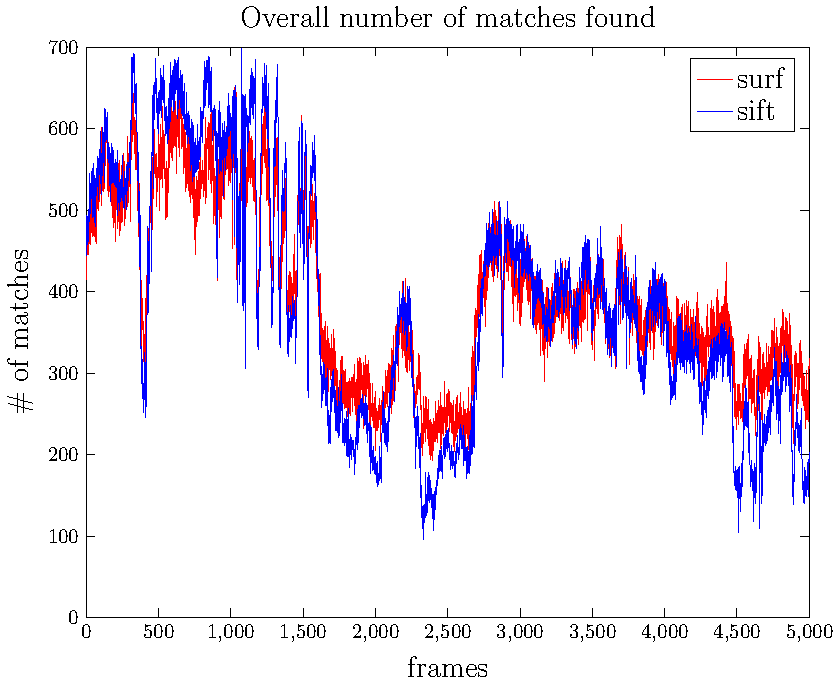
\includegraphics[width=0.32\textwidth]{./figs/numMatches.pdf}
%   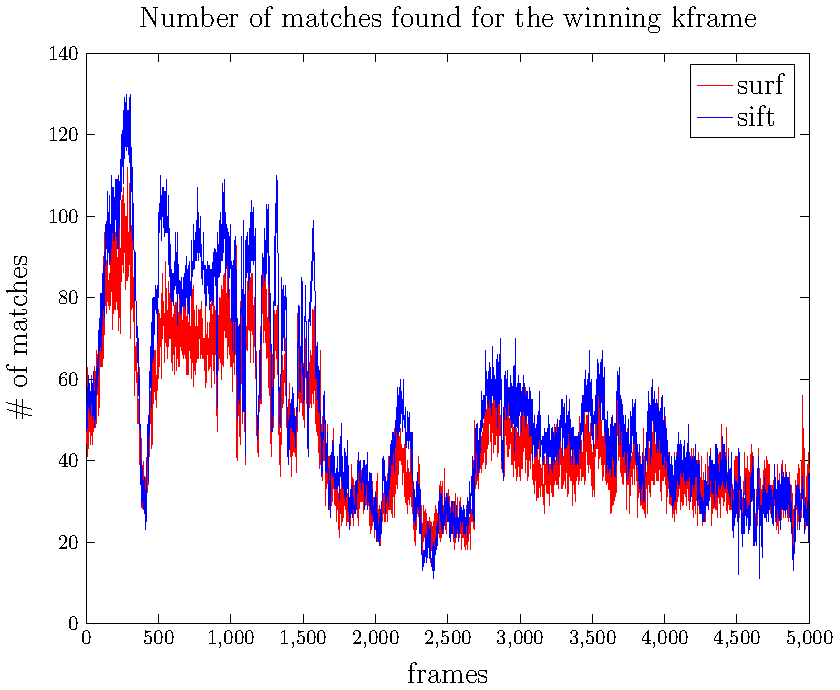
\includegraphics[width=0.32\textwidth]{./figs/numMatchesWinning.pdf}
%   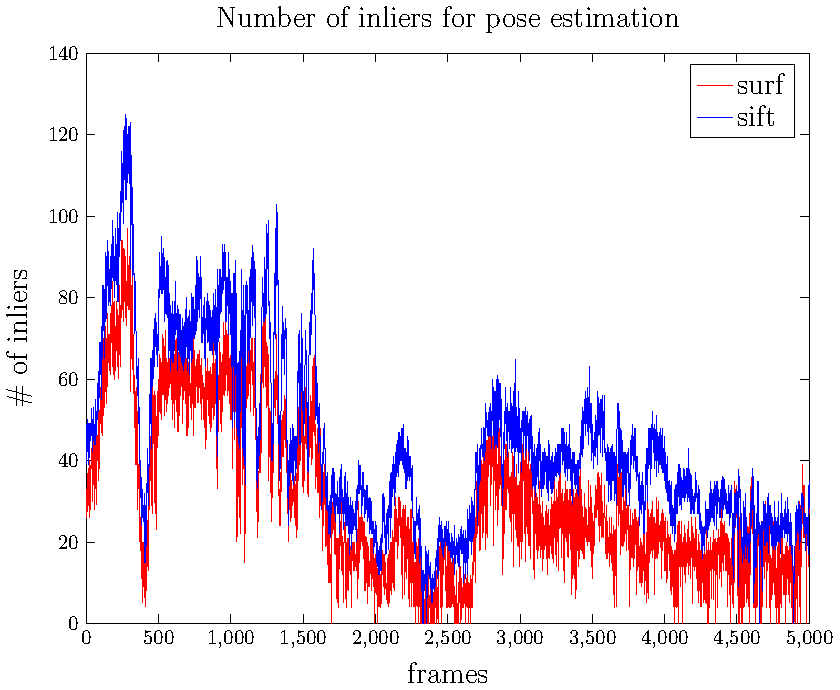
\includegraphics[width=0.32\textwidth]{./figs/numInliers.pdf}
% \caption{Comparison of the number of matches found using SURF (red) and SIFT (blue) over a sequence of $5000$ frames. The leftmost image shows the number of matches between $\mathcal{F}$ and $\mathcal{G}$ after the LRT, the center image shows the number of matches of the winning kframe and the rightmost image shows the number of inliers that supports the estimated pose.}
% \label{fig:numMatches}
% \end{figure*}

% \begin{figure*}
%   \centering
%   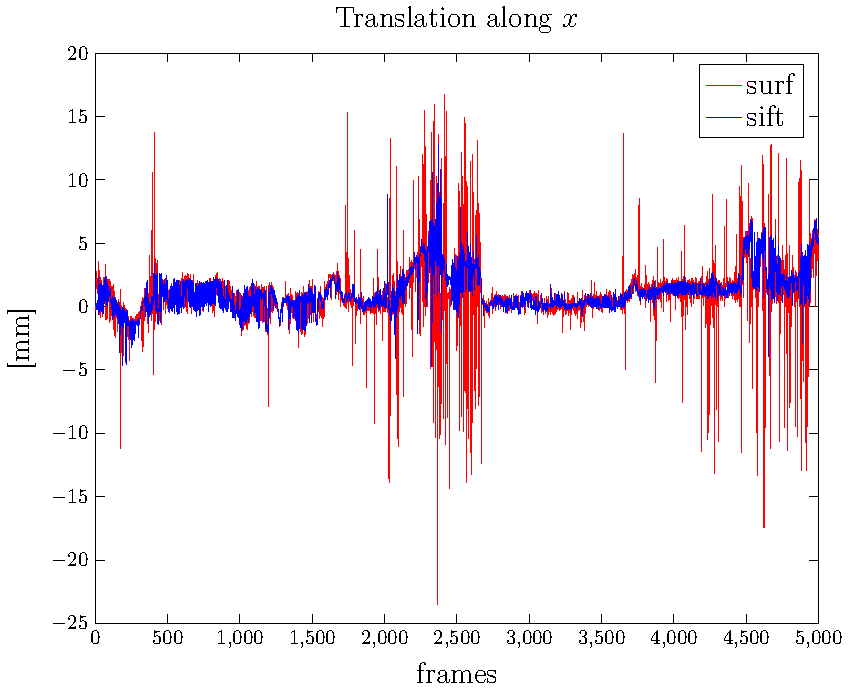
\includegraphics[width=0.32\textwidth]{./figs/translationX.pdf}
%   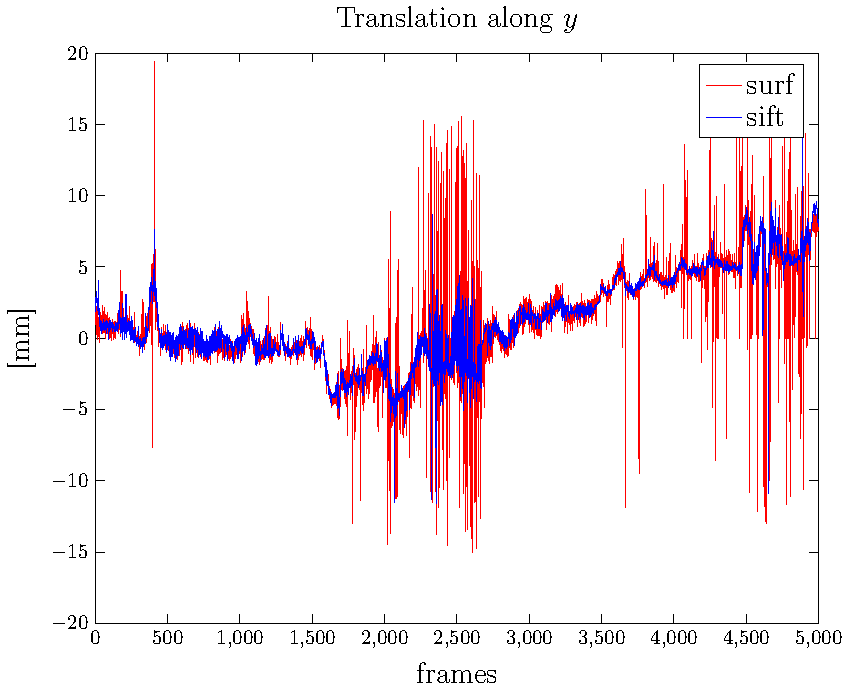
\includegraphics[width=0.32\textwidth]{./figs/translationY.pdf}
%   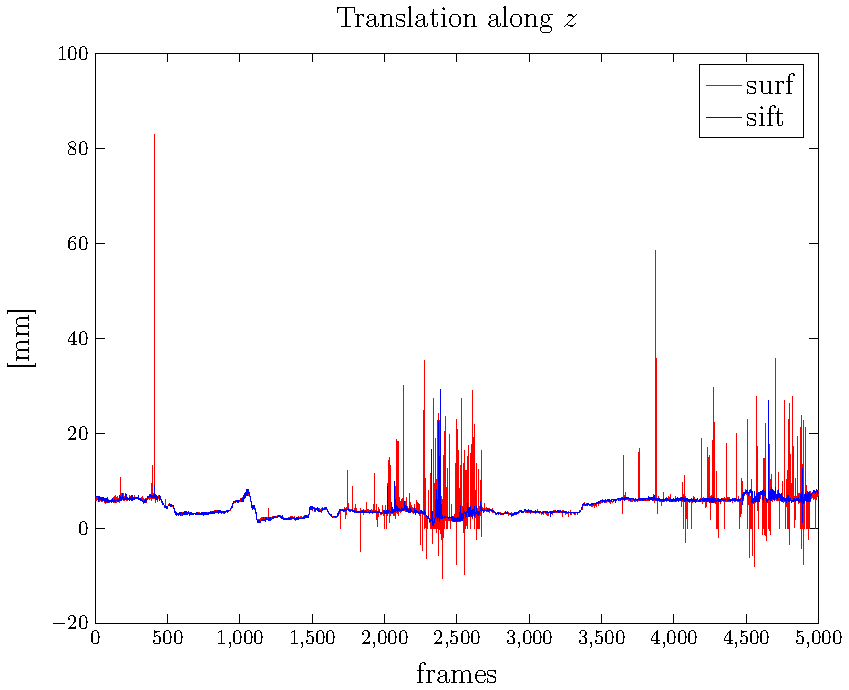
\includegraphics[width=0.32\textwidth]{./figs/translationZ.pdf}
%   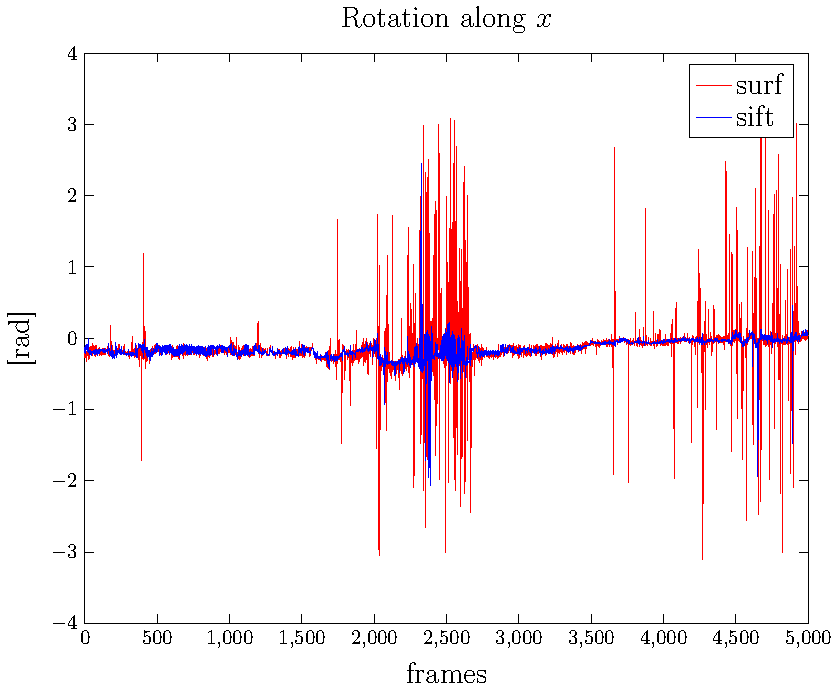
\includegraphics[width=0.32\textwidth]{./figs/rotationX.pdf}
%   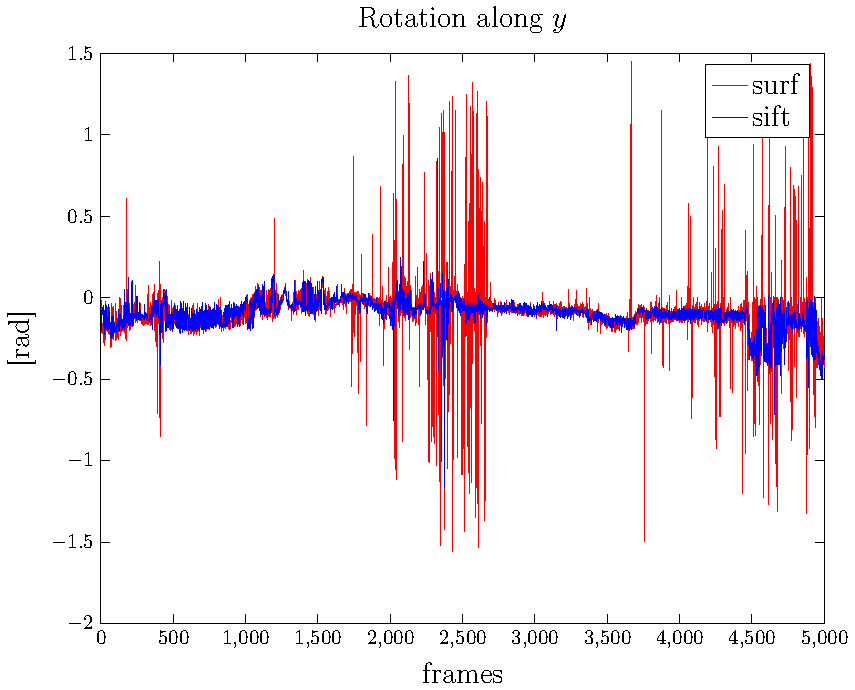
\includegraphics[width=0.32\textwidth]{./figs/rotationY.pdf}
%   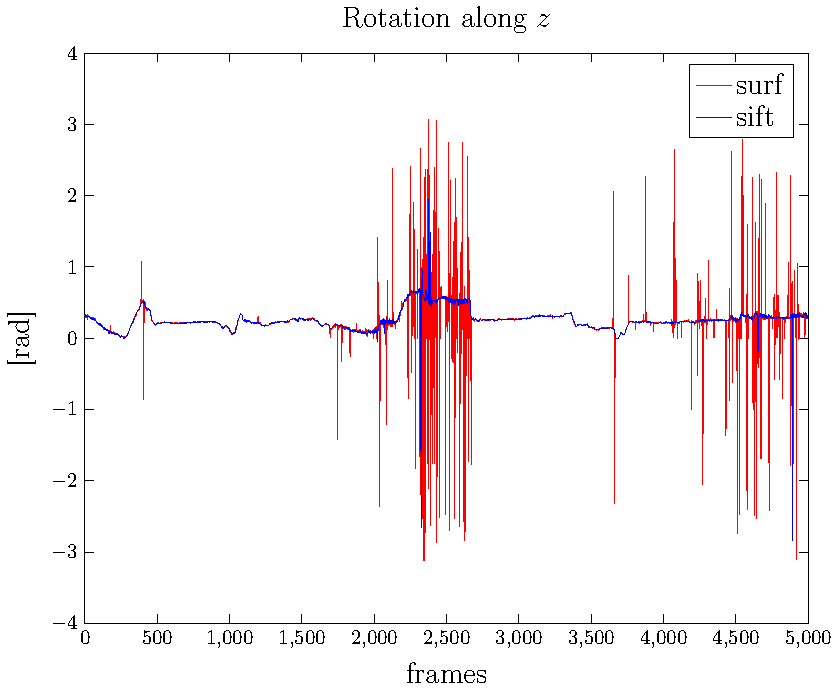
\includegraphics[width=0.32\textwidth]{./figs/rotationZ.pdf}
% \caption{Estimated pose components (top, translation $t_x$, $t_y$ and $t_z$, bottom rotation angles $r_x$, $r_y$ and $r_z$) using SURF (red) and SIFT (PopSift implementation) features over a sequence of $5000$ frames. It can be noted that SIFT enable a more stable and less jittered estimation of the components.}
% \label{fig:SurfVsSift}
% \end{figure*}




 

% \begin{figure}
%   \centering
%   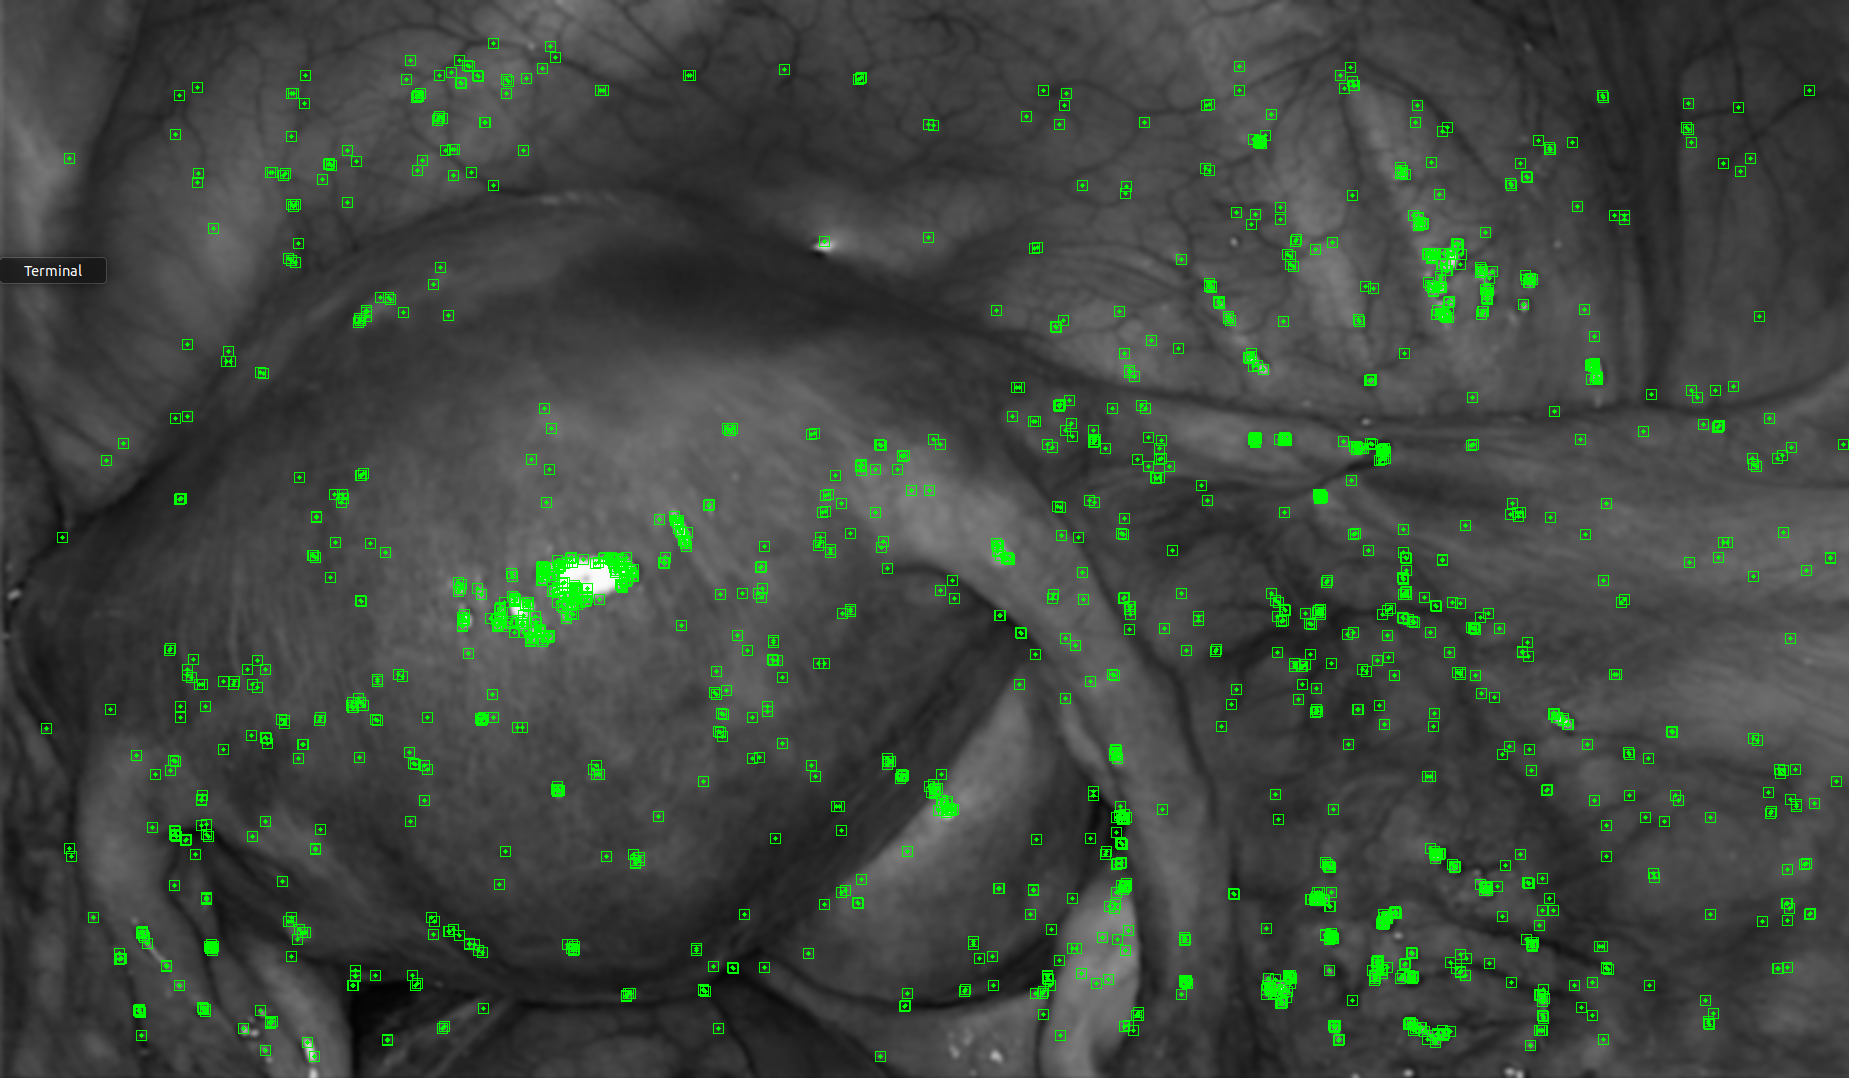
\includegraphics[width=0.45\columnwidth]{./figs/frame0001Features.png}
%   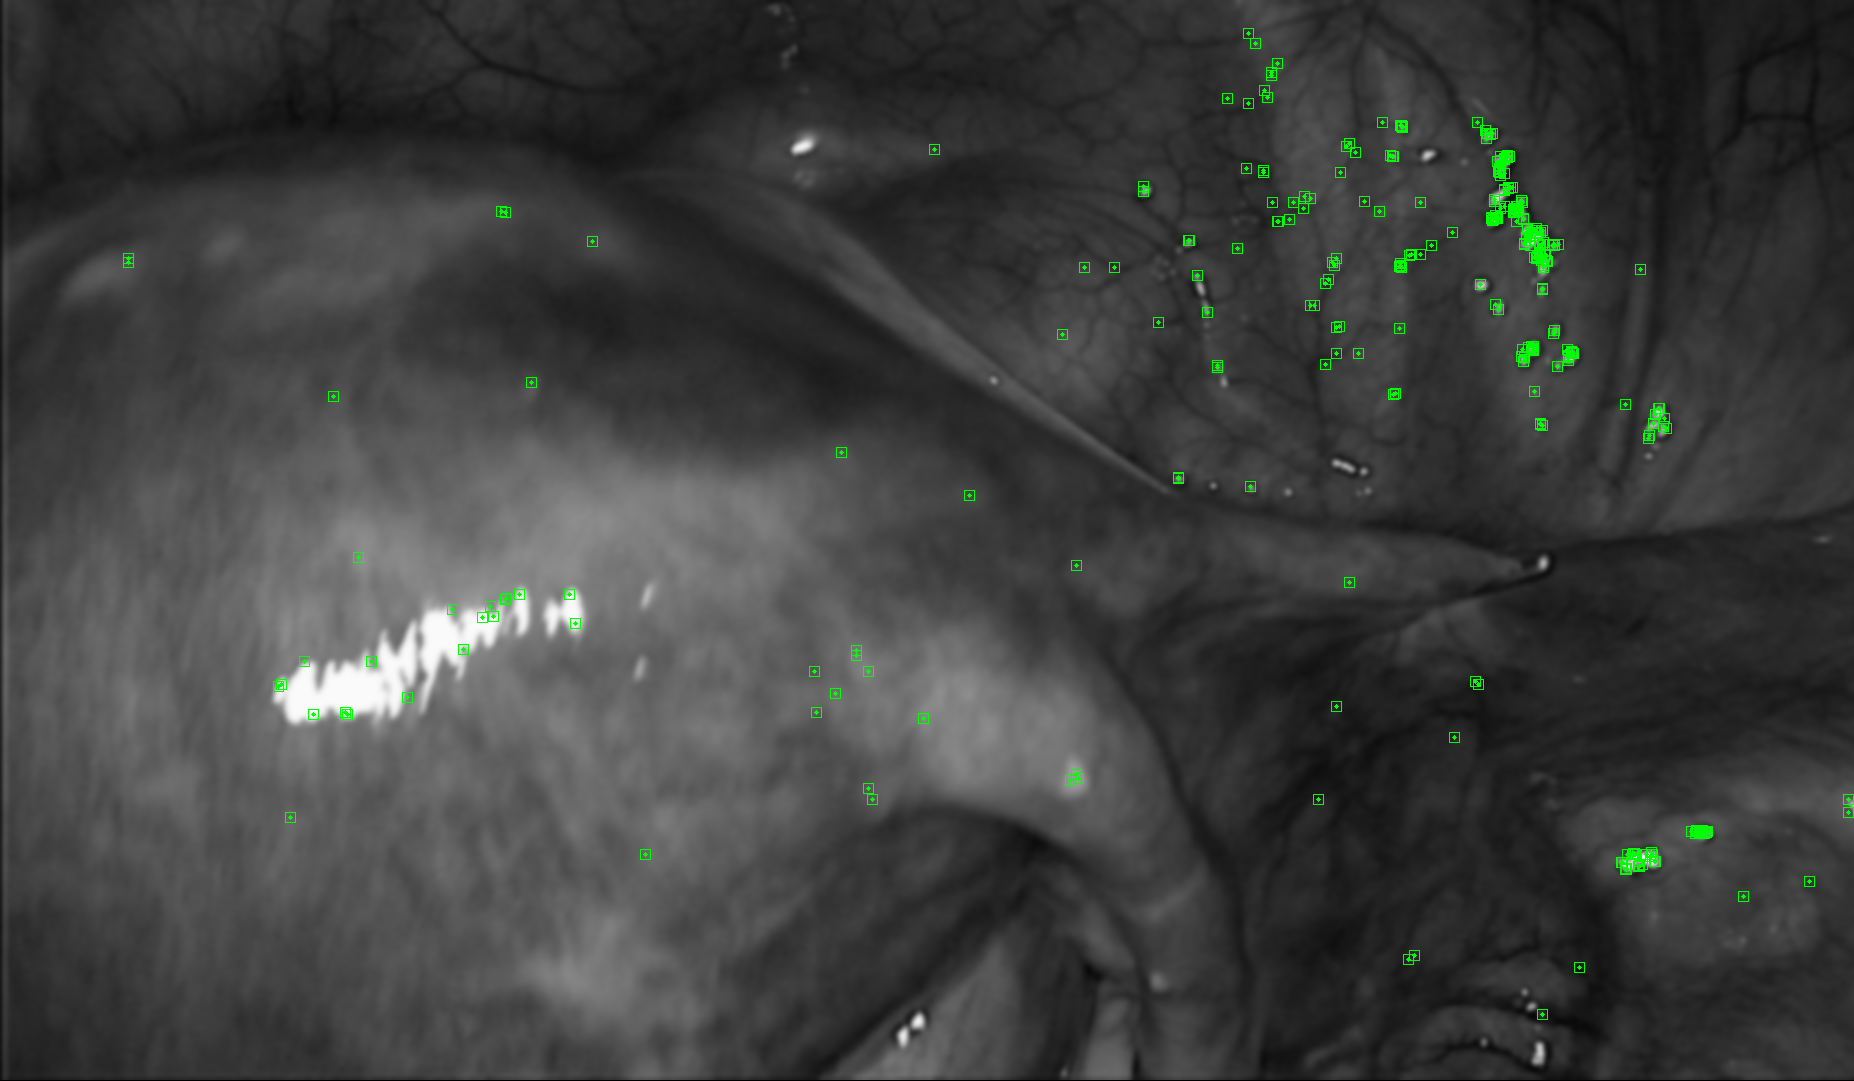
\includegraphics[width=0.45\columnwidth]{./figs/frame0107Features.png}
%   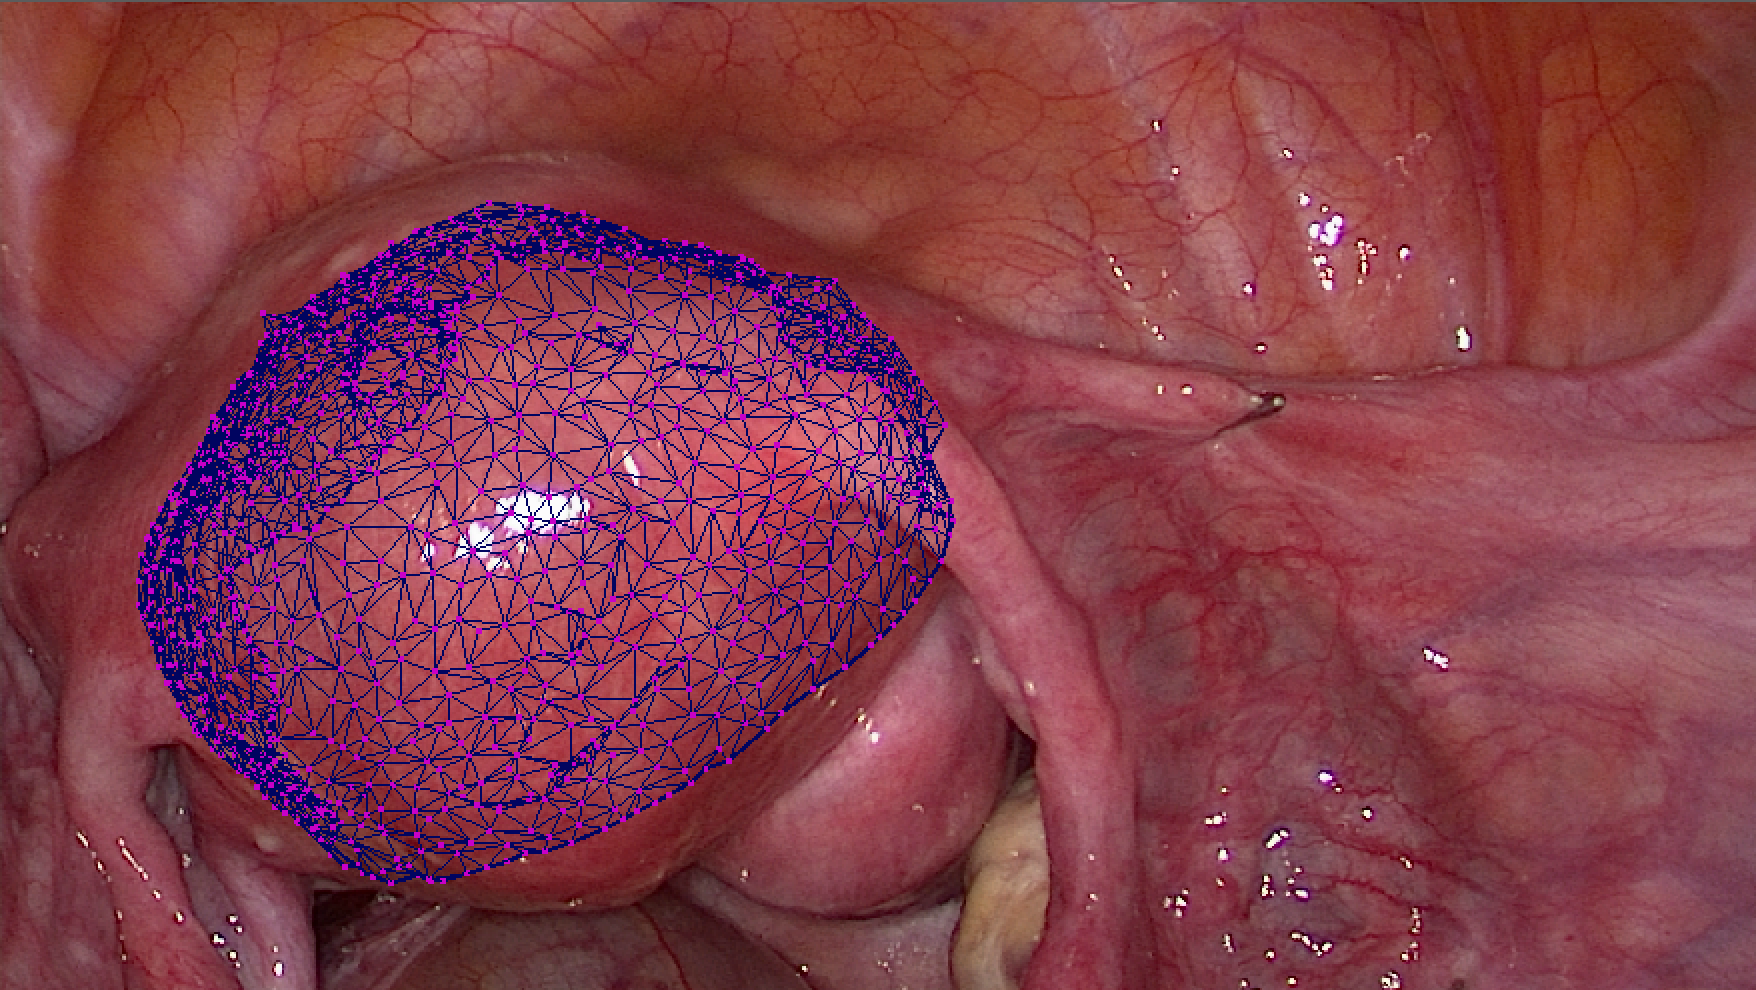
\includegraphics[width=0.45\columnwidth]{./figs/frame001.png}
%   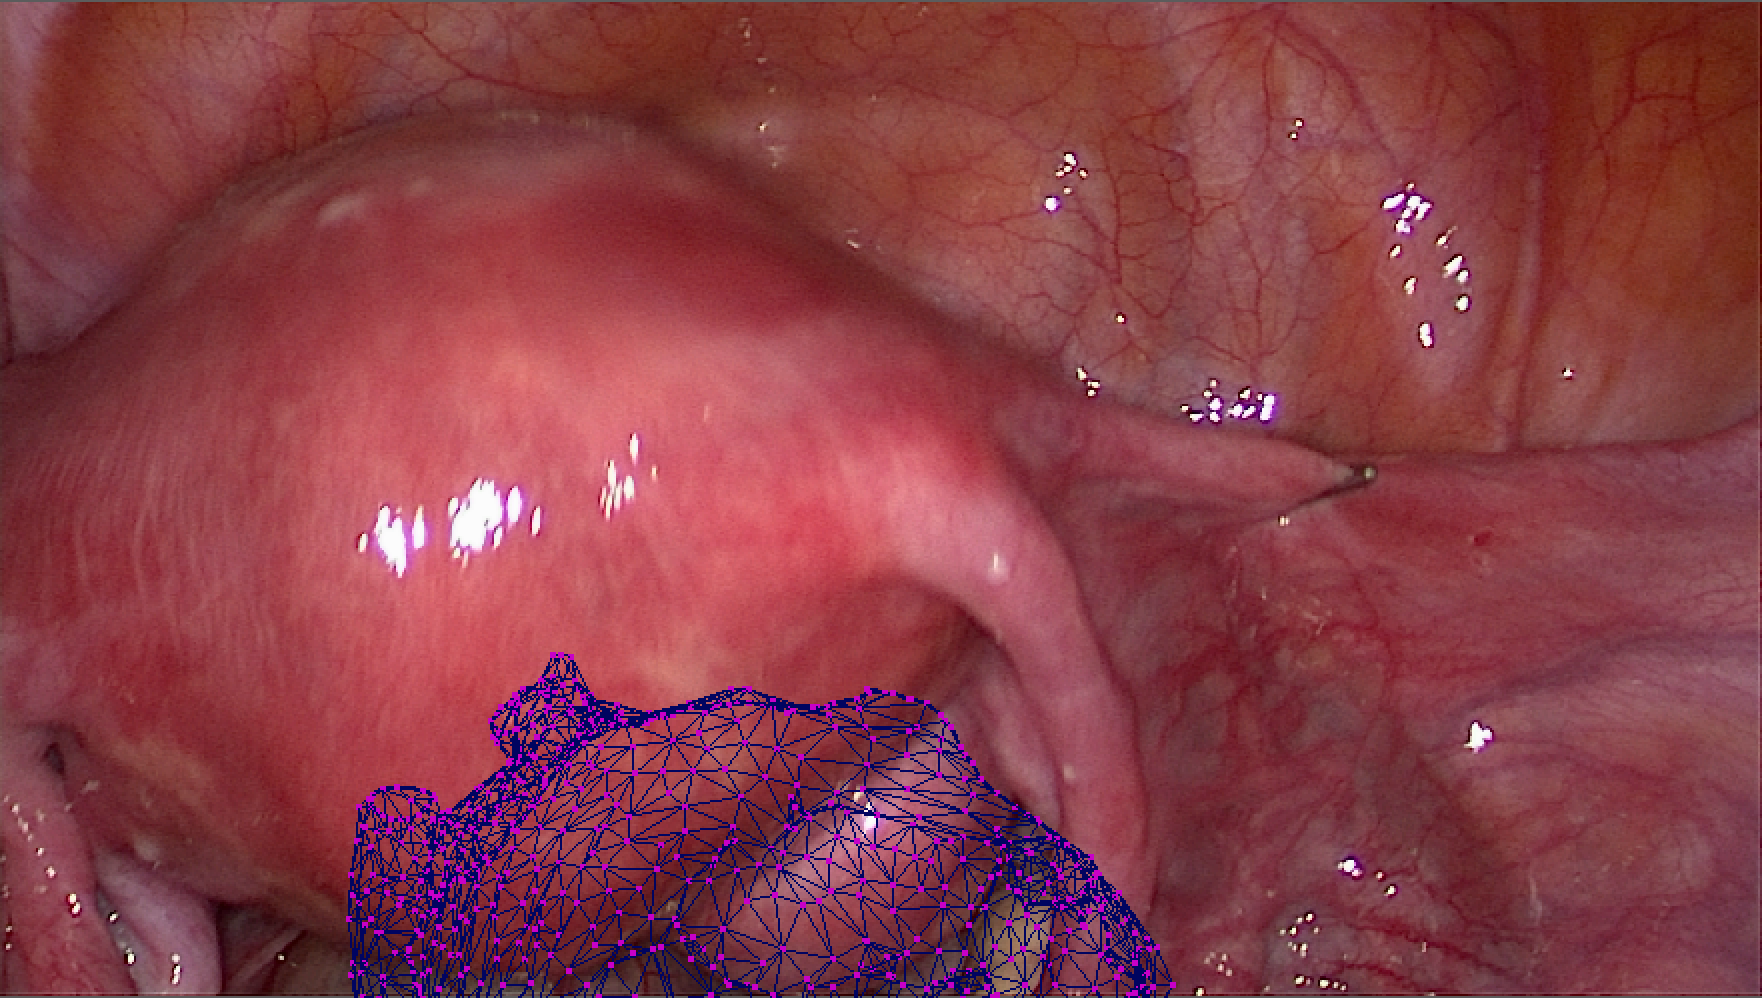
\includegraphics[width=0.45\columnwidth]{./figs/frame107.png}  
% \caption{An example of tracking issue of SLAM approaches: even if the model is correctly registered and tracked (left), it can happen that due to the movements of the organ and the occlusions the tracker tracks the camera pose \wrt the background thus affecting the AR visualization (right). }
% \label{fig:orbAR}
% \end{figure}


% % The input models used in the presented experiments are generated from T2 weighted MRI with segmentation done semi-automatically using MITK~\cite{Wolf_themedical}.
% % The deformation models that we experiment with are tetrahedral Finite Element Models (FEMs) built with a 3D vertex grid (\SI{6}{\milli\metre} spacing) cropped to the organ.
% % Therefore, $\vet{x}_t$ holds the unknown 3D positions of the FEM's vertices in laparoscope coordinates.
% % Trilinear interpolation was used to compute $f(\vet{p};\vet{x}_t)$.
% % For $\Einternal$ the Saint Venant-Kirchoff strain energy is used, with patient-generic values for the Young's modulus $E$ and Poisson's ratio $\nu$.
% These were for healthy kidney tissue $E=\SI{7}{\kilo\pascal}$, $\nu=0.43$~\cite{Li_TIP08}, 
% % For healthy uterus tissue we use $E=\SI{96}{\kilo\pascal}$, $\nu=0.45$~\cite{uterusModel} and $E=\SI{532}{\kilo\pascal}$, $\nu=0.48$ for myomas~\cite{uterusModel}.
%Note that in the registration problem there is always a balancing weight between the internal energy and energy coming from image cues (which have no real physical meaning).
%Therefore only the relative values of $E$ are important to us (with respect to the balancing weight), rather than their absolute values.

\subsubsection{Augmentation Results}
\fig{fig:myomas}(a) shows the preoperative data of a patient whose uterus contains a myoma (in green) of a size of $\SI{11.3}{\milli\metre}\times\SI{22.9}{\milli\metre}\times\SI{17.5}{\milli\metre}$.
The preoperative mesh of the uterus has $2488$ vertices and $4972$ faces.
From the exploratory video $15$ keyframes were extracted to perform MVS reconstruction, obtaining a 3D model of $1760$ vertices.
\fig{fig:myomas}(b) shows the successful alignment between the preoperative data and the MVS reconstruction.
The cost function \eq{eq:totalCost} was optimized in $6$ iterations in approximately \SI{21}{\second}.
In \fig{fig:myomas}(c) we show four keyframes used for the reconstruction together with an overlay of the uterus surface registered to each frame.
Qualitatively we see that the 3D preoperative model aligns well to the image of the uterus.
Finally, \fig{fig:myomas}(d) reports the visual augmentation of the myoma in some frames of a video recorded during surgery, clearly showing that the uterus is tracked well. 
The full video is provided as supplemental material along with videos from other patients.


% \begin{figure*}[t]
%   \centering
%   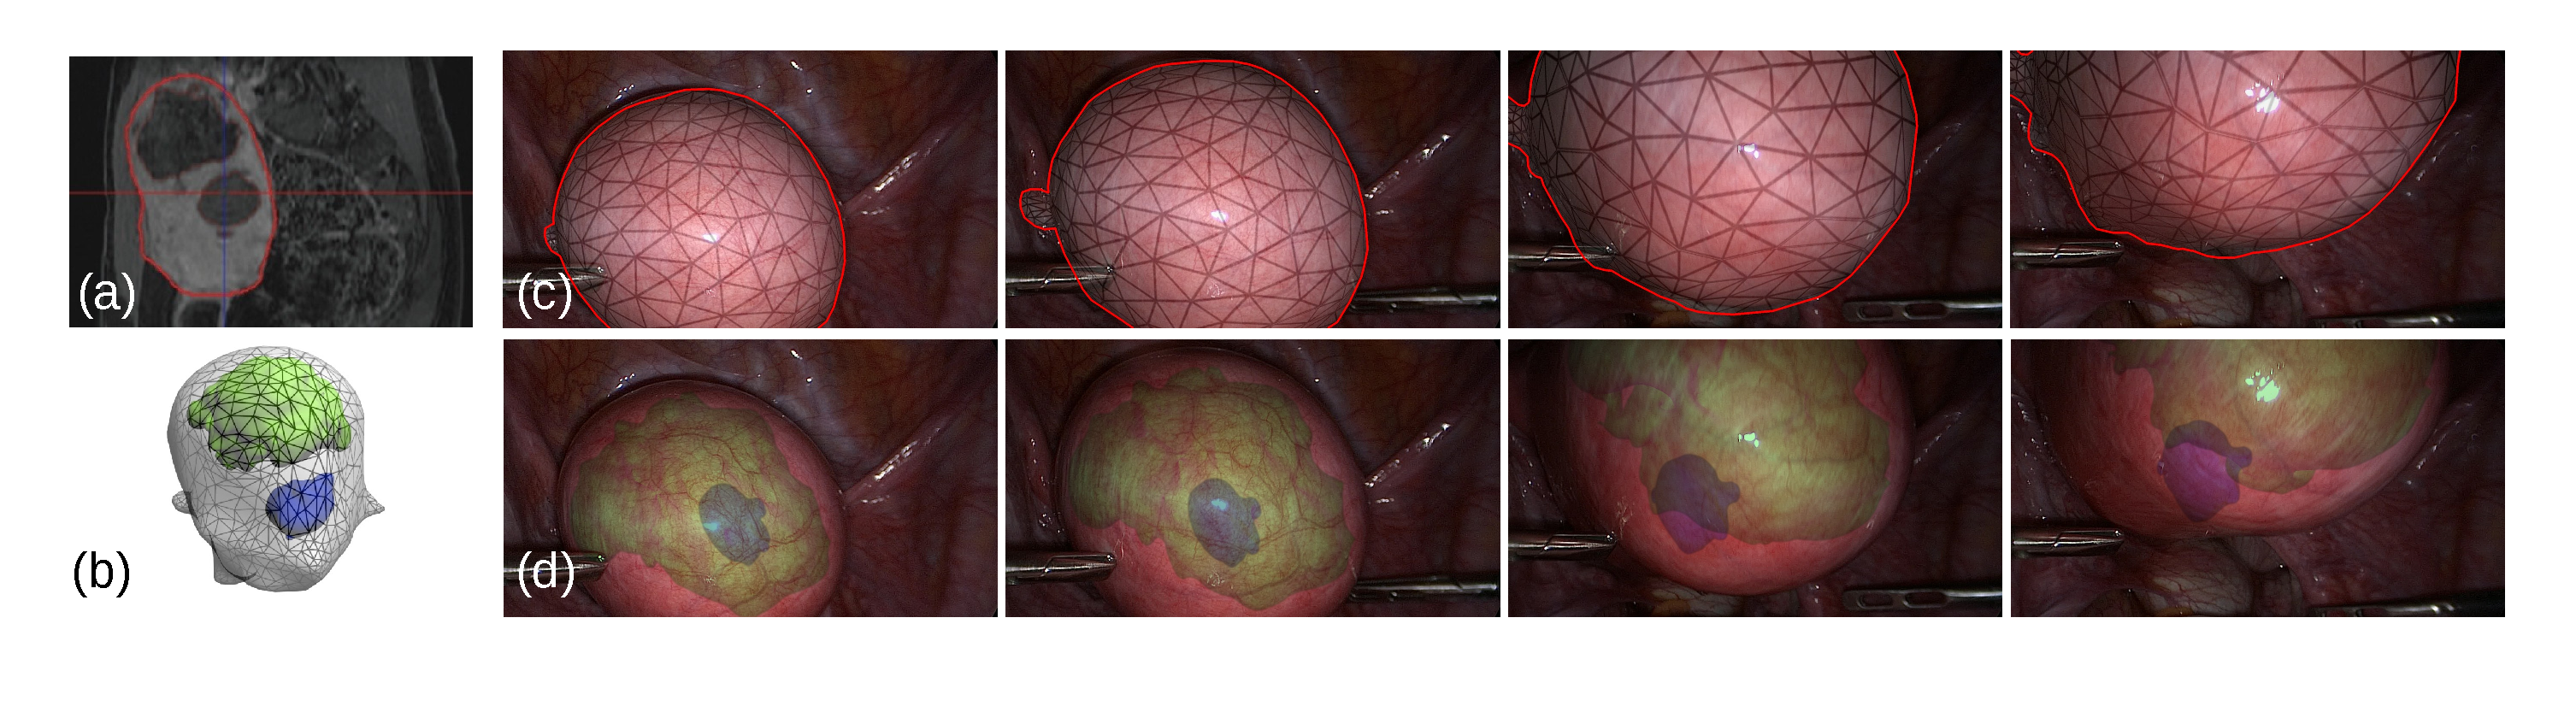
\includegraphics[width=\textwidth]{./figs/frames_aug.pdf}
% \caption{(a) The MRI preoperative data, (b) the 3D preoperative model of the uterus with the two myomas as reconstructed from the MRI, (c) frame from the video feed with the mesh model of the uterus from the MRI overlaid in each image and (d) its AR augmentation with the myomas shown as image overlay.}
% \label{fig:myomas}
% \end{figure*}
% Figures \fig{fig:myomas}(a) and \fig{fig:myomas}(b) show the preoperative data of a patient with two myomas. One myoma was large, with a diameter of \SI{121}{\milli\metre}, and the other medium sized with a diameter of \SI{52}{\milli\metre}. The preoperative mesh of the uterus has $6210$ vertices.
% %$\mathcal{M}$ was constructed by performing an interactive segmentation of the MRI using MITK~\cite{Wolf_themedical}, followed by meshing with marching cubes, two iterations of Laplacian mesh smoothing and then mesh decimation with quadratic edge collapse~\cite{conf/siggraph/GarlandH97} to give a mesh of $6210$ vertices. 
% The laparoscopic video was recorded during the patient's myomectomy and we performed the registration and augmentation off-line after surgery on a \SI{50}{\second} video clip before resection began (including the 20 second exploratory phase). We used $10$ keyframes to perform the SfM from the exploratory phase, and this computed correspondences for $321$ image features located on the uterus. The cost function in \eq{eq:totalCost} was optimised in $6$ iterations in approximately \SI{15}{\second}. % with our \CC implementation.
% % This took approximately \SI{15}{\second} to compute using an unoptimised Matlab implementation with a \CC $z$-buffer implementation.
% %The registration for the frames after the exploratory video was achieved using the method described in \sect{sec:registration}, which processed each frame in approximately \SI{37.0}{\milli\second} (or \SI{27}{fps}).
%  We show four frames from the clip in \fig{fig:myomas}(c), together with an overlay of the uterus surface registered to each frame. Its silhouette boundary is displayed in red. 
% %We show with a red contour the silhouette boundary of $\mathcal{M}$ in each frame.
% Qualitatively we see that the red contours align well to the real image contours shows clearly that the registration track the uterus well over the sequence. In \fig{fig:myomas}(d) we show the visual augmentation of the myomas in each frame (the larger myoma is in green and the smaller is in blue). The surgeon who conducted the myomectomy reported that localising the small myoma was difficult, and took them approximately $15$ minutes. After surgery they inspected our augmentations and confirmed that both myomas appeared to be localised well by the system. %This promising result indicates the potential benefit for using our AR system during surgery.
% %\begin{figure*}[ht]
% %  \centering
% %  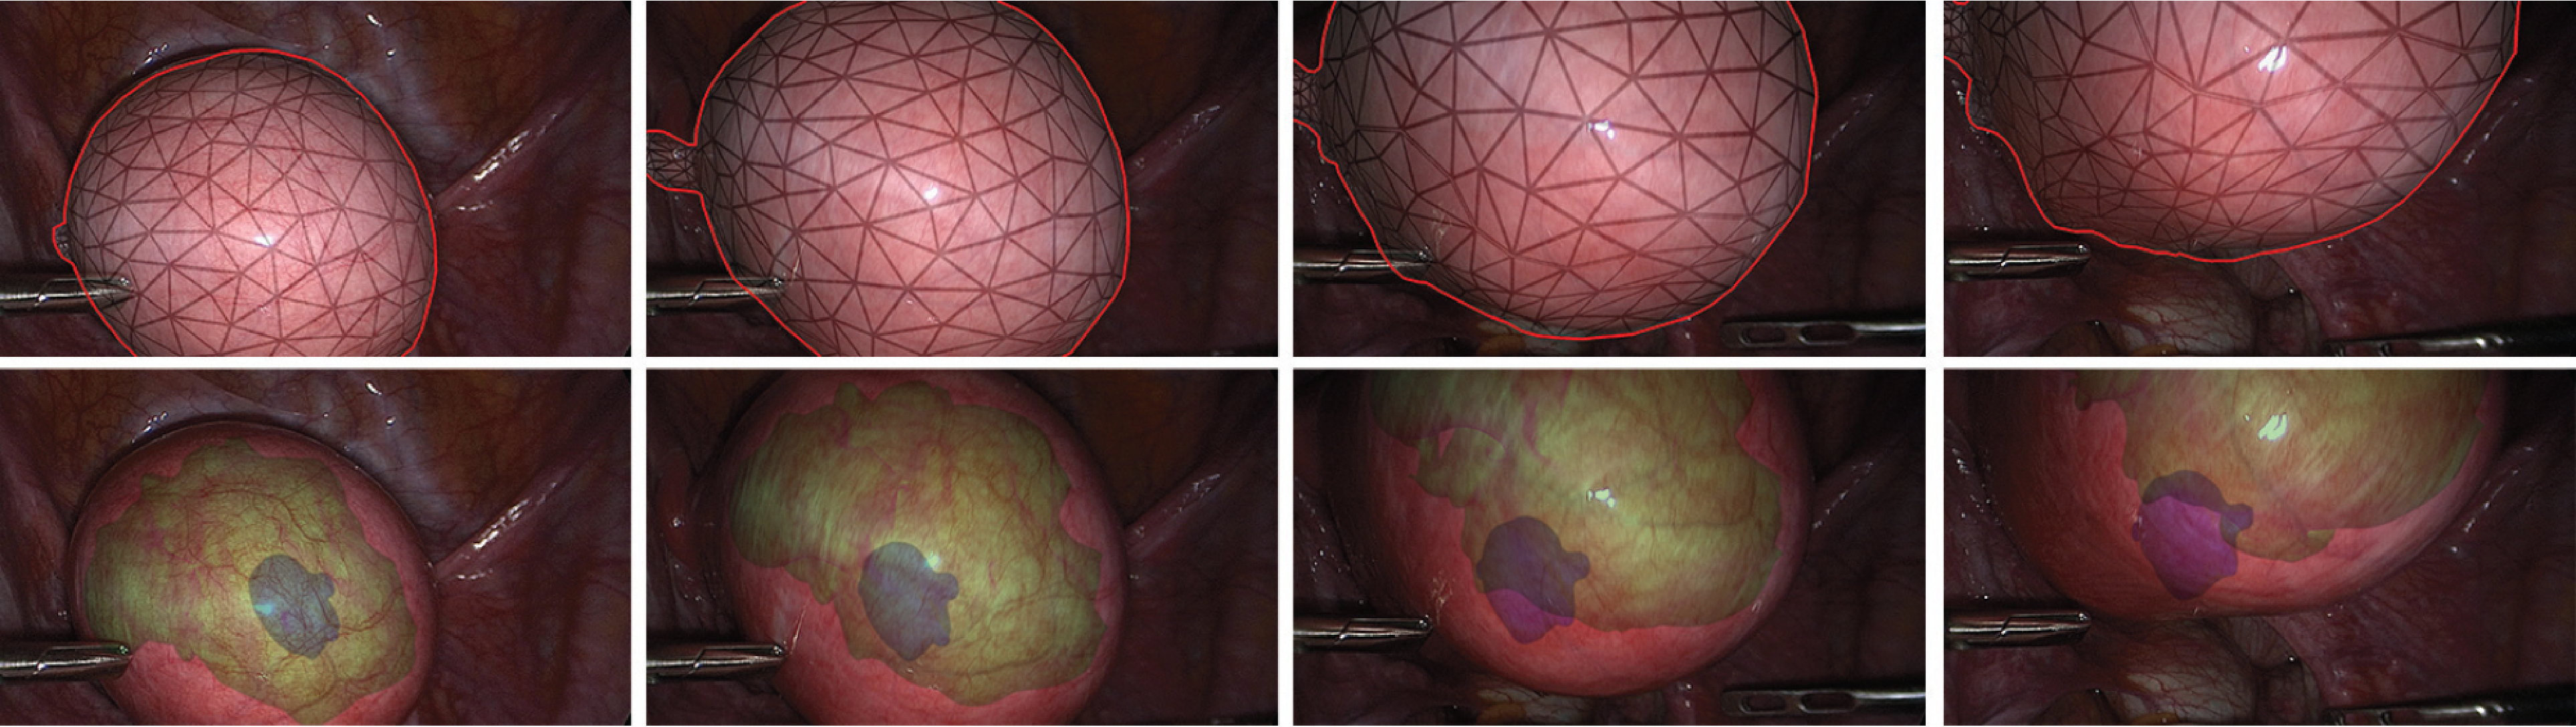
\includegraphics[width=0.75\textwidth]{./figs/invivoHumanUteri/qualitative.pdf}
% %  \caption{Registration between the uterus in a pre-operative MRI to intra-operative laparoscopic images, and visual augmentation of two hidden myomas.
% %The top row shows $\mathcal{M}$ (the mesh model of the uterus from the MRI ) overlaid in each image.
% %The red contours denote the silhouette boundaries of $\mathcal{M}$ in each image. The bottom row shows the augmented myomas.}
% %	\label{fig:qualResults}
% %\end{figure*}
% More experiments results are provided in the supplemental material (\url{https://bit.ly/2m9rGHH}).

% \subsection{Live usage and quantitative ex-vivo user evaluation with porcine kidneys}
% %\subsection{Overview}
% %\paragraph{Materials.}
%  We used $29$ porcine kidneys recovered from pigs operated after resident training. For each kidney pseudo-tumors were created by injecting alginate, a hardening hydrocolloid, of between \SI{4}{\milli\metre} and \SI{10}{\milli\metre} in diameter.
% In total $59$ pseudo-tumors were injected at arbitrary sub-surface positions, with an average of $2.5$ per kidney.
% We used safe tissue margins of \SI{5}{\milli\metre}.
% Kidney models were made as described in \sect{sec:inputModels} from 3T MRI images (\SI{0.4}{\milli\metre} resolution and slice thickness \SI{1.5}{\milli\metre}).
% The interventional equipment is shown in \fig{fig:visualCompare}\,(c) and consisted of a Karl Storz \SI{10}{\milli\metre} laparoscope column with CLARA image enhancement, a surgical grasper, an incision tool, a laparoscopic pelvic trainer and an instrument with a surgical marker pen attached at the tip (referred to as the \emph{marker instrument}).
% The AR software ran on a mid-range Intel i7 desktop workstation with an NVidia 980 Ti GPU, with visualisations shown on a \SI{26}{\inch} monitor.
% Laparosurgery was performed by a skilled final-year resident.
% The resident spent time training before evaluation to familiarise the task, the guidance software and to provide feedback to improve visualisation.
% In total $28$ pseudo-tumors were resected during this time. 


% \paragraph{AR guidance with Tool Access Visualisation.}
% \label{sec:toolPortProj}

%  Having registered, the final task is AR visualisation.
% We briefly describe \emph{Transparent Blending} (TB) visualisation, which is the previous approach used with monocular laparoscopes.
% It works by first rendering the tumors on the laparoscope's image plane, then a composite image is made by blending the render with the real image to give the impression the organ is transparent.
% An example from~\cite{Collins2044} is shown in \fig{fig:visualCompare}\,(a) where two myomas are visualised with TB.
% TB however has a serious limitation which has not been previously addressed, and we find it can actually \emph{mis-guide the surgeon}.
% The problem is illustrated in \fig{fig:mis-guidance}\,(a) and is as follows.
% When a surgeon actually uses TB to resect a tumor they usually assume it indicates where they should cut to access the tumor.
% This however is incorrect.
% It just shows the position of the tumor from the viewpoint of the laparoscope.
% Often they assume the tumor's centre would be reached by cutting into the organ from the rendered tumor's centre $\mathbf{c}\in\mathbb{R}^2$.
% This is not the case as shown in \fig{fig:mis-guidance}\,(a).
% In our user study we found this is a significant problem with smaller and/or deeper tumors, and can cause them to be missed.
% % increases as the tumor's depth increases and the separation between the tool and laparoscope trocars increases. 
%   \begin{figure*}[h]
%   	\centering
%   	\includegraphics[width=0.9\textwidth]{./figs/kidneyUserStudy/visualisationCompare.pdf}
%   	\caption{(a) AR with Transparent Blending (TB) visualisation taken from~\cite{Collins2044}. (b) Our AR visualisation combining Transparent Blending with Tool Access Visualisation. (c) Our AR system in live operation during the ex-vivo user study.% (c) tumor margins marked on the organ's surface using Tool-port Projection visualisation with a surgical marker. The marks are then used to guide the surgon during tumor resection.
%   	}
%   	\label{fig:visualCompare}
%   \end{figure*}

%  \begin{figure*}%\textbf{}
%  	\centering
%  	\subfloat[AR with Render Blending]{{\includegraphics[width=5.4cm]{./figs/kidneyUserStudy/marginVisual1.pdf} }}%
%  	\qquad
%  	\subfloat[AR with Tool Access Visualisation]{{\includegraphics[width=5.4cm]{./figs/kidneyUserStudy/marginVisual2.pdf} }}%
%  	\caption{The difference between typical AR visualisation of a tumor (a), which does not take into account the position and access direction of the incision tool, and the proposed Tool Access Visualisation (b) which does.}%
%  	\label{fig:mis-guidance}%
%  \end{figure*}
 
% What the surgeon actually wants is to be shown how to reach the tumor using the incision tool.
% Furthermore, surgeons typically want to also see the tumor's safe tissue margin.
% We provide both information with what we call \emph{Tool Access Visualisation}, which is shown in \fig{fig:visualCompare}\,(b).
% Its associated geometry is shown in \fig{fig:mis-guidance}\,(b).
% {Tool Access Visualisation works by showing the tumor's safe tissue margin projected onto the organ's surface as a ring, which we call the \emph{tumor guidance ring}.
% The idea is that if the surgeon were to cut into the organ along the guidance ring, they would segment the tumor with a minimal margin of $w\,$mm.
% At present we do not visualise uncertainty in the margin's location, which is important for real clinical use, and leave this to future work.\textbf{}
  	
% We achieve Tool Access Visualisation with \emph{two} projections.
% The first is a perspective projection of the margin's surface onto the organ's surface, using a centre-of-projection located at the incision tool's port centre $\mathbf{p}\in\mathbb{R}^3$.
% The second is a perspective projection of the projected margin's perimeter onto the laparoscope's optical image (shown as rings in \fig{fig:visualCompare}\,(b)).
% To achieve this we need to know $\mathbf{p}$.
% Recall that the organ has been registered in laparoscope coordinates, therefore we need $\mathbf{p}$ in laparoscope coordinates.
% It may be possible to estimate $\mathbf{p}$ automatically using external and/or internal tool tracking, however this is left to future work.
% Here we assume $\mathbf{p}$ is given \textit{a priori}.
% In our user study, where the ports are located on a pelvic trainer, this is simple and can be done offline by taking physical measurements.
% We complete the visualisation by combining Tool Access Visualisation with TB visualisation (\fig{fig:visualCompare}\,(b))  to show tumors (solid fill), organ (wireframe) and safe tissue margins (wireframe).



% \paragraph{Interventional Protocol and Equipment}
% Laparosurgery was performed using the pelvic trainer, with the kidney inserted on a ground surface and the laparoscope and instruments inserted through three ports.
% The same port configuration was used in all cases.
% The surgeon was tasked to remove each tumor by cutting out a conic tissue section which included the tumor and its safe tissue margin.
% The kidneys were divided into two groups (non-randomised): the \emph{AR group} and the \emph{Non-AR group}, with 13 kidneys in the AR group with 29 tumors, and 19 kidneys in the Non-AR group with 33 tumors.
% Kidneys in the AR group were operated with the AR guidance system activated.
% Recall that the guidance system is not designed to handle significant deformation or topology change after the initial registration, which occurs when a tumor is resected.
% This was dealt with in the protocol by having the surgeon first mark dots along the tumor guidance ring using the marker instrument, guided by the AR visualisation.
% Once completed they used the marks to guide the resection with AR disactivated.
% For the Non-AR group, the surgeon first consulted the MRI using interactive slice-based visualisation~\cite{Wolf_themedical}.
% The task was then performed without AR guidance using the same safe tissue margin of \SI{5}{\milli\metre}.
 
 
% \paragraph{Results}
% We present results with the negative margin rate.
% A negative margin occurs when the tumor is contained entirely within the resected tissue.
% A positive margin occurs when either the tumor is completely absent from the resected tissue (a \emph{complete miss}), or if it is partially contained (a \emph{contact}).
% For three tumors the protocol was not completed properly (the conic section did not cut fully through the kidney) and were excluded.
% There were $13$ negative margins in the Non-AR group (\SI{41.9}{\percent}), with $4$ complete misses and $14$ contacts.
% There were $23$ negative margins in the AR group (\SI{85.2}{\percent}), with $0$ complete misses and $4$ contacts.
% Statistical significance was measured with Fisher's exact two-tailed test with  $p=0.0010$.
% Therefore the user study indicates a very significant benefit for using the AR guidance system.
\subsection{Use with Patients in the Operating Room}\label{subsec:use-with-patients-in-the-operating-room}
We tested our AR system in laparoscopic surgery~\cite{bourdel2017} and report on three patients with one, three and two uterine myomas respectively. 
We built the 3D preoperative models of the organ and the myomas from preoperative T2-weighted MR\@.
% Three-dimensional models of the patient uteri and myomas were constructed before surgery from T2-weighted MR. 
We used our system so that the surgeon could see the location of the myomas in real time. 

In \fig{fig:realOR}(a) we show the MR of the first patient with a $\SI{6}{\centi\metre}$ uterine myoma. \fig{fig:realOR}(b) shows the augmentation of the myoma and \fig{fig:realOR}(c) shows its resection.
At that stage our algorithm shows a past augmentation due to the changes in the uterus surface.
In \fig{fig:realOR}(d) we show our system deployed in the operating room.
The MR of the second patient is shown in \fig{fig:realOR}(e), showing three myomas that are visualized with AR in \fig{fig:realOR}(f,g,h).
The third patient had two myomas whose segmentation from MR is shown in \fig{fig:realOR}(i).
Examples of augmentation of the myomas using bright colors and the uterine cavity mesh are displayed in \fig{fig:realOR}(j,k,m).
We recall that this is the first time one demonstrates markerless registration and AR during \emph{live} laparoscopic surgery. \SG{In our experience both the initial and tracking AR stages are valuable to the surgeon. The first stage is necessary to give the first appreciation of hidden structure locations (tumours and the uterine canal). Recall however that the surgeon is using a monocular camera. The value of the tracking stage is to give the sensation of depth and parallax, and to help orient the uterus to establish a good resection plane. Specifically, the surgeon can move the uterus with the cannula and they receive interactive visual feedback. Depth and spatial comprehension of sub-surface structures are easier because of motion and parallax effects.} 
 



\section{Discussion}
\label{sec:discussion}
\SG{The proposed framework is the first complete markerless real-time
AR guidance system for laparoscopic surgery of the uterus.
Its major advantage is that it does not require special hardware and works with a standard monocular laparoscope and an off-the-shelf computer.
This enables a quick set-up in the OR, where no other hardware should interfere, perturb or distract the surgeon.
Overall, the required steps for calibration, 3D reconstruction and registration take around $\sim\SI{10}{\minute}$.
Most of the interactive and manual operations, such as the masking and the contour annotations are carried out by an operator and can be done in parallel while the surgeon proceeds with other surgery tasks (\eg clamping).
Thus the impact on the clinical activity of the surgeon is limited to acquiring images for the calibration and the 3D reconstruction.
Concerning AR and the visual feedback, the experiments show that the proposed approach for tracking is robust and responsive.
It runs in real-time with very low jitter, further mitigated by adding keyframes.
One of the limitations of our system is that it  relies on a few manual interactions.
This will drive our research directions to further improve usability and accuracy.
First is masking of the keyframes for 3D reconstruction.
Even if the effort is mitigated by the touchscreen (overall time kept under a minute), automatically detecting the organ in the image would further the usability.
We are investigating the use of CNNs to automatically extract the occluding contour fragments for initial registration~\cite{Francois2020}, but while the first results are encouraging, some more efforts are required to robustly integrate it in the pipeline.
As for the tracking part, an interesting and challenging research direction is to automate the addition of keyframes.
This is non-trivial because of the potential for drift caused by the accumulation of small registration errors. Finally, we now are planning a follow-up clinical trial using a hybrid OR with interventional CT imaging to quantify TRE with patients in the OR, which is a notoriously difficult task, \SGG{following the ideas proposed in~\cite{Bernhardt2016}}.
}

  
%\section{Conclusion}
%\label{sec:conclusion}
%We have presented the first complete markerless real-time AR guidance system for laparascopic surgery of the uterus. This works with a standard monocular laparoscope and does not require any additional tracking equipment. Numerous technical challenges are overcome with novel contributions as summarized in \S\ref{sec:contributions}. There are several directions for future work. Firstly we will extend the tracking approach to automatically add new keyframes to the keyframe set, to account for appearance change during surgery. This is non-trivial because of the potential for drift caused by the accumulation of small registration errors. Secondly, we aim to automate the extraction of occluding contour fragments using Convolutional Neural Networks, thus reducing need for manual effort during the initial registration. Unlike previous works we have demonstrated the viability of the approach in real clinical settings in the OR, and our objective now is to start a clinical trial to measure the clinical benefit in terms of reduction of procedure time and complication rate.

%The pipeline is composed of two main registration steps. The initial registration is performed at the early stage of surgery and it registers an MVS 3D reconstruction of laparoscopic images with the pre-operative model. To this end, we described a novel registration method that determines the change of state of the organ between its pre-operative state and the intra-operative reference state, while simultaneously resolving the reconstruction scale ambiguity. This has not been previously achieved for the uterus or indeed any other organ in previous literature. The second step is robust real-time tracking, which is performed live and registers each frame of the laparoscope video to the organ model with a
%novel tracking-by-detection approach. This outperforms previous state-of-the-art tracking, based on SLAM, by a wide margin. %The main technical novelties expand from the use of multiple reference images to assist both steps. For the initial registration, it allows us to obtain occluding contour and surface matching constraints from multiple viewpoints, which through quantitative evaluation is shown to significantly improve registration accuracy. Secondly, it allows us to obtain a diverse set of photometric features from different viewpoints, thus allowing better surface coverage of features, and to overcome the limited viewpoint invariance of state-of-the-art feature detectors such as SIFT and SURF. Unlike previous works for long-duration markerless tracking of monocular laparoscopic environments based on SLAM, we do not assume the scene is globally rigid, and this allows us to tackle the registration of a highly mobile organ such as the uterus. 




%oth to improve the initial registration process via occluding contour and surface fitting constraints from multiple views
%The current frame is matched with all the images used for the MVS reconstruction and the one getting more matches is retained to compute the resection.
%Contrary to SLAM-based approaches, each frame is registered independently from the others, thus being robust to occlusions and being able to easily recover whenever the tracking is lost because of, \eg, large occlusions.
%The effectiveness of the method has been tested on both synthetic and real data, showing that it can accurately register the pre-operative model and the model obtained by MVS reconstruction.
%We showed that the use of a real-time implementation of SIFT significantly improves the performances in terms of the number of registered frames and camera trajectory stability. 
%For these reason, since most of the steps require very little manual intervention, the proposed pipeline is very suitable for the use in a real case scenario. 



% Can use something like this to put references on a page
% by themselves when using endfloat and the captionsoff option.
\ifCLASSOPTIONcaptionsoff
  \newpage
\fi



% trigger a \newpage just before the given reference
% number - used to balance the columns on the last page
% adjust value as needed - may need to be readjusted if
% the document is modified later
%\IEEEtriggeratref{8}
% The "triggered" command can be changed if desired:
%\IEEEtriggercmd{\enlargethispage{-5in}}

% references section

% can use a bibliography generated by BibTeX as a .bbl file
% BibTeX documentation can be easily obtained at:
% http://mirror.ctan.org/biblio/bibtex/contrib/doc/
% The IEEEtran BibTeX style support page is at:
% http://www.michaelshell.org/tex/ieeetran/bibtex/
%\bibliographystyle{IEEEtran}
% argument is your BibTeX string definitions and bibliography database(s)
%\bibliography{IEEEabrv,../bib/paper}
%
% <OR> manually copy in the resultant .bbl file
% set second argument of \begin to the number of references
% (used to reserve space for the reference number labels box)
\bibliographystyle{IEEEtran}
% \bibliographystyle{plain}
\bibliography{IEEEabrv,bibliog}
% that's all folks


% % biography section
% % 
% % If you have an EPS/PDF photo (graphicx package needed) extra braces are
% % needed around the contents of the optional argument to biography to prevent
% % the LaTeX parser from getting confused when it sees the complicated
% % \includegraphics command within an optional argument. (You could create
% % your own custom macro containing the \includegraphics command to make things
% % simpler here.)
% %\begin{IEEEbiography}[{\includegraphics[width=1in,height=1.25in,clip,keepaspectratio]{mshell}}]{Michael Shell}
% % or if you just want to reserve a space for a photo:

% \begin{IEEEbiography}{Michael Shell}
% Biography text here.
% \end{IEEEbiography}

% % if you will not have a photo at all:
% \begin{IEEEbiographynophoto}{John Doe}
% Biography text here.
% \end{IEEEbiographynophoto}

% % insert where needed to balance the two columns on the last page with
% % biographies
% %\newpage

% \begin{IEEEbiographynophoto}{Jane Doe}
% Biography text here.
% \end{IEEEbiographynophoto}

% % You can push biographies down or up by placing
% % a \vfill before or after them. The appropriate
% % use of \vfill depends on what kind of text is
% % on the last page and whether or not the columns
% % are being equalized.

% %\vfill

% % Can be used to pull up biographies so that the bottom of the last one
% % is flush with the other column.
% %\enlargethispage{-5in}

\end{document}


